\documentclass[10pt,openany]{book}
% ------------------------------------------------------------
% Preamble for 「Pythonによる はじめての銀河シミュレーション」
% 157 x 221 mm layout based on the supplied textbook template.
% Compile with XeLaTeX.
% ------------------------------------------------------------
\usepackage[paperwidth=157mm,paperheight=221mm,margin=14mm,headheight=14pt,headsep=6mm]{geometry}
\usepackage{amsmath,amssymb,mathtools,bm}
\usepackage{graphicx,rotating,float,placeins,caption}
\captionsetup{font=small,labelfont=bf,labelsep=quad}
\graphicspath{{figures/}{./}}
\usepackage{fontspec}
\usepackage{xeCJK}
\IfFontExistsTF{Latin Modern Roman}{\setmainfont{Latin Modern Roman}}{\setmainfont{Liberation Serif}}
\IfFontExistsTF{Latin Modern Sans}{\setsansfont{Latin Modern Sans}}{\setsansfont{Liberation Sans}}
\IfFontExistsTF{DejaVu Sans Mono}{\setmonofont{DejaVu Sans Mono}[Scale=0.91]}{}
\setCJKmainfont{Noto Serif CJK JP}[ItalicFont={Noto Serif CJK JP}]
\setCJKsansfont{Noto Sans CJK JP}
\setCJKmonofont{Noto Sans Mono CJK JP}[Scale=0.90]
\xeCJKsetup{CJKmath=true}
\XeTeXlinebreaklocale "ja"
\XeTeXlinebreakskip = 0pt plus 0.1pt minus 0.01pt

\usepackage{xcolor,enumitem,array,booktabs,tabularx,xurl,etoolbox,needspace,fvextra}
\usepackage{fix-cm}

% TikZ settings are defined here rather than in a separate input file.
% This makes the project robust on Overleaf even when only the main preamble
% and chapter/figure files are copied into an existing project.
\usepackage{tikz}
\usetikzlibrary{arrows.meta,calc,positioning,patterns,decorations.pathreplacing,matrix}
\definecolor{figblue}{HTML}{0072B2}
\definecolor{figred}{HTML}{D55E00}
\definecolor{figgreen}{HTML}{009E73}
\definecolor{figgray}{HTML}{666666}
\tikzset{
  textbook diagram/.style={font=\sffamily\fontsize{9}{11}\selectfont,>=Latex,line width=0.6pt},
  vector/.style={-{Latex[length=2.1mm,width=1.4mm]},line width=0.85pt},
  guide/.style={draw=figgray,densely dashed,line width=0.5pt},
  state/.style={draw=black!50,fill=white,rounded corners=1pt,minimum width=48mm,minimum height=9mm,align=center},
  hint/.style={align=left,font=\sffamily\fontsize{8.5}{10.5}\selectfont},
  small label/.style={font=\sffamily\fontsize{8}{10}\selectfont}
}

\usepackage[most]{tcolorbox}
\usepackage{listings}
\usepackage{titlesec,fancyhdr}

\setlength{\parindent}{1em}
\setlength{\parskip}{0.15em}
\linespread{1.08}
\raggedbottom
\emergencystretch=1.5em
\widowpenalty=10000
\clubpenalty=10000

\definecolor{navy}{HTML}{0D1B3E}
\definecolor{amber}{HTML}{B5740F}
\definecolor{amberbg}{HTML}{FBF1E0}
\definecolor{cyan}{HTML}{1F6390}
\definecolor{cyanbg}{HTML}{E7F0F7}
\definecolor{navybg}{HTML}{EDF0F7}
\definecolor{rule}{HTML}{C9D2E3}
\definecolor{notegray}{HTML}{F3F5F6}
\definecolor{notegreen}{HTML}{287250}
\definecolor{warnred}{HTML}{9B4030}

% Article boxes: notebox/failbox. goalbox is a chapter-opening structural element.
\newtcolorbox{notebox}[1]{enhanced,breakable,colback=notegray,colframe=notegreen,
  boxrule=0.45pt,arc=1.5pt,left=2.8mm,right=2.8mm,top=2mm,bottom=2mm,
  fonttitle=\sffamily\bfseries,colbacktitle=notegreen!10,coltitle=notegreen,
  title={もう少し詳しく：#1},before skip=7pt,after skip=7pt}
\newtcolorbox{failbox}[1]{enhanced,breakable,colback=notegray,colframe=warnred,
  boxrule=0.45pt,arc=1.5pt,left=2.8mm,right=2.8mm,top=2mm,bottom=2mm,
  fonttitle=\sffamily\bfseries,colbacktitle=warnred!8,coltitle=warnred,
  title={よくある失敗：#1},before skip=7pt,after skip=7pt}
\newtcolorbox{goalbox}[1][本章の目標]{colback=cyanbg,colframe=cyan,coltitle=white,
  title={\sffamily #1},fonttitle=\bfseries,boxrule=0.7pt,arc=2pt,
  left=7pt,right=7pt,top=5pt,bottom=5pt,breakable}

\newcommand{\inputcode}[1]{\par\smallskip\noindent\begin{minipage}{\linewidth}\VerbatimInput[
  fontsize=\fontsize{7.5}{9.3}\selectfont,frame=lines,rulecolor=\color{navy!35},framesep=2.2mm,
  numbers=left,numbersep=4pt,breaklines=true,breakanywhere=true,tabsize=4]{generated/#1.py}\end{minipage}\par\smallskip}

\titleformat{\chapter}{\LARGE\bfseries\sffamily\color{navy}}{第\thechapter 章}{0.8em}{}
\titleformat{\section}{\large\bfseries\sffamily\color{navy}}{\thesection}{0.5em}{}
\titleformat{\subsection}{\normalsize\bfseries\sffamily\color{navy}}{\thesubsection}{0.5em}{}
\titlespacing*{\chapter}{0pt}{0pt}{12pt}
\titlespacing*{\section}{0pt}{1.1em}{0.4em}
\titlespacing*{\subsection}{0pt}{0.75em}{0.25em}
\pretocmd{\section}{\Needspace{6\baselineskip}}{}{}
\pretocmd{\subsection}{\Needspace{5\baselineskip}}{}{}
\setlist[itemize]{leftmargin=1.7em,itemsep=0.15em,topsep=0.25em}
\setlist[enumerate]{leftmargin=2em,itemsep=0.2em,topsep=0.3em}
\setcounter{tocdepth}{1}
\setcounter{secnumdepth}{2}

\pagestyle{fancy}
\fancyhf{}
\fancyhead[L]{\scriptsize\sffamily はじめての銀河シミュレーション}
\fancyhead[R]{\scriptsize\sffamily\nouppercase{\leftmark}}
\makeatletter
\renewcommand{\chaptermark}[1]{%
  \if@mainmatter
    \markboth{第\thechapter 章\enspace #1}{}%
  \else
    \markboth{#1}{}%
  \fi}
\makeatother
\fancyfoot[R]{\small\thepage}
\fancypagestyle{plain}{\fancyhf{}\fancyfoot[R]{\small\thepage}\renewcommand{\headrulewidth}{0pt}}

\newcommand{\rvec}{\boldsymbol r}
\newcommand{\vvec}{\boldsymbol v}
\newcommand{\avec}{\boldsymbol a}
\newcommand{\yvec}{\boldsymbol y}
\newcommand{\fvec}{\boldsymbol f}
\newcommand{\kvec}{\boldsymbol k}
\newcommand{\Rvec}{\boldsymbol R}
\newcommand{\Vvec}{\boldsymbol V}
\newcommand{\Dvec}{\boldsymbol D}
\newcommand{\Uvec}{\boldsymbol U}
\newcommand{\Pvec}{\boldsymbol P}
\newcommand{\Mtot}{M_{\rm tot}}
\newcommand{\mred}{m_{\rm red}}
\newcommand{\Tc}{T_{\rm c}}
\newcommand{\Msun}{M_\odot}
\newcommand{\unit}[1]{\,\mathrm{#1}}
\newcommand{\dd}{\mathrm{d}}
\newcommand{\vect}[1]{\boldsymbol{#1}}
\newcommand{\figpath}[1]{figures/#1.pdf}
\renewcommand{\contentsname}{目次}
\renewcommand{\figurename}{図}
\renewcommand{\tablename}{表}
\renewcommand{\bibname}{参考図書}
% Chapter zero must keep the prefix in figures, tables, and equations.
\renewcommand{\thefigure}{\thechapter.\arabic{figure}}
\renewcommand{\thetable}{\thechapter.\arabic{table}}
\renewcommand{\theequation}{\thechapter.\arabic{equation}}
% Same end-of-chapter headings and bibliography in every chapter.
\newcommand{\chapterexercises}{\section*{演習}\phantomsection\addcontentsline{toc}{section}{演習}}
\newcommand{\answerchapter}[2]{\section*{第#1章　#2}\phantomsection\addcontentsline{toc}{section}{第#1章　#2}}
% Shell commands are not executable Python; keep them visibly distinct.
\newcommand{\inputterminal}[1]{\par\smallskip\noindent
  {\footnotesize\sffamily 端末で実行}\par\nobreak
  \VerbatimInput[fontsize=\fontsize{8}{10}\selectfont,frame=single,rulecolor=\color{black!30},
  framesep=2mm,breaklines=true,breakanywhere=true,numbers=none]{#1}\smallskip}
\newcommand{\booktitle}{Pythonによる はじめての銀河シミュレーション}
\newcommand{\booksubtitle}{テスト粒子で学ぶ重力・軌道・銀河相互作用}
\newcommand{\bookversion}{見出し統一版 v2.5}
\newcommand{\distributionnote}{授業・ゼミで案内する配布先から入手してください。公開URLは刊行時に確定します。}


\renewcommand{\topfraction}{0.95}
\renewcommand{\bottomfraction}{0.85}
\renewcommand{\textfraction}{0.05}
\renewcommand{\floatpagefraction}{0.85}
\setcounter{topnumber}{3}
\setcounter{totalnumber}{5}
\setlength{\textfloatsep}{9pt plus 3pt minus 2pt}
\setlength{\intextsep}{9pt plus 3pt minus 2pt}

\usepackage[unicode,colorlinks=true,linkcolor=cyan,citecolor=cyan,urlcolor=cyan]{hyperref}


\title{\Huge\bfseries\color{navy} Pythonによる\\[3mm]はじめての\\[1mm]銀河シミュレーション\\[6mm]
\large\normalfont\sffamily ― \booksubtitle{} ―\\[4mm]\normalsize\bookversion}
\author{馬場淳一（鹿児島大学・国立天文台）}
\date{2026年10月8日}

\begin{document}
\let\cleardoublepage\clearpage
\frontmatter
\maketitle
\tableofcontents
\mainmatter

\setcounter{chapter}{-1}
\newcommand{\chzerovalPython}{3.13.5}
\newcommand{\chzerovalNumpy}{2.3.5}
\newcommand{\chzerovalMatplotlib}{3.10.8}

\chapter{計算環境を準備する}
\label{chap:setup}

本書では、Python と Jupyter Notebook を使って数値計算を行います。本章では、第1章以降の Notebook を実行するために必要な計算環境を準備し、Jupyter Notebook の基本的な使い方を確認します。

Python の文法、NumPy、Matplotlib の一般的な使い方をここで解説することはしません。必要なコードは各章の物理・数値計算とともに示します。本章の目的は、\textbf{配布された Notebook を自分の計算機で開き、上から実行できる状態にすること}です。

\section{配布物と必要なソフトウェアを確認する}
\subsection{本書のファイルを確認する}

配布物には、本文のほかに完成版と学生版の Notebook があります。章番号 \texttt{XX} に対して、基本的な役割は表\ref{tab:ch00-files}のとおりです。

\begin{table}[!htbp]
\centering\small
\caption{配布物の主なファイル。\texttt{XX}は\texttt{00}から\texttt{07}までの章番号です。}
\label{tab:ch00-files}
\begin{tabularx}{\linewidth}{@{}p{0.55\linewidth}X@{}}
\toprule
ファイル & 役割\\
\midrule
\path{notebook/complete/chapXX_complete.ipynb} & 完成したコードと標準結果を確認する Notebook\\
\path{notebook/student/chapXX_student.ipynb} & TODO を埋めながら実装する Notebook\\
\path{code/requirements.txt} & 本書の Notebook を実行するために必要な Python パッケージ\\
\bottomrule
\end{tabularx}
\end{table}

Notebook は章ごとに独立して実行できるようにしています。例えば第4章を実行するために、第1--3章の Notebook を先に実行しておく必要はありません。

\subsection{必要なソフトウェアを確認する}

本書の標準計算には GPU やスーパーコンピュータは必要ありません。一般的なノート PC で実行できる範囲の計算を扱います。必要なソフトウェアは次のとおりです。

\begin{itemize}
  \item Python 3（3.10以降を推奨）
  \item NumPy
  \item Matplotlib
  \item JupyterLab または Jupyter Notebook
\end{itemize}

すでに授業や研究室で指定された Python 環境がある場合は、その環境を使って構いません。新しく環境を作る場合は、次節の手順で配布物に含まれる \path{code/requirements.txt} を使います。

\section{Python環境を準備する}
\subsection{Pythonが使えるか確認する}

まず端末を開き、Python が利用できるか確認します。macOS や Linux では、環境によって \texttt{python} または \texttt{python3} を使います。

\inputterminal{commands/check_python.txt}

版番号が表示されれば Python を実行できます。コマンドが見つからない場合は、授業で指定された方法で Python を導入してください。

\subsection{仮想環境を作る}

他の授業や研究で使う Python 環境と混ざらないよう、必要に応じて仮想環境を作ります。配布物の最上位フォルダで、例えば次を実行します。\cite{pyvenv}

\inputterminal{commands/create_venv.txt}

仮想環境を有効にするコマンドは使用するシェルによって異なります。

\begin{center}\small
\begin{tabularx}{\linewidth}{@{}lX@{}}
\toprule
環境 & 有効化するコマンド\\
\midrule
macOS / Linux（bash, zsh） & \texttt{source .venv/bin/activate}\\
macOS / Linux（tcsh） & \texttt{source .venv/bin/activate.csh}\\
Windows PowerShell & \path{.venv\Scripts\Activate.ps1}\\
\bottomrule
\end{tabularx}
\end{center}

仮想環境を有効にした後、必要なパッケージをインストールします。

\inputterminal{commands/install_requirements.txt}

すでに必要なパッケージが導入された環境を使う場合は、この操作を毎回行う必要はありません。

\section{Jupyter Notebookを使う}
\subsection{Jupyterを起動する}

配布物の最上位フォルダで、JupyterLab を使う場合は次を実行します。\cite{jupyter}

\inputterminal{commands/start_jupyter.txt}

Jupyter Notebook を使う場合は \texttt{jupyter notebook} とします。ブラウザが開いたら、\path{notebook/complete/} または \path{notebook/student/} から使う章の Notebook を開きます。

\subsection{セルを実行する}

Notebook には、文章を表示する Markdown セルと、Python を実行する Code セルがあります。Code セルを選び、通常は \texttt{Shift+Enter} で実行します。

Notebook は、セルを\textbf{実行した順序}に変数や関数の状態を保持します。そのため、標準結果を再現するときは、上から順にセルを実行してください。途中のセルだけを先に実行すると、画面に見えているコードと実際の計算状態が一致しないことがあります。

\subsection{最初から計算し直す}

結果が標準例と合わないときや、パラメータを変更して計算をやり直すときは、カーネルを再起動してから全セルを上から実行します。JupyterLab や Jupyter Notebook には、カーネルの再起動と全セル実行に相当する操作があります。メニュー名は版によって多少異なります。\cite{jupyter}

エラーが出た場合は、まずエラー表示の最後の数行を確認してください。\texttt{NameError}、\texttt{ValueError}、\texttt{ModuleNotFoundError} など、エラーの種類と原因を示す情報が表示されます。パッケージが見つからない場合は、Jupyter が使用している Python 環境と、パッケージをインストールした環境が同じか確認します。

\section{完成版と学生版Notebookを使い分ける}

本書では、完成版と学生版の Notebook を次のように使い分けます。

\begin{description}
  \item[完成版 Notebook] 本文で説明した標準計算を実行し、コードと結果を確認します。
  \item[学生版 Notebook] 一部のコードが TODO になっています。本文を参照して実装し、完成版と比較します。
\end{description}

最初は、次の順序で進めることを想定しています。

\begin{enumerate}
  \item 本文で問題設定、数式、計算手順を確認します。
  \item 完成版 Notebook を上から実行し、標準結果を再現します。
  \item 学生版 Notebook の TODO に取り組みます。
  \item 各章の演習では、指定された条件を変更して結果を比較します。
\end{enumerate}

Notebook を編集するときは、元の配布ファイルを残して別名で保存しておくと、標準設定へ戻りやすくなります。

\section{最初に動作を確認する}

最後に、完成版の第0章 Notebook を開き、次のセルを実行します。

\inputcode{chap00/environment-check}

Python、NumPy、Matplotlib の版番号が表示され、エラーが出なければ準備は完了です。Jupyter 上でこのセルを実行できたことを確認したら、第1章へ進んでください。

\newcommand{\chonevalVc}{207.386}
\newcommand{\chonevalPeriod}{0.296242}
\newcommand{\chonevalDtMyr}{1.4812}
\newcommand{\chonevalMu}{4.498495\times 10^{5}}
\newcommand{\chonevalEnergy}{-2.2492\times 10^{4}}
\newcommand{\chonevalAngular}{2.1210\times 10^{3}}
\newcommand{\chonevalAcceleration}{-4.4985\times 10^{3}}
\newcommand{\choneerrLfPos}{2.16\times 10^{-3}}
\newcommand{\choneerrLfEnergy}{2.43\times 10^{-7}}
\newcommand{\choneerrLfAngular}{6.43\times 10^{-16}}
\newcommand{\choneerrRkPos}{1.65\times 10^{-7}}
\newcommand{\choneerrRkEnergy}{5.34\times 10^{-9}}
\newcommand{\choneerrRkAngular}{2.67\times 10^{-9}}
\newcommand{\choneerrEulerPos}{1.43\times 10^{0}}
\newcommand{\choneerrEulerEnergy}{2.31\times 10^{-1}}
\newcommand{\choneerrEulerAngular}{1.38\times 10^{-1}}
\newcommand{\chonevalLfOrder}{1.999}
\newcommand{\chonevalRkOrder}{4.129}
\newcommand{\choneexDragEnergy}{-1.10511}
\newcommand{\chonelongLfMax}{3.87\times 10^{-6}}
\newcommand{\chonelongRkFinal}{-1.71\times 10^{-5}}
\newcommand{\chonecostLfPos}{1.35\times 10^{-4}}
\newcommand{\chonecostRkPos}{1.65\times 10^{-7}}
\newcommand{\choneexLfFifty}{3.44\times 10^{-2}}
\newcommand{\choneexRkFifty}{6.16\times 10^{-5}}
\newcommand{\choneexLfHundred}{8.63\times 10^{-3}}
\newcommand{\choneexRkHundred}{3.05\times 10^{-6}}
\newcommand{\choneexLfTwoHundred}{2.16\times 10^{-3}}
\newcommand{\choneexRkTwoHundred}{1.65\times 10^{-7}}
\newcommand{\chonevalVcInternal}{212.097}

\chapter{Pythonで天体の運動を計算する}
\label{chap:motion}

銀河相互作用の計算を始める前に、重力を受ける1個の粒子を動かしてみましょう。
この章では、原点に固定した中心質量の周りを回る粒子を考えます。
運動方程式をPythonで計算できる形に直し、重力計算の標準法であるleapfrog法（KDK）を実装します。
一般の常微分方程式に使える4次Runge--Kutta法（RK4）も学び、同じ軌道で両者を比較します。
最後に、解析解、保存量、時間刻み、力評価回数から、計算結果と手法の使い分けを考えます。

\begin{goalbox}[この章で学ぶこと]
\begin{itemize}
\item 位置・速度・加速度を用いて、運動方程式を1階の連立常微分方程式として書けます。
\item leapfrogのKDK更新とRK4の4段階を説明し、両方をPythonで実装できます。
\item 軌道を図とアニメーションで表示し、同じ時刻の解析解と比較できます。
\item エネルギー・角運動量・時間刻みを使って、計算結果を確認できます。
\item 精度だけでなく力評価回数も比べ、重力計算と速度依存力で手法を使い分けられます。
\end{itemize}
\end{goalbox}

\section{数値シミュレーションの目的を考える}
\label{sec:ch1-purpose}

物体に働く力が分かれば、Newtonの運動方程式を書くことができます。
しかし、方程式を書いただけでは、しばらく後に物体がどこにいるかは分かりません。
初めの位置と速度を与え、運動方程式を解く必要があります。
このように、ある時刻の状態から後の状態を求める問題を\textbf{初期値問題}と呼びます。

ゼミでは、中心力のもとでの運動や保存量を学んできました。
本章では、その知識を使って「粒子の位置と速度を、少し後の時刻へ更新する」という計算を作ります。
これを繰り返すと、粒子の軌道が得られます。
ここでいう\textbf{時間積分}とは、速度を積分して位置を、加速度を積分して速度を求め、状態を時間発展させることです。

最初の問題には、解析的に答えが分かる円軌道を選びます。
答えが分かっている問題を数値的に解くのは、遠回りではありません。
自分のコードが、正しい向きの力を計算し、適切な時刻に正しい場所へ粒子を運べるかを確認できるからです。
これができてから、解析的に解くことが難しい銀河相互作用へ進みます。

本章の中心質量は、銀河全体の最終モデルではありません。
第3章では質量に広がりを持たせたPlummerポテンシャルへ、第5章では2つの移動するPlummerポテンシャルへ進みます。
\textbf{重力場の式は変わっても、加速度を計算してleapfrogで進める基本手順は再利用します。}

\Needspace{8\baselineskip}
\section{中心重力場でNewtonの運動方程式を立てる}
\label{sec:ch1-gravity}

\subsection{計算するモデルを決める}

原点に質量$M$の天体を固定し、その周りを質量$m$の粒子が運動するとします。
粒子が中心天体に及ぼす重力は無視します。
これは、例えば$m\ll M$で中心天体の動きが小さい場合を考える近似です。
粒子を単に質量ゼロと置いて運動方程式を消すのではなく、粒子から中心への反作用を計算しない、という意味です。

座標系は原点に中心天体を置いた慣性系とし、運動は$x$--$y$平面内に限定します。
重力以外の力、中心天体の大きさ、他の天体の影響は含めません。
この中心質量は時間とともに変化せず、原点も動きません。
2つの天体がともに動く問題は、第2章で扱います。

粒子の位置、速度、加速度を、それぞれ
\begin{equation}
\rvec=(x,y),\qquad \vvec=\frac{d\rvec}{dt}=(v_x,v_y),\qquad
\avec=\frac{d\vvec}{dt}=(a_x,a_y)
\label{eq:ch1-vectors}
\end{equation}
と書きます。太字はベクトル、細字の$r=|\rvec|=\sqrt{x^2+y^2}$は距離を表します。

中心質量が粒子を引く力は、中心からの距離の2乗に反比例し、原点を向きます。
大きさ$GMm/r^2$に原点方向の単位ベクトル$-\rvec/r$を掛けると、Newtonの運動方程式は
\begin{equation}
m\frac{d^2\rvec}{dt^2}=-\frac{GMm}{r^3}\rvec
\label{eq:ch1-newton-mass}
\end{equation}
となります。両辺の$m$を消去し、$\mu\equiv GM$と置くと、加速度は
\begin{equation}
\boxed{\avec(\rvec)=-\frac{\mu}{r^3}\rvec}
\label{eq:ch1-kepler-acceleration}
\end{equation}
です。与えられた重力場中では、粒子の軌道は$m$に依存しません。

\subsection{ベクトルの式を成分で読む}

式\eqref{eq:ch1-kepler-acceleration}を、そのままコードに移せる形にします。
$x$方向と$y$方向の加速度は
\begin{equation}
a_x=-\frac{\mu x}{(x^2+y^2)^{3/2}},\qquad
a_y=-\frac{\mu y}{(x^2+y^2)^{3/2}}
\label{eq:ch1-acceleration-components}
\end{equation}
です。例えば$x>0,\ y=0$なら$a_x<0,\ a_y=0$です。
力が正しく原点へ向いていることを、このような簡単な配置で確認できます。

ここで分母が$r^3$であることと、重力の大きさが$r^{-2}$に比例することは矛盾しません。
分子に長さ$r$のベクトルがあるため、式全体の大きさは$\mu/r^2$です。

\begin{failbox}{重力の向きと原点}
位置ベクトルを原点から粒子へ向けて定義したので、加速度には負号が必要です。
また、点質量の重力は$r=0$で定義できません。
本章では原点へ衝突する軌道を扱わず、分母へ根拠なく小さな数を足して発散を隠すこともしません。
力の式を変えれば、別のモデルになるためです。
\end{failbox}

\section{運動方程式を1階の連立方程式にする}
\label{sec:ch1-first-order}

\subsection{位置と速度を一つの状態として扱う}

数値積分では、2階微分を含む式\eqref{eq:ch1-newton-mass}を直接扱う代わりに、位置と速度を独立した変数として持ちます。
位置の変化率は速度、速度の変化率は加速度ですから、
\begin{equation}
\frac{d\rvec}{dt}=\vvec,\qquad \frac{d\vvec}{dt}=\avec(\rvec)
\label{eq:ch1-first-order}
\end{equation}
と書けます。もとの運動方程式と内容は同じで、未知変数を増やして微分の階数を下げただけです。

位置と速度をまとめた\textbf{状態ベクトル}を$\yvec=(\rvec,\vvec)$とします。
縦に成分を並べれば、この問題は
\begin{equation}
\yvec=
\begin{pmatrix}x\\y\\v_x\\v_y\end{pmatrix},\qquad
\frac{d\yvec}{dt}=\fvec(t,\yvec)=
\begin{pmatrix}
v_x\\ v_y\\ -\mu x/(x^2+y^2)^{3/2}\\ -\mu y/(x^2+y^2)^{3/2}
\end{pmatrix}
\label{eq:ch1-state-ode}
\end{equation}
です。太字の$\yvec$は状態ベクトル、細字の$y$は位置の$y$成分です。
また、状態ベクトルの位置成分と速度成分は同じ単位ではありません。
右辺の上2成分は速度、下2成分は加速度を表します。

今回の重力場には、時刻$t$が直接は現れません。
それでも$\fvec(t,\yvec)$という書き方にしておくと、後の章で重力場が時間変化する場合にも同じ形式を使えます。
速度に依存する加速度が加わっても、状態ベクトルの構成は変わりません。
一方、重力だけをleapfrogで解くときは、位置と速度を分けて持ち、順序を決めて交互に更新します。

\subsection{単位と円軌道の初期条件を決める}

計算を始める前に、単位をそろえます。本章では距離をkpc、時間をGyr、質量を$\Msun$とします。
\textbf{コード内部の速度は$\mathrm{kpc\,Gyr^{-1}}$です。}
速度を天文学でよく使う$\mathrm{km\,s^{-1}}$で表示するときだけ、
\begin{equation}
1\unit{km\,s^{-1}}\simeq1.022712165\unit{kpc\,Gyr^{-1}}
\label{eq:ch1-velocity-conversion}
\end{equation}
を使います。重力定数も同じ単位系へ変換します。
教材では近似値
\begin{equation*}
G=4.30091\times10^{-6}\unit{kpc\,(km\,s^{-1})^2}\,\Msun^{-1}
\end{equation*}
を固定して使い、解析解にも同じ値を使います。
このため、以下の精度試験は物理定数の測定精度ではなく、数値解法の誤差を調べています。

半径$r_0$の円運動では、重力加速度の大きさと向心加速度が等しくなります。
この条件から、円運動速度$v_c$、角速度$\Omega$、周期$T$は
\begin{equation}
\frac{v_c^2}{r_0}=\frac{\mu}{r_0^2},\qquad
v_c=\sqrt{\frac{\mu}{r_0}},\qquad
\Omega=\sqrt{\frac{\mu}{r_0^3}},\qquad
T=\frac{2\pi}{\Omega}
\label{eq:ch1-circular-orbit}
\end{equation}
となります。この円軌道を、数値計算の基準にします。

本章では、$t=0$で粒子を正の$x$軸上へ置き、正の$y$方向へ速度を与えます。
\begin{equation}
\rvec(0)=(r_0,0),\qquad \vvec(0)=(0,v_c)
\label{eq:ch1-initial-condition}
\end{equation}
とすれば、反時計回りの円軌道です。採用する条件を表\ref{tab:ch1-parameters}にまとめます。
数値はこの練習のための設定であり、実在する特定の銀河を表してはいません。

\begin{table}[!htbp]
\centering
\caption{本章の標準計算条件。最終時刻は、初期条件から求めた解析的な1周期です。}
\label{tab:ch1-parameters}
\begin{tabular}{ll}
\toprule
量 & 設定または計算値\\
\midrule
中心質量$M$ & $10^{11}\Msun$\\
初期半径$r_0$ & $10\unit{kpc}$\\
初期速度の大きさ$v_c$ & $\chonevalVc\unit{km\,s^{-1}}$\\
周期$T$ & $\chonevalPeriod\unit{Gyr}$\\
最終時刻$t_{\rm end}$ & $T$\\
ステップ数$N_{\rm step}$ & 200\\
時間刻み$\Delta t=T/N_{\rm step}$ & $\chonevalDtMyr\unit{Myr}$\\
\bottomrule
\end{tabular}
\end{table}

\begin{failbox}{表示する速度と計算する速度}
$\mathrm{km\,s^{-1}}$の数値を、そのままGyr単位の時間刻みに掛けないようにします。
位置の更新で使う$\vvec\Delta t$がkpcになるよう、内部速度は$\mathrm{kpc\,Gyr^{-1}}$にそろえます。
\end{failbox}

\section{Euler法で時間を進める}
\label{sec:ch1-euler}

計算機では、時刻を$t_0,t_1,t_2,\ldots$と区切って状態を求めます。
本章では一定の時間刻み$\Delta t$を使い、$t_n=n\Delta t$とします。
数値計算で得た状態を$\yvec^n$と書きます。
上付きの$n$は時刻の番号であり、べき乗ではありません。

時間積分の考え方を、最も簡単なEuler法で確認しましょう。
小さな時間$\Delta t$の間では、現在の変化率を一定と近似できます。
Taylor展開の最初の2項だけを残すと、
\begin{equation}
\yvec(t_n+\Delta t)=\yvec(t_n)+\Delta t\fvec(t_n,\yvec(t_n))+O(\Delta t^2)
\label{eq:ch1-taylor-euler}
\end{equation}
です。誤差項を省略して、次の更新式を得ます。
\begin{equation}
\yvec^{n+1}=\yvec^n+\Delta t\fvec(t_n,\yvec^n)
\label{eq:ch1-euler-update}
\end{equation}
位置と速度に分ければ、$\rvec^{n+1}=\rvec^n+\Delta t\vvec^n$、
$\vvec^{n+1}=\vvec^n+\Delta t\avec(\rvec^n)$です。
両方の更新に、更新前の同じ状態を使います。

粒子は重力によって進行方向を変えますが、Euler法の位置更新は、その時点の接線方向へ直進させる計算です。
時間刻みが有限であれば、この近似にはずれが生じます。
そのずれを次の初期値として計算を続けるため、誤差が蓄積します。
円軌道が数値的には円でなくなる例を、後で実際に見ます。

Euler法は本章では導入と比較のためだけに使います。
次は、位置と速度の更新を対称に組み合わせるleapfrog法へ進みます。

\section{leapfrog法で位置と速度を更新する}
\label{sec:ch1-leapfrog}

\subsection{位置の更新と速度の更新を分ける}

重力が粒子の速度を変え、速度が粒子の位置を変えます。
加速度が位置だけで決まる式\eqref{eq:ch1-first-order}では、この二つの働きを分けて計算できます。
位置を固定して加速度を与える操作を\textbf{kick}、速度を固定して位置を動かす操作を\textbf{drift}と呼びます。
ここでいうkickは計算上の速度更新であり、粒子が物理的な衝撃を受けるという意味ではありません。

長さ$h$の区間について、それぞれの操作は
\begin{align}
\text{kick:}\quad &\rvec' = \rvec,\qquad \vvec'=\vvec+h\avec(\rvec),\nonumber\\
\text{drift:}\quad &\rvec'=\rvec+h\vvec,\qquad \vvec'=\vvec
\label{eq:ch1-kick-drift}
\end{align}
です。各操作では一方の変数を固定しているため、その部分の運動は正確に計算できます。
ただし、実際の運動では位置も速度も同時に変わるので、二つの操作を組み合わせた結果は近似です。
Euler法のように片側の時刻だけを使うのではなく、前後を対称に組み合わせると精度が上がります。

\subsection{kick--drift--kickの3段階で更新する}

本書では、半ステップのkick、1ステップのdrift、半ステップのkickという順序を使います。
これが\textbf{kick--drift--kick（KDK）形式のleapfrog法}です。\cite{simten2007}
時刻$t_n$の位置と速度を$\rvec^n,\vvec^n$、その位置での加速度を$\avec^n=\avec(\rvec^n)$とします。
更新式を実行する順に書くと、
\begin{align}
\vvec^{n+1/2} &= \vvec^n+\frac{\Delta t}{2}\avec^n,
\label{eq:ch1-kdk-first-kick}\\
\rvec^{n+1} &= \rvec^n+\Delta t\vvec^{n+1/2},
\label{eq:ch1-kdk-drift}\\
\avec^{n+1} &= \avec(\rvec^{n+1}),
\label{eq:ch1-kdk-force}\\
\vvec^{n+1} &= \vvec^{n+1/2}+\frac{\Delta t}{2}\avec^{n+1}
\label{eq:ch1-kdk-last-kick}
\end{align}
です。最初のkickには古い位置での加速度を、最後のkickには\textbf{新しい位置での加速度}を使います。
粒子を動かした後に重力の向きと強さを計算し直すことが重要です。

上付きの$n+1/2$は、更新の途中で使う速度を表します。
これは中間時刻の速度の近似ですが、中間時刻における厳密な解ではありません。
第1のkickだけで、粒子の位置まで半ステップ進んだわけでもありません。
位置と速度を交互に進める様子から、leapfrog（かえる跳び）という名前が付いています。
KDKでは最後のkickまで終えると、$\rvec^{n+1}$と$\vvec^{n+1}$が同じ整数時刻にそろいます。


% BEGIN TikZ addition: ch01_kdk
図\ref{fig:concept-ch1-kdk}を上から下へ読み、更新する量と保持する量を確認してください。最後に求めた加速度を次のステップへ渡す関係も示しています。
\begin{figure}[!htbp]
\centering
% KDK algorithm: vertical direction is operation order, NOT physical time.
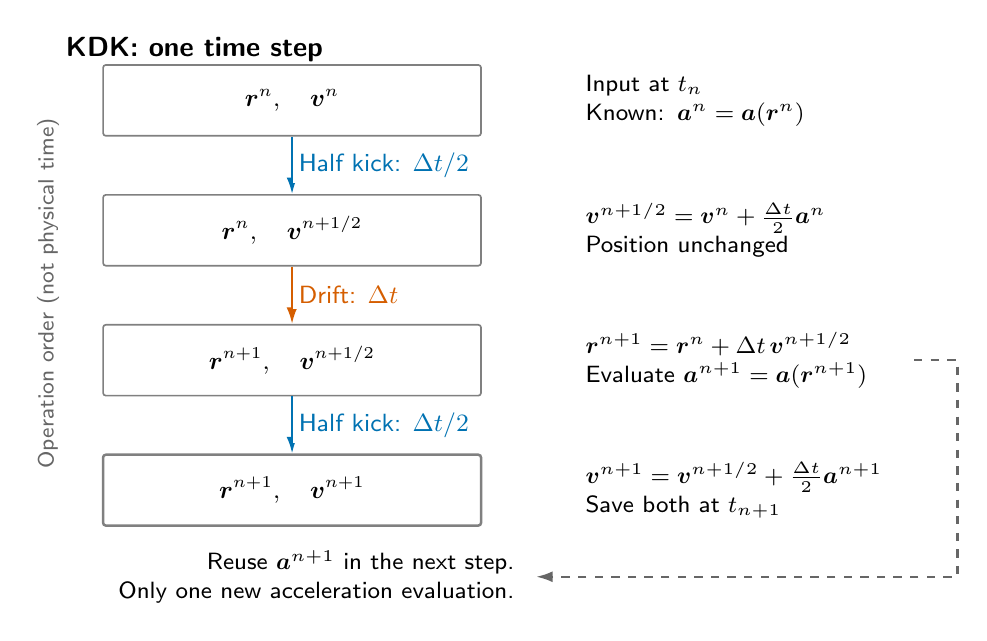
\begin{tikzpicture}[textbook diagram]
  \node[anchor=west,font=\sffamily\bfseries] at (0,0.65) {KDK: one time step};
  \node[state] (in) at (3,0) {$\boldsymbol r^n,\quad\boldsymbol v^n$};
  \node[hint,text width=38mm,anchor=west] at (6.6,0) {Input at $t_n$\\Known: $\boldsymbol a^n=\boldsymbol a(\boldsymbol r^n)$};
  \node[state] (kick) at (3,-1.65) {$\boldsymbol r^n,\quad\boldsymbol v^{n+1/2}$};
  \draw[vector,figblue] (in.south) -- node[right,fill=white,inner sep=2pt] {Half kick: $\Delta t/2$} (kick.north);
  \node[hint,text width=41mm,anchor=west] at (6.6,-1.65) {$\boldsymbol v^{n+1/2}=\boldsymbol v^n+\frac{\Delta t}{2}\boldsymbol a^n$\\Position unchanged};
  \node[state] (drift) at (3,-3.30) {$\boldsymbol r^{n+1},\quad\boldsymbol v^{n+1/2}$};
  \draw[vector,figred] (kick.south) -- node[right,fill=white,inner sep=2pt] {Drift: $\Delta t$} (drift.north);
  \node[hint,text width=41mm,anchor=west] at (6.6,-3.30) {$\boldsymbol r^{n+1}=\boldsymbol r^n+\Delta t\,\boldsymbol v^{n+1/2}$\\Evaluate $\boldsymbol a^{n+1}=\boldsymbol a(\boldsymbol r^{n+1})$};
  \node[state,line width=0.9pt] (out) at (3,-4.95) {$\boldsymbol r^{n+1},\quad\boldsymbol v^{n+1}$};
  \draw[vector,figblue] (drift.south) -- node[right,fill=white,inner sep=2pt] {Half kick: $\Delta t/2$} (out.north);
  \node[hint,text width=41mm,anchor=west] at (6.6,-4.95) {$\boldsymbol v^{n+1}=\boldsymbol v^{n+1/2}+\frac{\Delta t}{2}\boldsymbol a^{n+1}$\\Save both at $t_{n+1}$};
  \draw[vector,figgray,dashed] (10.90,-3.30) -- (11.45,-3.30) -- (11.45,-6.05) -- (6.10,-6.05);
  \node[hint,anchor=east,text width=52mm,align=right] at (5.95,-6.05) {Reuse $\boldsymbol a^{n+1}$ in the next step.\\Only one new acceleration evaluation.};
  \node[rotate=90,small label,text=figgray] at (-0.10,-2.45) {Operation order (not physical time)};
\end{tikzpicture}

\caption{KDKの1ステップで受け渡す位置・速度・加速度。縦方向は計算操作の順序であり、物理時間軸ではありません。最後の半kickを終えた位置と速度を整数時刻の状態として保存し、新しい加速度を次のステップへ引き継ぎます。}
\label{fig:concept-ch1-kdk}
\end{figure}
\FloatBarrier
% END TikZ addition: ch01_kdk

\begin{failbox}{半ステップの速度をそのまま保存しない}
本書の履歴には、同じ整数時刻の位置と速度を保存します。
エネルギーを計算するときに$\rvec^{n+1}$と$\vvec^{n+1/2}$を組み合わせると、異なる時刻の量を使ってしまいます。
最後のkickを終えた$\vvec^{n+1}$を用いてください。
\end{failbox}

\subsection{2次精度になる理由を考える}

位置の更新式に最初のkickを代入すると、
\begin{equation}
\rvec^{n+1}=\rvec^n+\Delta t\vvec^n+\frac{\Delta t^2}{2}\avec^n
\label{eq:ch1-kdk-position-taylor}
\end{equation}
となります。これは位置のTaylor展開の2次までの項と一致します。
Euler法で省いていた、加速度によって軌道が曲がる効果が含まれています。

二つのkickをまとめると、速度は
\begin{equation}
\vvec^{n+1}=\vvec^n+\frac{\Delta t}{2}\left(\avec^n+\avec^{n+1}\right)
\label{eq:ch1-kdk-average-acceleration}
\end{equation}
です。区間の両端の加速度を平均して使います。
滑らかな問題では、この平均による速度更新もTaylor展開の2次までと一致します。
正しい初期値から1ステップだけ進めたときの誤差は$O(\Delta t^3)$です。
同じ有限の時刻まで計算した解の誤差は、十分小さい刻みでは$O(\Delta t^2)$になります。
この意味でleapfrog法は\textbf{2次精度}です。刻みを半分にすると、解の誤差はおよそ$1/4$になると期待できます。

\subsection{時間反転と保存系での性質を理解する}

KDKは、前後が同じ形になるように操作を並べています。
式\eqref{eq:ch1-kdk-last-kick}から逆順に、符号を反転した$-\Delta t$で操作すれば、もとの状態へ戻ります。
固定刻みで、丸め誤差を除けば成り立つこの性質を\textbf{時間反転対称性}と呼びます。

また、本章のような静的なポテンシャル中の運動では、KDKは\textbf{シンプレクティック積分法}です。
これはHamilton系の位相空間の幾何学的な構造を保つ方法という意味です。
本書ではその数学的な証明には立ち入りませんが、\textbf{次数だけでなく、もとの運動方程式の構造を保つことにも価値がある}と理解してください。\cite{simten2007}

シンプレクティックであることは、物理的なエネルギーを毎ステップ厳密に保存することとは違います。
固定刻みで軌道を十分に分解できている滑らかな保存系では、エネルギー誤差が一定の範囲で振動するなど、長時間積分で有利な振る舞いが期待できます。
ただし、刻みが大きすぎる計算まで正しくなるわけではなく、軌道上の位置のずれも蓄積し得ます。
後で、実際の数値解を用いて確かめます。

\subsection{加速度を再利用する}

式\eqref{eq:ch1-kdk-force}で求めた$\avec^{n+1}$は、次のステップの最初のkickでも使います。
この値を保存して渡せば、同じ位置で加速度を計算し直す必要はありません。
最初の$\avec^0$を1回求めた後は、\textbf{1ステップにつき新しい力評価は1回}です。
$N_{\rm step}$ステップでは、全体で$N_{\rm step}+1$回になります。
2回のkickを行うことと、2回の新しい力評価を行うことは同じではありません。

N体計算では、多数の粒子が作る重力場を求める処理が高価です。
加速度を再利用できることは、保存系に適した性質とともに、重力計算でleapfrog法を使う重要な理由です。\cite{simten2007}
Pythonでも、この利点が実際に得られる形で実装します。

\section{4次Runge--Kutta法で運動方程式を解く}
\label{sec:ch1-rk4}

leapfrogは、加速度が位置から決まる重力計算を効率よく進める方法です。
一方、速度に依存する力を扱うときには、状態全体の変化率を使う方法が便利です。
本書では、そのための主要手法としてRK4も本文で学びます。
第6章の動力学的摩擦を含む発展計算で、この方法を使います。

\subsection{1ステップの途中の状態を予測する}

状態の変化を正確に書けば、次の時刻の状態は
\begin{equation}
\yvec(t_n+\Delta t)=\yvec(t_n)+\int_{t_n}^{t_n+\Delta t}\fvec(t,\yvec(t))\,dt
\label{eq:ch1-integral-form}
\end{equation}
です。しかし、積分区間の途中の$\yvec(t)$は、まだ分かっていません。
RK4では途中の状態を順に予測し、そこで右辺を評価します。
高階の時間微分を自分で計算する代わりに、右辺関数$\fvec$を4回使います。\cite{sugiura2009}

\Needspace{17\baselineskip}
本書で使う古典的RK4の4つの段階は、
\begin{align}
\kvec_1 &= \fvec(t_n,\yvec^n),\nonumber\\
\kvec_2 &= \fvec\left(t_n+\frac{\Delta t}{2},\yvec^n+\frac{\Delta t}{2}\kvec_1\right),\nonumber\\
\kvec_3 &= \fvec\left(t_n+\frac{\Delta t}{2},\yvec^n+\frac{\Delta t}{2}\kvec_2\right),\nonumber\\
\kvec_4 &= \fvec\left(t_n+\Delta t,\yvec^n+\Delta t\kvec_3\right)
\label{eq:ch1-rk4-stages}
\end{align}
です。得られた4つの傾きを重み付きで平均し、
\begin{equation}
\boxed{\yvec^{n+1}=\yvec^n+\frac{\Delta t}{6}
\left(\kvec_1+2\kvec_2+2\kvec_3+\kvec_4\right)}
\label{eq:ch1-rk4-update}
\end{equation}
で1ステップを進めます。
ここでは$\kvec_j$を\textbf{状態の時間変化率}として定義し、$\Delta t$を含めていません。

各段階を、物理的な計算として読み直してみましょう。
$\kvec_1$は現在の状態での変化率です。
それを使って半ステップ後の状態を予測し、$\kvec_2$を求めます。
次に$\kvec_2$を使い、\textbf{もう一度、現在の状態$\yvec^n$から}半ステップ後を予測して、$\kvec_3$を求めます。
最後に$\kvec_3$を使って、現在から1ステップ後の状態を予測し、$\kvec_4$を求めます。

$\kvec_2$と$\kvec_3$の評価時刻は同じですが、使う予測状態は異なります。
また、途中で得る状態は、その時刻の確定した数値解ではありません。
1ステップ全体を進めるための、一時的な予測値です。


% BEGIN TikZ addition: ch01_rk4
図\ref{fig:concept-ch1-rk4}では、予測状態と、そこで計算する傾きを分けて示しています。特に第2・第3段階で、時刻は同じでも状態が異なる点を見てください。
\begin{figure}[!htbp]
\centering
% Each predicted state starts from y^n; the arrows show dependencies, not a time partition.
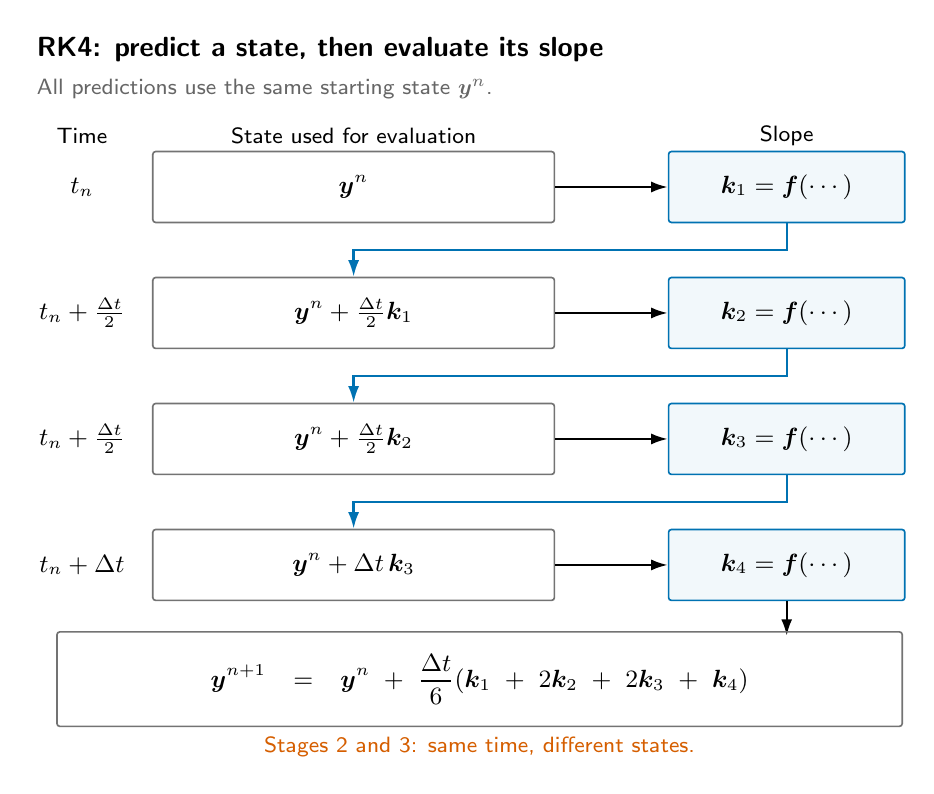
\begin{tikzpicture}[textbook diagram]
  \node[anchor=west,font=\sffamily\bfseries] at (0,0.80) {RK4: predict a state, then evaluate its slope};
  \node[small label,text=figgray,anchor=west] at (0,0.30) {All predictions use the same starting state $\boldsymbol y^n$.};
  \node[small label] at (0.70,-0.30) {Time};
  \node[small label] at (4.15,-0.30) {State used for evaluation};
  \node[small label] at (9.65,-0.30) {Slope};
  \foreach \y/\id in {-0.95/1,-2.55/2,-4.15/3,-5.75/4} {
    \node[draw=black!55,rounded corners=1pt,minimum width=51mm,minimum height=9mm,fill=white] (s\id) at (4.15,\y) {};
    \node[draw=figblue,rounded corners=1pt,minimum width=30mm,minimum height=9mm,fill=figblue!5] (k\id) at (9.65,\y) {$\boldsymbol k_{\id}=\boldsymbol f(\cdots)$};
    \draw[vector] (s\id.east) -- (k\id.west);
  }
  \node at (0.70,-0.95) {$t_n$};
  \node at (0.70,-2.55) {$t_n+\frac{\Delta t}{2}$};
  \node at (0.70,-4.15) {$t_n+\frac{\Delta t}{2}$};
  \node at (0.70,-5.75) {$t_n+\Delta t$};
  \node at (s1) {$\boldsymbol y^n$};
  \node at (s2) {$\boldsymbol y^n+\frac{\Delta t}{2}\boldsymbol k_1$};
  \node at (s3) {$\boldsymbol y^n+\frac{\Delta t}{2}\boldsymbol k_2$};
  \node at (s4) {$\boldsymbol y^n+\Delta t\,\boldsymbol k_3$};
  \foreach \i/\j/\y in {1/2/-1.75,2/3/-3.35,3/4/-4.95} {
    \draw[vector,figblue] (k\i.south) -- (9.65,\y) -- (4.15,\y) -- (s\j.north);
  }
  \node[small label,text=figred] at (5.75,-8.06) {Stages 2 and 3: same time, different states.};
  \draw[vector] (k4.south) -- (9.65,-6.65);
  \node[draw=black!55,rounded corners=1pt,minimum height=12mm,text width=105mm,align=center] at (5.75,-7.20) {$\displaystyle\boldsymbol y^{n+1}=\boldsymbol y^n+\frac{\Delta t}{6}(\boldsymbol k_1+2\boldsymbol k_2+2\boldsymbol k_3+\boldsymbol k_4)$};
\end{tikzpicture}

\caption{RK4の予測状態と傾きの依存関係。各予測は同じ基準状態$\yvec^n$から作ります。$\kvec_2$と$\kvec_3$は評価時刻が同じでも、使う予測状態は異なります。矢印は計算の依存関係で、時間を4等分する図ではありません。}
\label{fig:concept-ch1-rk4}
\end{figure}
\FloatBarrier
% END TikZ addition: ch01_rk4

\subsection{同じ予測状態から位置と速度の変化率を評価する}

重力問題では、状態の上半分が位置、下半分が速度です。
例えば$\kvec_1$は$(\vvec^n,\avec(\rvec^n))$に対応します。
第2段階で右辺を評価する位置と速度は、
\begin{equation}
\rvec_{(2)}=\rvec^n+\frac{\Delta t}{2}\vvec^n,\qquad
\vvec_{(2)}=\vvec^n+\frac{\Delta t}{2}\avec(\rvec^n)
\label{eq:ch1-stage-two}
\end{equation}
です。そして、$\kvec_2$の位置成分の変化率は$\vvec_{(2)}$、速度成分の変化率は$\avec(\rvec_{(2)})$です。
位置だけを予測して、速度は初めのまま使う計算ではありません。

式\eqref{eq:ch1-rk4-update}の係数$1,2,2,1$は、単に「中点を重くする」という思いつきで決めたものではありません。
途中の予測状態の作り方と合わせて、真の解のTaylor展開と4次まで一致するように選ばれています。
一般の場合の次数条件の導出は、数値計算の専門書に譲ります。\cite{sugiura2009}

\subsection{4次精度の意味を確認する}

正確な初期値から1ステップだけ進めたとき、十分滑らかな問題でのRK4の誤差は$O(\Delta t^5)$です。
一方、同じ有限の時間まで多数のステップを積み重ねたときの解の誤差は、十分小さな時間刻みでは$O(\Delta t^4)$になります。
この後者を指して、4次精度と呼びます。

したがって、初期条件と最終時刻を固定して時間刻みを半分にすると、解の誤差はおよそ$1/16$になることが期待できます。
これは誤差の主要な項が$\Delta t^4$に比例する範囲での性質です。
刻みが大きすぎる場合や、丸め誤差が目立つほど小さい場合まで保証する関係ではありません。
また、エネルギーのような特定の量の誤差が、必ず同じべきで変わるとも限りません。

\begin{failbox}{RK4の段階と時間刻みを混同する}
本書の$\kvec_j$に$\Delta t$は含まれません。
別の資料で$\Delta t\fvec$を$\kvec_j$と定義している場合、その更新式をそのまま混ぜると時間刻みを二重に掛けてしまいます。
また、4段階で位置と速度を同じ予測状態から評価することを守ります。
\end{failbox}

\subsection{速度に依存する力も同じ形で扱う}

加速度が$\avec(\rvec,\vvec,t)$となっても、RK4では各段階の位置と速度から右辺を評価します。
状態ベクトルと4段階の更新式を変更する必要はありません。
一方、ここまでのKDKでは、位置を固定すればkickの間の加速度も固定できることを使いました。
速度依存力ではkickの間にも加速度が変わるので、同じ陽的な更新をそのまま使うことはできません。

これは「leapfrogの考え方では速度依存力を一切扱えない」「RK4だけが使える」という意味ではありません。
分割法や陰的な速度更新を組み合わせる方法もありますが、本書では複数の方法を追加せず、RK4へ切り替えます。
RK4を採用する理由は、速度依存力を含む運動方程式を、学習済みの同じ枠組みで扱えることです。

\begin{notebox}{本文で詳しく扱わない時間積分法}
\textbf{RK2}は、少ない段階で2次精度を得るRunge--Kutta法です。
\textbf{適応刻みRK法}は、推定誤差に応じて時間刻みを変えます。
\textbf{Bulirsch--Stoer法}は、複数の刻みで計算した解から外挿を行う方法です。
また、kickとdriftの組合せから\textbf{高次のシンプレクティック法}を作ることもできます。
本書ではKDKとRK4の基本的な性質に集中するため、高次の方法の詳細は数値計算法の参考図書に譲ります。高次のシンプレクティック法については文献\cite{simten2007}も参照してください。
\end{notebox}

\section{Pythonで軌道を計算する}
\label{sec:ch1-python}

\subsection{状態を配列へ対応させる}

まず、\verb|import numpy as np|と\verb|import matplotlib.pyplot as plt|を実行します。
本章では1個の粒子でも、位置と速度をそれぞれ形が\verb|(1, 2)|の配列に入れます。
最初の軸が粒子、2番目の軸が$x,y$の成分です。
後の章で粒子数を$N$へ増やしても、\verb|(N, 2)|という同じ約束を使います。

次のコードで、単位変換、初期条件、計算時間を設定します。
leapfrogでは\verb|pos|と\verb|vel|を分けて更新します。
RK4では\verb|np.column_stack|で位置と速度を横に並べ、
\verb|[x, y, vx, vy]|を1行に持つ形\verb|(1, 4)|の\verb|state|を使います。
これはデータの持ち方の違いであり、計算する運動方程式は同じです。
\inputcode{chap01/parameters}

\verb|np.array([[r0, 0.0]])|の角括弧が二重なのは、粒子の行と成分の列を作るためです。
\verb|pos0[0]|で最初の粒子の位置ベクトルを取り出せます。
式\eqref{eq:ch1-acceleration-components}を、まず1粒子の成分のまま計算します。
\inputcode{chap01/acceleration-scalar}
初期位置では、出力される$a_x$は$\chonevalAcceleration\unit{kpc\,Gyr^{-2}}$、$a_y$は0です。
原点へ向かう加速度になっていることを確認してください。

\subsection{加速度関数と右辺関数を分ける}

今計算した式を、位置から加速度を返す関数にします。
入力と返り値は、どちらも形が\verb|(1, 2)|です。
この関数は本章の1粒子専用で、多数粒子への一般化は第4章で行います。
\inputcode{chap01/acceleration-kepler}

leapfrogには、この加速度関数を渡します。
Euler法とRK4には、位置と速度をまとめた状態の変化率を返す関数を渡します。
同じ加速度関数を使い、式\eqref{eq:ch1-state-ode}の右辺を組み立てます。
\inputcode{chap01/rhs-kepler}
\verb|state[:, :2]|が位置、\verb|state[:, 2:]|が速度です。
右辺の先頭2成分は速度、後半2成分は加速度です。
\verb|t|は本章では使いませんが、時間依存する問題にも使えるように残します。

\subsection{KDKの1ステップを実装する}

式\eqref{eq:ch1-kdk-first-kick}から式\eqref{eq:ch1-kdk-last-kick}までを、その順に書きます。
引数\verb|acc|は、現在の\verb|pos|に対応する計算済みの加速度です。
\inputcode{chap01/leapfrog-step}

\verb|vel_half|は中間速度、\verb|pos_new|と\verb|vel_new|は次の整数時刻の状態です。
返り値の\verb|acc_new|を次の呼び出しへ渡します。
関数内部の\verb|acceleration(...)|は1回だけです。
入力配列を直接上書きせず、新しい配列を返すため、比較計算でも初期値を保てます。

\textbf{確認：} 最後のkickで\verb|acc_new|ではなく古い\verb|acc|を使うと、
新しい位置で変化した重力を反映できません。
また、\verb|acc|と\verb|pos|の対応がずれると、意図したKDKではなくなります。

\subsection{Euler法とRK4の1ステップを実装する}

Euler法は、状態全体に更新前の変化率を掛けるだけです。
\inputcode{chap01/euler-step}
RK4は、式\eqref{eq:ch1-rk4-stages}と式\eqref{eq:ch1-rk4-update}を順に実装します。
\inputcode{chap01/rk4-step}
\verb|state + 0.5 * dt * k1|には、予測位置と予測速度が一緒に入ります。
RK4の段階全体で同じ予測状態を使う点は、位置と速度を分けて更新するKDKとの違いです。

\subsection{更新を繰り返して履歴を残す}

KDKでは、最初の加速度をループの外で1回だけ計算します。
その後は、位置・速度・加速度を受け取り、次のステップへ渡します。
\inputcode{chap01/integrate-leapfrog}

\verb|prepare_history|は、正のステップ数、有限の最終時刻、初期配列の形を確認する補助関数です。
初期状態のコピー、$\Delta t=t_{\rm end}/N_{\rm step}$、$t_n=n\Delta t$、保存用配列を用意します。
その実装はNotebookに示します。
\verb|history|の形は\verb|(n_steps + 1, 1, 4)|です。
初期状態を含むので、出力数はステップ数より1つ多くなります。
KDKの履歴にも、\textbf{位置と最後のkick後の速度}を同じ行へ保存します。

Euler法とRK4では、一般の右辺と1ステップ関数を渡して計算します。
\inputcode{chap01/integrate}

同じ初期条件から、3つの方法を実行します。
本章では変数\verb|history|に標準法のleapfrogの結果を入れ、RK4とEuler法には別の変数を使います。
\inputcode{chap01/run-orbit}

\section{軌道を図とアニメーションで見る}
\label{sec:ch1-visualization}

円軌道を初期条件に選んだので、時刻$t$における正解は、初期条件から独立に計算できます。
角速度$\Omega$を使うと、位置と速度は
\begin{align}
\rvec_{\rm exact}(t)&=r_0\bigl(\cos\Omega t,\,\sin\Omega t\bigr),\nonumber\\
\vvec_{\rm exact}(t)&=r_0\Omega\bigl(-\sin\Omega t,\,\cos\Omega t\bigr)
\label{eq:ch1-exact-circle}
\end{align}
です。数値解と解析解を、必ず\textbf{同じ時刻}で比べます。
単にどちらも円を描いているだけでは、1周する速さが正しいかは分かりません。

解析解を計算するコードは次のようになります。
ここで\verb|pos_history|の最初の軸は、粒子数ではなく、保存した時刻を表しています。
\inputcode{chap01/exact-circle}

図\ref{fig:ch1-orbit}は、標準の200ステップで計算したleapfrogの軌道です。
$0,T/4,T/2,3T/4$の位置も示しました。
解析解と数値解は、この図の大きさではほぼ重なります。
図を描くときは\verb|ax.set_aspect("equal")|を使い、縦横で同じ距離が同じ長さに見えるようにします。
そうしないと、円を楕円のように表示してしまいます。

\begin{figure}[!htbp]
\centering
\includegraphics[width=0.66\linewidth]{\figpath{ch01_orbit}}
\caption{中心質量の周りを回る1粒子の軌道。標準条件のleapfrog（KDK）を青実線、解析的な円を灰色破線で示します。
四角は指定した時刻の数値解、星印は固定した中心質量です。計算は反時計回りです。}
\label{fig:ch1-orbit}
\end{figure}

描画の中心部分を次に示します。\verb|save_figure|はNotebookに用意した保存用関数で、同じ図をPDFとPNGに保存して表示します。
\inputcode{chap01/plot-orbit}

同じ条件でEuler法を使った結果を、図\ref{fig:ch1-method-comparison}に重ねました。
本来は1周期で初期位置へ戻りますが、Euler法では軌道が外側へずれ、1周期後の位置も大きく異なります。
これは別の初期速度を与えた結果ではなく、\textbf{同じ運動方程式と同じ初期条件を、異なる近似で時間積分した結果}です。

\begin{figure}[!htbp]
\centering
\includegraphics[width=0.67\linewidth]{\figpath{ch01_method_comparison}}
\caption{同じ時間刻み$\Delta t=T/200$でのEuler法・leapfrog・RK4の比較。計算時間は解析的な1周期です。
朱色の一点鎖線がEuler法、青実線がleapfrog、緑破線がRK4、灰色点線が解析解です。
同じステップ数でも力評価回数は異なり、leapfrogとRK4の軌道はこの縮尺ではほぼ重なります。}
\label{fig:ch1-method-comparison}
\end{figure}

\paragraph{アニメーションと静止画}
Notebookでは、保存済みの\verb|history|から粒子の位置を順に読み、アニメーションを作ります。
表示のたびに運動方程式を解き直す必要はありません。
再生間隔を決める\verb|interval|は画面上の時間であり、物理的な時間刻み\verb|dt|ではありません。
再生速度を変えても計算した軌道は変わりません。
本文では図\ref{fig:ch1-orbit}のように重要な時刻の位置を静止画としても残し、動画を見なくても結果が分かるようにします。

\section{エネルギーと角運動量を確かめる}
\label{sec:ch1-conservation}

\subsection{このモデルで保存される量を確認する}

軌道の見た目だけでは、小さな誤差は分かりません。
そこで、ゼミで学んだ保存量を数値解から計算します。
中心質量は固定され、ポテンシャルは時間に依存しません。
粒子の単位質量当たりのエネルギーは
\begin{equation}
\varepsilon=\frac12(v_x^2+v_y^2)-\frac{\mu}{r}
\label{eq:ch1-specific-energy}
\end{equation}
です。速度変化による運動エネルギーの変化率と、位置変化によるポテンシャルエネルギーの変化率が打ち消し合い、
\begin{equation}
\frac{d\varepsilon}{dt}=\vvec\cdot\avec+
\frac{\mu}{r^3}\rvec\cdot\vvec=0
\label{eq:ch1-energy-conservation}
\end{equation}
となります。

また、重力は原点からの位置ベクトルと平行で、原点の周りのトルクは0です。
運動面に垂直な単位質量当たりの角運動量は
\begin{equation}
\ell_z=xv_y-yv_x,\qquad
\frac{d\ell_z}{dt}=xa_y-ya_x=0
\label{eq:ch1-specific-angular}
\end{equation}
となります。ここで確認するのは粒子の\textbf{比}エネルギーと\textbf{比}角運動量であり、粒子の質量$m$は掛けません。
これらは、中心力中の軌道を理解する基本的な保存量です。\cite{ryden2025}

円軌道の初期値では、
\begin{equation}
\varepsilon_0=-\frac{\mu}{2r_0},\qquad
\ell_{z,0}=r_0v_c=\sqrt{\mu r_0}
\label{eq:ch1-initial-invariants}
\end{equation}
です。負のエネルギーは、この粒子が中心質量に束縛されていることを表します。
今回は$\varepsilon_0$も$\ell_{z,0}$も0ではないので、それぞれの初期値の絶対値で誤差を規格化できます。

\subsection{数値解から保存量を計算する}

履歴から位置と速度を取り出し、式\eqref{eq:ch1-specific-energy}と式\eqref{eq:ch1-specific-angular}を評価します。
\texttt{np.sum(...,}\allowbreak\ \texttt{axis=1)}は、ここでは各時刻の2成分を足す操作です。
例えば\texttt{np.sum(vel**2,}\allowbreak\ \texttt{axis=1)}は、各時刻の$v_x^2+v_y^2$を返します。
\inputcode{chap01/diagnostics}

時刻$t_n$での誤差の大きさを、
\begin{equation}
e_\varepsilon^n=\frac{|\varepsilon^n-\varepsilon^0|}{|\varepsilon^0|},\qquad
e_\ell^n=\frac{|\ell_z^n-\ell_z^0|}{|\ell_z^0|}
\label{eq:ch1-conservation-errors}
\end{equation}
と定義します。保存した全時刻での最大値を、それぞれ$e_\varepsilon,e_\ell$とします。図\ref{fig:ch1-energy-error}は、エネルギー誤差を時間の関数として示したものです。
$t=0$では定義上誤差が0です。対数軸では0を表示できないため、その点だけを描いていません。
保存した数値を、小さな正数へ置き換えているわけではありません。

\begin{figure}[!htbp]
\centering
\includegraphics[width=0.79\linewidth]{\figpath{ch01_energy_error}}
\caption{標準条件でのエネルギーの相対誤差。各方法の初期値からの変化の絶対値を示しています。
縦軸は対数です。Euler法、leapfrog、RK4を比べています。leapfrogもRK4もエネルギーを厳密に保存するわけではありません。}
\label{fig:ch1-energy-error}
\end{figure}

標準条件の誤差を表\ref{tab:ch1-base-errors}にまとめました。
位置の誤差$e_r$は、解析解との位置の差を初期半径で割った最大値です。次節で詳しく定義します。
\begin{table}[!htbp]
\centering
\caption{同じ1周期・200ステップでの比較。$e_r$は最大位置誤差、$e_\varepsilon$と$e_\ell$は保存量の最大相対誤差です。
本章の実行結果であり、末尾の桁は実行環境で多少変わります。}
\label{tab:ch1-base-errors}
\small
\begin{tabular}{lrrrr}\toprule
方法 & 力評価回数 & $e_r$ & $e_\varepsilon$ & $e_\ell$ \\
\midrule
Euler & 200 & $1.43\times 10^{0}$ & $2.31\times 10^{-1}$ & $1.38\times 10^{-1}$ \\
Leapfrog (KDK) & 201 & $2.16\times 10^{-3}$ & $2.43\times 10^{-7}$ & $6.43\times 10^{-16}$ \\
RK4 & 800 & $1.65\times 10^{-7}$ & $5.34\times 10^{-9}$ & $2.67\times 10^{-9}$ \\
\bottomrule\end{tabular}

\end{table}

leapfrogのエネルギー誤差は約$\choneerrLfEnergy$です。
一方、角運動量のずれは約$\choneerrLfAngular$で、丸め誤差程度にとどまります。
これは、中心力によるkickとdriftの各操作が、角運動量を保つためです。
例えばkickでは$\rvec\times\avec=0$なので、速度に$h\avec$を加えても$\rvec\times\vvec$は変わりません。
driftでも、位置へ$h\vvec$を加えた寄与は$h\vvec\times\vvec=0$です。
この説明は本章の中心力についてのもので、任意の外力に角運動量保存を保証するものではありません。

RK4の最大相対エネルギー誤差は$\choneerrRkEnergy$、角運動量誤差は$\choneerrRkAngular$でした。
短時間の位置とエネルギーの精度は非常に高い一方、エネルギーや角運動量を厳密に保存する手法ではありません。\cite{sugiura2009}
また、どの方法でも、保存量のずれが小さいことだけで軌道上の位置が正しいとは判断できません。
次節では、解析解に対する位置ベクトルの誤差を直接調べます。

\begin{failbox}{保存量はモデルを見て選ぶ}
本章では、静的な中心重力場なのでエネルギーと角運動量を確認できます。
後の章のように、重力場が時間変化する場合や摩擦がある場合には、粒子のエネルギーは一般に保存しません。
「エネルギーが変わったからコードが間違っている」と決める前に、計算したモデルで何が保存されるかを確認します。
\end{failbox}

\section{時間刻みを変えて誤差を調べる}
\label{sec:ch1-convergence}

\subsection{位置ベクトルの誤差を測る}

時間刻みの影響を分けて調べるため、中心質量、初期位置、初期速度、最終時刻$T$を固定します。
変えるのはステップ数だけです。ステップ数を2倍にすると、時間刻みは半分になります。
数値解と解析解を同じ時刻で比較し、位置の差を$r_0$で規格化します。
保存した全時刻での最大値を
\begin{equation}
e_r=\max_{0\le n\le N_{\rm step}}
\frac{|\rvec^n-\rvec_{\rm exact}(t_n)|}{r_0}
\label{eq:ch1-position-error}
\end{equation}
と定義します。
これは半径の差だけではなく、位置\textbf{ベクトル}の差です。
円に沿っていても回転の速さがずれていれば、誤差に現れます。
同様に、式\eqref{eq:ch1-conservation-errors}の最大値を$e_\varepsilon,e_\ell$とします。
\inputcode{chap01/error-metrics}

同じステップ数でleapfrogとRK4を計算し、その結果を表にまとめます。
\inputcode{chap01/convergence}
\begin{table}[!htbp]
\centering
\caption{時間刻みと最大位置誤差。すべて同じ初期条件から1周期$T$まで計算しています。
$p_r$は一つ前の行との誤差比から求めた見かけの次数です。
保存量の誤差も、配布するCSVに保存しています。}
\label{tab:ch1-convergence}
\small
\begin{tabular}{rrrrrr}\toprule
$N_{\rm step}$ & $\Delta t\ [\mathrm{Myr}]$ & $e_r$ (KDK) & $p_r$ & $e_r$ (RK4) & $p_r$ \\
\midrule
20 & 14.8121 & $2.09\times 10^{-1}$ & --- & $3.91\times 10^{-3}$ & --- \\
40 & 7.4060 & $5.35\times 10^{-2}$ & 1.967 & $1.66\times 10^{-4}$ & 4.557 \\
80 & 3.7030 & $1.35\times 10^{-2}$ & 1.990 & $7.93\times 10^{-6}$ & 4.387 \\
160 & 1.8515 & $3.37\times 10^{-3}$ & 1.998 & $4.19\times 10^{-7}$ & 4.242 \\
320 & 0.9258 & $8.44\times 10^{-4}$ & 1.999 & $2.40\times 10^{-8}$ & 4.129 \\
\bottomrule\end{tabular}

\end{table}

\subsection{2次精度と4次精度を確認する}

刻みを半分にした二つの計算から、見かけの次数を
\begin{equation}
p_r=\frac{\log\bigl[e_r(\Delta t)/e_r(\Delta t/2)\bigr]}{\log 2}
\label{eq:ch1-observed-order}
\end{equation}
で求めます。leapfrogでは2へ、RK4では4へ近づくと期待できます。
表\ref{tab:ch1-convergence}の最も細かい側では、それぞれ$\chonevalLfOrder$と$\chonevalRkOrder$です。
図\ref{fig:ch1-convergence}では、同じ数値を両対数の図にしています。
点線と一点鎖線は、それぞれ傾き2と4の参照線です。

\begin{figure}[!htbp]
\centering
\includegraphics[width=0.80\linewidth]{\figpath{ch01_convergence}}
\caption{時間刻みと最大位置誤差の関係。青丸がleapfrog、緑四角がRK4です。
参照線は各方法の最も細かい刻みの実測点を通り、傾きを2または4に固定した線です。
データに当てはめて求めた線ではありません。}
\label{fig:ch1-convergence}
\end{figure}

粗い刻みでは高次の誤差項も影響するため、見かけの次数は2や4から離れます。
一方、極端に細かい刻みでは、浮動小数点演算の丸め誤差が目立つことがあります。
期待した誤差比は、刻みが十分小さく、かつ丸め誤差が支配しない範囲で確認します。

円軌道では、エネルギーなど特定の量の誤差に打ち消しが生じる場合があります。
その量だけから「leapfrogは4次」「RK4は5次」と判断してはいけません。
本章では、同じ時刻の解析解に対する位置のずれを、解法の次数を確認する指標にしました。

\section{計算コストと長時間の振る舞いを比較する}
\label{sec:ch1-cost-long-time}

\subsection{力評価回数をそろえる}

同じ時間刻みで比べれば、RK4の方が小さい位置誤差を与えました。
ただし、RK4は1ステップで右辺を4回評価し、各評価で重力を計算します。
キャッシュ付きKDKは、最初の1回を除けば新しい重力評価が1回だけです。
$N_{\rm step}$ステップの力評価回数は
\begin{equation}
N_{\rm force}=\begin{cases}
N_{\rm step} & \text{Euler},\\
N_{\rm step}+1 & \text{leapfrog（KDK）},\\
4N_{\rm step} & \text{RK4}
\end{cases}
\label{eq:ch1-force-counts}
\end{equation}
です。ここでは時間積分のための力評価だけを数え、保存量の計算や描画は含めません。
200ステップの場合の200回、201回、800回という値は、配布コードの独立試験でも関数の呼び出し数から確認しています。

力評価回数を800回にそろえる比較も行います。
KDKは初回の1回が必要なので799ステップ、RK4は200ステップです。
いずれも同じ1周期$T$まで進めます。
\inputcode{chap01/equal-cost}
\begin{table}[!htbp]
\centering
\caption{力評価回数を800回にそろえた1周期の比較。時間刻みは同じではありません。
$e_r$は最大位置誤差、$e_\varepsilon$は最大相対エネルギー誤差です。}
\label{tab:ch1-cost}
\small
\begin{tabular}{lrrrr}\toprule
方法 & $N_{\rm step}$ & 力評価回数 & $e_r$ & $e_\varepsilon$ \\
\midrule
Leapfrog (KDK) & 799 & 800 & $1.35\times 10^{-4}$ & $9.56\times 10^{-10}$ \\
RK4 & 200 & 800 & $1.65\times 10^{-7}$ & $5.34\times 10^{-9}$ \\
\bottomrule\end{tabular}

\end{table}

この滑らかな円軌道の短時間計算では、力評価回数をそろえてもRK4の位置誤差の方が小さくなりました。
したがって、\textbf{力評価が少ないから、常にleapfrogの方が高精度になるわけではありません。}
必要な精度、計算する時間の長さ、保存系としての性質を合わせて考えます。

直接N体計算では、1回の重力評価に多数の粒子対の計算が含まれます。
粒子数を$N$とすると、直接和の計算量は$O(N^2)$です。
本書のテスト粒子モデルは少数のポテンシャルから力を受けるので$O(N)$ですが、どちらでも力評価の節約には意味があります。
ただし、実行時間には配列の作成やPythonの処理も含まれます。
力評価回数だけから「実行時間が必ず4倍違う」とは言えません。
Notebookには実行時間を測る例も用意し、環境ごとに確かめます。

\subsection{同じ円軌道を100周期まで進める}

次に、円軌道を長く追跡します。
初期条件は同じですが、この実験だけ時間刻みを$\Delta t=T/100$、最終時刻を$100T$とします。
短時間の表と混同しないよう、条件の違いを明示しておきます。
両方法とも10000ステップで、力評価回数はKDKが10001回、RK4が40000回です。

エネルギーが一方向へずれるのか、増減を繰り返すのかを見るため、
ここでは絶対値ではなく、\textbf{符号付き}の差$[\varepsilon(t)-\varepsilon(0)]/|\varepsilon(0)|$を描きます。
\inputcode{chap01/long-time}
\begin{figure}[!htbp]
\centering
\includegraphics[width=0.81\linewidth]{\figpath{ch01_long_time_energy}}
\caption{円軌道の100周期積分。両方法とも$\Delta t=T/100$です。
青実線がKDK、緑破線がRK4です。KDKの細かい振動は、この縮尺では帯のように見えます。
同じ時間刻みでの比較であり、同じ力評価回数での比較ではありません。}
\label{fig:ch1-long-time-energy}
\end{figure}

この条件では、KDKのエネルギー差は0付近から約$\chonelongLfMax$までの範囲で振動しました。
RK4の差は負の向きへ蓄積し、$100T$で約$\chonelongRkFinal$となりました。
これは本章の実行結果であり、任意の軌道や刻みで同じ数値や符号になるという主張ではありません。

静的な滑らかな保存系を固定刻みで解くとき、leapfrogの構造を保つ性質は、このような長時間の誤差の振る舞いに利点を持ちます。\cite{simten2007}
ただし、エネルギー差が狭い範囲に収まっていても、軌道の位相が正確とは限りません。
精度の確認には、保存量と位置の誤差を併用します。

\subsection{本書での使い分けを考える}

第2章から第5章までの重力計算では、leapfrog（KDK）を標準とします。
計算コストを抑えながら重力系を追跡する方法として、実装を繰り返し使います。
RK4は、一般の常微分方程式を解くもう一つの主要手法として理解し、第6章の速度依存力を含む発展問題で用います。

そこではChandrasekharの動力学的摩擦を、質量をもつ衛星銀河・銀河中心の運動へ加えます。
質量ゼロの恒星テスト粒子そのものに摩擦を掛けるわけではありません。
本章末の速度比例抵抗は、その前に速度依存力を扱うための小さな練習です。
\textbf{手法は次数の高さだけでなく、方程式の形、必要な精度、計算コストに応じて選びます。}

\Needspace{14\baselineskip}
\section{本章のまとめ}
\label{sec:ch1-summary}

本章では、固定した中心質量の周りを動く1個の粒子を計算しました。
位置と速度を変数として持つと、Newtonの運動方程式を1階の連立常微分方程式として扱えます。
加速度を計算する部分と時間を進める部分を分けることで、同じ問題に異なる積分法を適用できました。

Euler法で時間を刻む考え方を確認した後、重力計算の標準法としてleapfrog（KDK）を実装しました。
半kick、drift、半kickという順序、整数時刻にそろえた速度の保存、加速度の再利用が重要です。
一般の常微分方程式へ進むため、RK4の4段階も学びました。
RK4は、速度依存力を含む発展問題で再利用します。

両者を、軌道の見た目、解析解との位置の差、エネルギー、角運動量、時間刻み、力評価回数から比較しました。
leapfrogは2次、RK4は4次ですが、次数だけで優劣は決まりません。
長時間の保存特性と、必要な精度を得るための計算コストも判断材料です。
\textbf{計算が最後まで動いたことと、目的に必要な精度が得られたことは同じではありません。}
次の章ではleapfrogを使い、2つの天体が互いの重力で動く問題へ進みます。

\chapterexercises
\paragraph{演習1.1　確認：初期値と単位}
表\ref{tab:ch1-parameters}の条件から、$v_c,T,\varepsilon_0,\ell_{z,0}$を計算してください。
$v_c$は$\mathrm{km\,s^{-1}}$と$\mathrm{kpc\,Gyr^{-1}}$の両方で示し、保存量にも単位を付けてください。

\paragraph{演習1.2　確認：KDKの更新と力評価}
KDKの3段階を式で書き、各kickで使う加速度がどの位置に対応するか説明してください。
200ステップの力評価回数を求めてください。
また、$\rvec^{n+1}$と$\vvec^{n+1/2}$からエネルギーを計算する場合の問題点を説明してください。

\paragraph{演習1.3　確認：RK4の中間状態}
$\kvec_2$と$\kvec_3$の評価時刻と予測状態を、それぞれ式で書いてください。
$\kvec_2$を求めるとき、位置成分の時間変化率に$\vvec^n$をそのまま使うと、何が間違うでしょうか。

\paragraph{演習1.4　応用：ステップ数の変更}
初期条件と最終時刻$T$を固定し、$N_{\rm step}=50,100,200$でleapfrogとRK4を実行してください。
最大位置誤差$e_r$を求め、ステップ数を2倍にした誤差比を調べてください。
軌道の図だけで精度を区別できるかも考えてください。

\paragraph{演習1.5　応用：回転方向の変更}
初期条件の$v_y$だけを$-v_c$へ変え、leapfrogで同じ時間まで積分してください。
軌道、エネルギー、角運動量はどのように変わるでしょうか。
数値解が$x$軸について鏡映した関係になるかを確認してください。

\paragraph{演習1.6　応用：同じ計算コストでの比較}
時間積分の力評価を両方とも800回にそろえ、1周期を計算してください。
両方法のステップ数、時間刻み、位置誤差を比べてください。
同じ刻みでの比較とは、何をそろえ、何を変えている点が違いますか。

\paragraph{演習1.7　発展：速度に依存する力}
重力加速度に速度比例抵抗$-\gamma\vvec$を追加し、$\gamma=0.05/T$として、400ステップで1周期分の時間まで積分してください。
右辺関数だけを変更し、RK4の関数はそのまま使います。
このモデルでは
\begin{equation}
\frac{d\varepsilon}{dt}=-\gamma v^2
\label{eq:ch1-linear-drag-work}
\end{equation}
となります。エネルギー変化の向きは、この式と整合するでしょうか。
この抵抗力は速度依存力の練習用であり、Chandrasekharの動力学的摩擦公式ではありません。

\newcommand{\chtwovalVc}{179.601851}
\newcommand{\chtwovalVcInt}{183.680998}
\newcommand{\chtwovalTc}{0.684141}
\newcommand{\chtwovalDt}{0.684141}
\newcommand{\chtwovalMu}{6.74774\times 10^{5}}
\newcommand{\chtwovalMred}{3.33333\times 10^{10}}
\newcommand{\chtwovalEllA}{14.705882}
\newcommand{\chtwovalEllP}{0.431357}
\newcommand{\chtwovalEllRp}{9.411765}
\newcommand{\chtwovalEllMin}{9.412506}
\newcommand{\chtwovalEllErrE}{5.72\times 10^{-5}}
\newcommand{\chtwovalOrderC}{1.9999}
\newcommand{\chtwovalOrderEll}{1.9995}
\newcommand{\chtwovalEncMin}{8.000330}
\newcommand{\chtwovalEncTime}{0.3145}
\newcommand{\chtwovalEncVr}{-136.518}
\newcommand{\chtwovalEncVt}{53.547}
\newcommand{\chtwovalBoostRel}{4.87\times 10^{-14}}
\newcommand{\chtwovalBoostCm}{4.06\times 10^{-15}}
\newcommand{\chtwovalReverseR}{2.90\times 10^{-14}}
\newcommand{\chtwovalReverseV}{2.86\times 10^{-14}}
\newcommand{\chtwovalHyperD}{130.721}
\newcommand{\chtwovalEllPeriods}{1.586}
\newcommand{\chtwovalInitialXone}{-6.666667}
\newcommand{\chtwovalInitialXtwo}{13.333333}
\newcommand{\chtwovalInitialVone}{-59.867284}
\newcommand{\chtwovalInitialVtwo}{119.734568}
\newcommand{\chtwovalRadiusSeriesOne}{10.000000,6.666667,1.818182}
\newcommand{\chtwovalRadiusSeriesTwo}{10.000000,13.333333,18.181818}

\chapter{2体問題を計算する}
\label{chap:two-body}
第1章では、原点に固定した中心質量の周りを動く1個の粒子を計算しました。この章では、二つの天体が互いに重力を及ぼし、両方とも動く問題へ進みます。時間積分には、前章で学んだleapfrog法のkick--drift--kick（KDK）形式を使います。新しく作る中心的な部分は、二つの位置から両方の加速度を求める処理と、重心・相対運動を用いた初期条件です。

ゼミで学んだ2体問題を、長い解析解の導出からやり直すことはしません。計算に必要な式を短く整理し、円・楕円・放物線の軌道を作ります。その後、全エネルギー、全角運動量、全運動量、重心運動を確かめます。最後に、指定した近点距離へ向かう接近軌道を作り、第5章の銀河相互作用へ向けた準備をします。

\begin{goalbox}[この章で学ぶこと]
\begin{itemize}
\item 2天体の重力加速度を、作用・反作用を保つ形で計算できます。
\item 重心運動と相対運動を区別し、質量比に応じた初期位置・速度を設定できます。
\item 第1章のKDKを使って、両天体を同じ時刻へ更新できます。
\item 初期速度を変えて円・楕円・放物線を作り、解析的な軌道の性質と比較できます。
\item 保存量と位置の誤差を使い、時間刻みの影響を確認できます。
\end{itemize}
\end{goalbox}

\section{一方を固定する近似を外す}
\label{sec:ch2-model}
\subsection{本章で計算する対象を整理する}
質量$M_1,M_2$の2天体を考えます。両方に有限の質量があり、互いに重力を及ぼします。外部からの力はなく、質量は時間によらず一定です。慣性系の$x$--$y$平面内で運動を追跡します。

本章では、各天体を大きさのない\textbf{点質量}として扱います。これは、2体問題の軌道と保存量を確かめるための練習モデルです。後の章で使う銀河の有限サイズ、円盤のテスト粒子、動力学的摩擦は、まだ入れません。とくに、2天体が同じ位置へ衝突する初期条件は扱いません。

第1章では、中心天体が動かないと近似しました。今回はその近似を外すので、重い天体も動きます。質量が同じなら二つは対称に動き、質量が異なれば、重い天体ほど重心の近くを小さく動きます。まずは質量を異ならせ、この違いを見える形にします。

\subsection{位置と相対位置を区別する}
天体$k=1,2$の位置と速度を$\Rvec_k,\Vvec_k$と書きます。大文字を使うのは、後の章の銀河中心と記法をそろえるためです。天体1から天体2へ向かう相対位置と、その変化率を
\begin{equation}
\Dvec=\Rvec_2-\Rvec_1,\qquad D=|\Dvec|,\qquad
\Uvec=\Vvec_2-\Vvec_1=\frac{d\Dvec}{dt}
\label{eq:ch2-relative-def}
\end{equation}
と定義します。$D$は\textbf{2天体の間の距離}です。それぞれの天体から原点までの距離とは、一般に一致しません。

位置の原点は、どちらかの天体へ毎回移動させるのではなく、まず一つの慣性系に固定します。天体1を原点に置いたような相対軌道の図は、計算後に式\eqref{eq:ch2-relative-def}で座標を引き算して作ります。座標を変換して表示することと、一方の天体の運動を無視することは別です。

\section{二つの加速度を同じ位置から求める}
\label{sec:ch2-force}
\subsection{力と加速度の違いを確認する}
天体1は天体2へ、天体2は天体1へ引かれます。式\eqref{eq:ch2-relative-def}の向きを使うと、Newtonの運動方程式は
\begin{align}
M_1\frac{d\Vvec_1}{dt}&=+GM_1M_2\frac{\Dvec}{D^3},\label{eq:ch2-force1}\\
M_2\frac{d\Vvec_2}{dt}&=-GM_1M_2\frac{\Dvec}{D^3}.\label{eq:ch2-force2}
\end{align}
両辺をそれぞれの質量で割り、加速度$\boldsymbol A_k=d\Vvec_k/dt$を求めると、
\begin{equation}
\boldsymbol A_1=+GM_2\frac{\Dvec}{D^3},\qquad
\boldsymbol A_2=-GM_1\frac{\Dvec}{D^3}
\label{eq:ch2-acceleration}
\end{equation}
となります。自分自身の質量は消えますが、重力を作る相手の質量は残ります。両方とも同じ時刻の$\Rvec_1,\Rvec_2$から計算します。これらはRydenの2体問題で用いる運動方程式に対応します。\cite{ryden2025}

作用・反作用の関係は
\begin{equation}
M_1\boldsymbol A_1+M_2\boldsymbol A_2=\boldsymbol 0
\label{eq:ch2-force-balance}
\end{equation}
です。$M_1\ne M_2$なら、$\boldsymbol A_1=-\boldsymbol A_2$ではありません。例えば$M_1=2M_2$なら、天体2の加速度の大きさは天体1の2倍です。

\subsection{成分で確かめてから関数にする}
$\Dvec=(d_x,d_y)$、$D^2=d_x^2+d_y^2$と書けば、例えば$x$成分は
\begin{equation}
A_{1x}=\frac{GM_2d_x}{(d_x^2+d_y^2)^{3/2}},\qquad
A_{2x}=-\frac{GM_1d_x}{(d_x^2+d_y^2)^{3/2}}
\label{eq:ch2-acceleration-components}
\end{equation}
です。$y$成分も分子の$d_x$を$d_y$へ替えるだけです。天体2が天体1の右側にあれば、$A_{1x}>0$、$A_{2x}<0$となります。この単純な配置で符号を確認してから、軌道を計算します。

実装では$G\Dvec/D^3$を一度だけ求め、それに相手の質量と符号を掛けます。2体問題なので、全粒子対を探索する二重ループは必要ありません。この段階では、一般的な$N$体重力計算へ広げません。

\begin{failbox}{同じ大きさになるのは力です}
二つの加速度を単に符号反転して作る実装は、等質量の場合にしか正しくありません。等質量のテストだけでは、この誤りを見落とします。本章では$M_1:M_2=2:1$を標準にして、$M_1\boldsymbol A_1+M_2\boldsymbol A_2$を確認します。
\end{failbox}

\section{重心運動と相対運動を分けて考える}
\label{sec:ch2-cm}
\subsection{重心が等速直線運動することを確かめる}
全質量を$\Mtot=M_1+M_2$とし、質量で重み付けした平均位置を重心とします。
\begin{equation}
\Rvec_{\rm cm}=\frac{M_1\Rvec_1+M_2\Rvec_2}{\Mtot},\qquad
\Vvec_{\rm cm}=\frac{M_1\Vvec_1+M_2\Vvec_2}{\Mtot}.
\label{eq:ch2-cm-def}
\end{equation}
全運動量は$\Pvec=\Mtot\Vvec_{\rm cm}$です。式\eqref{eq:ch2-force1}と式\eqref{eq:ch2-force2}を足すと、内力が打ち消し合います。
\begin{equation}
\frac{d\Pvec}{dt}=\boldsymbol 0,\qquad
\frac{d\Vvec_{\rm cm}}{dt}=\boldsymbol 0.
\label{eq:ch2-momentum-conservation}
\end{equation}
したがって、$t=0$からの重心の位置は
\begin{equation}
\Rvec_{\rm cm}(t)=\Rvec_{\rm cm}(0)+t\Vvec_{\rm cm}(0)
\label{eq:ch2-cm-motion}
\end{equation}
です。重心を静止させた座標系を重心系と呼びます。本章の標準例では、初期重心を原点、重心速度を0にします。ただし、実装の検証には、重心に速度を与えた場合も使います。

\subsection{相対運動を第1章と同じ形に書く}
今度は、天体2の加速度から天体1の加速度を引きます。式\eqref{eq:ch2-acceleration}から
\begin{equation}
\frac{d\Dvec}{dt}=\Uvec,\qquad
\frac{d\Uvec}{dt}=-\mu\frac{\Dvec}{D^3},\qquad
\mu\equiv G\Mtot
\label{eq:ch2-relative-ode}
\end{equation}
を得ます。右辺の形は、第1章の固定中心質量による運動と同じです。ただし、そこでは$\mu=GM$だったのに対し、ここでは\textbf{二つの質量の和}が入ります。\cite{ryden2025}

相対位置だけをこの式で計算する方法もあります。本章の主計算では両天体を直接動かし、相対運動はその結果から求めます。このようにすると、作用・反作用、重心、各天体の運動を同時に確認できます。相対運動の式は、初期条件や解析的な比較値を作るために使います。

\subsection{相対位置から各天体の位置へ戻す}
重心と相対位置が分かれば、式\eqref{eq:ch2-cm-def}と式\eqref{eq:ch2-relative-def}を連立して、二つの位置を求められます。速度にも同じ関係が成り立ちます。
\begin{align}
\Rvec_1&=\Rvec_{\rm cm}-\frac{M_2}{\Mtot}\Dvec,&
\Rvec_2&=\Rvec_{\rm cm}+\frac{M_1}{\Mtot}\Dvec,\nonumber\\
\Vvec_1&=\Vvec_{\rm cm}-\frac{M_2}{\Mtot}\Uvec,&
\Vvec_2&=\Vvec_{\rm cm}+\frac{M_1}{\Mtot}\Uvec.
\label{eq:ch2-inverse-transform}
\end{align}
重心系では$\Rvec_1,\Rvec_2$は逆方向です。それぞれの重心からの距離は
\begin{equation}
|\Rvec_1|=\frac{M_2}{\Mtot}D,\qquad
|\Rvec_2|=\frac{M_1}{\Mtot}D
\label{eq:ch2-cm-radii}
\end{equation}
です。二つの軌道の大きさの比は、質量比の逆数になります。どちらも同じ相対運動から作られるので、束縛された2体軌道では周期は共通です。\cite{ryden2025}


% BEGIN TikZ addition: ch02_center_of_mass
図\ref{fig:concept-ch2-cm}では、原点を重心とは別の場所に置きました。$\Dvec$は二つの位置ベクトルの差であり、重心からの距離でも原点からの距離でもありません。重い天体ほど重心に近いことも確認してください。
\begin{figure}[!htbp]
\centering
% Example M1 = 2 M2. Symbol sizes are labels, not physical body radii.
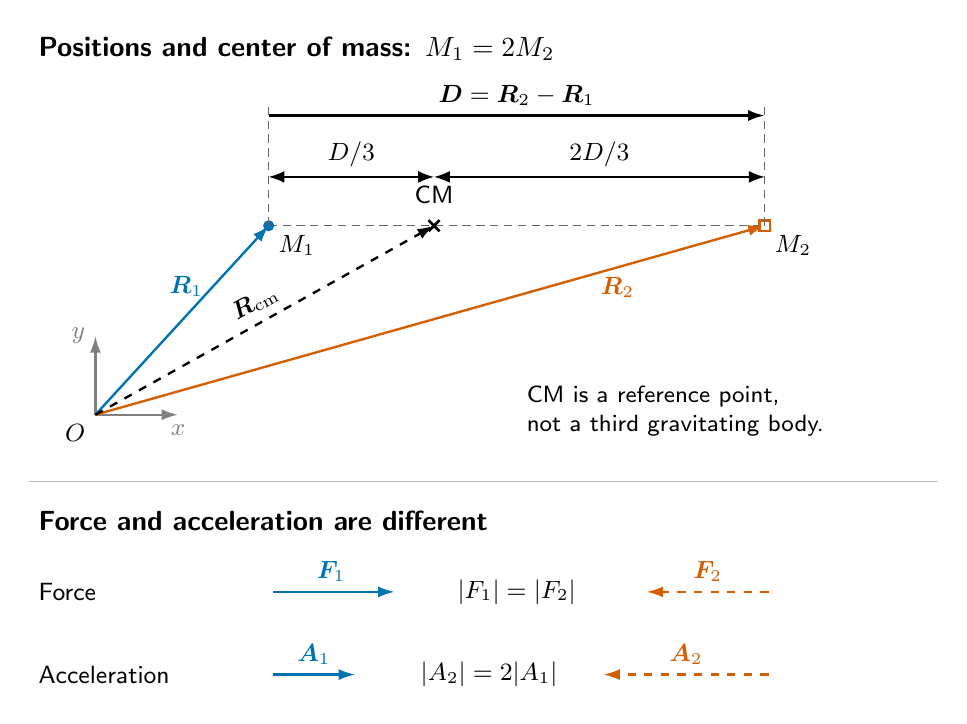
\begin{tikzpicture}[textbook diagram]
  \node[anchor=west,font=\sffamily\bfseries] at (0,4.75) {Positions and center of mass: $M_1=2M_2$};
  \coordinate (O) at (0.85,0.10);
  \coordinate (P) at (3.05,2.5);
  \coordinate (Q) at (9.35,2.5);
  \coordinate (C) at (5.15,2.5);
  \draw[vector,black!50] (O) -- +(1.05,0) node[below] {$x$};
  \draw[vector,black!50] (O) -- +(0,1.0) node[left] {$y$};
  \node[below left] at (O) {$O$};
  \draw[vector,figblue] (O) -- node[left,pos=0.68] {$\boldsymbol R_1$} (P);
  \draw[vector,figred] (O) -- node[below,pos=0.78] {$\boldsymbol R_2$} (Q);
  \draw[vector,black,dashed] (O) -- node[above,pos=0.50,sloped] {$\boldsymbol R_{\rm cm}$} (C);
  \draw[guide] (P) -- (Q);
  \fill[figblue] (P) circle (2.0pt);
  \draw[figred,line width=0.9pt,fill=white] ($(Q)+(-0.065,-0.065)$) rectangle ($(Q)+(0.065,0.065)$);
  \draw[black,line width=1pt] ($(C)+(-0.07,-0.07)$) -- ($(C)+(0.07,0.07)$);
  \draw[black,line width=1pt] ($(C)+(-0.07,0.07)$) -- ($(C)+(0.07,-0.07)$);
  \node[below right] at (P) {$M_1$};
  \node[below right] at (Q) {$M_2$};
  \node[above,yshift=1.5mm] at (C) {CM};
  \draw[vector] (3.05,3.90) -- node[above] {$\boldsymbol D=\boldsymbol R_2-\boldsymbol R_1$} (9.35,3.90);
  \draw[guide] (P) -- (3.05,4.02);
  \draw[guide] (Q) -- (9.35,4.02);
  \draw[<->] (3.05,3.12) -- node[above] {$D/3$} (5.15,3.12);
  \draw[<->] (5.15,3.12) -- node[above] {$2D/3$} (9.35,3.12);
  \node[hint,anchor=west] at (6.2,0.15) {CM is a reference point,\\not a third gravitating body.};
  \draw[black!25] (0,-0.75) -- (11.55,-0.75);
  \node[anchor=west,font=\sffamily\bfseries] at (0,-1.25) {Force and acceleration are different};
  \node[anchor=west] at (0,-2.15) {Force};
  \draw[vector,figblue] (3.1,-2.15) -- (4.65,-2.15) node[above,pos=0.48] {$\boldsymbol F_1$};
  \draw[vector,figred,dashed] (9.4,-2.15) -- (7.85,-2.15) node[above,pos=0.5] {$\boldsymbol F_2$};
  \node at (6.2,-2.15) {$|F_1|=|F_2|$};
  \node[anchor=west] at (0,-3.20) {Acceleration};
  \draw[vector,figblue] (3.1,-3.20) -- (4.15,-3.20) node[above,pos=0.5] {$\boldsymbol A_1$};
  \draw[vector,figred,dashed] (9.4,-3.20) -- (7.30,-3.20) node[above,pos=0.5] {$\boldsymbol A_2$};
  \node at (5.85,-3.20) {$|A_2|=2|A_1|$};
\end{tikzpicture}

\caption{質量比$M_1:M_2=2:1$の位置関係。任意の原点$O$と重心CMを区別しています。重心からの距離の比は$1:2$です。下段は力と加速度の違いで、力の大きさは等しくても加速度の大きさは異なります。段をまたいで矢印の長さを比較しません。}
\label{fig:concept-ch2-cm}
\end{figure}
\FloatBarrier
% END TikZ addition: ch02_center_of_mass

\begin{failbox}{単純な平均を重心にしない}
$(\Rvec_1+\Rvec_2)/2$が重心になるのは等質量のときだけです。同じく、$\Vvec_1=-\Vvec_2$と置けば重心が静止するとは限りません。位置にも速度にも、式\eqref{eq:ch2-inverse-transform}の質量比を使います。
\end{failbox}

\section{初期速度から軌道を選ぶ}
\label{sec:ch2-orbit-types}
\subsection{円軌道を基準にする}
相対距離が$D_0$の円軌道を考えます。相対運動の向心加速度と重力加速度を等しくすると、相対円運動速度と周期は
\begin{equation}
v_{\rm c}=\sqrt{\frac{\mu}{D_0}},\qquad
\Tc=2\pi\sqrt{\frac{D_0^3}{\mu}}
\label{eq:ch2-circle}
\end{equation}
です。ここでの$v_{\rm c}$は、一方の天体の速度ではなく、二つの\textbf{相対速度}の大きさです。重心系での各速度の大きさは、それぞれ$(M_2/\Mtot)v_{\rm c}$、$(M_1/\Mtot)v_{\rm c}$です。

初期位置と速度を
\begin{equation}
\Dvec(0)=(D_0,0),\qquad \Uvec(0)=(0,\eta v_{\rm c})
\label{eq:ch2-tangential-ic}
\end{equation}
と置きます。$\eta$は接線方向の初期速度を調整する無次元の数です。ここでは動径方向の初期速度は0で、$\eta>0$なら相対運動は反時計回りに始まります。

\subsection{比エネルギーで軌道を分類する}
相対運動の比エネルギーと比角運動量を
\begin{equation}
\varepsilon=\frac{U^2}{2}-\frac{\mu}{D},\qquad
\ell_z=D_xU_y-D_yU_x
\label{eq:ch2-specific-integrals}
\end{equation}
とします。どちらも式\eqref{eq:ch2-relative-ode}で保存されます。式\eqref{eq:ch2-tangential-ic}の初期値を代入すると、
\begin{equation}
\varepsilon_0=\frac{\mu}{D_0}\left(\frac{\eta^2}{2}-1\right),\qquad
\ell_{z,0}=\eta\sqrt{\mu D_0}
\label{eq:ch2-initial-integrals}
\end{equation}
です。初期速度を変えることは、同じ距離から始める軌道のエネルギーと角運動量を変えることに対応します。

点質量のKepler問題では、$\varepsilon<0$の非衝突軌道は楕円、$\varepsilon=0$は放物線、$\varepsilon>0$は双曲線です。円は楕円の特別な場合です。\cite{ryden2025} 本章の3例を表\ref{tab:ch2-types}にまとめます。
\begin{table}[htbp]
\centering\small
\caption{式\eqref{eq:ch2-tangential-ic}を使う3例。$D_0$と質量は共通で、変えるのは$\eta$だけです。}
\label{tab:ch2-types}
\begin{tabular}{llll}\toprule
$\eta$ & 軌道 & $\varepsilon_0$ & 初期位置の意味\\\midrule
$1$ & 円 & $-\mu/(2D_0)$ & 半径一定\\
$0.8$ & 楕円 & $-0.68\mu/D_0$ & 遠点\\
$\sqrt{2}$ & 放物線 & $0$ & 近点\\\bottomrule
\end{tabular}
\end{table}

$0<\eta<1$では初期速度が円運動速度より小さいため、距離は初期位置からいったん減少します。動径速度が0だった初期位置は遠点です。$\eta=\sqrt{2}$では脱出速度に相当し、初期位置から遠ざかって戻らない放物線になります。この例の放物線は、離れた場所から近づいてくる途中ではなく、\textbf{近点から出発する軌道}です。内向きに始める接近軌道は後で別に作ります。

\subsection{楕円の比較値を初期条件から求める}
数値結果を見る前に、楕円の大きさと周期を求めておきます。Kepler軌道の軌道長半径を$a_{\rm orb}$、離心率を$e$とすると、
\begin{equation}
a_{\rm orb}=-\frac{\mu}{2\varepsilon},\qquad
 e^2=1+\frac{2\varepsilon\ell_z^2}{\mu^2}
\label{eq:ch2-orbital-elements}
\end{equation}
です。\cite{ryden2025} 2次元なので、角運動量の大きさの2乗は$\ell_z^2$です。$0<\eta<1$の初期条件を代入すると、
\begin{equation}
a_{\rm orb}=\frac{D_0}{2-\eta^2},\qquad e=1-\eta^2,
\label{eq:ch2-ellipse-parameters}
\end{equation}
\begin{equation}
D_{\rm a}=D_0,\qquad D_{\rm p}=\frac{\eta^2D_0}{2-\eta^2},\qquad
T_{\rm ell}=2\pi\sqrt{\frac{a_{\rm orb}^3}{\mu}}.
\label{eq:ch2-ellipse-reference}
\end{equation}
添字aは遠点、pは近点です。$a_{\rm orb}$は相対軌道の長半径であり、後のPlummerモデルのスケール長ではありません。

\begin{notebox}{軌道の形と時間の関係}
楕円の形が分かっても、任意の時刻の位置を直ちに計算できるとは限りません。Kepler方程式を解いて時刻と軌道上の位置を対応させる方法もありますが、本章ではその求根算法を追加しません。円の同時刻の解析解と、楕円の解析周期後の戻り位置を、独立な位置の確認に使います。詳しい軌道の記述は文献\cite{ryden2025}に譲ります。
\end{notebox}

\section{Pythonで初期条件と重力を実装する}
\label{sec:ch2-implementation}
\subsection{単位・配列・標準条件をそろえる}
距離はkpc、時間はGyr、質量は$\Msun$とし、内部速度を$\mathrm{kpc\,Gyr^{-1}}$にそろえます。重力定数と速度の換算係数は第1章と同じです。以下では\texttt{import numpy as np}と\texttt{import matplotlib.pyplot as plt}を実行済みとします。

標準条件は本教材のために設定したもので、特定の実在天体の再現を目的としません。とくに、本章の天体は$10^{11}\Msun$程度の質量を持っていても、銀河の内部構造を持たない点質量です。
\inputcode{chap02/parameters}

\begin{table}[htbp]
\centering\small
\caption{本章の標準条件。3ケースとも同じ$\Tc$まで1000ステップで計算します。楕円の周期$T_{\rm ell}$とは区別します。数値は実行結果から生成しています。}
\label{tab:ch2-parameters}
\begin{tabular}{ll}\toprule
量 & 値\\\midrule
$M_1,M_2$ & $10^{11}\Msun,\ 5\times10^{10}\Msun$\\
$D_0$ & $20\unit{kpc}$\\
$v_{\rm c}$ & $\chtwovalVc\unit{km\,s^{-1}}$\\
$\Tc$ & $\chtwovalTc\unit{Gyr}$\\
$\Delta t=\Tc/1000$ & $\chtwovalDt\unit{Myr}$\\
$\eta$ & $1,\ 0.8,\ \sqrt{2}$\\
$\Rvec_{\rm cm}(0),\Vvec_{\rm cm}(0)$ & いずれも$\boldsymbol 0$\\\bottomrule
\end{tabular}
\end{table}

\texttt{masses[0]}が$M_1$、\texttt{masses[1]}が$M_2$です。位置配列\texttt{pos}と速度配列\texttt{vel}は形\texttt{(2, 2)}で、行が天体、列が$x,y$成分です。両者を横につないだ\texttt{state}は形\texttt{(2, 4)}で、各行に\texttt{[x, y, vx, vy]}を入れます。第1章の約束を変えず、天体の行を1行から2行へ増やしています。

\subsection{初期条件を関数にまとめる}
式\eqref{eq:ch2-inverse-transform}を関数にします。入力の\texttt{separation}は相対位置ベクトル、\texttt{relative\_\allowbreak velocity}は相対速度ベクトルです。どちらも2成分を渡します。重心位置・速度を省略したときは0とします。
\inputcode{chap02/initial-state}
\texttt{check\_masses}は、二つの質量が有限かつ正であることを確かめる短い補助関数です。実装はNotebookに含めています。検証のための分岐と、初期値を作る物理の式を区別して読んでください。

$D_0=20\unit{kpc}$、質量比$2:1$では、重心系の初期位置は$(-20/3,0)\unit{kpc}$と$(40/3,0)\unit{kpc}$です。二つの距離を足すと$20\unit{kpc}$になり、質量で重み付けした平均は0になります。

\subsection{同じ粒子対を使って加速度を返す}
最初に成分のまま計算し、向きと大きさを確認します。ここでは\texttt{state0}に上で作った初期値を入れたとします。
\inputcode{chap02/acceleration-scalar}
この初期位置で、天体1の$x$加速度は約$+562.31\unit{kpc\,Gyr^{-2}}$、天体2は約$-1124.62\unit{kpc\,Gyr^{-2}}$です。$y$成分はいずれも0です。重い天体1の加速度が小さくなっています。

次は、同じ計算を2成分のベクトルでまとめます。
\inputcode{chap02/acceleration-two-body}
\texttt{dr}が$\Dvec$、\texttt{np.dot(dr, dr)}が$D^2$です。返り値も形\texttt{(2, 2)}にそろえます。分母へ小さな数を足して特異点を隠しません。点質量モデルで距離が0なら、その条件はこのコードの対象外として停止します。

確認：\texttt{masses[0] * acc[0] + masses[1] * acc[1]}が、丸め誤差の範囲で0になっているか確かめてください。これは軌道を積分する前にできる確認です。

\section{KDKで両天体を同時に進める}
\label{sec:ch2-kdk}
\subsection{積分器ではなく加速度関数を替える}
時刻$t_n$における2天体の状態が分かっているとします。KDKを、それぞれの天体$k=1,2$に対して
\begin{align}
\Vvec_k^{n+1/2}&=\Vvec_k^n+\frac{\Delta t}{2}\boldsymbol A_k^n,\nonumber\\
\Rvec_k^{n+1}&=\Rvec_k^n+\Delta t\Vvec_k^{n+1/2},\nonumber\\
\boldsymbol A_k^{n+1}&=\boldsymbol A_k(\Rvec_1^{n+1},\Rvec_2^{n+1}),\nonumber\\
\Vvec_k^{n+1}&=\Vvec_k^{n+1/2}+\frac{\Delta t}{2}\boldsymbol A_k^{n+1}
\label{eq:ch2-kdk}
\end{align}
の順に行います。半整数ステップの速度は途中で使う値です。履歴には最後のkickを終えた、整数時刻の位置と速度を保存します。KDKの性質と導出は第1章で学んだ内容を使います。\cite{simten2007}

両天体の最初のkickを終えてから両天体をdriftし、その\textbf{新しい2位置をそろえて}次の加速度を計算します。配列全体を更新することで、この順序を簡単に保てます。
\inputcode{chap02/leapfrog-step}
第1章から変えたのは、最後の引数名を\texttt{mu}から\texttt{masses}へ替えた点です。今回は加速度関数に二つの質量を渡す必要があるためです。KDKの4行の計算と、加速度を返して再利用する構造は変わりません。

\begin{failbox}{片方だけを先に次の時刻へ進めない}
天体1の位置を更新してから、その新しい位置と天体2の古い位置を使って天体2を更新すると、式\eqref{eq:ch2-kdk}とは別の計算になります。同じ時刻に対する作用・反作用もそろいません。全天体のdriftを終えてから、次の加速度を一度に求めます。
\end{failbox}

\subsection{更新を繰り返して履歴を作る}
最初の加速度だけをループの前で求めます。その後は、前ステップで返された加速度を次の最初のkickに使います。
\inputcode{chap02/integrate-leapfrog}
\texttt{prepare\_history}は第1章と同じ役割の補助関数ですが、今回は初期状態の形\texttt{(2, 4)}を確認します。正のステップ数と最終時刻、有限の初期値を確認し、コピーと保存領域を用意します。履歴の形は\texttt{(n\_steps + 1, 2, 4)}です。

\texttt{history[n, 1, :2]}は時刻$t_n$における天体2の位置です。最初の軸が時間、次が天体、最後が位置・速度の成分であることを、確認してください。初期値も保存するので、出力時刻の数はステップ数より1つ多くなります。

本章でも、$N_{\rm step}$ステップのための加速度関数の呼び出しは$N_{\rm step}+1$回です。1回の呼び出しで\textbf{両方の加速度}を求めます。1000ステップなら1001回です。粒子対の計算が1組なので、高速化手法や並列化は必要ありません。

\subsection{3ケースを同じ条件で計算する}
各ケースの初期状態を作り直し、独立に積分します。一つの計算の最終状態を、次のケースの初期状態へ流用しないようにします。
\inputcode{chap02/run-cases}
本章の時間積分はすべてKDKです。RK4やEuler法との再比較は行いません。今回は積分法ではなく、初期条件、相対運動、保存量に注目します。

\section{重心系と相対座標で軌道を見る}
\label{sec:ch2-figures}
\subsection{2天体の軌道中心を確認する}
まず$\eta=0.8$の楕円の場合に、二つの軌道を別々に描きます。青実線と丸が天体1、朱色破線と四角が天体2、黒い星印が重心です。両天体の軌道を同じ軸に重ねると、重い天体が重心の近くを動いていることが分かります。
\inputcode{chap02/plot-barycentric}
\begin{figure}[htbp]
\centering\includegraphics[width=0.64\linewidth]{\figpath{ch02_barycentric}}
\caption{質量比$M_1:M_2=2:1$の楕円軌道を重心系で表示した結果。丸・四角は初期位置です。二つの軌道は重心を共通の焦点とし、大きさの比は$1:2$です。計算時間は$\Tc$で、楕円の約$\chtwovalEllPeriods$周期に相当します。}
\label{fig:ch2-barycentric}
\end{figure}

原点に星印があるからといって、そこに第3の質量を置いたわけではありません。力を及ぼしているのは、動いている2天体だけです。重心は、二つの質量から定義する位置です。

Notebookではこの履歴からアニメーションも作ります。画面の再生間隔を変えても、計算した軌道や物理的な時間は変わりません。本文の図も保存することで、動画なしでも軌道の違いを読めるようにします。

\subsection{相対軌道の形を比較する}
履歴の各時刻で天体2の位置から天体1の位置を引くと、相対軌道が得られます。式\eqref{eq:ch2-relative-ode}を満たす軌道として、円・楕円・放物線を比べられます。

本章の接線速度から始める初期条件では、相対位置の極角を$\phi$として、解析的な形を
\begin{equation}
D(\phi)=\frac{\eta^2D_0}{1+(\eta^2-1)\cos\phi}
\label{eq:ch2-conic}
\end{equation}
と書けます。これはKepler軌道の式へ初期条件を代入し、$\phi=0$を初期位置に選んだものです。\cite{ryden2025} $0<\eta<1$ではその位置が遠点なので、通常の「近点を角度0にする」式と分母の符号が異なって見えます。

\begin{figure}[htbp]
\centering\includegraphics[width=0.70\linewidth]{\figpath{ch02_relative_orbits}}
\caption{同じ$D_0$から、初期接線速度だけを変えた相対軌道。3ケースとも同じ$\Tc$まで計算しています。白抜き丸は式\eqref{eq:ch2-conic}による解析的な軌道形状上の点で、等時間間隔の点ではありません。星印は共通の初期相対位置です。}
\label{fig:ch2-relative}
\end{figure}

図\ref{fig:ch2-relative}の原点は相対座標での基準点です。この図だけでは、天体1が元の慣性系で静止しているようにも見えますが、実際の計算では図\ref{fig:ch2-barycentric}のように両天体が動いています。

また、解析的な曲線に数値解が重なっても、時刻と位置の対応まで正しいとは限りません。軌道の形の確認と、同じ時刻における位置の確認を分けて行います。

\section{2体系の保存量を確かめる}
\label{sec:ch2-conservation}
\subsection{全エネルギーと全角運動量を求める}
第1章では1粒子の比エネルギーを計算しました。今回は二つの質量を掛けた\textbf{全エネルギー}を計算します。2天体の運動エネルギーと、1組の粒子対のポテンシャルエネルギーは
\begin{equation}
K=\frac12M_1V_1^2+\frac12M_2V_2^2,\qquad
W=-\frac{GM_1M_2}{D},\qquad E=K+W
\label{eq:ch2-total-energy}
\end{equation}
です。距離$D$が変わると$K$と$W$はそれぞれ変わりますが、その和は一定です。例えば
\begin{equation}
\frac{dK}{dt}=-\frac{GM_1M_2}{D^3}\Dvec\cdot\Uvec,\qquad
\frac{dW}{dt}=+\frac{GM_1M_2}{D^3}\Dvec\cdot\Uvec
\label{eq:ch2-energy-balance}
\end{equation}
となり、変化率が打ち消し合います。\textbf{片方の天体のエネルギーだけを保存量としない}ことが、第1章との違いです。

固定した原点の周りの全角運動量の$z$成分は
\begin{equation}
L_z=\sum_{k=1}^{2}M_k(X_kV_{ky}-Y_kV_{kx})
\label{eq:ch2-total-angular}
\end{equation}
です。二つの内力は同じ直線上で逆向きに働くので、全トルクは0です。全角運動量も保存されます。全運動量$\Pvec$と重心の等速直線運動は、式\eqref{eq:ch2-momentum-conservation}、式\eqref{eq:ch2-cm-motion}で確かめます。

\begin{failbox}{ポテンシャルエネルギーを2回足さない}
粒子対のエネルギーは$-GM_1M_2/D$を1回だけ数えます。$M_1\Phi_2(\Rvec_1)+M_2\Phi_1(\Rvec_2)$をそのまま足すと、同じ相互作用を2回数えてしまいます。各天体で計算してから足す書き方では、全体に$1/2$が必要です。
\end{failbox}

\subsection{全エネルギーと相対運動の比エネルギーを区別する}
式\eqref{eq:ch2-specific-integrals}の$\varepsilon$と、式\eqref{eq:ch2-total-energy}の$E$は別の量です。この関係を整理するため、換算質量を
\begin{equation}
\mred=\frac{M_1M_2}{\Mtot}
\label{eq:ch2-reduced-mass}
\end{equation}
とします。式\eqref{eq:ch2-inverse-transform}を$K$へ代入すると、重心速度と相対速度の交差項が消え、
\begin{equation}
E=\frac12\Mtot V_{\rm cm}^2+\mred\varepsilon
\label{eq:ch2-energy-decomposition}
\end{equation}
です。同じように、
\begin{equation}
L_z=\Mtot(\Rvec_{\rm cm}\times\Vvec_{\rm cm})_z+\mred\ell_z
\label{eq:ch2-angular-decomposition}
\end{equation}
となります。重心系では、$E=\mred\varepsilon$、$L_z=\mred\ell_z$です。\cite{ryden2025}

$\mu=G\Mtot$は重力の強さを表すパラメータ、$\mred$は質量です。同じ記号で呼ばないようにします。$\varepsilon$の単位は$\mathrm{kpc^2\,Gyr^{-2}}$、$E$はそれに$\Msun$を掛けた単位です。また、束縛・非束縛の分類に使うのは\textbf{相対運動の}$\varepsilon$です。系全体を速く動かしたときの、任意の慣性系での$E$の符号ではありません。

\subsection{履歴から数値を求める}
位置と速度は、KDKの最後のkickまで終えた同じ時刻の値を使います。以下では履歴から各天体の量を取り出し、全エネルギー、全角運動量、全運動量、重心をまとめて返します。
\inputcode{chap02/diagnostics}
この関数は各保存量を保存するように補正するものではありません。得られた履歴を読み取り、値を計算するだけです。結果を見て毎ステップ重心や速度を修正すると、もとの積分器の誤差を評価できなくなります。

\subsection{初期値が0の量は相対誤差にしない}
重心系では$\Pvec(0)=\boldsymbol 0$です。放物線では、理論的に$E(0)=0$でもあります。これらを分母にした「相対誤差」は定義できません。浮動小数点計算で初期エネルギーが小さな非零値になっていても、それで割るのは不適切です。

そこで、本章では初期距離と相対円運動速度から、共通の正の基準量を作ります。
\begin{equation}
E_{\rm scale}=\frac{GM_1M_2}{D_0},\qquad
P_{\rm scale}=\Mtot v_{\rm c}.
\label{eq:ch2-error-scales}
\end{equation}
保存した全時刻にわたる最大値を使い、
\begin{align}
e_E&=\max_n\frac{|E^n-E^0|}{E_{\rm scale}},&
e_L&=\max_n\frac{|L_z^n-L_z^0|}{|L_z^0|},\nonumber\\
e_P&=\max_n\frac{|\Pvec^n-\Pvec^0|}{P_{\rm scale}},&
e_{\rm cm}&=\max_n\frac{|\Rvec_{\rm cm}^n-\Rvec_{\rm cm}^{\rm exact}(t_n)|}{D_0}
\label{eq:ch2-error-metrics}
\end{align}
とします。$\Rvec_{\rm cm}^{\rm exact}$は式\eqref{eq:ch2-cm-motion}です。本章の初期条件では$L_z^0\ne0$なので、角運動量にだけその初期値を使えます。動径軌道など$L_z^0=0$の問題では、角運動量にも別の基準量が必要です。
\inputcode{chap02/error-metrics}

\begin{table}[htbp]
\centering\small
\caption{3ケースの保存量・重心の確認。いずれも$\Tc$まで1000ステップのKDKです。エネルギーは$|E(0)|$ではなく、式\eqref{eq:ch2-error-scales}で規格化しています。}
\label{tab:ch2-conservation}
\begin{tabular}{lrrrr}\toprule
軌道 & $e_E$ & $e_L$ & $e_P$ & $e_{\rm cm}$ \\
\midrule
円 & $1.95\times 10^{-10}$ & $2.55\times 10^{-15}$ & $0$ & $0$ \\
楕円 & $5.72\times 10^{-5}$ & $5.42\times 10^{-15}$ & $0$ & $0$ \\
放物線 & $5.32\times 10^{-6}$ & $4.87\times 10^{-15}$ & $0$ & $0$ \\
\bottomrule\end{tabular}

\end{table}

表\ref{tab:ch2-conservation}は、配布コードの実行結果です。表示された0は、この質量比と対称な初期配置をこの実装で計算したとき、対応する引き算が浮動小数点演算でも0になったことを意味します。任意の質量比・初期値で誤差が必ず0になる、という主張ではありません。後で重心を動かした場合も確認します。

\begin{figure}[htbp]
\centering\includegraphics[width=0.76\linewidth]{\figpath{ch02_energy}}
\caption{エネルギー差の時間変化。変化の向きも分かるよう、絶対値を取らない$[E(t)-E(0)]/E_{\rm scale}$を描いています。楕円で差が大きくなる時期は、近点付近に対応します。}
\label{fig:ch2-energy}
\end{figure}

\subsection{保存量ごとに誤差が異なる理由を考える}
KDKでは、同じ位置から求めた二つの力が打ち消し合うため、kickは全運動量を保ちます。driftは速度を変えません。全角運動量についても、kickでの全トルクが0で、driftの追加項は$\Vvec_k\times\Vvec_k=0$です。このため、本章の中心力の粒子対を正しく計算すれば、全運動量と全角運動量のずれは丸め誤差程度になります。

一方、KDKは全エネルギーを毎ステップ厳密に保存する方法ではありません。図\ref{fig:ch2-energy}のように、有限の刻みによる差が現れます。全運動量と全角運動量がよく保存されていても、エネルギーや軌道の位相まで同じ精度で正しいとは限りません。

\section{軌道の時間変化と刻みを確認する}
\label{sec:ch2-accuracy}
\subsection{近点と遠点を測る}
式\eqref{eq:ch2-ellipse-parameters}と式\eqref{eq:ch2-ellipse-reference}によれば、$\eta=0.8$の標準例は$e=0.36$、$a_{\rm orb}=\chtwovalEllA\unit{kpc}$、$D_{\rm p}=\chtwovalEllRp\unit{kpc}$です。周期は$T_{\rm ell}=\chtwovalEllP\unit{Gyr}$で、基準の円軌道周期$\Tc$より短くなります。

図\ref{fig:ch2-separation}の円軌道では、距離はほぼ一定です。楕円では近点と遠点の間を往復し、放物線では近点から遠ざかります。楕円は$\Tc$の間に1周以上するので、距離の谷が複数現れます。
\begin{figure}[htbp]
\centering\includegraphics[width=0.76\linewidth]{\figpath{ch02_separation}}
\caption{2天体間距離の時間変化。横軸の$\Tc$は3ケース共通の基準時間で、楕円の周期ではありません。点線は楕円の場合の解析的な近点距離です。}
\label{fig:ch2-separation}
\end{figure}

標準計算で保存された楕円の最小距離は$\chtwovalEllMin\unit{kpc}$でした。解析値との差には、時間積分の誤差に加えて、\textbf{真の近点通過時刻と保存時刻が一致しない}影響も含まれます。\texttt{np.argmin}で得るのは、保存された配列の最小要素です。連続時間の最小値そのものを解いているわけではありません。

\subsection{保存量とは別に位置を比較する}
円軌道には、第1章と同じ形の時刻に依存する解析解があります。
\begin{equation}
\Dvec_{\rm circ}^{\rm exact}(t)=D_0\left(\cos\Omega t,\sin\Omega t\right),\qquad
\Omega=\sqrt{\frac{\mu}{D_0^3}}.
\label{eq:ch2-exact-circle}
\end{equation}
同じ時刻における数値相対位置との差を取り、
\begin{equation}
e_{\rm circ}=\max_n\frac{|\Dvec^n-\Dvec_{\rm circ}^{\rm exact}(t_n)|}{D_0}
\label{eq:ch2-circle-error}
\end{equation}
を測ります。半径の差ではなく位置ベクトルの差なので、位相のずれも検出します。
\inputcode{chap02/exact-circle}

楕円では任意時刻の位置を解く代わりに、\textbf{解析的に求めた周期}$T_{\rm ell}$を使います。ちょうど1周期後には初期位置へ戻るはずなので、
\begin{equation}
e_{\rm ret}=\frac{|\Dvec^{N_{\rm step}}-\Dvec(0)|}{D_0},\qquad
 t_{N_{\rm step}}=T_{\rm ell}
\label{eq:ch2-return-error}
\end{equation}
を確認します。これは1周期後の戻り位置の誤差であり、途中も含めた最大誤差ではありません。数値解が戻った時刻を探してから、そこを周期と呼ぶ方法ではない点が重要です。

\subsection{同じ最終時刻で刻みを細かくする}
円軌道は$\Tc$まで、楕円は$T_{\rm ell}$まで計算し、それぞれの系列の中でステップ数だけを変えます。二つの系列の最終時刻は異なりますが、同じ系列では固定されています。二つの誤差の定義も異なるため、値の大小をそのまま「円と楕円の難しさ」の尺度にはしません。
\inputcode{chap02/convergence}

\begin{table}[htbp]
\centering\small
\caption{KDKの時間刻み試験。円は解析的な1周期までの最大位置誤差、楕円は解析的な1周期後の戻り位置の誤差を示します。$p$は一つ前の行との誤差比から求めた推定次数です。}
\label{tab:ch2-convergence}
\begin{tabular}{rrrrr}\toprule
$N_{\rm step}$ & $e_{\rm circ}$ & $p$ & $e_{\rm ret}$ & $p$ \\
\midrule
100 & $8.63\times 10^{-3}$ & --- & $9.13\times 10^{-3}$ & --- \\
200 & $2.16\times 10^{-3}$ & 1.9985 & $2.29\times 10^{-3}$ & 1.9927 \\
400 & $5.40\times 10^{-4}$ & 1.9996 & $5.74\times 10^{-4}$ & 1.9982 \\
800 & $1.35\times 10^{-4}$ & 1.9999 & $1.44\times 10^{-4}$ & 1.9995 \\
\bottomrule\end{tabular}

\end{table}

刻みを半分にしたときの誤差比から、
\begin{equation}
p=\frac{\log[e(\Delta t)/e(\Delta t/2)]}{\log 2}
\label{eq:ch2-order}
\end{equation}
を求めます。表\ref{tab:ch2-convergence}の最も細かい刻み側では、円が$\chtwovalOrderC$、楕円が$\chtwovalOrderEll$で、2へ近づいています。第1章の1粒子の場合から2体へ変えても、KDKの2次精度を確認できます。
\begin{figure}[htbp]
\centering\includegraphics[width=0.76\linewidth]{\figpath{ch02_convergence}}
\caption{時間刻みと位置誤差の両対数表示。横軸は各系列の積分区間に対する刻みの比で、どちらも$1/N_{\rm step}$です。点線は円の最も細かい刻みの点を通る傾き2の参照線です。数値データへの当てはめではありません。}
\label{fig:ch2-convergence}
\end{figure}

近点付近では距離が小さくなり、速度と加速度が大きく変わります。同じ刻みでも、円軌道より厳しい条件になることがあります。離心率をさらに大きくするときや、近点距離を小さくするときには、その新しい条件で刻み試験を行います。標準条件で得た誤差を、そのまま別の軌道の誤差とはみなしません。

\begin{notebox}{近点通過時刻の決め方}
保存された距離の最小値を使う以外に、距離を時間の関数として補間したり、動径速度$\Dvec\cdot\Uvec/D$が0になる時刻を探したりする方法もあります。本章では新しい補間法・求根法を追加せず、最小値が保存時刻に依存することを明示します。補間と求根の基本は、第3・4章で別の具体例から学びます。
\end{notebox}

\clearpage
\section{近点距離を指定して接近させる}
\label{sec:ch2-encounter}
\subsection{遠くから内向きに始める}
これまでの放物線は、動径速度0の近点から始めました。銀河相互作用の準備では、離れた位置から互いに近づく初期条件が便利です。ここでは初期距離$D_0$と目標近点距離$D_{\rm p}$を指定し、$0<D_{\rm p}<D_0$とします。

放物線では$\varepsilon=0$です。近点では速度は接線方向だけなので、式\eqref{eq:ch2-specific-integrals}から
\begin{equation}
U_{\rm p}^2=\frac{2\mu}{D_{\rm p}},\qquad
\ell_z=D_{\rm p}U_{\rm p}=\sqrt{2\mu D_{\rm p}}
\label{eq:ch2-pericenter-angular}
\end{equation}
です。角運動量保存より、初期距離での接線速度は$U_t=\ell_z/D_0$です。初期位置でもエネルギー0とし、内向きの符号を選ぶと、
\begin{equation}
U_t=\frac{\sqrt{2\mu D_{\rm p}}}{D_0},\qquad
U_r=-\sqrt{\frac{2\mu}{D_0}-U_t^2}
\label{eq:ch2-incoming-velocity}
\end{equation}
になります。初期位置を$\Dvec=(D_0,0)$とすれば、$\Uvec=(U_r,U_t)$をそのまま渡せます。ここでも原点を重心にした各天体の初期値へ、式\eqref{eq:ch2-inverse-transform}で変換します。
\inputcode{chap02/parabolic-encounter}

\subsection{指定した近点の再現性を確かめる}
この追加実験では、質量は標準例のまま、$D_0=60\unit{kpc}$、$D_{\rm p}=8\unit{kpc}$、最終時刻$0.60\unit{Gyr}$、1200ステップとします。刻みは$0.5\unit{Myr}$です。3ケース比較の$D_0$や$\Tc$と混同しないよう、条件を分けて記録します。

得られる初期相対速度は、$U_r=\chtwovalEncVr\unit{km\,s^{-1}}$、$U_t=\chtwovalEncVt\unit{km\,s^{-1}}$です。内向きの動径速度が負であることを確認してください。計算後に保存された最小距離は$\chtwovalEncMin\unit{kpc}$、その保存時刻は$\chtwovalEncTime\unit{Gyr}$でした。指定した$8\unit{kpc}$へ近づき、その後は離れていきます。
\begin{figure}[htbp]
\centering\includegraphics[width=0.76\linewidth]{\figpath{ch02_incoming_encounter}}
\caption{点質量2体の内向きに始まる放物線遭遇。破線は指定した近点距離、四角は保存された距離の最小値です。これは本章の質量比$2:1$の計算であり、後の等質量Plummer銀河の標準実験とは別の条件です。}
\label{fig:ch2-encounter}
\end{figure}

近づいた後に離れていくことは、計算の失敗ではありません。摩擦のない点質量2体では相対エネルギーが保存されるため、放物線遭遇が自動的に束縛軌道へ変わることはありません。近接通過と合体は区別します。

本章の式\eqref{eq:ch2-incoming-velocity}は、ポテンシャルが$-\mu/D$の場合の式です。第5章で有限サイズを表す中心間重力へ替えたとき、$\mu$だけを同じにしてこの速度を使えば、同じ近点距離が得られるとは限りません。\textbf{重力のモデルを変更したら、そのモデルに対応するエネルギーと初期条件を使う}という原則を引き継ぎます。

\section{条件を一つずつ変えて確かめる}
\label{sec:ch2-experiments}
\subsection{重心を等速で動かす}
計算の原点や、系全体の等速運動を変えても、相対運動は変わらないはずです。式\eqref{eq:ch2-inverse-transform}の重心位置を$(5,-3)\unit{kpc}$、重心速度を$(30,-20)\unit{km\,s^{-1}}$として、同じ楕円を計算します。
\inputcode{chap02/boost-experiment}
相対軌道の差を$D_0$で割った最大値は$\chtwovalBoostRel$、重心が式\eqref{eq:ch2-cm-motion}の直線から外れる量は$D_0$単位で$\chtwovalBoostCm$でした。これらは本実装での丸め誤差程度の差です。重心系の計算でたまたま誤差が0になった場合だけでなく、移動する重心でも確認する意味があります。

このとき、任意の原点の周りの$E$や$L_z$の初期値は、重心系と同じとは限りません。比較すべきなのは、それぞれの系で保存する量と、式\eqref{eq:ch2-energy-decomposition}・式\eqref{eq:ch2-angular-decomposition}の関係です。

\subsection{全質量を固定して質量比を変える}
次は$\Mtot,D_0,\Uvec(0)$を固定し、$q=M_2/M_1$だけを変えます。相対運動の式に現れるのは$\mu=G\Mtot$なので、相対軌道は同じです。しかし、各天体が重心から離れる距離は変わります。
\begin{table}[htbp]
\centering\small
\caption{全質量を固定した質量比の比較。相対軌道の差は、標準の$q=0.5$との差の最大値です。初期相対速度は$0.8v_{\rm c}$に固定しています。}
\label{tab:ch2-mass-ratio}
\begin{tabular}{rrrr}\toprule
$q=M_2/M_1$ & $|\Rvec_1(0)|\ [\mathrm{kpc}]$ & $|\Rvec_2(0)|\ [\mathrm{kpc}]$ & 相対軌道の差$/D_0$ \\
\midrule
1.0 & 10.000000 & 10.000000 & $1.57\times 10^{-14}$ \\
0.5 & 6.666667 & 13.333333 & $0$ \\
0.1 & 1.818182 & 18.181818 & $4.04\times 10^{-14}$ \\
\bottomrule\end{tabular}

\end{table}

$M_1$を固定したまま$M_2$を変えると、$\Mtot$も変わるので別の実験です。パラメータを変えたときには、何を固定し、何が連動して変わるかを記録します。これは銀河相互作用の比較実験にも必要な習慣です。

\section{本章のまとめ}
\label{sec:ch2-summary}
本章では、互いに重力を及ぼす2天体をKDKで動かしました。第1章から積分法を作り直すのではなく、2天体の同じ時刻の位置から加速度を返す関数へ替えました。最後に評価した加速度を再利用し、両天体の位置と速度を整数時刻にそろえて保存しました。

重心は全質量による重み付き平均です。相対運動には$\mu=G(M_1+M_2)$が入り、各天体の軌道は重心運動と相対運動から作られます。初期接線速度を変えると、円・楕円・放物線を作れることも確認しました。

保存量は、今回は2体系の全エネルギー・全角運動量・全運動量です。放物線のように初期エネルギーが0の問題では、その値で誤差を割りません。保存量だけでなく、円の同時刻の位置、楕円の1周期後の戻り位置、刻みを変えた収束も確かめました。

最後に、初期距離と近点距離から内向きの接近軌道を作りました。ただし、本章の重力源はまだ点質量です。第3章では、質量に広がりをもつ球対称のPlummerモデルを導入し、その中の星の運動へ進みます。点質量の式と広がった銀河の式を、混同しないことが重要です。

\chapterexercises
\paragraph{演習2.1　確認：重心と作用・反作用}
$M_1=10^{11}\Msun$、$M_2=5\times10^{10}\Msun$、$D_0=20\unit{kpc}$の円軌道を重心系に置いてください。初期位置と各天体の速度を求め、全運動量が0になることを示してください。また、初期加速度の大きさの比と、力の大きさの比を求めてください。

\paragraph{演習2.2　確認：楕円の形と周期}
同じ$D_0$で$\eta=0.8$としたとき、初期位置が遠点である理由を説明してください。$e,a_{\rm orb},D_{\rm p},T_{\rm ell}$を初期条件から求め、数値計算の距離の時間変化と比較してください。保存された最小距離と解析的な近点距離が完全には一致しない理由も述べてください。

\paragraph{演習2.3　確認：放物線のエネルギー誤差}
$\eta=\sqrt{2}$の計算で、$|E(t)-E(0)|/|E(0)|$を誤差に使わない理由を説明してください。本章の$E_{\rm scale}$で規格化すると、どの物理的な大きさに対するずれを測ることになるでしょうか。

\paragraph{演習2.4　応用：全質量を固定する}
表\ref{tab:ch2-mass-ratio}と同じ条件で$q=1,0.5,0.1$を比較してください。各天体の重心からの距離が変わっても、相対軌道が同じになることを確認してください。$M_1$だけを固定して$q$を変えた場合と、何が異なるか説明してください。

\paragraph{演習2.5　応用：移動する重心}
重心に位置$(5,-3)\unit{kpc}$、速度$(30,-20)\unit{km\,s^{-1}}$を与えてください。重心が等速直線運動し、相対軌道がもとの楕円と同じになるか確かめてください。任意の慣性系での全エネルギー$E$の符号だけでは、束縛軌道かどうかを判断できない理由も説明してください。

\paragraph{演習2.6　応用：KDKの時間反転}
標準の楕円を$\Tc$まで計算し、その最終位置を保ったまま、\textbf{両天体の速度}を符号反転してください。同じ正の時間刻みでさらに$\Tc$だけ進めたとき、初期位置と初期速度の符号反転へ戻るか確認してください。時間反転の試験に通ることだけで、軌道の位相誤差が小さいと言えるでしょうか。

\paragraph{演習2.7　発展：脱出速度を超える軌道}
$\eta=1.6$として、ほかは3ケース比較と同じ条件で計算してください。相対エネルギーの符号と離心率を求め、軌道が双曲線になることを確認してください。$\Tc$後の距離を放物線の場合と比べ、全エネルギーの誤差も確認してください。積分器の変更は必要ありません。

\newcommand{\chthreevalRhoZero}{8.8419\times 10^{8}}
\newcommand{\chthreevalVc}{226.475925}
\newcommand{\chthreevalVcInt}{231.619684}
\newcommand{\chthreevalTc}{0.162763}
\newcommand{\chthreevalTend}{0.813815}
\newcommand{\chthreevalDt}{0.162763}
\newcommand{\chthreevalMassError}{3.67\times 10^{-5}}
\newcommand{\chthreevalMassOrder}{2.0004}
\newcommand{\chthreevalRh}{3.914303805}
\newcommand{\chthreevalRhExact}{3.914298080}
\newcommand{\chthreevalRhError}{5.73\times 10^{-6}}
\newcommand{\chthreevalRootResidual}{3.93\times 10^{-10}}
\newcommand{\chthreevalTrueResidual}{8.12\times 10^{-7}}
\newcommand{\chthreevalRootWidth}{6.98\times 10^{-9}}
\newcommand{\chthreevalRootHalvings}{30}
\newcommand{\chthreevalRootCalls}{31}
\newcommand{\chthreevalOrbitOrder}{2.00005}
\newcommand{\chthreevalPeri}{3.027147967}
\newcommand{\chthreevalPeriSaved}{3.027207825}
\newcommand{\chthreevalCircEnergy}{1.62\times 10^{-10}}
\newcommand{\chthreevalNoncEnergy}{1.83\times 10^{-5}}
\newcommand{\chthreevalRootFloor}{9.16\times 10^{-5}}
\newcommand{\chthreevalNoncRatio}{3.99992}
\newcommand{\chthreevalAccelX}{-8.9413\times 10^{3}}
\newcommand{\chthreevalOutsideFractions}{0.057134,0.014815,0.003738}
\newcommand{\chthreevalScaleVcSeries}{255.834,226.476,159.196}
\newcommand{\chthreevalScaleRhSeries}{1.957149,3.914298,7.828596}

\chapter{銀河の中で星を動かす}
\label{chap:plummer}

第2章では、二つの天体を点質量として動かしました。ここからは、銀河の内部へ目を向けます。銀河の質量は中心の1点だけに集まっているわけではありません。中心からの距離によって、内側に含まれる質量も、星が受ける重力も変わります。本章では、その広がりを球対称のPlummerモデルで表します。

新しく学ぶ数値計算法は、\textbf{台形則}と\textbf{二分法}です。密度を積分して質量分布を求め、その質量の半分を含む半径を探します。さらに、第1・2章で使ったKDK leapfrogで、銀河の重力場中の星を動かします。数値積分、求根、時間積分を、一つの銀河モデルの中で区別して使うことが目標です。

\begin{goalbox}[この章で学ぶこと]
\begin{itemize}
\item 球対称の密度、内側の質量、ポテンシャル、重力加速度の関係を説明できます。
\item 台形則を実装し、Plummer球の質量分布を解析式と比較できます。
\item 二分法で半質量半径を求め、求根の残差と半径の誤差を区別できます。
\item Plummerポテンシャルに対応する円運動速度を与え、KDKで円軌道と非円軌道を計算できます。
\item 積分範囲、空間の分割、求根の許容幅、時間刻みが、それぞれ何に影響するかを確認できます。
\end{itemize}
\end{goalbox}

\section{質点のモデルを広がった銀河へ拡張する}
\label{sec:ch3-model}
\subsection{星を表す1粒子を動かす}
原点に中心を持つ、静的で球対称な銀河を考えます。その中を動く星を1個のテスト粒子で表します。粒子は銀河の重力を受けますが、銀河の密度やポテンシャルを変えません。銀河自身の粒子を多数用意して、その自己重力を計算するわけではありません。

第2章のように二つの有限質量が互いに動く問題とは違い、今回は重力場を固定します。これは銀河相互作用を始める前に、1個の銀河の重力を理解するための段階です。銀河中心が動く場合は第5章で扱います。

粒子の位置を$\rvec=(x,y)$、速度を$\vvec=(v_x,v_y)$とし、$r=|\rvec|$を原点からの距離とします。銀河は3次元の球ですが、初期位置と初期速度を$x$--$y$平面内に選べば、中心力による運動はその平面内にとどまります。\textbf{2次元で軌道を描くことと、2次元の質量分布を仮定することは別です。}\nobreak\cite{bt2008}

\subsection{球の大きさと計算する範囲を区別する}
本章では、球全体の質量を$M$、その広がりを表すスケール長を$a$とします。$a$は第2章で使ったKepler楕円の軌道長半径$a_{\rm orb}$ではありません。また、加速度ベクトル$\avec$とも区別します。

Plummerモデルの密度は、有限の半径で突然0にはなりません。外側ほど小さくなり、無限遠まで続きますが、全質量は有限です。後で使う$r_{\rm tab}$は、質量の表を作る範囲の上限です。$r=r_{\rm tab}$で密度や重力を切断するという意味ではありません。

\section{密度から質量と重力を求める}
\label{sec:ch3-spherical}
\subsection{薄い球殻に含まれる質量を求める}
球対称なら、密度$\rho(r)$は半径だけの関数です。半径$r$から$r+dr$までの薄い球殻の体積は$4\pi r^2dr$ですから、その質量は
\begin{equation}
 dM=4\pi r^2\rho(r)\,dr
 \label{eq:ch3-shell}
\end{equation}
です。中心から半径$r$まで足し合わせると、内側の質量は
\begin{equation}
 M(<r)=4\pi\int_0^r r'^2\rho(r')\,dr'
 \label{eq:ch3-enclosed-general}
\end{equation}
となります。$r'$は積分の途中で使う半径です。$M(<r)$は$r$に依存する量、$M$は球全体の一定の質量として使い分けます。


% BEGIN TikZ addition: ch03_spherical_shell
図\ref{fig:concept-ch3-shell}では、薄い球殻とその内側を分けて示しています。図は断面ですが、積分する質量には3次元の球殻の体積を使います。
\begin{figure}[!htbp]
\centering
% A cross-section of a three-dimensional shell, not a material outer boundary.
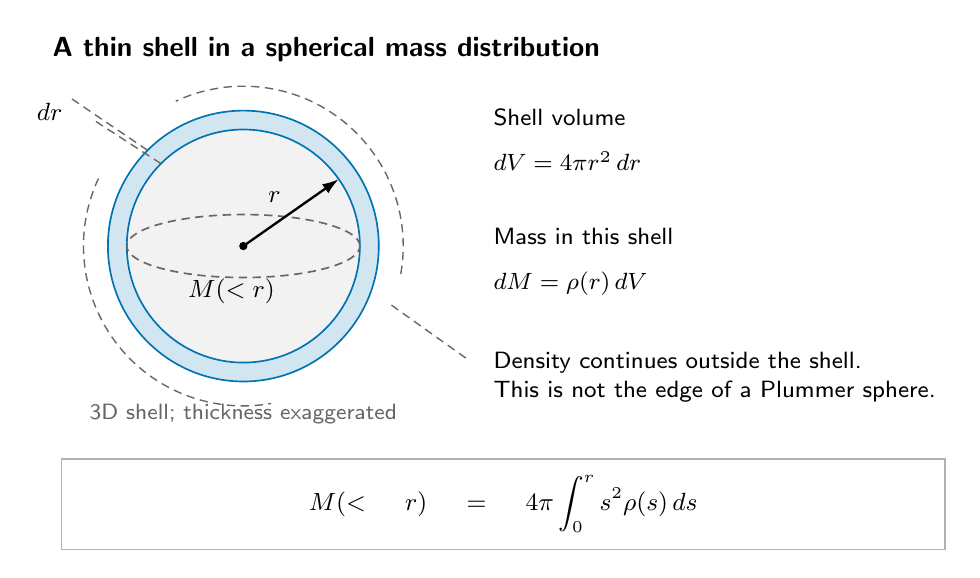
\begin{tikzpicture}[textbook diagram]
  \node[anchor=west,font=\sffamily\bfseries] at (0,4.85) {A thin shell in a spherical mass distribution};
  \coordinate (O) at (2.55,2.35);
  \path[fill=black!5] (O) circle (1.48);
  \path[fill=figblue!18,even odd rule] (O) circle (1.72) (O) circle (1.48);
  \draw[figblue] (O) circle (1.48);
  \draw[figblue] (O) circle (1.72);
  \draw[guide] ($(O)+(-10:2.03)$) arc[start angle=-10,end angle=115,radius=2.03];
  \draw[guide] ($(O)+(155:2.03)$) arc[start angle=155,end angle=280,radius=2.03];
  \draw[figgray,densely dashed] (O) ellipse (1.48 and 0.40);
  \fill (O) circle (1.5pt);
  \draw[vector] (O) -- ($(O)+(35:1.48)$) node[midway,above left] {$r$};
  \draw[guide] ($(O)+(135:1.48)$) -- (0.65,3.95);
  \draw[guide] ($(O)+(135:1.72)$) -- (0.37,4.22);
  \node[anchor=east] at (0.38,4.05) {$dr$};
  \node at (2.4,1.78) {$M(<r)$};
  \node[small label,text=figgray] at (2.55,0.22) {3D shell; thickness exaggerated};
  \node[hint,anchor=west,text width=57mm] at (5.6,3.70) {Shell volume\\[2mm]$dV=4\pi r^2\,dr$};
  \node[hint,anchor=west,text width=57mm] at (5.6,2.15) {Mass in this shell\\[2mm]$dM=\rho(r)\,dV$};
  \node[hint,anchor=west,text width=57mm] at (5.6,0.68) {Density continues outside the shell.\\This is not the edge of a Plummer sphere.};
  \draw[guide] (4.43,1.60) -- (5.4,0.91);
  \node[draw=black!30,fill=white,text width=108mm,align=center,inner sep=6pt] at (5.85,-0.93) {$\displaystyle M(<r)=4\pi\int_0^r s^2\rho(s)\,ds$};
\end{tikzpicture}

\caption{3次元の球殻を断面で示した図。色の付いた殻の厚さ$dr$を強調しており、殻の体積は$4\pi r^2dr$です。内側の薄灰色の領域が$M(<r)$に対応します。殻の外にも密度は続き、この円をPlummer球の外縁とはみなしません。}
\label{fig:concept-ch3-shell}
\end{figure}
\FloatBarrier
% END TikZ addition: ch03_spherical_shell

\begin{failbox}{軌道が平面内でも、球殻の体積は変わりません}
式\eqref{eq:ch3-shell}に必要なのは$4\pi r^2$です。図が2次元だからといって$2\pi r$へ替えません。後者は、面密度から円環内の質量を求める場合の因子です。第4章の円盤では、体積密度$\rho$とは異なる面密度$\Sigma$を使います。
\end{failbox}

\subsection{内側の質量から重力加速度を求める}
球対称な殻が内部へ及ぼす重力は、各方向からの寄与が打ち消し合います。一方、殻の外では、その質量を中心へ集めた場合と同じ重力になります。Newtonの球殻に関する定理を使うと、半径$r>0$での加速度は、内側の質量だけで決まります。\cite{bt2008}
\begin{equation}
 \avec(\rvec)=-\frac{G M(<r)}{r^3}\rvec.
 \label{eq:ch3-enclosed-force}
\end{equation}
向きは中心向き、大きさは$GM(<r)/r^2$です。点質量の場合と似ていますが、ここでは分子の$M(<r)$が半径に応じて変わります。

円運動をする星では、重力加速度と向心加速度が等しくなります。円運動速度$v_c$は
\begin{equation}
 \frac{v_c^2(r)}{r}=\frac{G M(<r)}{r^2},
 \qquad v_c^2(r)=\frac{G M(<r)}{r}=r\frac{d\Phi}{dr}
 \label{eq:ch3-vc-general}
\end{equation}
です。$\Phi$は単位質量当たりの重力ポテンシャルで、$\avec=-\nabla\Phi$と定義します。

\begin{notebox}{内側の質量だけでポテンシャルも書けるでしょうか}
一般の球対称分布では、$\Phi(r)=-GM(<r)/r$とは書けません。外側の殻は、内部の力には寄与しなくても、ポテンシャルには寄与するためです。$\Phi(\infty)=0$と選ぶと、$r>0$について
\[
 \Phi(r)=-G\left[\frac{M(<r)}{r}+4\pi\int_r^\infty r'\rho(r')\,dr'\right]
\]
です。詳しい導出は文献\cite{bt2008}の\S2.2.1に譲ります。本章では、次に示すPlummerポテンシャルの解析式を使います。
\end{notebox}

\section{Plummerモデルを導入する}
\label{sec:ch3-plummer}
\subsection{密度とポテンシャルを対応させる}
中心で有限の密度を持ち、外側で滑らかに薄くなる簡単なモデルとして、Plummer球を選びます。密度とポテンシャルは
\begin{align}
 \rho(r)&=\frac{3M}{4\pi a^3}\left(1+\frac{r^2}{a^2}\right)^{-5/2},
 \label{eq:ch3-density}\\
 \Phi(r)&=-\frac{GM}{\sqrt{r^2+a^2}}
 \label{eq:ch3-potential}
\end{align}
です。これらは同じ質量分布を表す一組の式です。文献\cite{bt2008}のPlummerスケール長$b$を、本書では$a$と書きます。どちらかの式だけで$a$を変更すると、異なるモデルを混ぜてしまいます。

中心密度は$\rho(0)=3M/(4\pi a^3)$です。全質量を固定して$a$を大きくすると、中心密度が下がり、質量が広く分布します。外側では$\rho\propto r^{-5}$となり、$\Phi$は点質量の$-GM/r$へ近づきます。$a$は銀河の外縁ではなく、中心側と外側の振る舞いが変わる長さの尺度です。

\subsection{内側の質量を解析的に求める}
数値積分を始める前に、比較に使う解析式を求めます。式\eqref{eq:ch3-density}を式\eqref{eq:ch3-enclosed-general}へ代入すると、
\begin{equation}
 M(<r)=3Ma^2\int_0^r \frac{r'^2}{(r'^2+a^2)^{5/2}}\,dr'
 \label{eq:ch3-mass-integral}
\end{equation}
です。ここで
\begin{equation}
 \frac{d}{dr'}\left[\frac{r'^3}{(r'^2+a^2)^{3/2}}\right]
 =\frac{3a^2r'^2}{(r'^2+a^2)^{5/2}}
 \label{eq:ch3-mass-derivative}
\end{equation}
を使うと、積分の結果は
\begin{equation}
 \boxed{M(<r)=M\frac{r^3}{(r^2+a^2)^{3/2}}}
 \label{eq:ch3-mass-exact}
\end{equation}
になります。この式は、採用した密度から本章で直接計算したものです。$r=0$で0、$r\to\infty$で$M$になり、$r>0$では単調に増えます。$r=a$では$M(<a)/M=2^{-3/2}\simeq0.3536$なので、$a$は半質量半径でもありません。

\subsection{単位と標準パラメータを決める}
前章と同じく、内部単位はkpc、Gyr、$\Msun$です。速度は内部では$\mathrm{kpc\,Gyr^{-1}}$を使い、図や数値の表示でだけ$\mathrm{km\,s^{-1}}$へ換算します。以下ではNumPyを\texttt{np}、Matplotlibの\texttt{pyplot}を\texttt{plt}として読み込んでいるものとします。

\inputcode{chap03/parameters}

本章の$M=10^{11}\Msun$、$a=3\unit{kpc}$は教材用の設定です。特定の実在銀河を再現する値ではありません。$r_{\rm tab}=5a=15\unit{kpc}$までの質量表を、標準では256区間、257分点で作ります。\texttt{root\_xtol}の役割は、二分法の節で説明します。

密度、ポテンシャル、解析的な質量を、それぞれ短い関数にします。\texttt{radius}には1個の半径も、半径を並べた配列も渡せます。
\inputcode{chap03/plummer-model}
ここで半径の配列を使うのは、\textbf{同じ銀河の半径方向の表}を作るためです。複数の星の運動を同時に計算しているわけではありません。

\Needspace{10\baselineskip}
\section{台形則で内側の質量を求める}
\label{sec:ch3-trapezoid}
\subsection{積分する関数を決める}
式\eqref{eq:ch3-mass-exact}を使えば質量はすぐ求まります。それでも数値積分を行うのは、正解の分かる問題で算法と実装を確かめるためです。解析的に積分できない密度や、分点上の値だけが与えられる場合にも、同じ考え方を使えます。

積分する関数を
\begin{equation}
 g(r)=4\pi r^2\rho(r),\qquad M(<r)=\int_0^r g(r')\,dr'
 \label{eq:ch3-integrand}
\end{equation}
と置きます。$g$の単位は$\Msun\,\mathrm{kpc^{-1}}$で、半径方向に積分すると質量になります。密度$\rho$だけを$dr$で積分するのではありません。

第1・2章の時間積分は、未知の位置や速度を次の時刻へ更新する計算でした。今回は、与えられた関数の\textbf{定積分}を近似します。どちらも積分ですが、積分する変数と未知量を区別してください。

\subsection{一つの小区間を台形で近似する}
$0=r_0<r_1<\cdots<r_{N_r}=r_{\rm tab}$という分点を用意し、$g_j=g(r_j)$とします。この節の下付き$j$は半径の分点番号です。軌道の粒子番号や時刻番号ではありません。

小区間$[r_j,r_{j+1}]$では、両端の値を結ぶ直線で関数を近似します。幅を$\Delta r_j=r_{j+1}-r_j$とすると、その直線は
\[
 g(r)\simeq g_j+\frac{g_{j+1}-g_j}{\Delta r_j}(r-r_j)
\]
です。これを小区間で積分すれば、
\begin{equation}
 \int_{r_j}^{r_{j+1}}g(r)\,dr
 \simeq \frac{g_j+g_{j+1}}{2}\Delta r_j
 \label{eq:ch3-trapezoid}
\end{equation}
となります。両端の平均の高さに幅を掛ける、台形の面積です。これが台形則の基本です。\cite{sugiura2009}

図\ref{fig:ch3-trapezoid}の注記から、一つの台形の面積を式\eqref{eq:ch3-trapezoid}へ対応させてください。

\begin{figure}[htbp]
\centering% Annotation only: the original Matplotlib PDF remains unchanged.
\begin{tikzpicture}[textbook diagram]
  \node[inner sep=0,anchor=south west] (plot) at (0,0) {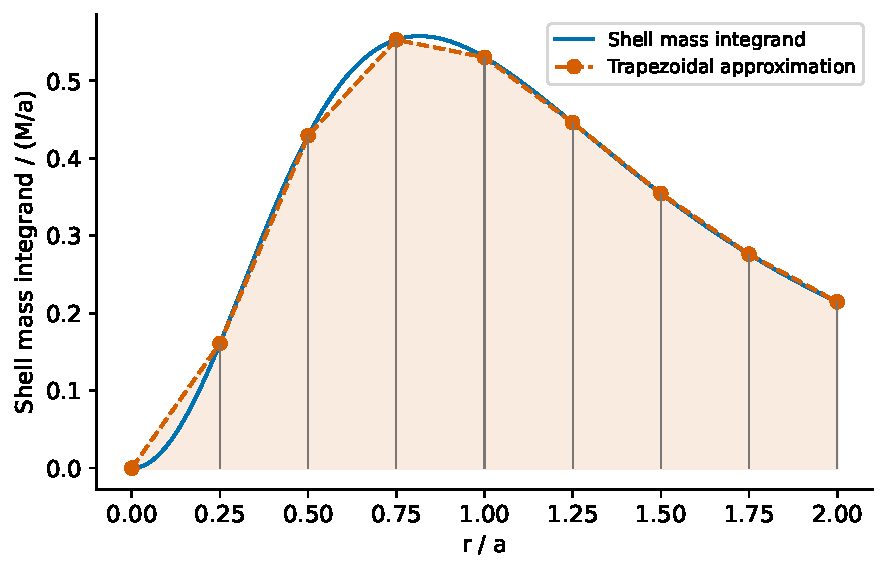
\includegraphics[width=118mm]{figures/ch03_trapezoid.pdf}};
  \begin{scope}[x={(plot.south east)},y={(plot.north west)}]
    \draw[figblue,line width=.85pt] (.645294,.181406) -- (.645294,.784836);
    \draw[figblue,line width=.85pt] (.744648,.181406) -- (.744648,.661074);
    \node[fill=white,inner sep=1.5pt,anchor=east,small label] (gl) at (.618,.64) {$g_j/(M/a)$};
    \draw[guide] (gl.east) -- (.645294,.770);
    \node[fill=white,inner sep=1.5pt,anchor=west,small label] (gr) at (.778,.48) {$g_{j+1}/(M/a)$};
    \draw[guide] (gr.west) -- (.744648,.645);
    \draw[{Latex[length=1.6mm]}-{Latex[length=1.6mm]},figblue] (.645294,.28) -- (.744648,.28);
    \node[small label,fill=white,inner sep=1pt,above] at (.694971,.29) {$\Delta r_j/a$};
  \end{scope}
\end{tikzpicture}

\caption{台形則で近似する球殻の質量の被積分関数。説明用に$0\leq r\leq2a$を8区間へ分けています。縦軸は$g/(M/a)=3(r/a)^2[1+(r/a)^2]^{-5/2}$です。標準の256区間の計算とは分割数が異なります。一つの台形の高さ$g_j,g_{j+1}$と幅$\Delta r_j$を注記しています。図の軸に合わせ、高さを$M/a$、幅を$a$で規格化しています。}
\label{fig:ch3-trapezoid}
\end{figure}

\subsection{各半径までの質量を順に足す}
すべての台形を最後に足すだけでなく、途中の和も保存します。数値積分で得た質量を$\widehat M_j$と書くと、
\begin{equation}
 \widehat M_0=0,\qquad
 \widehat M_{j+1}=\widehat M_j+\frac{g_j+g_{j+1}}{2}(r_{j+1}-r_j)
 \label{eq:ch3-cumulative-trapezoid}
\end{equation}
です。最後の値だけでなく、各分点に対応する累積質量の表が得られます。ハットはここでは数値近似を示すもので、無次元量を意味しません。

まずループで、式をそのまま実装します。
\inputcode{chap03/trapezoid}
\texttt{check\_grid}は、分点と関数値が同じ長さの1次元配列で、値が有限かつ分点が狭義単調増加していることを確認する補助関数です。実装はNotebookに置きます。積分の本体は、台形の面積を計算し、前の和へ足す2行です。

この関数へ、半径の表と$g$の値を渡します。
\inputcode{chap03/mass-table}
\texttt{mass\_numeric[j]}が$r_j$以内の質量です。\texttt{np.linspace}の最後の引数は分点数なので、区間数に1を加えます。

Notebookには、隣接する値をスライスで取り出し、\texttt{np.cumsum}で累積和を作る書き方も示します。計算している台形はループ版と同じです。まずは式と各配列要素の対応を理解し、コードが短いことだけを目標にしないようにします。

\subsection{2次精度の意味を確認する}
滑らかな関数について、一つの幅$\Delta r$の小区間を台形で近似した誤差は$O(\Delta r^3)$です。固定した範囲を等分すると、小区間の個数は$\Delta r^{-1}$に比例します。そのため、小区間の誤差を足した合成台形則の誤差は、通常$O(\Delta r^2)$になります。\cite{sugiura2009}

分割数を2倍にして幅を半分にすると、誤差がおよそ$1/4$になることを期待します。ただし、これは関数が滑らかで刻みが十分小さく、丸め誤差が支配しない範囲での話です。多項式を何次まで厳密に積分できるかという「代数的精度」とは、別の数え方です。本章では、\textbf{幅に対する誤差の変化}を確認します。

\begin{notebox}{ほかの数値積分法}
Simpson則は、小区間の関数を放物線で近似して積分する方法です。滑らかな問題では台形則より高い次数を得られます。Gauss求積のように、分点と重みの選び方を工夫する方法もあります。本章では、表から累積積分を作りやすい台形則を使います。ほかの方法の導出・実装は数値計算の教科書に譲ります。台形則とSimpson則の比較は、文献\cite{sugiura2009}の第3章を参照してください。
\end{notebox}

\Needspace{10\baselineskip}
\section{数値積分を解析式と比べる}
\label{sec:ch3-mass-check}
\subsection{原点でも使える誤差を定義する}
数値積分と解析式を同じ分点で比較します。原点では$M(<0)=0$なので、各半径の質量で割った相対誤差は使いません。球全体の質量$M$で規格化し、
\begin{equation}
 e_M=\max_{0\leq j\leq N_r}\frac{|\widehat M_j-M(<r_j)|}{M}
 \label{eq:ch3-mass-error}
\end{equation}
とします。これなら原点を含む表全体を、一つの基準で評価できます。

\begin{figure}[htbp]
\centering\includegraphics[width=0.72\linewidth]{\figpath{ch03_enclosed_mass}}
\caption{Plummer球の累積質量。灰色破線が解析式、青実線が$0\leq r\leq5a$を256区間で積分した結果です。両者はこの縮尺ではほぼ重なります。上の点線は球全体の質量であり、$5a$の内側だけでは到達しません。}
\label{fig:ch3-enclosed-mass}
\end{figure}

標準条件の最大誤差は$e_M=\chthreevalMassError$でした。図\ref{fig:ch3-enclosed-mass}がほぼ重なっても、この差は0ではありません。図の見た目とは別に、数値で確認することが必要です。

\subsection{積分範囲を固定して分割する}
ここでは$r_{\rm tab}=5a$を変えず、区間数$N_r$だけを増やします。
\inputcode{chap03/mass-convergence}
\begin{table}[htbp]
\centering
\caption{台形則の分割数試験。積分範囲は全行で$[0,5a]$です。$p_M$は前の行との誤差比から求めた推定次数で、最初の行には比較相手がありません。}
\label{tab:ch3-mass-convergence}
\begin{tabular}{rrrr}\toprule
$N_r$ & $\Delta r\ [\mathrm{kpc}]$ & $e_M$ & $p_M$ \\
\midrule
20 & 0.750000 & $5.87\times 10^{-3}$ & --- \\
40 & 0.375000 & $1.46\times 10^{-3}$ & 2.0037 \\
80 & 0.187500 & $3.76\times 10^{-4}$ & 1.9602 \\
160 & 0.093750 & $9.40\times 10^{-5}$ & 2.0014 \\
320 & 0.046875 & $2.35\times 10^{-5}$ & 2.0004 \\
\bottomrule\end{tabular}

\end{table}

推定次数は、第1・2章の時間刻みの試験と同様に、
\begin{equation}
 p_M=\frac{\log[e_M(\Delta r)/e_M(\Delta r/2)]}{\log2}
 \label{eq:ch3-mass-order}
\end{equation}
で求めます。表\ref{tab:ch3-mass-convergence}の最も細かい側では$p_M=\chthreevalMassOrder$となり、2次の収束を確認できます。最大誤差を取る分点の位置も分割数とともに変わるため、粗い側の推定次数が滑らかに2へ近づくとは限りません。

\begin{figure}[htbp]
\centering\includegraphics[width=0.70\linewidth]{\figpath{ch03_mass_convergence}}
\caption{半径方向の幅と質量誤差。点線は、最も細かい分割の実測値を通る傾き2の参照線です。実測点を当てはめて傾きを決めた線ではありません。}
\label{fig:ch3-mass-convergence}
\end{figure}

\subsection{積分範囲の効果と積分誤差を区別する}
同じ$[0,5a]$をいくら細かく分けても、得られるのは$M(<5a)$です。全質量$M$にはなりません。式\eqref{eq:ch3-mass-exact}から求めた、いくつかの範囲内の質量を表\ref{tab:ch3-cutoff}に示します。
\begin{table}[htbp]
\centering
\caption{有限半径の内側と外側の質量。すべて解析式の値です。範囲外にある質量と、有限刻みによる数値積分誤差を区別します。}
\label{tab:ch3-cutoff}
\begin{tabular}{rrr}\toprule
$r_{\rm tab}/a$ & $M(<r_{\rm tab})/M$ & 範囲外の質量$/M$ \\
\midrule
5 & 0.942866034 & 0.057133966 \\
10 & 0.985185337 & 0.014814663 \\
20 & 0.996261685 & 0.003738315 \\
\bottomrule\end{tabular}

\end{table}

例えば$5a$より外には、全質量の約5.7\%が残ります。これは台形則の失敗ではありません。全質量まで近づけたいときには積分範囲も広げます。ただし、区間数を固定したまま範囲だけ広げると、中心付近の分割が粗くなります。\textbf{範囲を広げることと、同じ範囲を細かく分けることは、別の操作です。}

\begin{failbox}{最後の値を無条件に全質量へそろえない}
\texttt{mass\_numeric[-1]}を$M$に合わせて表全体を再規格化すると、積分範囲の外の質量を内側へ配り直してしまいます。本章の$M$は無限遠まで含めた全質量です。有限半径で切断した別のモデルを作るときは、その定義を改めて示す必要があります。
\end{failbox}

\section{二分法で半質量半径を求める}
\label{sec:ch3-bisection}
\subsection{半径を未知数にする}
ここまでは半径を指定して、その内側の質量を求めました。次は、質量を指定して半径を求めます。\textbf{半質量半径}$r_h$は、球全体の質量の半分が入る半径です。
\begin{equation}
 M(<r_h)=\frac{M}{2}.
 \label{eq:ch3-half-definition}
\end{equation}

Plummerモデルでは、解析式を使って比較値も求められます。式\eqref{eq:ch3-mass-exact}を$M$で割って$1/2$と置き、両辺を$2/3$乗すると、
\[
 \frac{r_h^2}{r_h^2+a^2}=2^{-2/3}.
\]
これを$r_h$について整理すると、
\begin{equation}
 r_h=\frac{a}{\sqrt{2^{2/3}-1}}\simeq1.304766\,a
 \label{eq:ch3-half-exact}
\end{equation}
です。本章の$a=3\unit{kpc}$では$r_h=\chthreevalRhExact\unit{kpc}$です。今回も、この解析式だけで答えを出すのではなく、数値的な求め方を検証します。

\subsection{積分と求根を分ける}
二分法は、関数の値が0になる場所を探す\textbf{求根法}です。本章で計算する関数を
\begin{equation}
 F(r)=\frac{\widehat M(<r)}{M}-\frac12
 \label{eq:ch3-root-function}
\end{equation}
とします。$\widehat M$は台形則の結果です。$F<0$なら内側の質量が半分より少なく、$F>0$なら多いことを意味します。

先ほどの質量表は決まった分点の値だけを持っていますが、二分法ではその間の半径も試します。そこで本章では、\textbf{半径を試すたびに$[0,r]$を同じ区間数で積分し直す}実装にします。表の補間をまだ必要とせず、二分法が呼ぶ関数の意味を直接追えます。
\inputcode{chap03/mass-at-radius}

\texttt{enclosed\_mass\_trapezoid}は積分、\texttt{half\_mass\_residual}は求根する方程式を担当します。$r=0$なら積分値は0として返します。$r>0$では、区間幅は$r/N_r$です。求根の途中では$r$が変わるので、分割幅も変わります。

\subsection{符号の変わる区間を半分にする}
連続な関数$F$について、端点$r_L<r_U$で符号が異なれば、その間に少なくとも一つの根があります。Plummer球の真の累積質量は単調増加するので、半質量半径は一つです。標準の数値積分でも、$[0,5a]$の両端で$F(0)<0$、$F(5a)>0$になります。

まず中点を計算します。
\begin{equation}
 r_C=\frac{r_L+r_U}{2}.
 \label{eq:ch3-bisection}
\end{equation}
$F(r_C)$が$F(r_L)$と同符号なら、根は右半分にあるので$r_L\leftarrow r_C$とします。異符号なら左半分を残し、$r_U\leftarrow r_C$とします。これを繰り返すのが二分法です。導関数は必要ありません。\cite{sugiura2009}

根が残る側を選んでいるので、区間の幅は毎回半分になります。ただし、符号が変わるだけで十分なのは、関数がその区間で連続な場合です。不連続な発散点を挟んで符号が違っても、そこに根があるとは限りません。


% BEGIN TikZ addition: ch03_bisection
図\ref{fig:concept-ch3-bisection}で、端点と中点の符号から、次に残す半区間をたどってください。太い線の範囲が次の行の探索区間になります。
\begin{figure}[!htbp]
\centering
% Standard [0,5a] bracket: signs correspond to the chapter's half-mass function.
% r_* denotes the root of the function actually evaluated, not an error-free physical radius.
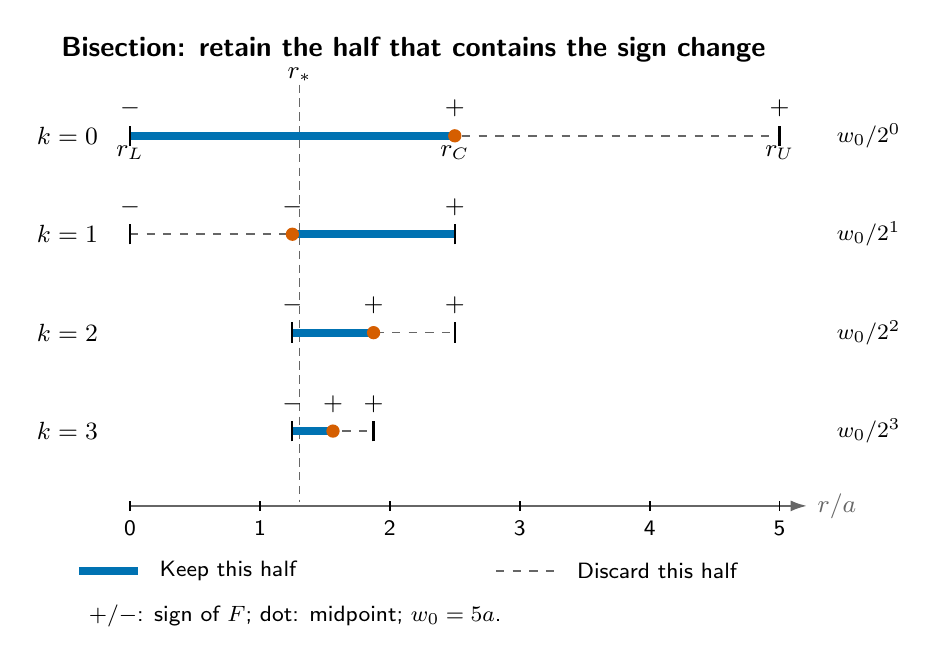
\begin{tikzpicture}[textbook diagram,x=1cm,y=1cm]
  \node[anchor=west,font=\sffamily\bfseries] at (0,1.10) {Bisection: retain the half that contains the sign change};
  \draw[guide] (3.153,0.65) -- (3.153,-4.65);
  \node[above,fill=white,inner sep=1pt] at (3.153,0.65) {$r_*$};
  \foreach \k/\y/\lo/\mid/\hi/\keepL/\keepU/\sign in {
    0/0/0/2.5/5/0/2.5/+,
    1/-1.25/0/1.25/2.5/1.25/2.5/-,
    2/-2.5/1.25/1.875/2.5/1.25/1.875/+,
    3/-3.75/1.25/1.5625/1.875/1.25/1.5625/+} {
    \node[anchor=east] at (.72,\y) {$k=\k$};
    \draw[figgray,dashed] ({1+1.65*\lo},\y) -- ({1+1.65*\hi},\y);
    \draw[figblue,line width=3pt] ({1+1.65*\keepL},\y) -- ({1+1.65*\keepU},\y);
    \foreach \p in {\lo,\hi} {\draw[line width=0.8pt] ({1+1.65*\p},{\y-.13}) -- ({1+1.65*\p},{\y+.13});}
    \fill[figred] ({1+1.65*\mid},\y) circle (2.4pt);
    \node[above,inner sep=3pt] at ({1+1.65*\lo},{\y+.12}) {$-$};
    \node[above,inner sep=3pt] at ({1+1.65*\mid},{\y+.12}) {$\sign$};
    \node[above,inner sep=3pt] at ({1+1.65*\hi},{\y+.12}) {$+$};
    \node[anchor=west,small label] at (9.85,\y) {$w_0/2^{\k}$};
  }
  \node[below] at (1,0) {$r_L$};
  \node[below] at (5.125,0) {$r_C$};
  \node[below] at (9.25,0) {$r_U$};
  \draw[vector,figgray] (1,-4.70) -- (9.6,-4.70) node[right] {$r/a$};
  \foreach \x in {0,1,2,3,4,5} {\draw ({1+1.65*\x},-4.64) -- ({1+1.65*\x},-4.77);\node[below,small label] at ({1+1.65*\x},-4.77) {\x};}
  \draw[figblue,line width=3pt] (0.35,-5.53) -- (1.1,-5.53);
  \node[anchor=west,small label] at (1.25,-5.53) {Keep this half};
  \draw[figgray,dashed] (5.65,-5.53) -- (6.4,-5.53);
  \node[anchor=west,small label] at (6.55,-5.53) {Discard this half};
  \node[small label,anchor=west] at (0.35,-6.10) {$+/-$: sign of $F$; dot: midpoint; $w_0=5a$.};
\end{tikzpicture}

\caption{初期区間$[0,5a]$からの二分法の例。点が中点、$+,-$が評価した$F$の符号、太い線が次に残す半区間です。$k$はそれまでの半減回数です。破線$r_*$は評価している数値関数の根であり、元の密度の真の半質量半径と必ずしも一致しません。}
\label{fig:concept-ch3-bisection}
\end{figure}
\FloatBarrier
% END TikZ addition: ch03_bisection

\subsection{二分法の終了条件を決める}
初期区間の幅を$w_0$とします。$k$回区間を半分にした後の幅は$w_k=w_0/2^k$です。その区間の中点を根の近似値とすれば、区間が正しい根を含む限り、中点から根までの距離は半区間幅以下です。
\begin{equation}
 |r_C-r_\ast|\leq\frac{w_k}{2}=\frac{w_0}{2^{k+1}}.
 \label{eq:ch3-root-bound}
\end{equation}
ここで$r_\ast$は、\textbf{実際に評価している関数$F$の根}です。まだ、元の連続的な密度の真の半質量半径$r_h$と同じとは限りません。

本章では、半区間幅が許容値$\tau_r$以下になったら終了します。$\tau_r$は半径と同じ単位を持ちます。例えば\texttt{root\_xtol = 1e-8}は$10^{-8}\unit{kpc}$です。無次元の残差$|F|$の許容値ではありません。

符号を保つ更新をコードにします。
\inputcode{chap03/bisection}

\texttt{check\_bisection}は、区間、許容幅、反復回数、端点の符号を確認します。\texttt{finite\_value}は、関数値が有限であることを確認します。両者の完全なコードはNotebookに含めます。\texttt{np.signbit}は負の符号を持つかどうかを返し、関数値どうしの積を作らずに同符号かを判定できます。

\texttt{trace}には、反復番号、左右の端点、中点、残差、半区間幅を保存します。関数値が計算上ちょうど0になった場合も終了します。通常の浮動小数点演算を使うため、これは丸めを含めて厳密に根を保証する区間演算の実装ではありません。更新が丸めの限界に達したときや反復上限を超えたときには、未収束として停止します。

\subsection{実際に半質量半径を求める}
\inputcode{chap03/half-mass}
標準の256区間では、数値結果は$\widehat r_h=\chthreevalRh\unit{kpc}$でした。区間を半分にした回数は\chthreevalRootHalvings 回、中点を評価した回数は\chthreevalRootCalls 回です。最初の区間の中点も評価しているため、二つの回数は1だけ異なります。終了時の半区間幅は$\chthreevalRootWidth\unit{kpc}$です。

\begin{notebox}{ほかの求根法}
Newton法は関数値と導関数から次の近似値を決め、適切な条件では二分法より速く収束しますが、初期値や関数の性質に注意が必要です。割線法は導関数の代わりに二つの点から傾きを見積もります。Brent法は区間を保つ操作と補間を組み合わせる方法です。本章では、根を挟む区間を追いやすい二分法に集中します。二分法、Newton法、割線法は文献\cite{sugiura2009}の第9章を参照してください。Brent法など、ここで扱わない方法の詳細は数値計算の専門書に譲ります。
\end{notebox}

\section{求根の残差と半径の誤差を区別する}
\label{sec:ch3-root-errors}
\subsection{二つの誤差を区別する}
二分法を終えたときの$|F(\widehat r_h)|$は$\chthreevalRootResidual$でした。一方、同じ半径を解析的な質量式へ代入したときの残差は、
\[
 \left|\frac{M(<\widehat r_h)}{M}-\frac12\right|=\chthreevalTrueResidual
\]
です。二つの値は一致しません。二分法は台形則で定義した$F$を0へ近づけていますが、その$F$自体に積分の誤差が含まれるためです。

実際、真の半径との差は$|\widehat r_h-r_h|=\chthreevalRhError\unit{kpc}$で、二分法の最終半区間幅より大きくなっています。式\eqref{eq:ch3-root-bound}が誤っているのではありません。そこに現れる$r_\ast$が、台形則で作った関数の根だからです。

\subsection{まず積分の分割数を変える}
求根の初期区間と許容幅を固定し、質量積分の区間数だけを変えます。
\inputcode{chap03/root-convergence}
\begin{table}[htbp]
\centering
\caption{積分の区間数による半質量半径の変化。二分法の許容半区間幅は全行で$10^{-8}\unit{kpc}$です。小さな数値残差が得られていても、真の半径との差には区間数への依存が残ります。}
\label{tab:ch3-root-convergence}
\small\begin{tabular}{rrrr}\toprule
$N_r$ & $\widehat r_h\ [\mathrm{kpc}]$ & $|\widehat r_h-r_h|\ [\mathrm{kpc}]$ & $|F(\widehat r_h)|$ \\
\midrule
32 & 3.914664479 & $3.66\times 10^{-4}$ & $7.95\times 10^{-10}$ \\
64 & 3.914389650 & $9.16\times 10^{-5}$ & $5.68\times 10^{-10}$ \\
128 & 3.914320974 & $2.29\times 10^{-5}$ & $3.60\times 10^{-10}$ \\
256 & 3.914303805 & $5.73\times 10^{-6}$ & $3.93\times 10^{-10}$ \\
512 & 3.914299516 & $1.44\times 10^{-6}$ & $8.84\times 10^{-10}$ \\
\bottomrule\end{tabular}

\end{table}

表\ref{tab:ch3-root-convergence}では、積分を細かくすると真の半径との差も小さくなります。本例では、その差はおよそ区間数の2乗に反比例して減っています。求根の終了条件を厳しくする前に、その関数値をどの精度で計算しているかを見る必要があります。

\subsection{次に求根の許容幅だけを変える}
今度は積分を64区間に固定し、$\tau_r$だけを変えます。
\begin{table}[htbp]
\centering
\caption{積分を64区間に固定した許容幅の試験。求根を細かく続けても、積分から来る半径のずれは取り除けません。}
\label{tab:ch3-root-tolerance}
\small\begin{tabular}{rrrr}\toprule
$\tau_r\ [\mathrm{kpc}]$ & 最終半区間幅$\ [\mathrm{kpc}]$ & 真の半径との差$\ [\mathrm{kpc}]$ & $|F|$ \\
\midrule
$1.00\times 10^{-2}$ & $7.32\times 10^{-3}$ & $4.16\times 10^{-3}$ & $5.76\times 10^{-4}$ \\
$1.00\times 10^{-4}$ & $5.72\times 10^{-5}$ & $9.63\times 10^{-5}$ & $6.70\times 10^{-7}$ \\
$1.00\times 10^{-6}$ & $8.94\times 10^{-7}$ & $9.18\times 10^{-5}$ & $3.61\times 10^{-8}$ \\
$1.00\times 10^{-8}$ & $6.98\times 10^{-9}$ & $9.16\times 10^{-5}$ & $5.68\times 10^{-10}$ \\
\bottomrule\end{tabular}

\end{table}

許容幅が十分小さくなると、真の半径との差は約$\chthreevalRootFloor\unit{kpc}$の付近でほぼ変わらなくなります。これは計算機の丸め誤差まで到達したからではなく、この実験では質量積分の誤差が残っているからです。

\begin{figure}[htbp]
\centering\includegraphics[width=0.73\linewidth]{\figpath{ch03_bisection_errors}}
\caption{64区間の質量積分を使った二分法の履歴。青は半区間幅、朱色は中点と解析的な半質量半径の差です。半区間幅は半減を続けますが、真の半径との差は積分誤差の大きさ付近に残ります。どちらも$a$で規格化しています。}
\label{fig:ch3-bisection-errors}
\end{figure}

\begin{failbox}{求根の桁数だけで結果の精度を判断しない}
数値的な関数の残差が小さくても、もとの方程式を同じ精度で解けたとは限りません。積分の分割数と求根の許容幅を別々に変更して確認します。また、$M/2$を$\widehat M(<r_{\rm tab})/2$へ替えると、有限の範囲内にある質量の半分を求める、別の問題になります。
\end{failbox}

\section{Plummer球の重力で星を動かす}
\label{sec:ch3-orbit}
\subsection{加速度は解析式から与える}
ここからは、星を表す1粒子の時間発展を計算します。質量積分と求根の誤差を軌道へ混ぜないため、\textbf{本章の標準軌道計算には解析的なPlummer加速度を使います。}数値的な質量表は、ここまでの積分・求根の学習と検証に使ったものです。

式\eqref{eq:ch3-potential}を微分すると、
\[
 \frac{d\Phi}{dr}=\frac{GM r}{(r^2+a^2)^{3/2}}
\]
なので、加速度は
\begin{equation}
 \boxed{\avec(\rvec)=-\frac{GM\rvec}{(r^2+a^2)^{3/2}}}
 \label{eq:ch3-acceleration}
\end{equation}
です。これは式\eqref{eq:ch3-enclosed-force}へ解析的な$M(<r)$を代入しても得られます。二つの求め方が一致することが、密度・質量・ポテンシャルの整合性の確認になります。

原点では$\avec=0$です。$r\ll a$では
\begin{equation}
 \avec\simeq-\frac{GM}{a^3}\rvec,
 \label{eq:ch3-inner-force}
\end{equation}
となり、位置に比例する調和振動子の形になります。一方、$r\gg a$では点質量の重力へ近づきます。中心で加速度が発散しないのは、質量分布を広げたモデルの性質であり、計算エラーを隠す処置ではありません。

\subsection{円運動速度も同じモデルから求める}
式\eqref{eq:ch3-vc-general}に代入すると、
\begin{equation}
 v_c^2(r)=\frac{GMr^2}{(r^2+a^2)^{3/2}},\qquad
 \Omega_c(r)=\frac{v_c(r)}{r}
 \label{eq:ch3-circular-speed}
\end{equation}
です。$r>0$の円軌道周期は$T_c(r)=2\pi/\Omega_c(r)$になります。中心近くでは$v_c\propto r$、十分外では$v_c\propto r^{-1/2}$です。\cite{bt2008}

\begin{figure}[htbp]
\centering\includegraphics[width=0.72\linewidth]{\figpath{ch03_circular_speed}}
\caption{同じ全質量を持つPlummer球と点質量の円運動速度。丸は本章の初期半径$r_0=2a$です。点質量の曲線は$r\geq0.5a$だけを示しています。原点に向かって発散する点質量の速度と、中心で0へ向かうPlummer球の速度は異なります。}
\label{fig:ch3-circular-speed}
\end{figure}

まずは成分で加速度を計算します。
\inputcode{chap03/acceleration-scalar}
本章の初期位置では$\avec\simeq(\chthreevalAccelX,0)\unit{kpc\,Gyr^{-2}}$です。この計算を短い関数にします。
\inputcode{chap03/acceleration-plummer}
\texttt{pos}と返り値は、1粒子なので形が\texttt{(1, 2)}です。多数の粒子への一般化は、第4章で行います。円運動速度の関数では、半径ごとの表を描けるよう配列も受け取ります。

\begin{failbox}{点質量の円運動速度を流用しない}
Plummer球の内部では、全質量$M$を使った$\sqrt{GM/r}$は円運動速度ではありません。力のモデルを変えたら、初期速度も同じモデルから計算し直します。$a$を変えて円軌道を比較するときも同様です。
\end{failbox}

\section{KDKで円軌道と非円軌道を計算する}
\label{sec:ch3-kdk}
\subsection{変える初期値を一つにする}
初期半径を$r_0=2a=6\unit{kpc}$とし、初期位置と速度を
\begin{equation}
 \rvec(0)=(r_0,0),\qquad \vvec(0)=(0,\eta v_c(r_0))
 \label{eq:ch3-initial}
\end{equation}
と置きます。$\eta=1$が円軌道、$\eta=0.7$が比較する非円軌道です。どちらも動径方向の初期速度は0で、反時計回りに動き始めます。

$0<\eta<1$では、円運動を保つために必要な接線速度より遅いため、初期半径から内側へ動き始めます。この初期位置は遠点です。ただし、第2章のKepler問題とは違い、その後の軌道は一般には閉じた楕円になりません。\textbf{非円軌道を最初から「楕円」と呼ばない}ようにします。

\inputcode{chap03/orbit-parameters}
\begin{table}[htbp]
\centering
\caption{本章の標準軌道条件。二つのケースで共通の基準周期$T_c$を使います。これは非円軌道の動径振動の周期を表す記号ではありません。}
\label{tab:ch3-parameters}
\begin{tabular}{ll}\toprule
量 & 設定または計算値\\\midrule
$M$, $a$ & $10^{11}\Msun$, $3\unit{kpc}$\\
$r_0$ & $6\unit{kpc}=2a$\\
$v_c(r_0)$ & $\chthreevalVc\unit{km\,s^{-1}}$\\
$T_c=2\pi r_0/v_c(r_0)$ & $\chthreevalTc\unit{Gyr}$\\
$\eta$ & $1$, $0.7$\\
$t_{\rm end}$ & $5T_c=\chthreevalTend\unit{Gyr}$\\
$N_{\rm step}$, $\Delta t$ & $5000$, $T_c/1000=\chthreevalDt\unit{Myr}$\\\bottomrule
\end{tabular}
\end{table}

初期状態を作る関数は、位置と速度を横につないだ\texttt{(1, 4)}の配列を返します。
\inputcode{chap03/initial-state}
\texttt{check\_model}は、$M$と$a$が有限かつ正であることを確認する関数です。KDKでは、まとめた状態から位置と速度を分けて取り出し、更新します。

\subsection{前章の積分法を再利用する}
KDKの計算は、半ステップの速度更新、1ステップの位置更新、新しい位置での加速度評価、残りの半ステップの速度更新です。
\inputcode{chap03/leapfrog-step}
前章から変えたのは、重力の関数へ渡すパラメータです。今回は二つの質量の配列ではなく、1個の銀河の\texttt{mass}と\texttt{a}を渡します。KDKの4行と、最後の加速度を再利用する構造は同じです。

\inputcode{chap03/integrate-leapfrog}
\texttt{prepare\_history}は、初期値をコピーし、時刻の配列と保存領域を作る補助関数です。前章と同じ役割ですが、今回は初期状態が\texttt{(1, 4)}であることを確認します。履歴は\texttt{(n\_steps + 1, 1, 4)}です。保存する速度は、最後の半ステップの更新を終えた整数時刻の値です。

5000ステップなら、加速度関数の評価は初回を含めて5001回です。台形則の区間数や二分法の反復回数は、この回数に含めません。いま評価している重力には解析式を使っています。

\subsection{同じ時間まで独立に計算する}
\inputcode{chap03/run-orbits}
一つのケースの最終状態を、別のケースの初期状態に流用しません。いずれも式\eqref{eq:ch3-initial}から作り直します。実行時間は環境に依存するので、Notebookで\texttt{perf\_counter}を使って測ります。

\begin{figure}[htbp]
\centering\includegraphics[width=0.70\linewidth]{\figpath{ch03_orbits}}
\caption{静的なPlummer球中の円軌道と非円軌道。青実線が$\eta=1$、朱色破線が$\eta=0.7$で、どちらも$5T_c$まで計算しています。中心の十字はポテンシャルの中心であり、追加した点質量ではありません。丸が共通の初期位置です。}
\label{fig:ch3-orbits}
\end{figure}

円軌道では半径がほぼ一定ですが、非円軌道では半径が増減し、近点・遠点の方向も変わります。このような軌道はロゼット軌道と呼ばれます。球対称でも、動径方向の振動と方位角方向の回転が、Kepler問題と同じ周期関係になるとは限りません。\cite{bt2008} 数値誤差による軌道のずれと区別するため、後で時間刻みを細かくした結果も比べます。

Notebookには、保存済みの履歴を使うアニメーションも含めます。画面上の再生間隔は物理的な時間刻みとは別で、動画の速度を変えても数値軌道は変わりません。

\Needspace{10\baselineskip}
\section{保存量と時間刻みを確認する}
\label{sec:ch3-validation}
\subsection{確認するエネルギーを決める}
固定した銀河ポテンシャル中のテスト粒子なので、確認するのは粒子の\textbf{単位質量当たり}のエネルギーと角運動量です。
\begin{equation}
 \varepsilon=\frac12(v_x^2+v_y^2)-\frac{GM}{\sqrt{r^2+a^2}},\qquad
 \ell_z=xv_y-yv_x.
 \label{eq:ch3-invariants}
\end{equation}
$\Phi$は時間に依存しないので、
\[
 \frac{d\varepsilon}{dt}=\vvec\cdot\avec+\nabla\Phi\cdot\vvec=0
\]
です。力は中心向きなので、$d\ell_z/dt=x a_y-y a_x=0$でもあります。第2章の二つの質量を掛けた全エネルギーや、Plummer球自身の自己重力エネルギーを計算しているわけではありません。

\inputcode{chap03/diagnostics}
位置と速度を同じ保存時刻から取り出します。Plummerポテンシャルを使って運動した結果に、点質量の$-GM/r$を足してエネルギーを診断しないようにします。

\subsection{有限刻みによる差を測る}
今回の2例では$\varepsilon(0)$と$\ell_z(0)$がともに0ではないので、その絶対値で規格化できます。保存した全時刻での最大値を
\begin{equation}
 e_\varepsilon=\max_n\frac{|\varepsilon^n-\varepsilon^0|}{|\varepsilon^0|},\qquad
 e_\ell=\max_n\frac{|\ell_z^n-\ell_z^0|}{|\ell_z^0|}
 \label{eq:ch3-invariant-errors}
\end{equation}
とします。初期値が0の別の軌道では、この規格化は使わず、第2章のように正の基準量を選ぶ必要があります。

\begin{table}[htbp]
\centering
\caption{標準条件の保存量と最小保存半径。両例とも$5T_c$まで5000ステップで計算しています。角運動量の末尾の桁は実行環境で多少変わります。}
\label{tab:ch3-conservation}
\small\begin{tabular}{lrrr}\toprule
軌道 & $e_\varepsilon$ & $e_\ell$ & 保存された最小半径$\ [\mathrm{kpc}]$ \\
\midrule
円 & $1.62\times 10^{-10}$ & $1.08\times 10^{-14}$ & 6.000000 \\
非円 & $1.83\times 10^{-5}$ & $9.47\times 10^{-15}$ & 3.027208 \\
\bottomrule\end{tabular}

\end{table}

\begin{figure}[htbp]
\centering\includegraphics[width=0.73\linewidth]{\figpath{ch03_energy}}
\caption{粒子の比エネルギーの初期値からの符号付きの差。円軌道の差は小さく、この縮尺では0付近に重なります。非円軌道では半径の増減に伴い差が変動します。これは摩擦によるエネルギー損失を入れた計算ではありません。}
\label{fig:ch3-energy}
\end{figure}

KDKでは中心力によるkickも、速度を固定するdriftも角運動量を保つため、$e_\ell$は丸め誤差程度になります。一方、エネルギーを毎ステップ厳密に保つ方法ではないので、円軌道では$e_\varepsilon=\chthreevalCircEnergy$、非円軌道では$\chthreevalNoncEnergy$という有限の差が現れました。保存量が小さくずれることと、軌道上の位置が同じ精度で正しいことは、別に調べます。

\subsection{円軌道を同じ時刻の解析位置と比べる}
円軌道では、$\Omega_c=v_c(r_0)/r_0$から解析的な位置を
\begin{equation}
 \rvec_{\rm exact}(t)=r_0(\cos\Omega_c t,\sin\Omega_c t)
 \label{eq:ch3-circle-exact}
\end{equation}
と書けます。同じ時刻の数値解との最大の距離を、初期半径で規格化します。
\begin{equation}
 e_r=\max_n\frac{|\rvec^n-\rvec_{\rm exact}(t_n)|}{r_0}.
 \label{eq:ch3-position-error}
\end{equation}
半径の差だけではないので、回転の位相がずれた場合も検出できます。

この試験だけ最終時刻を$T_c$とし、100、200、400、800ステップで比較します。$5T_c$の標準図とは計算時間が異なりますが、試験系列の中では同じ時刻まで計算します。
\inputcode{chap03/orbit-convergence}

\begin{table}[htbp]
\centering
\caption{Plummer球中の円軌道の時間刻み試験。最終時刻は全行で解析的な円軌道周期$T_c$です。$p_r$は前の行との位置誤差の比から求めます。}
\label{tab:ch3-orbit-convergence}
\begin{tabular}{rrrr}\toprule
$N_{\rm step}$ & $\Delta t\ [\mathrm{Myr}]$ & $e_r$ & $p_r$ \\
\midrule
100 & 1.627630 & $3.25\times 10^{-3}$ & --- \\
200 & 0.813815 & $8.12\times 10^{-4}$ & 2.00052 \\
400 & 0.406907 & $2.03\times 10^{-4}$ & 2.00020 \\
800 & 0.203454 & $5.07\times 10^{-5}$ & 2.00005 \\
\bottomrule\end{tabular}

\end{table}

\begin{figure}[htbp]
\centering\includegraphics[width=0.72\linewidth]{\figpath{ch03_orbit_convergence}}
\caption{Plummer球中の円軌道に対する位置誤差。横軸は$\Delta t/T_c$です。点線は、最も細かい刻みの実測点を通る傾き2の参照線です。}
\label{fig:ch3-orbit-convergence}
\end{figure}

最も細かい側の推定次数は$p_r=\chthreevalOrbitOrder$で、KDKの2次精度を確認できました。重力場を点質量からPlummer球へ変えても、滑らかな軌道を十分小さい刻みで追う場合の次数は同じです。円軌道のエネルギー誤差には特殊な打ち消しが生じる場合があるので、その誤差だけから解法の次数を判断しません。

\subsection{閉じない非円軌道の精度を確かめる}
非円軌道では、$T_c$や$5T_c$後に初期位置へ戻るとは限りません。初期位置へ戻らない量を、そのまま誤差にしてはいけません。本章では、同じ$5T_c$まで異なる刻みで計算した終点を比較します。

刻み$h$と$h/2$による終点を使い、
\begin{equation}
 d_h=\frac{|\rvec_h(t_{\rm end})-\rvec_{h/2}(t_{\rm end})|}{r_0}
 \label{eq:ch3-self-convergence}
\end{equation}
とします。もし$\rvec_h=\rvec_{\rm true}+\boldsymbol C h^2+\cdots$で主要な誤差を表せるなら、差を取ると$(3/4)\boldsymbol C h^2$が残るので、$d_h/d_{h/2}$は約4になります。

\begin{table}[htbp]
\centering
\caption{非円軌道の終点の自己収束試験。すべて$5T_c$まで計算します。各行は、隣接する二つの刻みの数値解の差です。真の解との誤差ではありません。}
\label{tab:ch3-noncircular}
\small\begin{tabular}{rrrr}\toprule
粗い計算のステップ数 & 細かい計算のステップ数 & 終点の差$/r_0$ & 前の行との比 \\
\midrule
1250 & 2500 & $8.98\times 10^{-4}$ & --- \\
2500 & 5000 & $2.25\times 10^{-4}$ & 3.99969 \\
5000 & 10000 & $5.61\times 10^{-5}$ & 3.99992 \\
\bottomrule\end{tabular}

\end{table}

細かい側の比は\chthreevalNoncRatio で、およそ4でした。図\ref{fig:ch3-orbits}のロゼット状の運動が、刻みを細かくするとKepler楕円へ変わるわけではありません。ただし、自己収束の確認だけで、力の式そのものが正しいと証明できるわけでもありません。解析的な円軌道、密度と力の関係、保存量と合わせて判断します。

\section{三つの数値計算の役割を区別する}
\label{sec:ch3-error-budget}
ここまでの計算では、同じPlummerモデルに対して、異なる目的の算法を使いました。どの入力を変えると、どの誤差を調べることになるかを整理しておきます。

\begin{center}
\begin{tabularx}{\linewidth}{lXX}\toprule
操作 & 固定するもの & 確認するもの\\\midrule
台形則の区間を細かくする & 積分範囲、密度モデル & 解析的な質量との差\\
二分法の許容幅を小さくする & 質量積分の区間数、求根区間 & 数値的な関数の根の精度\\
KDKの時間刻みを小さくする & 初期条件、重力場、最終時刻 & 軌道位置と保存量の変化\\\bottomrule
\end{tabularx}
\end{center}

$a$を変えることは、これらの数値精度を調整することとは違います。密度分布と重力そのものを変更する、\textbf{物理モデルの変更}です。例えば$M$と$r_0$を固定して$a$を大きくすると、内側の質量が減り、円運動速度は小さくなります。円軌道を比較するのか、同じ位置・速度から異なるポテンシャルでの応答を比べるのかによって、そろえる初期条件も変わります。

また、本章では軌道に解析的な力を使っているので、台形則の区間数を変えても、そのまま軌道の計算結果が変わることはありません。数値的な質量表から力を計算する実装へ拡張した場合には、空間の積分・補間誤差と時間積分誤差を、改めて分けて確かめる必要があります。そこまでの拡張は本章の必須課題にはしません。

\section{本章のまとめ}
\label{sec:ch3-summary}
本章では、質量に広がりを持つ静的な銀河を、球対称のPlummerモデルで表しました。密度を球殻の体積で重み付けして積分すると、内側の質量が得られます。球対称の重力加速度と円運動速度は、その内側の質量から決まります。一方、ポテンシャルには外側の質量も寄与するため、力と同じ置き換えを無条件に行いません。

台形則では、小区間の両端を結ぶ直線の下の面積を足しました。積分範囲を固定して幅を半分にすると、質量の誤差がおよそ$1/4$になることを確認しました。二分法では、半質量半径を挟む区間を保って半分にしました。ただし、二分法の残差を小さくしても、関数値に含まれる質量積分の誤差までは消えません。

最後に、解析的なPlummer加速度をKDKへ渡して、円軌道と非円軌道を計算しました。固定した球対称場では、粒子の比エネルギーと比角運動量を確認できます。円軌道の解析位置と、非円軌道の刻みを変えた比較も使い、保存量だけに頼らず結果を確かめました。

次の第4章では、1個のテスト粒子から多数の粒子へ進みます。円盤上の分布を作るために、台形則による累積積分を再利用し、線形補間と乱数を組み合わせます。見た目に円盤状の粒子を配置しても、その粒子自身の自己重力を計算するわけではない、という区別を引き継ぎます。

\chapterexercises
\paragraph{演習3.1　確認：密度・質量・円運動速度}
$M=10^{11}\Msun$、$a=3\unit{kpc}$について、中心密度$\rho(0)$、$M(<a)/M$、半質量半径$r_h$を計算してください。また、$r=2a$での円運動速度を$\mathrm{km\,s^{-1}}$と内部単位の両方で示してください。軌道を2次元で計算する場合でも、質量積分に$4\pi r^2$が必要な理由を説明してください。

\paragraph{演習3.2　確認：台形則の配列}
$[0,5a]$を$N_r=40$区間に分けたときの分点数と区間幅を求めてください。\texttt{cumulative\_trapezoid}のループで、\texttt{integral[j + 1]}が何を表すか説明してください。密度ではなく$g=4\pi r^2\rho$を渡す理由を、単位からも確かめてください。

\paragraph{演習3.3　応用：範囲と分割数を分ける}
$[0,5a]$の区間数を増やす実験と、$\Delta r$を固定して範囲を$5a,10a,20a$へ広げる実験を行ってください。数値積分の誤差と範囲外の質量を別々に示してください。全質量$M$と$M(<5a)$の違いを、台形則の誤差だけで説明できるでしょうか。

\paragraph{演習3.4　確認：二分法の反復回数}
初期区間を$[0,15]\unit{kpc}$としたとき、半区間幅を$10^{-8}\unit{kpc}$以下にするには何回の半減が必要か求めてください。半減回数と中点評価回数の違いも示してください。また、$|F(\widehat r_h)|$が小さくても、$|\widehat r_h-r_h|$が同じ程度には小さくならない理由を説明してください。

\paragraph{演習3.5　応用：球全体の半分と、範囲内の半分}
求根式の右辺を$M/2$から$M(<5a)/2$へ変えて、二つの半径を比較してください。先に解析式で違いを確認し、その後、数値積分で作る関数を二分法で解いてください。どちらが小さくなるでしょうか。この変更が単なる数値精度の改善ではない理由を述べてください。

\paragraph{演習3.6　応用：スケール長を変える}
$M$と$r_0=6\unit{kpc}$を固定し、$a=1.5,3,6\unit{kpc}$の円運動速度と半質量半径を求めてください。それぞれに対応する円運動速度で初期条件を作り、円軌道を計算してください。すべてに同じ初期速度を与えた場合とは、何を比較している点が違うでしょうか。

\paragraph{演習3.7　発展：非円軌道の近点を求根で調べる}
$\eta=0.7$の初期比エネルギー$\varepsilon_0$、比角運動量$\ell_{z,0}$を用いて、
\begin{equation}
 \Phi(r)+\frac{\ell_{z,0}^2}{2r^2}-\varepsilon_0=0
 \label{eq:ch3-turning-point}
\end{equation}
の根を二分法で求めてください。この式は、動径速度が0になる条件です。初期遠点$r_0$ではない内側の根を探すため、区間を$[0.05r_0,0.95r_0]$とします。関数の符号を確認してから求根し、軌道の保存された最小半径と比較してください。両者の違いには何が含まれるでしょうか。

\newcommand{\chfourvalCq}{0.959572318}
\newcommand{\chfourvalNodeError}{9.29\times 10^{-8}}
\newcommand{\chfourvalInverseError}{1.76\times 10^{-7}}
\newcommand{\chfourvalHalfInterp}{4.843929332}
\newcommand{\chfourvalHalfExact}{4.843928453}
\newcommand{\chfourvalHalfSample}{4.782418}
\newcommand{\chfourvalFractionRd}{0.275373844}
\newcommand{\chfourvalMinRadius}{0.100153}
\newcommand{\chfourvalMaxRadius}{14.950926}
\newcommand{\chfourvalSampleError}{0.029414}
\newcommand{\chfourvalFinalCDF}{0.029420}
\newcommand{\chfourvalVectorDiff}{7.28\times 10^{-17}}
\newcommand{\chfourvalCorePeriod}{48.677}
\newcommand{\chfourvalPosError}{5.46\times 10^{-4}}
\newcommand{\chfourvalRadiusError}{4.73\times 10^{-5}}
\newcommand{\chfourvalEnergyError}{2.19\times 10^{-9}}
\newcommand{\chfourvalAngularError}{5.00\times 10^{-14}}
\newcommand{\chfourvalOrbitOrder}{2.00004}
\newcommand{\chfourvalReverseError}{5.46\times 10^{-4}}
\newcommand{\chfourvalSubMedian}{4.025966}
\newcommand{\chfourvalSubEnergy}{1.55\times 10^{-5}}
\newcommand{\chfourvalAllMemory}{96.032}
\newcommand{\chfourvalSavedMemory}{9.632}
\newcommand{\chfourvalMemorySeries}{96.032,9.632,1.952}
\newcommand{\chfourvalSavedSeries}{3001,301,61}
\newcommand{\chfourvalPlummerHalf}{3.9143}

\chapter{テスト粒子で円盤銀河を作る}
\label{chap:ch4}

第3章では、固定したPlummerポテンシャル中で1個の星を動かしました。この章では、同じ重力場の中に多数の星を配置し、回転する円盤を作ります。新しく学ぶ数値計算法は線形補間です。前章の台形則と乱数を組み合わせ、指定した分布に従う粒子の位置を生成します。時間発展には、引き続きleapfrog法のkick--drift--kick（KDK）形式を使います。

ここで作るのは、自己重力で支え合う円盤ではありません。重力はPlummer球が作り、星を表すテスト粒子はその重力を受けるだけです。粒子を多数に増やすことと、粒子同士の重力を計算することを区別します。まず一つの銀河の中で円盤が保たれることを確かめ、第5章の相互作用へ進む準備をします。

\begin{goalbox}[この章で学ぶこと]
\begin{itemize}
\item 円盤の面密度と、粒子の半径の確率密度の違いを説明できます。
\item 台形則で累積分布関数を作り、線形補間で逆変換できます。
\item 乱数から位置を生成し、同じPlummerモデルの円運動速度を与えられます。
\item 1粒子の加速度をNumPyで多数粒子へ拡張し、KDKで時間発展させられます。
\item 分布表の誤差、有限粒子数のばらつき、軌道積分の誤差を分けて確認できます。
\end{itemize}
\end{goalbox}

\section{重力を作る球と表示する円盤を区別する}
\label{sec:ch4-model}
\subsection{本章のモデルを定義する}
原点に質量$M$、スケール長$a$のPlummer球を固定します。ポテンシャルは前章と同じ
\begin{equation}
\Phi(r)=-\frac{GM}{\sqrt{r^2+a^2}}
\label{eq:ch4-potential}
\end{equation}
です。\cite{bt2008}球の質量は時間によらず一定で、粒子の配置を変えても変わりません。質量をもたないテスト粒子を$x$--$y$平面に置き、初期速度もその平面内で与えます。外部からの力、ガス、星形成、動力学的摩擦は含めません。

粒子$i$の位置と速度は$\rvec_i=(x_i,y_i)$、$\vvec_i=(v_{x,i},v_{y,i})$です。円盤の中心からの半径を$R=\sqrt{x^2+y^2}$と書きます。重力を作る球の半径$r=\sqrt{x^2+y^2+z^2}$とは定義が異なりますが、本章では$z=0$なので$r=R$です。$R$はここでは円盤の半径であり、後の銀河中心の位置ベクトル$\Rvec_k$ではありません。

\subsection{円盤の粒子に質量を割り当てない}
画面上に円盤が現れても、その粒子分布から重力場を計算しているわけではありません。Plummer球の質量$M$を$N$等分して粒子へ配る操作も行いません。$M$は背景ポテンシャルのパラメータで、$N$は円盤を描くために追跡する粒子数です。

本章では円盤の形を\textbf{粒子数面密度}$\Sigma_N$で定義します。これは面積当たりの粒子数です。各粒子に同じ表示上の重みを与えれば恒星分布の形を表せますが、その重みを加速度計算へ入れることはしません。このため、円盤の分布とPlummer球の密度は独立に選べます。自分自身の重力まで含めた平衡銀河を構成する問題とは、区別してください。

\begin{failbox}{多数の粒子があっても、相互重力はまだありません}
各粒子は同じ解析的ポテンシャルから独立に力を受けます。粒子数を2倍にしても、すでに置いた1粒子への力は変わりません。本章は多数のテスト粒子の計算であり、自己重力円盤のN体計算ではありません。
\end{failbox}

\section{指数円盤を半径の確率分布へ直す}
\label{sec:ch4-probability}
\subsection{初期の配置範囲を決める}
中心ほど粒子が多い円盤を作るため、初期の粒子数面密度を
\begin{equation}
\Sigma_N(R)=\Sigma_{N,0}\exp(-R/R_d),\qquad 0\le R\le R_{\max}
\label{eq:ch4-surface-density}
\end{equation}
とします。$R_d$は指数分布のスケール長、$R_{\max}$は初期粒子を配置する外縁です。この形は構成案で選んだ教材用モデルです。本章では$R_d=a=3\unit{kpc}$としますが、二つは同じ物理量ではなく、等しくする必要もありません。

第3章の$r_{\rm tab}$は、無限遠まで続くPlummer球の質量表を作る範囲でした。一方、今回は初期粒子分布を$R_{\max}$で切断すると\emph{定義}しています。ただし、Plummer球の密度や重力をそこで切断しません。また、時間積分中に$R_{\max}$を越えた粒子を取り除いたり、跳ね返したりもしません。初期の配置範囲と、運動の境界条件は別です。

\subsection{円環の面積を含める}
半径$R$から$R+dR$までの薄い円環の面積は$2\pi R\,dR$です。その中の期待粒子数は
\begin{equation}
dN=2\pi R\Sigma_N(R)\,dR
\label{eq:ch4-annulus}
\end{equation}
となります。全粒子数で割れば、半径の確率密度$p_R(R)$が得られます。
\begin{equation}
p_R(R)=\frac{2\pi R\Sigma_N(R)}{N}
       =\frac{R\exp(-R/R_d)}{\displaystyle\int_0^{R_{\max}}R'\exp(-R'/R_d)\,dR'}.
\label{eq:ch4-radial-pdf}
\end{equation}
$p_R$の単位は長さの逆数です。$p_R(R)\,dR$は無次元の確率であり、面密度とは異なります。第3章の球殻には$4\pi r^2$を使いましたが、ここで粒子を配置するのは円盤なので$2\pi R$です。

$\Sigma_N$は中心で最大ですが、$p_R(0)=0$です。中心に近い円環ほど面積が小さいからです。$R_{\max}>R_d$なら、$R\exp(-R/R_d)$を微分すると、半径の確率密度は$R=R_d$で最大になります。中心に面密度のピークがあることと、半径のヒストグラムのピークが中心にあることは同じではありません。


% BEGIN TikZ addition: ch04_annulus
図\ref{fig:concept-ch4-annulus}では、円環の面積と二つの分布の違いを対応させています。第3章の球殻（図\ref{fig:concept-ch3-shell}）と比べ、今回は体積ではなく面積を掛けることを確認してください。
\begin{figure}[!htbp]
\centering
% Geometry and two dimensionless density functions, not a simulated snapshot.
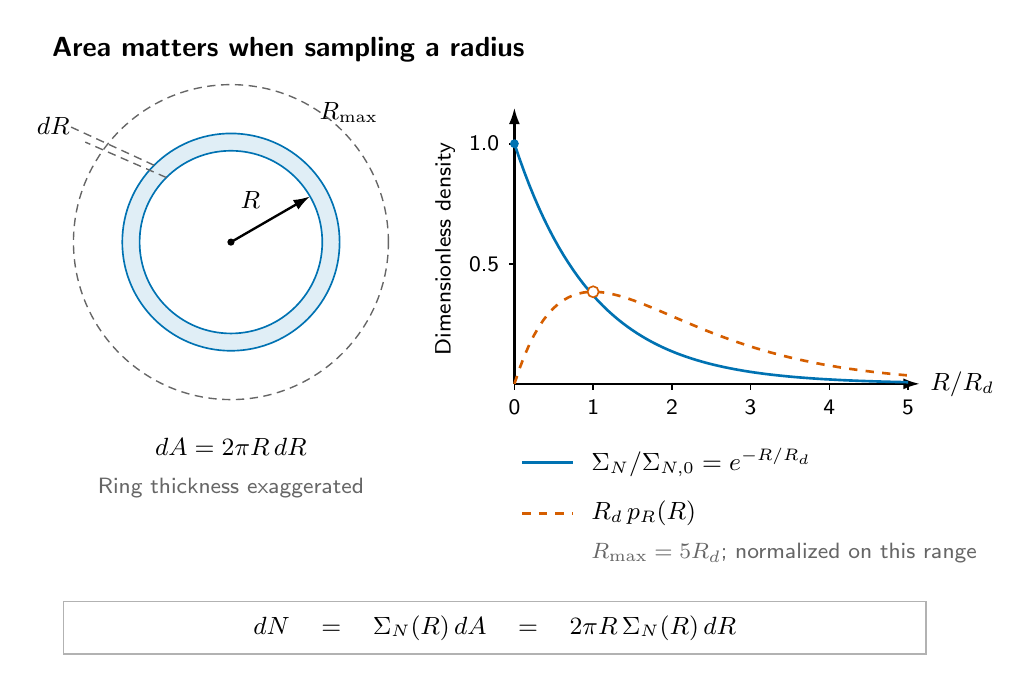
\begin{tikzpicture}[textbook diagram]
  \node[anchor=west,font=\sffamily\bfseries] at (0,4.9) {Area matters when sampling a radius};
  \coordinate (O) at (2.4,2.45);
  \draw[guide] (O) circle (2.0);
  \path[fill=figblue!12,even odd rule] (O) circle (1.38) (O) circle (1.16);
  \draw[figblue] (O) circle (1.16);
  \draw[figblue] (O) circle (1.38);
  \fill (O) circle (1.3pt);
  \draw[vector] (O) -- ($(O)+(30:1.16)$) node[midway,above left] {$R$};
  \draw[guide] ($(O)+(135:1.16)$) -- (0.55,3.72);
  \draw[guide] ($(O)+(135:1.38)$) -- (0.35,3.92);
  \node[anchor=east] at (0.48,3.93) {$dR$};
  \node[anchor=west] at (3.4,4.10) {$R_{\max}$};
  \node at (2.4,-0.15) {$dA=2\pi R\,dR$};
  \node[small label,text=figgray] at (2.4,-0.67) {Ring thickness exaggerated};
  \begin{scope}[shift={(6.0,0.65)},x=1cm,y=3.05cm]
    \draw[vector] (0,0) -- (5.15,0) node[right] {$R/R_d$};
    \draw[vector] (0,0) -- (0,1.15);
    \node[rotate=90,small label] at (-0.88,0.56) {Dimensionless density};
    \foreach \x in {0,1,2,3,4,5} {\draw (\x,0) -- (\x,-0.027); \node[below,small label] at (\x,-0.027) {\x};}
    \foreach \yy in {0.5,1.0} {\draw (0,\yy) -- (-0.065,\yy); \node[left,small label] at (-0.065,\yy) {\yy};}
    \draw[figblue,line width=0.95pt,domain=0:5,samples=81] plot (\x,{exp(-\x)});
    \draw[figred,line width=0.95pt,dashed,domain=0:5,samples=81] plot (\x,{\x*exp(-\x)/(1-6*exp(-5))});
    \fill[figblue] (0,1) circle [radius=1.6pt];
    \draw[figred,fill=white] (1,{exp(-1)/(1-6*exp(-5))}) circle [radius=2pt];
  \end{scope}
  \draw[figblue,line width=0.95pt] (6.10,-0.35) -- (6.75,-0.35);
  \node[anchor=west] at (6.85,-0.35) {$\Sigma_N/\Sigma_{N,0}=e^{-R/R_d}$};
  \draw[figred,line width=0.95pt,dashed] (6.10,-1.00) -- (6.75,-1.00);
  \node[anchor=west] at (6.85,-1.00) {$R_d\,p_R(R)$};
  \node[small label,anchor=west,text=figgray] at (6.85,-1.50) {$R_{\max}=5R_d$; normalized on this range};
  \node[draw=black!30,fill=white,align=center,text width=106mm,inner sep=5pt] at (5.75,-2.45) {$dN=\Sigma_N(R)\,dA=2\pi R\,\Sigma_N(R)\,dR$};
\end{tikzpicture}

\caption{円環の面積と半径の確率密度の関係。面密度に$2\pi R$を掛けて半径の分布へ直します。右側は$R_{\max}=5R_d$で規格化した解析的な入力分布で、標本化した粒子の結果ではありません。面密度は中心で最大でも、半径の確率密度は中心で0です。}
\label{fig:concept-ch4-annulus}
\end{figure}
\FloatBarrier
% END TikZ addition: ch04_annulus

\begin{failbox}{半径を指数乱数にすればよい、とは限りません}
$p_R\propto\exp(-R/R_d)$としてしまうと、円環の面積に由来する$R$を落としてしまいます。また、$R$を一様乱数で選んでも、面積当たり一様な円盤にはなりません。何に対する密度を指定しているかを、最初に確認します。
\end{failbox}

\section{台形則で累積分布関数を作る}
\label{sec:ch4-cdf}
\subsection{半径以内に入る確率を求める}
半径$R$以内に入る確率を、累積分布関数（cumulative distribution function; CDF）と呼びます。ここでは
\begin{equation}
F(R)=\int_0^R p_R(R')\,dR'
=\frac{\displaystyle\int_0^R R'\exp(-R'/R_d)\,dR'}
       {\displaystyle\int_0^{R_{\max}}R'\exp(-R'/R_d)\,dR'}
\label{eq:ch4-cdf-definition}
\end{equation}
です。$F(0)=0$、$F(R_{\max})=1$で、その間で単調に増えます。累積分布とその逆関数から目的の分布に従う乱数を作る考え方は、文献\cite{irifuji1985}の第23章で扱われています。

解析的な比較値も用意できます。$x=R/R_d$、$x_{\max}=R_{\max}/R_d$として
\begin{equation}
C(x)\equiv 1-(1+x)e^{-x}
\label{eq:ch4-C}
\end{equation}
と置きます。$R'\exp(-R'/R_d)$を積分すると$R_d^2 C(R/R_d)$になるので、
\begin{equation}
F(R)=\frac{C(R/R_d)}{C(x_{\max})},\qquad
p_R(R)=\frac{R\exp(-R/R_d)}{R_d^2 C(x_{\max})}
\label{eq:ch4-cdf-exact}
\end{equation}
です。初期分布の規格化定数は$\Sigma_{N,0}=N/[2\pi R_d^2C(x_{\max})]$です。この式は本章の面密度を積分して得た比較用の式であり、数値CDFを作る処理には使いません。

$x_{\max}=5$では$C(x_{\max})=\chfourvalCq$です。無限に延ばした同じ指数分布のうち、約4.04\%が$5R_d$より外側にあります。本章ではそこを初期配置の対象から外し、内側の条件付き分布を確率1へ規格化します。Plummer球の$5a$以内の質量割合とは別の数です。

\subsection{前章の累積積分を再利用する}
分点を$R_j$、被積分関数を$g_j=R_j\exp(-R_j/R_d)$として、台形の面積を順に足します。
\begin{align}
I_0&=0, & I_{j+1}&=I_j+\frac{g_j+g_{j+1}}{2}(R_{j+1}-R_j),\label{eq:ch4-cumulative-trapezoid}\\
\widehat F_j&=\frac{I_j}{I_{N_R}}.\label{eq:ch4-numeric-cdf}
\end{align}
$N_R$は区間数で、分点数は$N_R+1$です。ハットは数値近似を表します。$I_j$の単位は長さの2乗ですが、最後の値で割った$\widehat F_j$は無次元です。

第3章では、有限範囲の累積質量を無条件に全質量$M$へそろえませんでした。ここで最後の値で割ってよいのは、式\eqref{eq:ch4-cdf-definition}そのものが\emph{有限範囲で規格化した確率}だからです。表を都合よく補正する操作ではありません。

\inputcode{chap04/trapezoid}

\subsection{標準条件でCDF表を実装する}
内部単位はkpc、Gyr、$\Msun$です。速度は内部ではkpc\,Gyr$^{-1}$を使い、表示するときだけkm\,s$^{-1}$へ換算します。質量・Plummerスケール長は第3章と共通です。その他の条件は、この章の孤立円盤を確認するために設定しました。
\inputcode{chap04/parameters}

\begin{table}[htbp]
\centering\small
\caption{第4章の標準条件。$N_R$、$N$、$N_{\rm step}$はそれぞれ別の個数です。$R_{\max}$はPlummer球の外縁ではありません。}
\label{tab:ch4-parameters}
\begin{tabular}{ll}\toprule
量 & 設定 \\\midrule
Plummer球 & $M=10^{11}\Msun$, $a=3\unit{kpc}$ \\
粒子の初期分布 & $R_d=3\unit{kpc}$, $R_{\max}=15\unit{kpc}=5R_d$ \\
粒子数・乱数seed & $N=1000$, seed $=42$ \\
CDFの区間数・分点数 & $N_R=4096$, $4097$分点 \\
回転方向 & $s_{\rm rot}=+1$（反時計回り） \\
終時刻・ステップ数 & $t_{\rm end}=0.60\unit{Gyr}$, $N_{\rm step}=3000$ \\
時間刻み・保存間隔 & $\Delta t=0.2\unit{Myr}$、10ステップごと \\\bottomrule
\end{tabular}
\end{table}

\inputcode{chap04/build-cdf}

\texttt{check\_positive}と\texttt{check\_integer}は、正で有限な値、正の整数であることを確認する補助関数です。完全なコードはNotebookに含めます。\texttt{cdf}を後で逆変換するため、隣接する値がすべて増えていることも確認します。標準条件では、$R=0$の被積分関数が0でも最初の台形の面積は正なので、CDFの最初の区間も増えます。

\begin{figure}[htbp]
\centering\includegraphics[width=0.73\linewidth]{\figpath{ch04_cdf}}
\caption{初期円盤のCDF。灰色破線は式\eqref{eq:ch4-cdf-exact}、青実線は台形則による数値表です。有限の初期配置範囲$[0,5R_d]$で規格化しています。}
\label{fig:ch4-cdf}
\end{figure}
分点上で解析式と比較した最大差は$\chfourvalNodeError$でした。図\ref{fig:ch4-cdf}ではほぼ重なりますが、この近似誤差が0という意味ではありません。

\section{線形補間で分点間の値を求める}
\label{sec:ch4-interpolation}
\subsection{2点間の関数を直線で近似する}
CDF表は、決めた分点の値しか持ちません。分点の間の値を求めるため、二つの点を結ぶ直線で近似します。この操作が線形補間です。前章の台形則では同じ直線の下の面積を求めましたが、ここでは直線上の値そのものを使います。

一般の表$(x_j,y_j)$について、$x_j\le x\le x_{j+1}$の位置を
\begin{equation}
\lambda=\frac{x-x_j}{x_{j+1}-x_j}
\label{eq:ch4-fraction}
\end{equation}
で表します。左端なら$\lambda=0$、右端なら$\lambda=1$です。二つの値をその割合で混ぜると、
\begin{equation}
y_{\rm lin}(x)=(1-\lambda)y_j+\lambda y_{j+1}
\label{eq:ch4-linear-interpolation}
\end{equation}
となります。分点では表の値に一致し、その間では両端の値の間を取ります。傾きを用いた$y_j+(y_{j+1}-y_j)(x-x_j)/(x_{j+1}-x_j)$とも同じ式です。補間と補間誤差の一般的な考え方は文献\cite{sugiura2009}の\S2.3を参照してください。

\subsection{一つの点を実装して確かめる}
まず区間を順に探す、短い実装を作ります。区間が見つかったら、式\eqref{eq:ch4-fraction}と式\eqref{eq:ch4-linear-interpolation}を計算するだけです。入力する分点は狭義単調増加とします。
\inputcode{chap04/linear-interpolation}
この関数は表の外では停止します。補間は表の内側での近似であり、外側へ直線を延ばす外挿とは区別します。\texttt{check\_grid}は第3章と同じく、分点・値の配列の形と有限性、分点の増加を確かめます。

多数の点を補間するときには、\texttt{np.interp(x, xp, fp)}を使います。\texttt{xp}が入力側の分点、\texttt{fp}がその値です。自作関数で原理を確認したうえで、同じ区分的な線形補間を行うライブラリ関数に置き換えます。\cite{numpy}全粒子についてPythonで表を繰り返し走査する必要はありません。

\begin{failbox}{増加していない表をそのまま渡さない}
入力側の分点に重複があると、式\eqref{eq:ch4-fraction}の分母が0になります。表を作る段階で、分点が有限で狭義単調増加かを確認します。また、\texttt{np.interp}は既定では表の外で端の値を返します。本章の自作関数とはこの扱いが違うので、呼び出し前に補間点が表の範囲内にあることを確認します。
\end{failbox}

\subsection{線形補間の精度と表の誤差を区別する}
真の関数$f$が滑らかで、両端の値が正しく与えられている場合、線形補間の誤差は区間内のある点$\xi$を使って
\begin{equation}
f(x)-f_{\rm lin}(x)=\frac{f''(\xi)}{2}(x-x_j)(x-x_{j+1})
\label{eq:ch4-interpolation-error}
\end{equation}
と書けます。区間幅を$h$とし、$|f''|$が上から抑えられるなら、誤差の大きさは$\max|f''|\,h^2/8$以下です。これが、滑らかな関数を細かい表で線形補間したとき、通常は幅の2乗で誤差が減る理由です。式は多項式補間の誤差公式の2分点の場合です。\cite{sugiura2009}

ただし、これから使うCDF表の値には台形則の誤差もあります。補間してもその誤差は消えません。さらに、CDFの逆関数は中心近くで傾きが大きくなるため、半径の誤差が全域で単純な同じ比例関係に従うとは限りません。本章では解析CDFに戻した確率のずれを、まず確認します。

\begin{notebox}{ほかの補間法}
多項式補間や三次スプラインは、より多くの分点を使って関数を近似します。高次の方法が有利な場合もありますが、点の間で振動したり、単調性を失ったりしないか確認が必要です。PCHIPは単調性を保つ区分的三次補間の代表例です。\cite{scipy_pchip}本章では、増加する表を扱いやすく実装も短い線形補間に集中します。詳細な理論と代替法の実装は数値計算の教科書に譲ります。
\end{notebox}

\section{一様乱数を円盤の半径へ変換する}
\label{sec:ch4-sampling}
\subsection{CDFの逆向きに表を読む}
$0\le u<1$の一様乱数を一つ選び、$F(R)=u$となる半径を求めます。CDFは「半径から確率」を返しますが、ここでは「確率から半径」を求めます。この方法を逆変換サンプリングと呼びます。\cite{irifuji1985}

なぜこれで正しい分布になるのでしょうか。単調増加する$F$では、生成半径が$R_*$以下になることと、一様乱数が$F(R_*)$以下になることが同値です。一様乱数がその範囲へ入る確率は$F(R_*)$です。このため、生成半径の累積分布は目標の$F$になります。実装では、これを数値表の逆補間で近似します。

$\widehat F_j\le u\le\widehat F_{j+1}$なら、入力側を$\widehat F$、出力側を$R$として
\begin{equation}
\widehat R(u)=R_j+
\frac{u-\widehat F_j}{\widehat F_{j+1}-\widehat F_j}(R_{j+1}-R_j)
\label{eq:ch4-inverse-interpolation}
\end{equation}
です。$\widehat F_j$が増えているので、$\widehat R$は必ず二つの分点の間に入ります。
\inputcode{chap04/inverse-example}
標準表で$u=0.5$を逆変換すると、半径は$\chfourvalHalfInterp\unit{kpc}$でした。自作関数と\texttt{np.interp}の値が一致することを確認します。これは初期円盤の\emph{粒子数}の半分を含む半径で、Plummer球の半質量半径ではありません。

図\ref{fig:ch4-interpolation}の矢印を、縦軸の確率から横軸の半径へたどってください。

\begin{figure}[htbp]
\centering% The original numerical line and analytic CDF are embedded unchanged.
\begin{tikzpicture}[textbook diagram]
  \node[inner sep=0,anchor=south west] (plot) at (0,0) {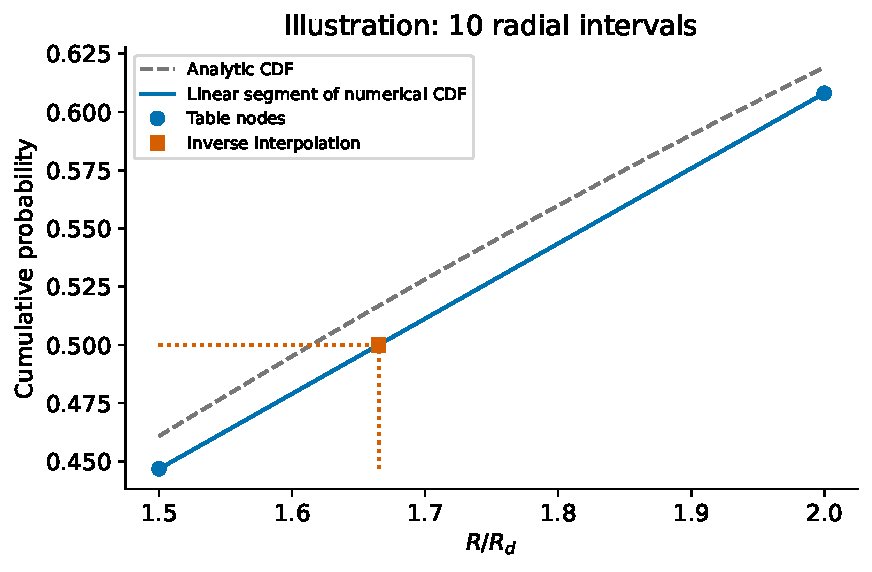
\includegraphics[width=118mm]{figures/ch04_interpolation.pdf}};
  \begin{scope}[x={(plot.south east)},y={(plot.north west)}]
    \draw[vector,figred] (.147,.396700) -- (.422,.396700);
    \draw[vector,figred] (.433970,.380) -- (.433970,.146);
    \node[small label,fill=white,inner sep=1pt,above] at (.245,.402) {$u=0.5$};
    \node[small label,fill=white,inner sep=1pt,anchor=west] at (.453,.196) {$\widehat R(u)/R_d$};
    \node[small label,fill=white,inner sep=1.5pt,anchor=west] (lo) at (.24,.198) {$(R_j,\widehat F_j)$};
    \draw[guide] (lo.west) -- (.182204,.180028);
    \node[small label,fill=white,inner sep=1.5pt,anchor=east] (hi) at (.905,.545) {$(R_{j+1},\widehat F_{j+1})$};
    \draw[guide] (hi.east) -- (.944684,.836223);
  \end{scope}
\end{tikzpicture}

\caption{数値CDFの一つの線分を逆向きに読む例。説明用に10区間だけで作った粗い表を使っています。丸が分点、四角が$u=0.5$の逆補間です。灰色破線の解析CDFとの差も示しています。標準の4096区間の結果とは区別してください。朱色の矢印は$u$から線分へ、そこから$\widehat R(u)$へ読む順序です。表の組$(R_j,\widehat F_j)$を示し、横軸では$R$を$R_d$で規格化しています。}
\label{fig:ch4-interpolation}
\end{figure}

\subsection{乱数を使う前に、逆変換を検証する}
同じ数値表で$u\to\widehat R\to\widehat F$と戻せば、線形補間の範囲ではもとの$u$にほぼ戻ります。しかし、それだけでは数値表が正しいかは分かりません。比較には、独立な解析CDFである式\eqref{eq:ch4-cdf-exact}を使います。

まず分点上の誤差$e_{F,\rm node}$を、次に固定した確率の集合$\mathcal U$上の逆変換の誤差$e_u$を
\begin{align}
e_{F,\rm node}&=\max_j|\widehat F_j-F(R_j)|,\label{eq:ch4-node-error}\\
e_u&=\max_{u\in\mathcal U}|F(\widehat R(u))-u|\label{eq:ch4-inverse-error}
\end{align}
で定義します。本章の$\mathcal U$は0から1までの20001個の等間隔の点です。まだ乱数は使いません。$e_u$は選んだ試験点上の最大値であって、連続な全確率範囲の最大誤差を厳密に保証する値ではありません。
\inputcode{chap04/cdf-convergence}

\begin{table}[htbp]
\centering\small
\caption{CDFの分割数試験。範囲$[0,5R_d]$と試験確率は固定しています。$p_u$は隣接する行の$e_u$の比から求めた推定次数です。}
\label{tab:ch4-cdf-convergence}
\begin{tabular}{rrrrr}\toprule
$N_R$ & $\Delta R\ [\mathrm{kpc}]$ & $e_{F,\rm node}$ & $e_u$ & $p_u$ \\
\midrule
32 & 0.468750 & $1.52\times 10^{-3}$ & $2.45\times 10^{-3}$ & --- \\
64 & 0.234375 & $3.80\times 10^{-4}$ & $6.98\times 10^{-4}$ & 1.8117 \\
128 & 0.117188 & $9.51\times 10^{-5}$ & $1.85\times 10^{-4}$ & 1.9121 \\
256 & 0.058594 & $2.38\times 10^{-5}$ & $4.80\times 10^{-5}$ & 1.9486 \\
512 & 0.029297 & $5.94\times 10^{-6}$ & $1.12\times 10^{-5}$ & 2.0986 \\
\bottomrule\end{tabular}

\end{table}
\begin{figure}[htbp]
\centering\includegraphics[width=0.72\linewidth]{\figpath{ch04_cdf_convergence}}
\caption{数値CDFと逆補間による確率のずれ。点線は最も細かい分割の値を通る傾き2の参照線で、当てはめではありません。試験確率が有限個なので、最大誤差の位置の拾い方も推定次数に影響します。}
\label{fig:ch4-cdf-convergence}
\end{figure}

表\ref{tab:ch4-cdf-convergence}では、分割を細かくすると誤差が減っています。標準の4096区間での$e_u$は$\chfourvalInverseError$でした。この数値誤差と、次に見る有限粒子数のばらつきを分けて考えます。表を細かくするだけで、乱数で配置した点が完全になめらかな分布になるわけではありません。

\subsection{半径と方位角に乱数を与える}
半径のための$u_i$とは別に、一様乱数$w_i$を使って$\phi_i=2\pi w_i$とします。ここで$\phi$は方位角です。二つを独立に選ぶことで、半径によらず方位角を一様にできます。位置は
\begin{equation}
x_i=R_i\cos\phi_i,\qquad y_i=R_i\sin\phi_i
\label{eq:ch4-polar-position}
\end{equation}
です。同じ乱数一つを半径と角度に流用すると両者が関連し、意図した軸対称の分布を作れません。

Notebookでは\texttt{rng = np.random.default\_rng(seed)}で乱数生成器を用意します。\texttt{rng.random((N, 2))}の各行に、半径と角度に使う二つの一様乱数を入れます。seedは実験を再現するための設定です。同じ実装・乱数生成環境・呼び出し順序なら同じ初期値を再現できますが、seedだけで異なる実装や将来のライブラリ環境まで同一の乱数列になると保証はしません。\cite{numpy}配布物には初期配列と使用したNumPyの版も記録します。

\begin{notebox}{ほかの標本化法}
棄却法は、候補の乱数を生成し、目標分布に応じて採用するかを選ぶ方法です。逆関数を求めにくい場合にも使えます。本書では、既習の台形則と今回の補間を一つの計算へ結び付けるため、CDFの逆変換を使います。乱数による積分を含むMonte Carlo法の一般論は、文献\cite{irifuji1985}に譲ります。
\end{notebox}

\section{円運動速度を与えて円盤を作る}
\label{sec:ch4-initial}
\subsection{同じ重力場から初期速度を求める}
粒子を置くだけでは、円盤を回転させたことにはなりません。各半径でPlummer球の円運動速度を与えます。第3章の式を再利用すると、
\begin{equation}
v_c^2(R)=\frac{GMR^2}{(R^2+a^2)^{3/2}}
\label{eq:ch4-circular-speed}
\end{equation}
です。粒子の分布のスケール長$R_d$を、この分母の$a$へ取り違えないようにします。位置の確率を決める式と、重力を決める式は別です。

反時計回りの接線方向の単位ベクトルは$(-\sin\phi,\cos\phi)$です。回転方向を$s_{\rm rot}=+1$または$-1$として、
\begin{equation}
v_{x,i}=-s_{\rm rot} v_c(R_i)\sin\phi_i,\qquad
v_{y,i}=s_{\rm rot} v_c(R_i)\cos\phi_i
\label{eq:ch4-circular-velocity}
\end{equation}
と置きます。例えば正の$x$軸上の粒子は、$s_{\rm rot}=+1$なら正の$y$方向へ動き始めます。すべての粒子に同じ\emph{速度の大きさ}を与えるのではなく、それぞれの$R_i$に対応する$v_c$を使います。

本章の孤立円盤には、もう一つの銀河の軌道はありません。そのため、ここでは反時計回り・時計回りと呼びます。遭遇軌道の向きとの関係で定義するprograde・retrogradeは、第5・6章で扱います。

\inputcode{chap04/plummer-speed}
\subsection{位置と速度を一つの初期配列へまとめる}
半径の標本化、方位角、接線速度を一つの関数にまとめます。位置と速度はそれぞれ形$(N,2)$です。最後に横に並べ、各行に$[x,y,v_x,v_y]$を持つ形$(N,4)$の状態配列を返します。
\inputcode{chap04/make-disk}

標準例では、\texttt{rng = np.random.default\_rng(seed)}を用意して\texttt{make\_disk}に渡します。乱数生成器を関数の中で毎回同じseedへ戻しません。比較実験でまったく同じ初期標本を使う場合だけ、同じseedの生成器を改めて作ります。初期粒子の半径は、今回の標本では約$\chfourvalMinRadius$から$\chfourvalMaxRadius\unit{kpc}$でした。上限15 kpc以内であることを確認します。

\begin{figure}[htbp]
\centering\includegraphics[width=0.65\linewidth]{\figpath{ch04_disk_initial}}
\caption{標準の初期円盤。初期半径による3群を色とマーカーで分けました。この分類は後の時刻でも固定します。中心の黒い十字はPlummerポテンシャルの中心で、追加の質点ではありません。}
\label{fig:ch4-initial}
\end{figure}

\subsection{標本の重心を無条件に原点へ戻さない}
有限個の粒子を乱数で置けば、単純な平均位置が原点に厳密には一致しないことがあります。しかし、ここで重要なのは、各粒子の位置と速度が\emph{固定したPlummer中心に対する円軌道}になっていることです。

粒子の平均位置だけを引くと、各粒子のPlummer中心からの距離が変わります。平均速度だけを引いても、円運動速度との対応が変わります。第2章の有限質量2体系を重心系へ移す操作と混同せず、本章では粒子だけを再中心化しません。原点を移すなら、背景ポテンシャルの中心も含めた座標変換を考える必要があります。

\section{生成した分布を確かめる}
\label{sec:ch4-empirical}
\subsection{累積分布で比べる}
円盤らしく見えることだけでは、式\eqref{eq:ch4-surface-density}に従っているか判断できません。粒子半径を小さい順に並べ、
\begin{equation}
F_N(R)=\frac{1}{N}\sum_{i=1}^N \boldsymbol{1}(R_i\le R)
\label{eq:ch4-empirical-cdf}
\end{equation}
を作ります。$\boldsymbol{1}$は条件が真なら1、偽なら0です。これは、その半径までにある粒子の割合を返す\textbf{経験CDF}です。

有限個の標本なので、$F_N$は幅$1/N$の階段になります。連続的な解析CDFに完全には一致しません。図\ref{fig:ch4-empirical}では、この階段と解析式を比較します。
\begin{figure}[htbp]
\centering\includegraphics[width=0.73\linewidth]{\figpath{ch04_empirical_cdf}}
\caption{1000粒子の経験CDFと目標CDF。数値CDF表の曲線ではなく、実際に生成した粒子から計算した割合です。有限標本のため、解析式の上下にずれます。}
\label{fig:ch4-empirical}
\end{figure}

ずれの指標を$D_N=\sup_R|F_N(R)-F(R)|$とします。並べた半径$R_{(j)}$における階段の直前と直後、つまり$(j-1)/N$と$j/N$を両方比べれば計算できます。
\begin{equation}
D_N=\max_{1\le j\le N}\left\{
\left|\frac{j}{N}-F(R_{(j)})\right|,
\left|\frac{j-1}{N}-F(R_{(j)})\right|
\right\}.
\label{eq:ch4-cdf-distance}
\end{equation}
本章では分布のずれの大きさとして使い、統計的な仮説検定の合否へ直結させません。
\inputcode{chap04/empirical-cdf}
標準標本では$D_N=\chfourvalSampleError$でした。これは数値表の逆変換誤差$\chfourvalInverseError$よりずっと大きい値です。表をさらに細かくしても、この標本のばらつきが同じ割合で減るわけではありません。

\subsection{円環から粒子数面密度を求める}
円環の内側と外側の半径を$R_{j,-},R_{j,+}$とし、その中の粒子数を$N_j$とします。円環の正確な面積を使うと、全粒子数で規格化した数面密度の推定値は
\begin{equation}
\frac{\widehat\Sigma_{N,j}}{N}
=\frac{N_j}{N\pi(R_{j,+}^2-R_{j,-}^2)}
\label{eq:ch4-surface-estimate}
\end{equation}
です。単位はkpc$^{-2}$です。区間の幅だけで割った半径のヒストグラムとは違います。
\inputcode{chap04/surface-profile}

比較する解析値も、円環の中点の値だけでなく、同じ円環の平均
\begin{equation}
\left\langle\frac{\Sigma_N}{N}\right\rangle_j
=\frac{F(R_{j,+})-F(R_{j,-})}{\pi(R_{j,+}^2-R_{j,-}^2)}
\label{eq:ch4-surface-exact-bin}
\end{equation}
を使います。幅の広い円環では、点での値と平均値が異なるためです。時間発展後に、この同じ測り方で初期分布との比較も行います。

\subsection{粒子数とseedを変える}
CDF表を固定したまま、$N=250,1000,4000$で標本化します。各$N$についてseedを42から49まで変え、8回の$D_N$を比較した結果が表\ref{tab:ch4-sampling}です。これは同じ物理モデルを、異なる有限標本で表した比較です。
\begin{table}[htbp]
\centering\small
\caption{粒子数とseedによる経験CDFのずれ。平均・最小・最大は8個のseedでの値です。数値積分法の収束次数を測った表ではありません。}
\label{tab:ch4-sampling}
\begin{tabular}{rrrrr}\toprule
$N$ & $D_N$ (seed 42) & 平均 & 最小 & 最大 \\
\midrule
250 & 0.063392 & 0.052060 & 0.031292 & 0.066533 \\
1000 & 0.029414 & 0.032565 & 0.017673 & 0.055907 \\
4000 & 0.009382 & 0.012820 & 0.007856 & 0.018457 \\
\bottomrule\end{tabular}

\end{table}

粒子数を増やすと、一般には分布のばらつきが小さくなります。ただし、個々のseedについて$D_N$が必ず単調に減るとは限りません。ある領域に入る確率を$p$とすれば、独立な$N$標本による粒子数の分散は$Np(1-p)$です。割合のばらつきの尺度が$N^{-1/2}$になることからも、粒子数と表の刻みは別の役割だと分かります。これは一つの領域の粒子割合に関する見積もりで、表の各$D_N$が厳密に同じ係数で変わるという意味ではありません。

\section{1粒子の式を多数粒子へ拡張する}
\label{sec:ch4-vectorization}
\subsection{まず粒子ごとに計算する}
Plummer球の加速度は、第3章と同じ
\begin{equation}
\avec_i=-\frac{GM\rvec_i}{(R_i^2+a^2)^{3/2}}
\label{eq:ch4-acceleration}
\end{equation}
です。新しいのは粒子番号$i$が1個から$N$個へ増える点だけです。1粒子の成分計算を、まずループに入れます。
\inputcode{chap04/acceleration-loop}

\subsection{配列の軸を明示してまとめる}
\texttt{pos}の形は$(N,2)$です。\texttt{np.sum(pos**2, axis=1)}は各粒子の$x_i^2+y_i^2$を返すので、\texttt{r2}の形は$(N,)$になります。この分母を\texttt{[:, None]}で$(N,1)$へ変形し、各行の$x,y$成分に同じ分母を使います。
\inputcode{chap04/acceleration-vector}

\texttt{axis=0}で足すと、全粒子の$x^2$の和と$y^2$の和になり、別の量です。形が実行可能でも、意図した物理量になっているか確認します。独立なループ版との比較では、今回の差を$GM/a^2$で規格化した最大値は$\chfourvalVectorDiff$でした。演算の並べ方で末尾の桁が変わることはありますが、同じ加速度を計算しています。

この関数は$N\times N$の距離表を作りません。背景の重力を粒子ごとに一度ずつ評価するため、1回の加速度計算に必要な演算量は$N$に比例します。粒子対の重力を足す直接N体計算の$O(N^2)$とは異なります。

\begin{failbox}{粒子番号と座標成分の軸を取り違えない}
位置配列$(N,2)$の第1軸は粒子、第2軸は成分です。\texttt{r2}は各粒子に一つの値を持ちます。分母を$(N,1)$にする操作は、同じ粒子の2成分へ値を対応させるためであり、粒子間相互作用を作る処理ではありません。
\end{failbox}

\section{KDKで円盤を時間発展させる}
\label{sec:ch4-integration}
\subsection{積分器の計算は変えない}
前章のKDK関数は、位置と速度の配列へ加算・乗算する形でした。$(1,2)$を$(N,2)$へ増やしても、更新の4行は変わりません。
\inputcode{chap04/leapfrog-step}

全粒子の最初の半kick、全粒子のdrift、新しい位置での加速度評価、最後の半kickを順に行います。加速度を返し、次のステップへ再利用することも同じです。速度は最後のkickを終えた整数時刻の値を保存します。

\subsection{時間刻みと出力間隔を分ける}
多数粒子の位置と速度を毎ステップすべて保存すると、履歴のメモリが大きくなります。本章では時間積分は3000ステップすべて行いますが、履歴は10ステップごとに保存します。最後の時刻が保存間隔に乗らない場合も、最終状態は必ず保存します。

保存時刻の個数を$N_{\rm save}$とすると、履歴の形は$(N_{\rm save},N,4)$です。\texttt{float64}の各要素を8 byteとして、必要な領域は
\begin{equation}
B=8\times 4\times N\times N_{\rm save}\quad\mathrm{byte}
\label{eq:ch4-memory}
\end{equation}
です。これは履歴配列だけの大きさで、一時配列やNotebookの画像のメモリは含みません。
\begin{table}[htbp]
\centering\small
\caption{標準の1000粒子・3000ステップでの履歴配列。MBは$10^6$ byteです。どちらも時間積分の力評価回数は3001回です。}
\label{tab:ch4-memory}
\begin{tabular}{lrr}\toprule
保存方法 & $N_{\rm save}$ & 履歴の容量 [MB] \\\midrule
毎ステップ & 3001 & $\chfourvalAllMemory$ \\
10ステップごと & 301 & $\chfourvalSavedMemory$ \\\bottomrule
\end{tabular}
\end{table}

\inputcode{chap04/integrate-leapfrog}

\texttt{prepare\_history}は初期値の形$(N,4)$、有限性、正のステップ数などを確認し、保存するステップ番号と配列を用意します。詳しいコードはNotebookに置きます。ループは保存の有無と無関係に毎ステップ進みます。標準の時間刻みは0.2 Myr、保存間隔は2 Myrです。\texttt{history[j]}の$j$は保存番号であり、積分した全ステップの番号ではありません。

\subsection{孤立円盤を0.6 Gyr進める}
初期配列を作った後、\texttt{integrate\_leapfrog}へ加速度関数、終時刻、ステップ数、$M,a$を渡します。標準では初回の加速度と3000回の更新で、合計3001回の加速度関数の呼び出しです。各呼び出しで1000粒子分をまとめて評価します。

中心近くの角速度は$\Omega_0=\sqrt{GM/a^3}$に近づきます。対応する周期は$2\pi\sqrt{a^3/(GM)}\simeq\chfourvalCorePeriod\unit{Myr}$です。円盤全体で一つの周期があるわけではありません。中心側の短い時間尺度も意識して刻みを選び、後の刻み試験で確認します。

\begin{figure}[htbp]
\centering\includegraphics[width=0.65\linewidth]{\figpath{ch04_disk_final}}
\caption{0.60 Gyr後の孤立円盤。軸範囲、初期半径による色・マーカー分類は図\ref{fig:ch4-initial}と同じです。各粒子の方位角は変わっていますが、半径方向の分布はほぼ保たれています。}
\label{fig:ch4-final}
\end{figure}

円運動の初期条件では、連続的な軸対称の数面密度は時間に依存しません。ただし、角速度は半径によって異なるので、有限個の点の模様全体が一枚の板のように剛体回転するわけではありません。\emph{密度分布が定常であること}と、\emph{個々の粒子が動かないこと}は別です。

\section{分布の維持と軌道の精度を確認する}
\label{sec:ch4-validation}
\subsection{初期と終時刻の数面密度を比較する}
初期と終時刻に同じ円環を用い、式\eqref{eq:ch4-surface-estimate}で数面密度を測ります。図\ref{fig:ch4-profile}の灰色点線は、式\eqref{eq:ch4-surface-exact-bin}の円環平均です。初期標本からのばらつきが、時間積分中に新しく生じた数値誤差であるとは限りません。
\begin{figure}[htbp]
\centering\includegraphics[width=0.74\linewidth]{\figpath{ch04_surface_profile}}
\caption{円環で測った数面密度。青丸が初期、朱色の白抜き四角が終時刻です。縦軸は$R_d^2\widehat\Sigma_N/N$です。粒子数の少ない外側では標本のばらつきが目立ちますが、初期と終時刻の曲線はほぼ重なります。}
\label{fig:ch4-profile}
\end{figure}

経験CDFのずれは、初期で$\chfourvalSampleError$、終時刻で$\chfourvalFinalCDF$でした。小さな違いはあっても、有限粒子数に由来する初期のずれが支配的です。ここで確かめているのは、固定ポテンシャル中の円軌道の集合が保たれることです。自己重力円盤の集団的な安定性を調べた結果とは解釈しません。

\subsection{各粒子の保存量を計算する}
固定した球対称場なので、各粒子の比エネルギーと比角運動量を使います。
\begin{equation}
\varepsilon_i=\frac{v_{x,i}^2+v_{y,i}^2}{2}+\Phi(R_i),\qquad
\ell_{z,i}=x_i v_{y,i}-y_i v_{x,i}.
\label{eq:ch4-invariants}
\end{equation}
ここでも粒子の質量を掛けません。Plummer球の全エネルギーや、質量をもつ円盤全体のエネルギーを計算するのではありません。
\inputcode{chap04/diagnostics}

履歴は3軸なので、成分を足す軸は\texttt{axis=2}です。半径・エネルギー・角運動量の返り値は、いずれも$(N_{\rm save},N)$です。全粒子のエネルギー変化を先に足すと、正負の誤差が相殺されることがあるため、粒子ごとの誤差を調べます。

本章の円軌道では全粒子の$\varepsilon_i^0<0$なので、エネルギー誤差は各初期値の絶対値で割れます。一方、中心に近い粒子では$\ell_{z,i}^0$が小さくなります。角運動量には共通の正の尺度$\ell_*=R_dv_c(R_d)$を使い、
\begin{equation}
e_\varepsilon=\max_{n,i}\frac{|\varepsilon_i^n-\varepsilon_i^0|}{|\varepsilon_i^0|},\qquad
e_\ell=\max_{n,i}\frac{|\ell_{z,i}^n-\ell_{z,i}^0|}{\ell_*}
\label{eq:ch4-conservation-errors}
\end{equation}
とします。この$e_\ell$は、各粒子の初期角運動量に対する相対誤差ではありません。

\subsection{初期条件から同時刻の解析位置を作る}
円盤が円く見えることだけでは、回転の速さまで正しいと分かりません。本章では全粒子に円運動を与えたので、初期半径から
\begin{equation}
\Omega_i=\frac{\sqrt{GM}}{(R_i(0)^2+a^2)^{3/4}}
\label{eq:ch4-omega}
\end{equation}
を求められます。解析的な方位角は$\phi_i(t)=\phi_i(0)+s_{\rm rot}\Omega_it$です。この関係で初期位置を回転させ、同じ時刻の数値位置と比較します。比較の途中で数値解の半径から$\Omega_i$を更新してはいけません。
\inputcode{chap04/exact-disk}

式\eqref{eq:ch4-omega}は原点でも有限です。原点にちょうど置いた粒子は初期位置が0なので、この回転式でもそのまま0にとどまります。$v_c/R$をそのまま数値的に評価する場合の$0/0$を作りません。

位置の誤差と半径だけの変化は、別に定義します。
\begin{equation}
e_{\rm pos}=\max_{n,i}\frac{|\rvec_i^n-\rvec_{i,\rm exact}(t_n)|}{R_d},\qquad
e_R=\max_{n,i}\frac{|R_i^n-R_i^0|}{R_d}.
\label{eq:ch4-position-errors}
\end{equation}
すべての粒子に共通の$R_d$で規格化します。$n$は、ここでは検証に使う保存時刻を走る添字です。したがって、これらは保存時刻における最大値であり、保存していない時刻の最大誤差まで保証するものではありません。
\inputcode{chap04/disk-errors}

\begin{table}[htbp]
\centering\small
\caption{標準の1000粒子・0.60 Gyr・3000ステップの確認。301個の保存時刻と全粒子について最大値を取りました。規格化は式\eqref{eq:ch4-conservation-errors}、式\eqref{eq:ch4-position-errors}です。}
\label{tab:ch4-errors}
\begin{tabular}{lr}\toprule
指標 & 値 \\
\midrule
位置 $e_{\rm pos}$ & $5.46\times 10^{-4}$ \\
半径 $e_R$ & $4.73\times 10^{-5}$ \\
比エネルギー $e_\varepsilon$ & $2.19\times 10^{-9}$ \\
比角運動量 $e_\ell$ & $5.00\times 10^{-14}$ \\
\bottomrule\end{tabular}

\end{table}

位置誤差は$\chfourvalPosError$、半径の変化は$\chfourvalRadiusError$でした。比エネルギーの相対誤差は$\chfourvalEnergyError$で、角運動量のずれは$\chfourvalAngularError$です。中心力のkickとdriftが角運動量を保つ性質は、各粒子にそのまま成り立ちます。一方、エネルギー差や位相の差は有限刻みで残ります。表\ref{tab:ch4-errors}は本章の実測値で、任意の円盤・刻みで同じ値になるという主張ではありません。

\section{数値実験の条件を一つずつ変える}
\label{sec:ch4-experiments}
\subsection{時間刻みだけを変える}
初期配列\texttt{state0}を保存し、同じ終時刻0.60 Gyrまで750、1500、3000、6000ステップで進めます。この比較では乱数を引き直しません。また、各計算の保存時刻を151個の同じ時刻にそろえ、式\eqref{eq:ch4-position-errors}を比べます。
\inputcode{chap04/orbit-convergence}

\begin{table}[htbp]
\centering\small
\caption{同じ初期粒子を使ったKDKの時間刻み試験。全行で終時刻と151個の評価時刻をそろえています。$p$は隣接する行の$e_{\rm pos}$から求めた推定次数です。}
\label{tab:ch4-orbit-convergence}
\begin{tabular}{rrrrr}\toprule
$N_{\rm step}$ & $\Delta t\ [\mathrm{Myr}]$ & $e_{\rm pos}$ & $p$ & 力評価回数 \\
\midrule
750 & 0.8000 & $8.74\times 10^{-3}$ & --- & 751 \\
1500 & 0.4000 & $2.18\times 10^{-3}$ & 2.00069 & 1501 \\
3000 & 0.2000 & $5.46\times 10^{-4}$ & 2.00017 & 3001 \\
6000 & 0.1000 & $1.36\times 10^{-4}$ & 2.00004 & 6001 \\
\bottomrule\end{tabular}

\end{table}
\begin{figure}[htbp]
\centering\includegraphics[width=0.73\linewidth]{\figpath{ch04_orbit_convergence}}
\caption{時間刻みと最大位置誤差。点線は最も細かい刻みの点を通る傾き2の参照線です。粒子数やCDF表ではなく、軌道を進める刻みだけを変更しています。}
\label{fig:ch4-orbit-convergence}
\end{figure}

最も細かい側の推定次数は$\chfourvalOrbitOrder$となり、2次精度を確認できます。保存量が良好でも、同じ時刻の位置を独立に確かめることを続けます。円運動速度を変更した非円軌道の実験には、この円軌道の解析位置を使いません。

\subsection{粒子数・CDF表・保存間隔の役割を区別する}
本章には複数の「数」が出てきました。$N_R$を増やすとCDFの積分・逆補間の精度が変わります。$N$を増やすと分布を表す標本が増えます。$N_{\rm step}$を増やすと、同じ終時刻へ進む時間刻みが細かくなります。\texttt{save\_every}を変えると、履歴の容量と、保存された時刻で見つけられる変動が変わります。

保存の頻度だけを変えても、同じ初期値・同じKDK更新なら終点は変わりません。ただし、粗い出力では短い時間の変動や誤差のピークを見逃すことがあります。「図がなめらかになること」と「運動方程式を高精度で解くこと」を混同しないようにします。

\subsection{回転方向を逆にする}
同じ初期半径・方位角で$s_{\rm rot}=-1$にすれば、初期位置は同じ、速度は逆になります。比エネルギーは同じで、角運動量は符号を反転します。固定した球対称場では、どちらの向きでも円軌道を作れます。本章の再計算でも、時計回りの解析位置に対する誤差は$\chfourvalReverseError$でした。

一般の乱数配置について、初期位置をそのままに速度だけを反転しても、円盤のすべての点が同じ時刻に$x$軸の鏡映になるわけではありません。対応するのは同じ初期位置から時間を逆向きにたどる運動です。個々の粒子は動いても、連続的な軸対称分布は両方で同じです。

\subsection{静止画とアニメーションを比較する}
Notebookでは、保存済みの履歴から円盤のアニメーションを作ります。全粒子のうち3個だけを別のマーカーで追い、星が実際に動いていることも見られるようにしています。これらの粒子に特別な質量や力を与えてはいません。

再生間隔は画面表示の速度です。物理的な$\Delta t$とも、履歴の保存間隔とも異なります。動画を見るだけで検証を終えず、初期・終時刻の静止画、数面密度、保存量、位置誤差も残します。

\section{本章のまとめ}
\label{sec:ch4-summary}
本章では、静的なPlummer球の中で回転するテスト粒子円盤を作りました。円盤の数面密度に円環の面積を掛けると、半径の確率密度が得られます。台形則で累積分布関数を作り、線形補間でその逆関係を読み、一様乱数を半径へ変換しました。方位角には独立な乱数を使います。

Plummer球の円運動速度を半径ごとに与え、1粒子の加速度を多数粒子の配列へ拡張しました。KDKの更新式はそのまま再利用し、計算済みの加速度を次のステップへ渡しました。多数粒子を置いても、粒子同士の重力は含めていません。

数値CDFの誤差、有限粒子数のばらつき、軌道積分の誤差は、別の比較で確認しました。円盤の形が保たれることに加えて、各粒子の保存量と、同時刻の解析位置を調べました。出力を間引くことと、時間刻みを大きくすることも区別しました。

第5章では、この円盤を二つ用意します。第2章の銀河中心の運動、第3章のPlummer重力、第4章の円盤初期条件を組み合わせ、互いに接近させます。今回確かめた孤立円盤を基準にすることで、相互作用による変化と、初期条件や数値誤差による変化を区別しやすくなります。

\chapterexercises
\paragraph{演習4.1　確認：面密度と半径の分布}
$R_d=3\unit{kpc}$、$R_{\max}=5R_d$について、$p_R(R)$の規格化を確認してください。$R<R_d$の粒子割合を求め、$N=1000$なら平均的に何個入るか答えてください。$p_R\propto e^{-R/R_d}$とした場合に、何を落としているかも説明してください。

\paragraph{演習4.2　確認：線形補間と逆補間}
表$(x_j,y_j)=(0,0),(1,2),(3,3)$に対して、$x=2$の$y$を自作関数と\texttt{np.interp}で求めてください。次に$y=2.5$に対応する$x$を、表の入力側と出力側を交換して求めてください。$y=4$を渡す場合は、本章の自作関数と\texttt{np.interp}の既定の扱いにどのような違いがありますか。

\paragraph{演習4.3　確認：有限範囲の規格化と中央値}
CDF表の最後の値を1にすることが、第3章のPlummer累積質量を無条件に全質量へそろえることと異なる理由を述べてください。$F(R)=0.5$を数値表の逆補間で解き、解析CDFを既習の二分法で解いた値と比較してください。両者の差と、実際に生成した1000粒子の半径の中央値のずれは、同じ原因でしょうか。

\paragraph{演習4.4　応用：粒子数と乱数seed}
表\ref{tab:ch4-sampling}と同じ$N$、seedで経験CDFのずれを計算してください。$N$を変える実験では、$M,a,R_d,R_{\max},N_R$を固定します。粒子数を増やしても1粒子の軌道計算の次数が上がるわけではない理由を説明してください。

\paragraph{演習4.5　応用：時間刻みと保存間隔}
まず同じ初期配列で時間刻みを変え、KDKの2次精度を確認してください。次に時間刻みを固定して、\texttt{save\_every=1,10,50}を比べてください。各計算の最終配列、保存時刻数、履歴の容量はどうなりますか。粗い出力で求めた最大誤差を、全ステップの最大誤差と呼べるでしょうか。

\paragraph{演習4.6　応用：回転方向}
同じseed・同じ粒子数で$s_{\rm rot}=+1,-1$の初期条件を作ってください。位置が一致し、速度だけが符号反転すること、初期比エネルギーが一致し、比角運動量の符号が反転することを確認してください。両方をKDKで進め、それぞれに対応する円運動の解析位置と比較してください。

\paragraph{演習4.7　発展：円運動速度の80\%で始める}
初期位置を標準円盤と同じに保ち、初期速度だけを0.8倍してください。半径分布の時間変化と各粒子の保存量を調べてください。この実験を自己重力円盤の不安定性と呼んでよいでしょうか。また、標準の円運動の解析位置との差を、そのまま数値誤差と呼べない理由を説明してください。

\newcommand{\chfivevalVr}{-158.295116}
\newcommand{\chfivevalVt}{59.829889}
\newcommand{\chfivevalSpeed}{169.224583}
\newcommand{\chfivevalPeri}{8.000004531}
\newcommand{\chfivevalTperi}{0.269900}
\newcommand{\chfivevalDt}{0.050}
\newcommand{\chfivevalNstep}{12000}
\newcommand{\chfivevalForce}{12001}
\newcommand{\chfivevalSaveEvery}{40}
\newcommand{\chfivevalHistoryMB}{19.283264}
\newcommand{\chfivevalCenterMB}{0.768064}
\newcommand{\chfivevalEnergyError}{3.30\times 10^{-6}}
\newcommand{\chfivevalAngularError}{5.19\times 10^{-15}}
\newcommand{\chfivevalOuterOne}{0.425}
\newcommand{\chfivevalOuterTwo}{0.432}
\newcommand{\chfivevalLastRatio}{3.97963}
\newcommand{\chfivevalLastDifference}{1.61\times 10^{-2}}
\newcommand{\chfivevalLastDifferenceKpc}{0.048}
\newcommand{\chfivevalLastRMS}{1.68\times 10^{-4}}
\newcommand{\chfivevalWatchRadius}{9.002224}
\newcommand{\chfivevalWatchChange}{0.228686}
\newcommand{\chfivevalBoostDiff}{4.50\times 10^{-10}}
\newcommand{\chfivevalRetroOne}{0.425}
\newcommand{\chfivevalRetroTwo}{0.065}
\newcommand{\chfivevalMemorySeries}{768.832,19.283,3.908}
\newcommand{\chfivevalSavedSeries}{12001,301,61}

\chapter{2つの銀河を接近させる}
\label{chap:interaction}

第4章では、一つの固定したPlummerポテンシャル中に、回転するテスト粒子円盤を作りました。この章では、その円盤を二つ用意して互いに接近させます。第2章の重心と相対運動、第3章のPlummer重力、第4章の円盤生成を組み合わせ、本書の中心となる銀河相互作用の計算を完成させます。

新しい数値積分法は導入しません。時間発展には、引き続き加速度を再利用するKDK leapfrogを使います。今回新しく考えるのは、\textbf{銀河中心も星も動く状況で、どの位置から、どの粒子への重力を計算するか}です。初期状態を作り、中心軌道を確認してから、潮汐テイルやブリッジを見ます。見た目の変化と数値誤差を区別するため、同じ初期粒子を使った時間刻みの比較も行います。

\begin{goalbox}[この章で学ぶこと]
\begin{itemize}
\item 移動するPlummerポテンシャルと、星を表すテスト粒子の役割を区別できます。
\item 採用した中心間ポテンシャルに合わせて、近点距離を指定した初期軌道を作れます。
\item 円盤の局所的な位置・速度を慣性系へ移し、銀河中心と星を同じ時刻へ更新できます。
\item 中心軌道の保存量と、時間に依存する重力場中の粒子のエネルギー変化を区別できます。
\item 潮汐構造を図と粒子割合で調べ、時間刻みによる結果の違いを確認できます。
\end{itemize}
\end{goalbox}

\section{これまでの計算要素を一つにまとめる}
\label{sec:ch5-model}
\subsection{銀河を変形しない重力場として表す}
各銀河$k=1,2$に、一定の全質量$M_k$とPlummerスケール長$a_k$を与えます。銀河中心の位置・速度を$\Rvec_k,\Vvec_k$とし、その中心を動かします。一方、$M_k$と$a_k$自体は時間とともに変えません。したがって、移動するのは\textbf{形を固定した解析的ポテンシャル}です。Plummer球を多数の質量粒子で表し、その変形まで計算するわけではありません。

円盤の星は、質量ゼロのテスト粒子$\rvec_i,\vvec_i$です。星は両銀河の重力を受けますが、星同士の重力や、星から銀河中心への反作用は計算しません。粒子の表示上の重みを、Plummer球の質量と足し合わせることもしません。第4章の粒子数面密度$\Sigma_N$と、重力を作る質量分布の区別を引き継ぎます。

\begin{table}[htbp]
\centering
\caption{本章で計算する重力の関係。「力を受ける側」と「重力を作る側」を区別します。星には出身銀河だけでなく、両銀河の重力を与えます。}
\label{tab:ch5-coupling}
\begin{tabularx}{\linewidth}{lX}
\toprule
力を受ける側 & 計算する重力 \\
\midrule
銀河中心1・2 & 中心間の有効対ポテンシャルから求める相互力 \\
テスト粒子 & 二つの移動するPlummerポテンシャルの重力の和 \\
テスト粒子間 & 計算しません \\
テスト粒子から中心 & 計算しません \\
\bottomrule
\end{tabularx}
\end{table}

外部重力、ガス、星形成、動力学的摩擦は含めません。すべての位置と速度を一つの慣性系で計算し、運動は$x$--$y$平面内に限定します。円盤が変形しても、背景のPlummer球は同じ形です。ここで再現するのは、簡略化した重力モデルに対する星の軌道の応答です。

\subsection{本章で統合する要素を確認する}
第2章の相対位置・相対速度を
\begin{equation}
\Dvec=\Rvec_2-\Rvec_1,\qquad D=|\Dvec|,\qquad \Uvec=\Vvec_2-\Vvec_1
\label{eq:ch5-relative}
\end{equation}
と書きます。銀河中心の軌道を決めた後、第4章の円盤を各中心の周りへ配置します。必要な操作は、重心系の初期軌道、円盤の初期位置・速度、加速度の計算、KDKの時間更新の四つです。

台形則と線形補間は円盤のCDF生成で再利用します。求根法は第3章の半質量半径などを求める道具として既習ですが、\textbf{本章の標準計算では新たな求根を無理に挿入しません}。後述する中心軌道の初期速度は、保存量から直接求められるためです。各手法は、必要な役割を持つ場所で使います。

\section{動いている中心から重力を求める}
\label{sec:ch5-gravity}
\subsection{テスト粒子が受ける二つのPlummer場を合成する}
銀河$k$の中心から星までの相対位置を
\begin{equation}
\boldsymbol s_{k,i}=\rvec_i-\Rvec_k
\label{eq:ch5-local-position}
\end{equation}
とします。第3・4章の原点からの位置を、この相対位置へ置き換えます。銀河$k$によるポテンシャルと加速度は
\begin{align}
\Phi_k(\rvec_i,t)&=-\frac{GM_k}{\sqrt{|\boldsymbol s_{k,i}|^2+a_k^2}},
\label{eq:ch5-moving-potential}\\
\avec_{k,i}&=-GM_k\frac{\boldsymbol s_{k,i}}{(|\boldsymbol s_{k,i}|^2+a_k^2)^{3/2}}
\label{eq:ch5-moving-acceleration}
\end{align}
です。Plummer球の形は固定でも、中心が動くため、慣性系ではポテンシャルが時間に依存します。Plummer場の式そのものは前章と同じです。\cite{bt2008}

まず1粒子の$x$成分だけを見ると、中心位置$X_k$を使って
\begin{equation}
a_{x,k,i}=-\frac{GM_k(x_i-X_k)}{[(x_i-X_k)^2+(y_i-Y_k)^2+a_k^2]^{3/2}}
\label{eq:ch5-component}
\end{equation}
です。原点ではなく、動く銀河中心へ向かう加速度であることを確認してください。前章の配列計算では、最初に\texttt{pos - center}を計算するだけで同じ置き換えができます。
\inputcode{chap05/moving-plummer}

各星の運動方程式は
\begin{equation}
\frac{d\rvec_i}{dt}=\vvec_i,\qquad \frac{d\vvec_i}{dt}=\avec_{1,i}+\avec_{2,i}
\label{eq:ch5-tracer-ode}
\end{equation}
です。どちらの円盤から出発した星も、同じ二つの場の和を受けます。出身銀河の番号は色分けと解析に使うだけで、重力源を選別する番号ではありません。

\subsection{中心間の相互作用を別に定義する}
中心の運動にも、有限の大きさを反映した滑らかな力を使います。本章では二つの中心の有効な対ポテンシャルエネルギーを
\begin{equation}
W_{\rm c}(D)=-\frac{GM_1M_2}{\sqrt{D^2+b^2}}
\label{eq:ch5-pair-potential}
\end{equation}
と\textbf{モデルとして定義}します。$b$は中心間力に使う共通の有効長さです。$a_1,a_2$は星が受ける各Plummer場のスケール長なので、記号を分けます。

式\eqref{eq:ch5-pair-potential}は、\textbf{二つの広がったPlummer密度分布どうしの厳密な相互作用エネルギーではありません}。その計算には、各分布の広がりにわたって相互作用を足す必要があります。本章はその積分を追加せず、中心軌道のための簡単な有効モデルを採用します。後で与える$b=3\unit{kpc}$も、この教材の選択です。

同じ$W_{\rm c}$から両方の力を求めると、中心加速度は
\begin{equation}
\boldsymbol A_1=+GM_2\frac{\Dvec}{(D^2+b^2)^{3/2}},\qquad
\boldsymbol A_2=-GM_1\frac{\Dvec}{(D^2+b^2)^{3/2}}
\label{eq:ch5-center-acceleration}
\end{equation}
になります。この二つは$M_1\boldsymbol A_1+M_2\boldsymbol A_2=0$を満たします。第2章と同じく、共通部分を一度だけ計算します。
\inputcode{chap05/center-acceleration}

$b$は両方の式で同じ値です。$M_1\ne M_2$の場合でも作用・反作用を保ちます。$a_1\ne a_2$へ拡張するとき、中心1へは$a_2$、中心2へは$a_1$をそのまま代入すると、一般に二つの力の大きさが一致しません。その置き換えは行いません。本章の主実験では$a_1=a_2=b$に固定します。

この選択には、力の対応を単純にする利点があります。$b=a_2$なら、中心1への加速度は銀河2のPlummer場を$\boldsymbol R_1$で評価した値に一致します。中心2についても同じ対応を保つため、標準では$b=a_1=a_2$とします。その結果、星と出身中心が受ける相手の重力の差を、同じ場の二つの位置での評価として書けます。ただし、これは本章の有効モデル内での整合性であり、広がった二つの球の厳密な相互力を得たという意味ではありません。


\begin{failbox}{Plummer場と中心間力を同じ意味にしない}
星は式\eqref{eq:ch5-moving-potential}の場を受け、中心は式\eqref{eq:ch5-pair-potential}で動きます。形が似ていても、後者は本章で定義した有効な粒子対のモデルです。有限サイズの銀河を厳密に剛体として相互作用させた計算、と説明しないようにします。
\end{failbox}


% BEGIN TikZ addition: ch05_force_model
図\ref{fig:concept-ch5-forces}に、このモデルで計算する作用をまとめました。中心間の有効長さ$b$と、星が受けるPlummer場の$a_k$を区別し、矢印のない反作用を計算へ加えていないことを確認してください。
\begin{figure}[!htbp]
\centering
% Dependency arrows, not spatial force vectors.
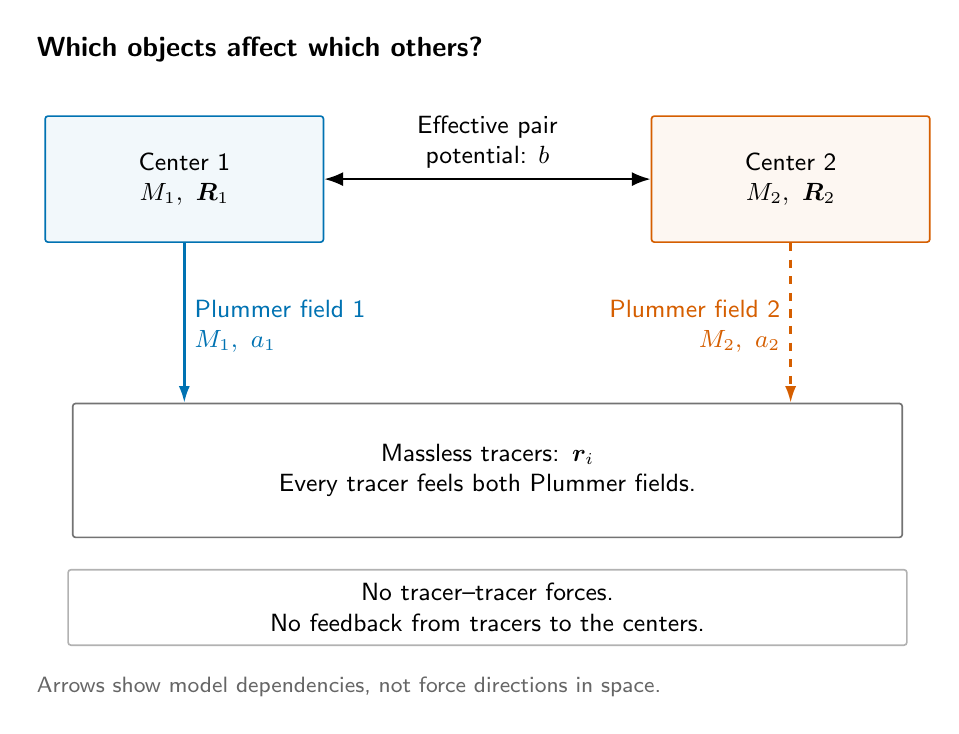
\begin{tikzpicture}[textbook diagram]
  \node[anchor=west,font=\sffamily\bfseries] at (0,4.45) {Which objects affect which others?};
  \node[draw=figblue,fill=figblue!5,rounded corners=1pt,text width=33mm,minimum height=16mm,align=center] (c1) at (2.0,2.80) {Center 1\\$M_1,\ \boldsymbol R_1$};
  \node[draw=figred,fill=figred!5,rounded corners=1pt,text width=33mm,minimum height=16mm,align=center] (c2) at (9.7,2.80) {Center 2\\$M_2,\ \boldsymbol R_2$};
  \draw[{Latex}-{Latex},line width=0.85pt] (c1.east) -- node[above,align=center] {Effective pair\\potential: $b$} (c2.west);
  \node[draw=black!55,fill=white,rounded corners=1pt,text width=103mm,minimum height=17mm,align=center] (stars) at (5.85,-0.90) {Massless tracers: $\boldsymbol r_i$\\Every tracer feels both Plummer fields.};
  \draw[vector,figblue] (c1.south) -- node[right,align=left,pos=.52] {Plummer field 1\\$M_1,\ a_1$} (2.0,-.04);
  \draw[vector,figred,dashed] (c2.south) -- node[left,align=right,pos=.52] {Plummer field 2\\$M_2,\ a_2$} (9.7,-.04);
  \node[draw=black!30,rounded corners=1pt,text width=103mm,align=center,inner sep=5pt] at (5.85,-2.64) {No tracer--tracer forces.\\No feedback from tracers to the centers.};
  \node[small label,text=figgray,anchor=west] at (0,-3.65) {Arrows show model dependencies, not force directions in space.};
\end{tikzpicture}

\caption{中心とテスト粒子の間で計算する作用の関係。横の双方向矢印は共通の有効長さ$b$を使う中心間相互作用、下向き矢印は各Plummer場から星への作用です。星から中心への反作用と星同士の重力は計算しません。矢印はモデルの依存関係であり、空間内の力の向きではありません。}
\label{fig:concept-ch5-forces}
\end{figure}

% END TikZ addition: ch05_force_model

\Needspace{10\baselineskip}
\section{近点距離に合った初期軌道を作る}
\label{sec:ch5-initial-orbit}
\subsection{点質量の速度をそのまま使わない}
銀河中心の相対加速度は、式\eqref{eq:ch5-center-acceleration}の差から
\begin{equation}
\frac{d\Uvec}{dt}=-\frac{\mu\Dvec}{(D^2+b^2)^{3/2}},\qquad \mu=G(M_1+M_2)
\label{eq:ch5-relative-ode}
\end{equation}
です。その相対運動の比エネルギーと比角運動量は
\begin{equation}
\varepsilon=\frac{U^2}{2}-\frac{\mu}{\sqrt{D^2+b^2}},\qquad h=(\Dvec\times\Uvec)_z
\label{eq:ch5-orbital-invariants}
\end{equation}
で、どちらも時間によらず一定になります。第2章の$-\mu/D$とはポテンシャルが異なります。同じ$\mu$と近点距離を選んでも、初期速度は改めて求めます。

本章では$\varepsilon=0$の内向きの遭遇を作ります。これは無限遠をポテンシャルの零点とした、束縛・非束縛の境界のエネルギーです。ただし、$b>0$では力が厳密な逆2乗則ではないため、\textbf{軌道の形をKepler放物線と呼ぶことはできません}。$b\to0$の極限で、第2章の放物線に対応します。

\subsection{近点から角運動量を決める}
初期距離を$D_0$、目標の近点距離を$D_p$とし、$0<D_p<D_0$を選びます。近点では動径速度が0なので、速度の大きさは接線速度$U_p$です。$\varepsilon=0$を使うと
\begin{equation}
U_p^2=\frac{2\mu}{\sqrt{D_p^2+b^2}},\qquad
h^2=D_p^2U_p^2=\frac{2\mu D_p^2}{\sqrt{D_p^2+b^2}}
\label{eq:ch5-pericenter-angular}
\end{equation}
です。ここでは$h>0$を選び、軌道の向きを反時計回りにします。

初期位置を$\Dvec(0)=(D_0,0)$とすれば、角運動量から接線速度$U_t=h/D_0$が決まります。初期位置でも$\varepsilon=0$とし、動径速度の内向きの符号を選ぶと
\begin{equation}
U_t=\frac{h}{D_0},\qquad
U_r=-\sqrt{\frac{2\mu}{\sqrt{D_0^2+b^2}}-U_t^2},\qquad
\Uvec(0)=(U_r,U_t)
\label{eq:ch5-incoming-speed}
\end{equation}
となります。これは採用した有効ポテンシャルから直接求めた初期条件で、近点を数値計算後に合わせ直す操作ではありません。

\subsection{重心系の二つの位置・速度へ変換する}
第2章の重心変換を再利用します。初期重心を原点、重心速度を0とすれば、$\Mtot=M_1+M_2$として
\begin{align}
\Rvec_1(0)&=-\frac{M_2}{\Mtot}\Dvec(0),&
\Rvec_2(0)&=+\frac{M_1}{\Mtot}\Dvec(0),\notag\\
\Vvec_1(0)&=-\frac{M_2}{\Mtot}\Uvec(0),&
\Vvec_2(0)&=+\frac{M_1}{\Mtot}\Uvec(0)
\label{eq:ch5-barycentric-initial}
\end{align}
です。相対距離・相対速度を、それぞれの中心から原点までの距離・速度と取り違えないようにします。
\inputcode{chap05/encounter-initial}

返り値は形$(2,4)$の配列です。各行に銀河中心の$[X_k,Y_k,V_{x,k},V_{y,k}]$を入れます。\texttt{weights}は式\eqref{eq:ch5-barycentric-initial}の二つの係数です。\texttt{[:, None]}で列を加え、各係数を$x,y$の両成分に掛けています。

\section{二つの円盤を配置する}
\label{sec:ch5-disk-initial}
\subsection{円盤の内部運動と銀河全体の運動を分ける}
各円盤の粒子数面密度は、第4章と同じ切断指数分布です。
\begin{equation}
\Sigma_{N,k}(R)\propto e^{-R/R_{d,k}},\qquad 0\le R\le R_{\max,k}.
\label{eq:ch5-disk-profile}
\end{equation}
この$R$は各銀河中心からの円盤半径です。全体系の原点から測る半径ではありません。CDF表を台形則で作り、その逆関係を線形補間で読む処理は、前章のものを再利用します。

円盤の局所座標を$\boldsymbol s_i$、局所速度を$\boldsymbol w_i$と書きます。粒子の半径$R$での円運動速度は
\begin{equation}
v_{{\rm c},k}^2(R)=\frac{GM_kR^2}{(R^2+a_k^2)^{3/2}}
\label{eq:ch5-circular-speed}
\end{equation}
です。これに局所の接線方向を掛け、各銀河の周りを回る速度を作ります。\inputcode{chap05/make-disk}

慣性系へ移すときには、位置だけでなく速度にも銀河中心の値を足します。
\begin{equation}
\rvec_i(0)=\Rvec_k(0)+\boldsymbol s_i,\qquad
\vvec_i(0)=\Vvec_k(0)+\boldsymbol w_i.
\label{eq:ch5-place-disk}
\end{equation}
\inputcode{chap05/place-disk}

この変換は、円盤粒子だけの平均位置を引く「再中心化」とは違います。第4章の各粒子とPlummer中心の相対位置・速度をそのまま保ち、銀河全体へ並進運動を与えています。


% BEGIN TikZ addition: ch05_frame_transform
図\ref{fig:concept-ch5-frame}の左右を対応させると、位置と速度にそれぞれ何を足すかが分かります。局所速度$\vect w_i$だけでは、銀河全体の並進運動は含まれません。
\begin{figure}[!htbp]
\centering
% Separate diagrams for position addition and velocity addition; lengths have different units.
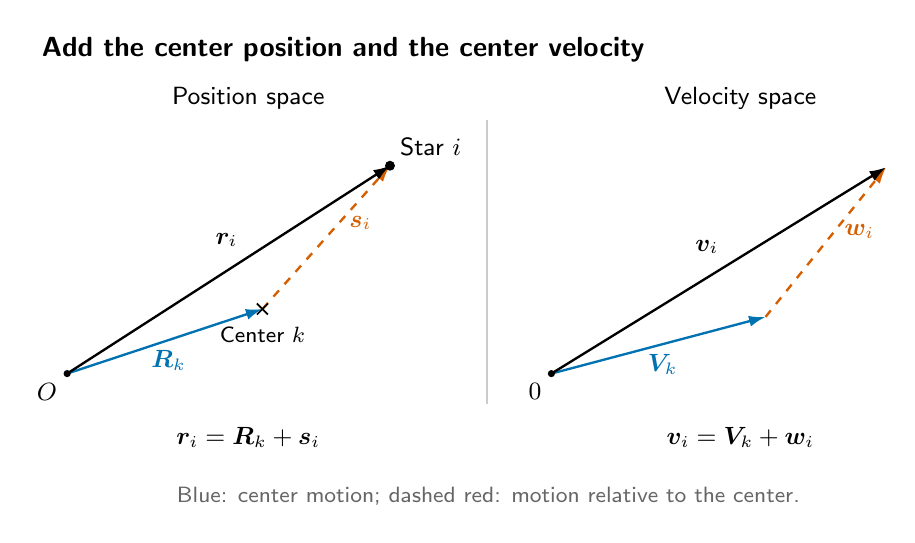
\begin{tikzpicture}[textbook diagram]
  \node[anchor=west,font=\sffamily\bfseries] at (0,4.80) {Add the center position and the center velocity};
  \node at (2.75,4.18) {Position space};
  \node at (9.00,4.18) {Velocity space};
  \coordinate (O) at (0.45,0.68); \coordinate (C) at (2.93,1.50); \coordinate (P) at (4.55,3.32);
  \coordinate (Z) at (6.60,0.68); \coordinate (V) at (9.32,1.40); \coordinate (W) at (10.85,3.30);
  \draw[vector,figblue] (O) -- node[below,pos=.52] {$\boldsymbol R_k$} (C);
  \draw[vector,figred,dashed] (C) -- node[right,pos=.60] {$\boldsymbol s_i$} (P);
  \draw[vector] (O) -- node[above left,pos=.56] {$\boldsymbol r_i$} (P);
  \draw[vector,figblue] (Z) -- node[below,pos=.52] {$\boldsymbol V_k$} (V);
  \draw[vector,figred,dashed] (V) -- node[right,pos=.57] {$\boldsymbol w_i$} (W);
  \draw[vector] (Z) -- node[above left,pos=.53] {$\boldsymbol v_i$} (W);
  \fill (O) circle(1.3pt);\node[below left] at (O) {$O$};
  \fill (Z) circle(1.3pt);\node[below left] at (Z) {$0$};
  \draw[black] ($(C)+(-.07,-.07)$) -- ($(C)+(.07,.07)$);\draw[black] ($(C)+(-.07,.07)$) -- ($(C)+(.07,-.07)$);
  \fill (P) circle(1.8pt);\node[above right] at (P) {Star $i$};
  \node[small label,below,yshift=-1.0mm] at (C) {Center $k$};
  \draw[black!20] (5.78,0.3) -- (5.78,3.9);
  \node at (2.75,-0.13) {$\boldsymbol r_i=\boldsymbol R_k+\boldsymbol s_i$};
  \node at (9.00,-0.13) {$\boldsymbol v_i=\boldsymbol V_k+\boldsymbol w_i$};
  \node[small label,text=figgray] at (5.80,-0.88) {Blue: center motion; dashed red: motion relative to the center.};
\end{tikzpicture}

\caption{局所円盤を慣性系へ移す二つのベクトル加算。位置には中心位置$\Rvec_k$、速度には中心速度$\Vvec_k$を加えます。朱色破線は中心に対する局所量です。左右は位置空間と速度空間の図なので、矢印の長さを相互に比較しません。}
\label{fig:concept-ch5-frame}
\end{figure}
\FloatBarrier
% END TikZ addition: ch05_frame_transform

\begin{failbox}{中心速度も足します}
位置にだけ$\Rvec_k$を足して、速度には$\Vvec_k$を足さないと、円盤が銀河中心と一緒に進みません。その後の崩れを潮汐相互作用の結果と判断してはいけません。初期値から$\rvec_i-\Rvec_k$と$\vvec_i-\Vvec_k$を計算し、局所円盤へ戻るか確認します。
\end{failbox}

\subsection{progradeの意味を定める}
第4章では円盤の向きを反時計回り・時計回りと呼びました。今回は二つの銀河の軌道があるので、円盤の角運動量と軌道の角運動量を比較できます。同じ向きの回転を\textbf{prograde}、逆向きを\textbf{retrograde}と呼びます。

標準軌道は$h>0$で反時計回りです。したがって、両円盤で\texttt{spin=+1}を選べばprograde--progradeの遭遇になります。$x$軸の右側・左側のどちらに銀河があるかではなく、\textbf{中心に対する局所的な回転の向き}で判断します。本章はまずこの一例を完成させ、向きを変える比較は章末の演習と第6章へ残します。


% BEGIN TikZ addition: ch05_spin_sense
図\ref{fig:concept-ch5-spin}は、軌道の向きを固定したまま円盤2の内部回転だけを変える比較です。中心の軌道方向を示す大きな矢印と、各円盤の回転を示す小さな矢印を区別してください。
\begin{figure}[!htbp]
\centering
% Sense-of-rotation sketch. The large curved arrows do NOT depict the center trajectories.
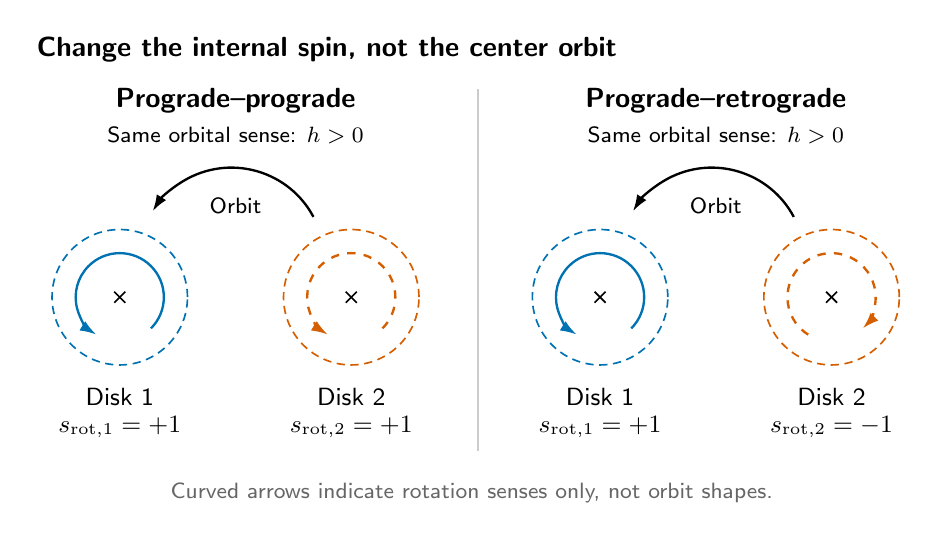
\begin{tikzpicture}[textbook diagram]
  \node[anchor=west,font=\sffamily\bfseries] at (0,4.70) {Change the internal spin, not the center orbit};
  \foreach \shift/\title/\mode in {0/Prograde--prograde/1,6.1/Prograde--retrograde/-1} {
    \begin{scope}[shift={(\shift,0)}]
      \node[font=\sffamily\bfseries] at (2.65,4.05) {\title};
      \node[small label] at (2.65,3.60) {Same orbital sense: $h>0$};
      \draw[vector,black] (3.64,2.57) arc[start angle=28,end angle=148,radius=1.18];
      \node[small label,fill=white,inner sep=1pt] at (2.65,2.71) {Orbit};
      \foreach \cx/\col/\id in {1.18/figblue/1,4.12/figred/2} {
        \draw[\col,densely dashed] (\cx,1.55) circle(.86);
        \draw[black] ({\cx-.07},1.48) -- ({\cx+.07},1.62);\draw[black] ({\cx-.07},1.62) -- ({\cx+.07},1.48);
        \node[below] at (\cx,.52) {Disk \id};
      }
      \draw[vector,figblue] (1.18,1.55) ++(-45:.56) arc[start angle=-45,end angle=238,radius=.56];
      \ifnum\mode=1
        \draw[vector,figred,dashed] (4.12,1.55) ++(-45:.56) arc[start angle=-45,end angle=238,radius=.56];
        \node at (4.12,-.10) {$s_{{\rm rot},2}=+1$};
      \else
        \draw[vector,figred,dashed] (4.12,1.55) ++(238:.56) arc[start angle=238,end angle=-45,radius=.56];
        \node at (4.12,-.10) {$s_{{\rm rot},2}=-1$};
      \fi
      \node at (1.18,-.10) {$s_{{\rm rot},1}=+1$};
    \end{scope}
  }
  \draw[black!20] (5.73,-.40) -- (5.73,4.2);
  \node[small label,text=figgray] at (5.65,-.93) {Curved arrows indicate rotation senses only, not orbit shapes.};
\end{tikzpicture}

\caption{軌道の向きを$h>0$に固定した回転方向の比較。左は両円盤がprograde、右は円盤2の内部回転だけがretrogradeです。大きな曲線矢印は軌道の回転の向きを示す記号で、中心軌道の形ではありません。回転は銀河中心に対する局所的な向きで判断します。}
\label{fig:concept-ch5-spin}
\end{figure}
\FloatBarrier
% END TikZ addition: ch05_spin_sense

\subsection{二銀河系の初期配置の近似を確認する}
局所の円運動速度は、出身銀河だけのPlummer場に対して決めています。有限の$D_0$から計算を始めるので、相手の銀河の重力は時刻0から加わります。したがって、これは孤立円盤二つを初期条件として配置したものであり、二銀河の合成場に対する厳密な平衡円盤ではありません。

初期距離を十分離して選ぶのは、この初期の摂動を抑えるためでもあります。ただし、相手の力を初めの数ステップだけ無視したり、説明なく徐々に強めたりはしません。式\eqref{eq:ch5-tracer-ode}の力を最初から一貫して使います。

\section{全体の配列を作り、同じ時刻へ進める}
\label{sec:ch5-integration}
\subsection{配列内の各行の役割を決める}
テスト粒子の合計を$N=N_1+N_2$とします。\texttt{state}は形$(2+N,4)$で、最初の2行を銀河中心、その後を円盤1と円盤2の星にします。
\begin{center}
\begin{tabular}{lll}
\toprule
Pythonの行 & 対象 & 列 \\
\midrule
\texttt{state[0]} & 銀河中心1 & \texttt{[x, y, vx, vy]} \\
\texttt{state[1]} & 銀河中心2 & 同上 \\
\texttt{state[2:2+N1]} & 円盤1のテスト粒子 & 同上 \\
\texttt{state[2+N1:]} & 円盤2のテスト粒子 & 同上 \\
\bottomrule
\end{tabular}
\end{center}

星にだけ対応する長さ$N$の整数配列\texttt{origin}も作ります。0が銀河1、1が銀河2の出身です。Pythonの番号は0から始まるので、本文の銀河番号より1小さい点に注意します。この出身番号は時間とともに変えません。他方の銀河の近くへ移った粒子も、同じ色と番号で追跡します。
\inputcode{chap05/assemble-state}

乱数生成器は一つだけ作り、円盤1、円盤2の順に使います。円盤ごとに同じseedへ戻して、全く同じ点配置を二つ作ることはしません。以後の時間刻み試験では、ここで得た初期配列を保存し、その同じ配列を使います。

\subsection{一度の呼び出しで全加速度を返す}
中心への加速度と星への加速度を、一つの関数へまとめます。ただし、その計算内容は分けたままです。
\inputcode{chap05/system-acceleration}

返り値は入力の\texttt{pos}と同じ形$(2+N,2)$です。先頭2行は式\eqref{eq:ch5-center-acceleration}、残りは式\eqref{eq:ch5-tracer-ode}です。後半の星の計算に\texttt{origin}は使いません。星の出身にかかわらず、二つの重力を足すためです。

中心同士の計算は1組だけです。星には二つの解析的な場を評価するだけなので、1回の全加速度計算は$O(N)$です。$N\times N$の距離表や、星の粒子対を走査する二重ループは作りません。

\subsection{KDKの更新式をそのまま使う}
第4章のKDKに、今作った加速度関数を渡します。
\inputcode{chap05/leapfrog-step}

最初の半kickで全行の速度を更新し、driftで全行の位置を更新します。その\texttt{pos\_new}には、星だけでなく\textbf{新しい銀河中心の位置}も入っています。そのため、次の加速度は新しい中心と新しい星の位置から計算されます。最後の半kickを終えると、全行の位置と速度が同じ整数時刻にそろいます。

\begin{failbox}{動く中心と星の時刻をずらさない}
中心だけを先に1ステップ進め、星には古い中心位置を使う処理では、ここで定めたKDKになりません。全行のdriftを終えてから、一つの位置配列を使って次の重力を求めます。描画用に間引いた中心の軌道を、時間積分の途中で代用することもしません。
\end{failbox}

力が位置から決まるので、この全行の更新を使えます。ただし、反作用を省いたテスト粒子を含む全配列を、通常の自己重力N体系と同一視しません。中心の二体系には保存量がありますが、星を加えた表示用のエネルギーの総和を、そのまま保存量にはできません。実際に確かめる量は\ref{sec:ch5-center-check}節と\ref{sec:ch5-energy}節で分けます。

\section{標準モデルを計算する}
\label{sec:ch5-standard}
\subsection{パラメータをそろえる}
本章の標準条件を表\ref{tab:ch5-standard}に示します。質量、Plummerスケール長、円盤分布は既存の標準モデルを引き継ぎます。二つの銀河を初期距離60 kpcから、目標近点8 kpcへ向かわせます。これらは教材用の値で、特定の観測銀河を再現するための調整ではありません。

\begin{table}[htbp]
\centering
\caption{第5章の標準モデル。長さの役割を区別します。全質量は$M_1+M_2=2\times10^{11}\Msun$で、テスト粒子に質量を加えません。}
\label{tab:ch5-standard}
\begin{tabular}{ll}
\toprule
量 & 設定 \\
\midrule
重力源 & $M_1=M_2=10^{11}\Msun$ \\
各Plummer場 & $a_1=a_2=3\unit{kpc}$ \\
中心間有効長さ & $b=3\unit{kpc}$ \\
円盤初期分布 & 両方$R_d=3\unit{kpc}$、$R_{\max}=15\unit{kpc}$ \\
粒子数・乱数 & $N_1=N_2=1000$、seed = 42 \\
CDF表 & 各円盤4096区間、4097分点 \\
中心軌道 & $D_0=60\unit{kpc}$、$D_p=8\unit{kpc}$、$\varepsilon=0$ \\
回転方向 & 軌道も両円盤も反時計回り \\
積分時間・時間刻み & $t_{\rm end}=0.60\unit{Gyr}$、$\Delta t=\chfivevalDt\unit{Myr}$ \\
ステップ数・保存 & \chfivevalNstep ステップ、星は\chfivevalSaveEvery ステップごと \\
\bottomrule
\end{tabular}
\end{table}

第4章の孤立円盤では$\Delta t=0.2\unit{Myr}$を使いました。本章では近接遭遇の後の粒子軌道も追うため、\textbf{時間刻みを$0.05\unit{Myr}$へ選び直します}。この選択は孤立円盤の誤差をそのまま流用したものではなく、\ref{sec:ch5-convergence}節の実際の刻み試験に基づきます。出力の間隔は2 Myrに保ちます。
\inputcode{chap05/parameters}

初期相対速度の成分は、式\eqref{eq:ch5-incoming-speed}から
\begin{equation}
U_r=\chfivevalVr\unit{km\,s^{-1}},\qquad U_t=\chfivevalVt\unit{km\,s^{-1}}
\label{eq:ch5-initial-values}
\end{equation}
となり、大きさは$\chfivevalSpeed\unit{km\,s^{-1}}$です。等質量なので各中心の初期位置は$(-30,0)$ kpcと$(30,0)$ kpcです。速度はそれぞれ相対速度の$-1/2$倍、$+1/2$倍になります。コード内部では速度をkpc/Gyrへ換算しています。

\subsection{中心と星で保存間隔を分ける}
近点時刻や保存量を調べるため、銀河中心の2行だけは毎ステップ保存します。星を含む全配列は40ステップごとに保存します。これは時間積分を分けるという意味ではありません。\textbf{計算は全行で同じ12000ステップ}を実行し、履歴へ書き込む頻度だけを分けます。
\inputcode{chap05/integrate-leapfrog}

\texttt{prepare\_history}は前章と同じ役割で、初期配列のコピー、保存ステップ番号、時間配列、保存領域を作ります。今回の初期配列は形$(2+N,4)$です。最後の時刻が保存間隔に一致しない場合も、必ず最終状態を保存します。補助的な入力確認のコードはNotebookに収録しています。

標準設定では、全履歴は$(301,2002,4)$、中心の履歴は$(12001,2,4)$です。\texttt{float64}の1要素を8 byteとして、配列だけの容量はそれぞれ\chfivevalHistoryMB\ MB、\chfivevalCenterMB\ MBです。MBは$10^6$ byteで数えています。一時配列、比較計算、図や動画の容量は別です。

全加速度関数の呼び出しは、初回1回と各ステップ1回で\textbf{\chfivevalForce 回}です。1回の呼び出しで、両中心と全テスト粒子の加速度を返します。粒子ごとの場の評価を数えた回数とは区別してください。実行時間はNotebookで測り、特定のノートPCでも同じ秒数になるとは仮定しません。

\section{まず銀河中心の軌道を確かめる}
\label{sec:ch5-center-check}
\subsection{中心二体系の保存量を求める}
テスト粒子からの反作用がないので、中心軌道は星の位置に依存しません。その二体系の全エネルギーは
\begin{equation}
E_{\rm c}=\frac12M_1V_1^2+\frac12M_2V_2^2-\frac{GM_1M_2}{\sqrt{D^2+b^2}}
\label{eq:ch5-center-energy}
\end{equation}
です。中心間のポテンシャルを1回だけ数えます。式\eqref{eq:ch5-pair-potential}で動かした中心に、点質量の$-GM_1M_2/D$を使ってエネルギーを診断しないようにします。

全運動量、原点の周りの全角運動量、重心位置は第2章と同じ
\begin{align}
\Pvec_{\rm c}&=M_1\Vvec_1+M_2\Vvec_2,\notag\\
L_{z,{\rm c}}&=M_1(\Rvec_1\times\Vvec_1)_z+M_2(\Rvec_2\times\Vvec_2)_z,\notag\\
\Rvec_{\rm cm}&=\frac{M_1\Rvec_1+M_2\Rvec_2}{\Mtot}
\label{eq:ch5-center-momentum}
\end{align}
です。$W_{\rm c}$は時間に陽には依存しない中心間のポテンシャルなので、$E_{\rm c}$は一定です。作用・反作用と中心力の関係から、$\Pvec_{\rm c}$と$L_{z,{\rm c}}$も保存され、重心は等速直線運動します。
\inputcode{chap05/center-diagnostics}

\subsection{初期値が0の量で割らない}
重心系の初期エネルギーは理論的には$E_{\rm c}(0)=0$、全運動量も0です。そこで、共通の正の規格化尺度を
\begin{align}
E_*&=\frac{GM_1M_2}{\sqrt{D_0^2+b^2}},&
V_*&=\sqrt{\frac{G\Mtot}{D_0}},\notag\\
P_*&=\Mtot V_*,&
L_*&=\mred D_0V_*,\qquad \mred=\frac{M_1M_2}{\Mtot}
\label{eq:ch5-error-scales}
\end{align}
とします。$V_*$は単位をそろえるための速度の尺度で、有効ポテンシャル中の円運動速度という意味ではありません。

各時刻での初期値からの差の最大値を、$E_*,L_*,P_*$でそれぞれ割り、$e_{E,{\rm c}},e_{L,{\rm c}},e_{P,{\rm c}}$とします。重心の誤差は
\begin{equation}
e_{\rm cm}=\max_n\frac{|\Rvec_{\rm cm}^n-[\Rvec_{\rm cm}(0)+t_n\Pvec_{\rm c}(0)/\Mtot]|}{D_0}
\label{eq:ch5-cm-error}
\end{equation}
です。最大値は、中心を保存した全ステップについて取ります。角運動量の誤差も今回は$L_*$で規格化するため、初期角運動量に対する相対誤差とは呼びません。

\begin{table}[htbp]
\centering
\caption{標準計算での銀河中心の保存量・重心のずれ。規格化は式\eqref{eq:ch5-error-scales}と式\eqref{eq:ch5-cm-error}です。丸め誤差に近い数値の末尾は環境により変わります。}
\label{tab:ch5-center-errors}
\begin{tabular}{lr}\toprule
指標 & 実測値 \\
\midrule
エネルギー $e_{E,{\rm c}}$ & $3.30\times 10^{-6}$ \\
角運動量 $e_{L,{\rm c}}$ & $5.19\times 10^{-15}$ \\
運動量 $e_{P,{\rm c}}$ & $0$ \\
重心位置 $e_{\rm cm}$ & $0$ \\
\bottomrule\end{tabular}

\end{table}

KDKのkickは一組の中心力から両方の速度を変えるため、全運動量と全角運動量を丸め誤差の範囲で保ちます。一方、エネルギーを厳密に保存する方法ではなく、$e_{E,{\rm c}}=\chfivevalEnergyError$のずれが残ります。表示される0は、この等質量・対称な初期条件と実装で得た結果であり、任意の条件でも厳密に0になるという意味ではありません。

\subsection{指定した近点への接近を確かめる}
図\ref{fig:ch5-separation}は銀河中心間距離の時間変化です。標準計算で保存された最小距離は$\chfivevalPeri\unit{kpc}$、その時刻は$\chfivevalTperi\unit{Gyr}$でした。目標の8 kpcへ近づいた後、両中心は離れていきます。
\begin{figure}[htbp]
\centering
\includegraphics[width=0.76\linewidth]{\figpath{ch05_separation}}
\caption{銀河中心間距離。破線は目標の近点8 kpc、四角は毎ステップの保存値の最小です。有限刻みの積分誤差と、真の近点時刻が保存時刻の間にある影響をともに含みます。}
\label{fig:ch5-separation}
\end{figure}

\begin{figure}[htbp]
\centering
\includegraphics[width=0.76\linewidth]{\figpath{ch05_center_energy}}
\caption{中心二体系の符号付きエネルギー差。近点付近で目立つ変化はKDKの有限刻みの効果です。動力学的摩擦を入れた軌道エネルギー損失ではありません。}
\label{fig:ch5-center-energy}
\end{figure}

中心の2行だけを取り出して、テスト粒子を全く置かずに再計算する試験も行います。今回の実装では中心の履歴は全要素で一致しました。星が多数あっても、中心へ反作用を返さないモデルになっていることを確認できます。

\FloatBarrier
\section{潮汐テイルとブリッジを見る}
本書の標準遭遇は、遠方の相手から弱い潮汐摂動を受ける場合ではなく、初期円盤の広がりが深く重なる強い近接遭遇です。目標近点距離$D_{\rm p}=8\unit{kpc}$は、各円盤の初期外縁$R_{\max}=15\unit{kpc}$より小さく、相手の中心が初期円盤の範囲内まで近づきます。この幾何学的な条件だけから、永久に失われる粒子割合は決まりません。以下では遠方展開ではなく、両Plummer場による運動を直接計算します。

\label{sec:ch5-tides}
\subsection{初期状態から近点通過後までを並べる}
図\ref{fig:ch5-snapshots}に四つの時刻を示します。青の丸は銀河1、朱色の三角は銀河2の出身粒子です。黒の$\times$と$+$がそれぞれのPlummer中心です。中心の印は重力場の位置を示すもので、Plummer場に追加した点質量ではありません。

\begin{figure}[htbp]
\centering
\includegraphics[width=0.49\linewidth]{\figpath{ch05_snapshot_000}}\hfill
\includegraphics[width=0.49\linewidth]{\figpath{ch05_snapshot_027}}\\[3mm]
\includegraphics[width=0.49\linewidth]{\figpath{ch05_snapshot_035}}\hfill
\includegraphics[width=0.49\linewidth]{\figpath{ch05_snapshot_050}}
\caption{標準のprograde--prograde遭遇。時刻は0、0.27、0.35、0.50 Gyrで、全図の軸範囲は$-90$から90 kpc、縦横比は1です。近点後には、初期の円盤から長く伸びる潮汐構造が見えます。色とマーカーは出身銀河に固定しています。Notebookには0.20、0.60 Gyrの図とアニメーションも保存しています。}
\label{fig:ch5-snapshots}
\end{figure}

初めはそれぞれの中心の周りに円盤があります。接近すると円盤が変形し、近点後には外側へ長く伸びる構造と、二つの中心の間をつなぐ構造が現れます。前者を\textbf{潮汐テイル}、後者を\textbf{潮汐ブリッジ}と呼びます。これらは本章の数値結果で粒子が集まって見える構造であり、ガスの衝撃波や新しく生まれた星を描いているのではありません。

\subsection{相手の重力と潮汐力を区別する}
銀河1の周りの星を考えます。相手の銀河2は、星だけでなく銀河1の中心も引きます。円盤の形を変えるのは、全体を同じように並進させる成分ではなく、\textbf{星と銀河中心が受ける加速度の差}です。ゼミで学んだ潮汐力の考え方に対応します。\cite{ryden2025}

本章の標準条件$a_1=a_2=b$では、銀河1の中心加速度は、銀河2のPlummer場を$\Rvec_1$で評価したものと一致します。$\boldsymbol s=\rvec_i-\Rvec_1$とすれば、中心に対する星の相対加速度は
\begin{equation}
\frac{d^2\boldsymbol s}{dt^2}
=\avec_1(\boldsymbol s)
+\underbrace{\left[\avec_2(\Rvec_1+\boldsymbol s)-\avec_2(\Rvec_1)\right]}_{\text{相手の銀河による加速度の差}}
\label{eq:ch5-tidal-difference}
\end{equation}
です。ここで$\avec_2$は銀河2の中心位置も含めて評価する場を表しています。$a_1,a_2,b$を独立に変更した場合には、中心への有効力と中心位置でのPlummer場が一致するとは限らないので、この差の書き方をそのまま流用しません。


% BEGIN TikZ addition: ch05_tidal_difference
図\ref{fig:concept-ch5-tide}では、相手からの加速度そのものと、中心の加速度を引いた差を分けています。遠い側の差が左向きでも、重力が斥力になったわけではありません。この差を、計算済みの両銀河の重力へもう一度足す必要もありません。
\begin{figure}[!htbp]
\centering
% Illustration along the line joining two well-separated galaxies.
% Only the companion's gravitational contribution is drawn.
% Arrow lengths use the point-mass far-field form. This is not the close-passage run.
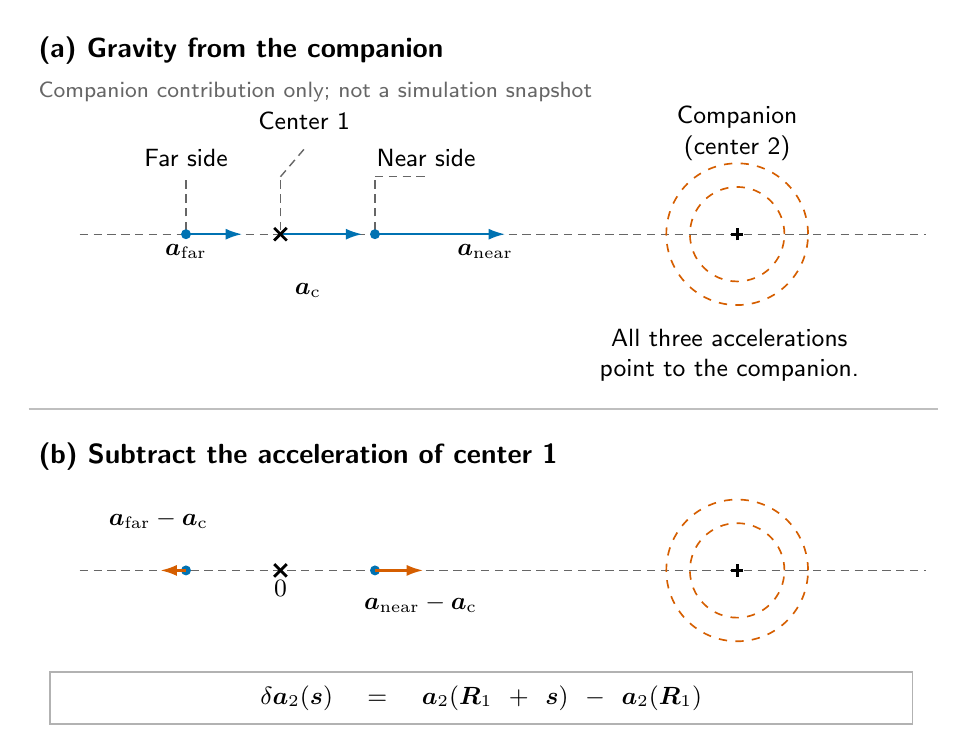
\begin{tikzpicture}[textbook diagram]
  \node[anchor=west,font=\sffamily\bfseries] at (0,4.05) {(a) Gravity from the companion};
  \node[small label,anchor=west,text=figgray] at (0,3.52) {Companion contribution only; not a simulation snapshot};
  \draw[guide] (0.65,1.72) -- (11.40,1.72);
  \foreach \x/\len/\lab in {2/0.71429/far,3.2/1.04043/c,4.4/1.65406/near} {
    \draw[vector,figblue] (\x,1.72) -- ++(\len,0);
    \draw[guide] (\x,1.77) -- (\x,2.45);
  }
  \fill[figblue] (2,1.72) circle (1.8pt);
  \fill[figblue] (4.4,1.72) circle (1.8pt);
  \draw[black,line width=1pt] (3.12,1.64) -- (3.28,1.80);
  \draw[black,line width=1pt] (3.12,1.80) -- (3.28,1.64);
  \node[above] at (2.0,2.45) {Far side};
  \node[above] at (3.5,2.92) {Center 1};
  \draw[guide] (3.2,2.45) -- (3.5,2.80);
  \node[above] at (5.05,2.45) {Near side};
  \draw[guide] (4.4,2.45) -- (5.05,2.45);
  \node[below] at (2.0,1.72) {$\boldsymbol a_{\rm far}$};
  \node[below,yshift=-5mm] at (3.55,1.72) {$\boldsymbol a_{\rm c}$};
  \node[below] at (5.80,1.72) {$\boldsymbol a_{\rm near}$};
  \draw[figred,dashed] (9.0,1.72) circle (0.60);
  \draw[figred,dashed] (9.0,1.72) circle (0.90);
  \draw[black,line width=1pt] (8.92,1.72) -- (9.08,1.72);
  \draw[black,line width=1pt] (9,1.64) -- (9,1.80);
  \node[align=center] at (9,3.0) {Companion\\(center 2)};
  \node[align=center] at (8.9,0.18) {All three accelerations\\point to the companion.};
  \draw[black!25] (0,-0.50) -- (11.55,-0.50);
  \node[anchor=west,font=\sffamily\bfseries] at (0,-1.10) {(b) Subtract the acceleration of center 1};
  \draw[guide] (0.65,-2.55) -- (11.40,-2.55);
  \fill[figblue] (2,-2.55) circle (1.8pt);
  \fill[figblue] (4.4,-2.55) circle (1.8pt);
  \draw[black,line width=1pt] (3.12,-2.63) -- (3.28,-2.47);
  \draw[black,line width=1pt] (3.12,-2.47) -- (3.28,-2.63);
  \draw[vector,figred] (2,-2.55) -- (1.67386,-2.55);
  \draw[vector,figred] (4.4,-2.55) -- (5.01363,-2.55);
  \node[above] at (1.65,-2.15) {$\boldsymbol a_{\rm far}-\boldsymbol a_{\rm c}$};
  \node[below] at (4.98,-2.73) {$\boldsymbol a_{\rm near}-\boldsymbol a_{\rm c}$};
  \node[below] at (3.2,-2.55) {$0$};
  \draw[figred,dashed] (9,-2.55) circle (0.60);
  \draw[figred,dashed] (9,-2.55) circle (0.90);
  \draw[black,line width=1pt] (8.92,-2.55) -- (9.08,-2.55);
  \draw[black,line width=1pt] (9,-2.63) -- (9,-2.47);
  \node[draw=black!30,fill=white,text width=106mm,align=center,inner sep=5pt] at (5.75,-4.17) {$\delta\boldsymbol a_2(\boldsymbol s)=\boldsymbol a_2(\boldsymbol R_1+\boldsymbol s)-\boldsymbol a_2(\boldsymbol R_1)$};
\end{tikzpicture}

\caption{相手銀河が十分遠い配置での説明図。上段は相手からの加速度、下段は銀河1の中心加速度を引いた差です。銀河1自身の重力は描いていません。$a_1=a_2=b$で中心加速度が対応する場合を考えています。近点8 kpcの標準計算のスナップショットではありません。}
\label{fig:concept-ch5-tide}
\end{figure}
\FloatBarrier
% END TikZ addition: ch05_tidal_difference

相手が十分遠く、$|\boldsymbol s|\ll D$かつ$D\gg a_2$なら、加速度の差の尺度は
\begin{equation}
|\delta\avec_2|\sim\frac{GM_2}{D^3}|\boldsymbol s|
\label{eq:ch5-tidal-scale}
\end{equation}
です。同じ相手までの距離でも、円盤の中心から離れた星ほど差を受けやすいことが分かります。また、円盤外側ほど出身銀河による束縛も弱くなります。ただし、式\eqref{eq:ch5-tidal-scale}だけでテイルの長さや向きが決まるわけではありません。遭遇中の星の回転と、時間に伴って変わる重力を積分した結果を見ます。

\begin{failbox}{潮汐力をもう一度足さない}
式\eqref{eq:ch5-tracer-ode}の二つの重力を使えば、星と中心が受ける重力の差はすでに含まれています。さらに「潮汐力」として別の加速度を足すと二重計算になります。また、本章の近点では円盤外縁15 kpcが中心間距離8 kpcより大きいため、円盤全体に$|\boldsymbol s|\ll D$の展開を使えません。実装は展開式ではなく、両Plummer場を直接評価します。
\end{failbox}

\subsection{出身粒子を拡大図で追跡する}
図\ref{fig:ch5-zoom}は同じ0.35 Gyrの結果を拡大したものです。円盤の内側だけを残して新たに計算したのではありません。中心の間にブリッジがあり、その外側へ曲がったテイルが伸びています。
\begin{figure}[htbp]
\centering
\includegraphics[width=0.76\linewidth]{\figpath{ch05_tidal_zoom}}
\caption{0.35 Gyrの拡大図。軸範囲は$\pm38$ kpcで、図\ref{fig:ch5-snapshots}とは異なります。矢印はブリッジとテイルの位置の例を示します。全体図と同じ粒子・同じ計算結果です。}
\label{fig:ch5-zoom}
\end{figure}

他方の銀河中心の近くに、異なる出身色の星が見えることもあります。しかし、近くへ来たことだけで、その銀河に永久に捕獲されたとは判断できません。ここではまず出身ラベルを保ったまま、どこへ移動したかを確認します。複雑な束縛判定やテイルの自動抽出は、本章には追加しません。

\FloatBarrier
\section{外へ移動した星を数える}
\label{sec:ch5-outer}
\subsection{何からの距離を測るかを決める}
図の見た目を補うため、出身銀河の中心から遠くへ移った粒子の割合を測ります。粒子$i$の出身銀河を$k(i)$と書くと、その距離は
\begin{equation}
s_i(t)=|\rvec_i(t)-\Rvec_{k(i)}(t)|
\label{eq:ch5-origin-radius}
\end{equation}
です。原点や、その時刻に最も近い銀河中心からの距離ではありません。

本章では閾値を$s_{\rm cut}=30\unit{kpc}=2R_{\max}$と定めます。各出身群$k$について
\begin{equation}
f_k(t)=\frac{1}{N_k}\sum_{i:\,k(i)=k}\boldsymbol{1}\left(s_i(t)>s_{\rm cut}\right)
\label{eq:ch5-outer-fraction}
\end{equation}
を計算します。$\boldsymbol{1}$は条件が真なら1、偽なら0です。初期配置の範囲は15 kpc以内なので、初期値では$f_1=f_2=0$です。
\inputcode{chap05/outer-fraction}

\texttt{history[:, origin, :2]}は、各テスト粒子の出身中心の位置を各時刻で取り出します。\texttt{history[:, 2:, :2]}と同じ$(N_{\rm save},N,2)$の形になるので、その差から距離を測れます。粒子を除去して分母を変える操作はしません。

\subsection{数値の意味と限界を確認する}
標準計算の0.60 Gyrでは、$f_1=\chfivevalOuterOne$、$f_2=\chfivevalOuterTwo$でした。1000粒子ずつの標本なので、各割合は0.001刻みです。二つは等質量・同じ分布モデルですが、有限の乱数標本が違うため、数値は完全には一致しません。
\begin{table}[htbp]
\centering
\caption{出身中心から30 kpcを越えた粒子の割合。これは位置による指標で、非束縛粒子や永久に剥ぎ取られた質量の割合ではありません。}
\label{tab:ch5-fractions}
\begin{tabular}{rrr}\toprule
$t\ [\mathrm{Gyr}]$ & $f_1$ & $f_2$ \\
\midrule
0.00 & 0.000 & 0.000 \\
0.20 & 0.000 & 0.000 \\
0.27 & 0.000 & 0.000 \\
0.35 & 0.023 & 0.017 \\
0.50 & 0.404 & 0.413 \\
0.60 & 0.425 & 0.432 \\
\bottomrule\end{tabular}

\end{table}
\begin{figure}[htbp]
\centering
\includegraphics[width=0.76\linewidth]{\figpath{ch05_outer_fraction}}
\caption{式\eqref{eq:ch5-outer-fraction}の時間変化。青実線と朱色破線が各出身群です。中心間距離が増えても、星の軌道はすぐに初期の円運動へ戻るわけではありません。}
\label{fig:ch5-fractions}
\end{figure}

この指標は\textbf{「外へ移動した割合」}です。出身銀河に束縛されたまま大きな軌道を回る粒子、後で戻る粒子、他の銀河の近くへ移った粒子も含み得ます。閾値30 kpcは本章で定めた測定条件であり、自然に一意に決まる潮汐半径ではありません。「剥ぎ取りが起こり得る様子」を見ることと、永久に失われた質量を定量的に予測することを区別します。

\FloatBarrier
\section{星のエネルギーが変化する理由を考える}
\label{sec:ch5-energy}
第4章では固定した一つのPlummer場を使ったため、各星の比エネルギーが保存されました。今回は両中心が動きます。慣性系での比エネルギーを
\begin{equation}
\varepsilon_i(t)=\frac12|\vvec_i(t)|^2+\Phi_1(\rvec_i,t)+\Phi_2(\rvec_i,t)
\label{eq:ch5-tracer-energy}
\end{equation}
と定義しても、一般には一定ではありません。

運動方程式を使って時間微分すると、$\vvec_i\cdot\avec_i$と$\vvec_i\cdot\nabla\Phi$が打ち消し合い、
\begin{equation}
\frac{d\varepsilon_i}{dt}=\frac{\partial\Phi}{\partial t}
=\sum_{k=1}^2\Vvec_k\cdot\avec_{k,i}
\label{eq:ch5-energy-rate}
\end{equation}
が残ります。最後の等号は、$\Phi_k$が$\rvec_i-\Rvec_k(t)$の関数で、$M_k,a_k$は一定であることから得られます。これは本章のモデルの式を微分した関係です。\textbf{動力学的摩擦を入れなくても、動く重力場は星のエネルギーを変えます。}
\inputcode{chap05/tracer-energy}

図\ref{fig:ch5-tracer-energy}では、銀河1の出身粒子のうち、初期半径が$3R_d=9$ kpcに最も近い1粒子を選びました。その初期半径は$\chfivevalWatchRadius\unit{kpc}$です。これは個別の軌道の例で、星全体の平均値ではありません。
\begin{figure}[htbp]
\centering
\includegraphics[width=0.76\linewidth]{\figpath{ch05_tracer_energy}}
\caption{選んだ1粒子の比エネルギー変化。規格化は$GM_1/a_1$です。図\ref{fig:ch5-center-energy}の「中心の保存量の誤差」と違い、こちらの変化には時間依存する場の物理的な効果が含まれます。}
\label{fig:ch5-tracer-energy}
\end{figure}

星へのトルクも一般には0ではないので、慣性系の原点の周りの各星の角運動量も保存しません。また、星から中心へ反作用を返していないため、星の表示上の重みにエネルギーを掛け、その和を$E_{\rm c}$へ足して「全系の保存量」とすることはできません。今回の確認では、\textbf{中心の二体系の保存量}と、\textbf{星の位置の時間刻み依存性}を分けます。

\section{相互作用計算の時間刻みを確認する}
\label{sec:ch5-convergence}
\subsection{初期粒子も評価時刻も固定する}
二銀河が動く間の星には、第4章の孤立円盤の円軌道の解析位置は使えません。その位置からずれた量には、意図した相互作用の効果が入るためです。ここでは第3章の非円軌道と同じく、\textbf{同じモデルの、異なる刻みの数値解どうし}を比較します。

初期配列、終時刻0.60 Gyr、評価する151個の時刻を固定します。ステップ数だけを3000、6000、12000、24000とし、刻みは0.20、0.10、0.05、0.025 Myrです。比較時刻を4 Myrごとにそろえるため、各計算で\texttt{save\_every = n\_steps // 150}とします。この保存設定は、標準図の301時刻とは別の検証用設定です。

\begin{table}[htbp]
\centering
\caption{刻みごとの中心軌道と0.60 Gyrの外側粒子割合。$D_{\min}$と$e_{E,{\rm c}}$は中心の全ステップから求めています。$f_1,f_2$の閾値は30 kpcです。}
\label{tab:ch5-resolution}
\small\begin{tabular}{rrrrrr}\toprule
$N_{\rm step}$ & $\Delta t\ [\mathrm{Myr}]$ & $D_{\min}\ [\mathrm{kpc}]$ & $e_{E,{\rm c}}$ & $f_1$ & $f_2$ \\
\midrule
3000 & 0.200 & 8.000109881 & $5.28\times 10^{-5}$ & 0.425 & 0.432 \\
6000 & 0.100 & 8.000014569 & $1.32\times 10^{-5}$ & 0.425 & 0.432 \\
12000 & 0.050 & 8.000004531 & $3.30\times 10^{-6}$ & 0.425 & 0.432 \\
24000 & 0.025 & 8.000001962 & $8.26\times 10^{-7}$ & 0.425 & 0.432 \\
\bottomrule\end{tabular}

\end{table}

中心の最小距離は8 kpcへ近づき、エネルギー誤差も刻みを細かくするにつれて減ります。一方、この表では外側粒子の割合が全行で同じ値でした。しかし、その一致だけで各星の位置まで正確だとは判断できません。割合は粒子が閾値のどちら側にいるかだけを数え、個々の位置の違いを捨てる量だからです。

\subsection{隣接する刻みの位置の差を測る}
粗い刻みを$\Delta t$、細かい刻みを$\Delta t/2$と書きます。評価する各時刻$t_j$で位置の差を取り、中心と星について
\begin{align}
\delta_{\rm c}(\Delta t)&=\max_{j,k}\frac{|\Rvec_{k,\Delta t}(t_j)-\Rvec_{k,\Delta t/2}(t_j)|}{D_0},\notag\\
\delta_{\rm t}(\Delta t)&=\max_{j,i}\frac{|\rvec_{i,\Delta t}(t_j)-\rvec_{i,\Delta t/2}(t_j)|}{R_d}
\label{eq:ch5-self-difference}
\end{align}
を求めます。これは真の解との誤差ではなく、二つの数値解の差です。同じ時刻・同じ粒子番号で比較します。粒子を位置順に並べ替えてから対応させることはしません。

少数の軌道に大きな差が集中する場合を見分けるため、星については二乗平均平方根の差も求めます。
\begin{equation}
\delta_{\rm rms}(\Delta t)=\frac{1}{R_d}
\sqrt{\frac{1}{N_{\rm eval}N}\sum_{j,i}|\rvec_{i,\Delta t}(t_j)-\rvec_{i,\Delta t/2}(t_j)|^2}.
\label{eq:ch5-rms-difference}
\end{equation}
$N_{\rm eval}=151$、$N=2000$です。最大値と平均的な大きさの両方を残し、一方だけで精度を説明しないようにします。
\inputcode{chap05/time-convergence}

\begin{table}[htbp]
\centering
\caption{151個の共通時刻での位置の自己収束。左の2列はステップ数です。前行との比は$\delta_{\rm t}$から求めています。$\delta_{\rm rms}$は星・評価時刻の両方にわたる二乗平均平方根です。}
\label{tab:ch5-self-convergence}
\small\begin{tabular}{rrrrrr}\toprule
粗い計算 & 細かい計算 & $\delta_{\rm c}$ & $\delta_{\rm t}$ & $\delta_{\rm rms}$ & 前行との比 \\
\midrule
3000 & 6000 & $3.90\times 10^{-6}$ & $2.51\times 10^{-1}$ & $2.68\times 10^{-3}$ & --- \\
6000 & 12000 & $9.75\times 10^{-7}$ & $6.41\times 10^{-2}$ & $6.71\times 10^{-4}$ & 3.92252 \\
12000 & 24000 & $2.44\times 10^{-7}$ & $1.61\times 10^{-2}$ & $1.68\times 10^{-4}$ & 3.97963 \\
\bottomrule\end{tabular}

\end{table}

最も細かい比較では、最大差$\delta_{\rm t}=\chfivevalLastDifference$、二乗平均平方根は$\delta_{\rm rms}=\chfivevalLastRMS$でした。$R_d=3$ kpcなので、最大の位置差はおよそ$\chfivevalLastDifferenceKpc$ kpcです。二つの値の違いは、一部の粒子が全体の平均より刻みに敏感であることを示します。

\begin{figure}[htbp]
\centering
\includegraphics[width=0.76\linewidth]{\figpath{ch05_convergence}}
\caption{隣接する刻みの星の位置の差。青丸が最大値、朱色四角が二乗平均平方根です。灰色破線は最も細かい比較の最大値を通る傾き2の参照線で、実測点への当てはめではありません。}
\label{fig:ch5-convergence}
\end{figure}

解の主な誤差が$C(\Delta t)^2$で表せる範囲なら、隣接する解の差は$(3/4)C(\Delta t)^2$です。その差どうしの比は約4になります。表\ref{tab:ch5-self-convergence}の細かい側では比が\chfivevalLastRatio となり、4へ近づいています。標準の0.05 Myrは、この比較で潮汐形態と外側割合を調べるための基準とします。すべての粒子の真の軌道誤差が一定値以下だと保証する設定ではありません。より長い計算、より小さい近点、別の密度集中度へ変更したら、刻みも再確認します。

\subsection{一致する数値の意味を確かめる}
自己収束だけでは、加速度の式そのものが正しいことを証明できません。中心間力の作用・反作用、星への重力の和、中心軌道だけの独立計算、単独Plummer場中の円盤の検証を組み合わせます。これらの独立な確認コードも配布物に含めています。

全中心・全星に同じ初期位置$(5,-3)$ kpcと速度$(30,-20)$ km/sを加える試験も行います。相対位置は変わらないので、同じ相対運動になるはずです。今回の出身中心に対する粒子位置の差は、$R_d$で規格化した最大値で$\chfivevalBoostDiff$でした。標準の刻みを変えた差より十分小さくなっています。ただし、軌道が摂動に敏感な場合には丸めの違いも時間とともに増え得るので、任意の計算で同じ数値になるとは考えません。

\FloatBarrier
\section{このモデルで分かることと限界を整理する}
\label{sec:ch5-limits}
本章の計算から、二つの銀河が接近すると、星の軌道が変わり、円盤からテイルやブリッジが生じる様子を確認できました。新しい星を生成したわけではなく、初めからあった星を別の位置へ運んだ結果です。また、星のエネルギーが変化しても、中心の二体系の軌道エネルギーは保存されるモデルだと確認しました。

中心が再び離れていくことは計算の失敗ではありません。$\varepsilon=0$の中心軌道に摩擦や星からの反作用がないので、近接通過後に自動的に合体へ切り替わる仕組みはありません。ポテンシャルの形も質量も固定なので、潮汐変形を受けて銀河の重力場自体が変わる過程、質量損失に伴う中心軌道の変化、合体残骸が落ち着く過程は扱っていません。

また、円盤と遭遇軌道は同じ平面に置いています。円盤の傾斜角、厚み、鉛直方向の運動は扱いません。したがって、後のprograde--retrogradeの比較は共面配置で内部回転の向きだけを変える実験です。任意の傾斜を持つ銀河遭遇の形態まで、この二つの向きだけで分類することはできません。

次の第6章では、完成したコードを用い、近点距離、質量比、円盤の回転方向を一つずつ変えます。さらに発展では、衛星銀河の中心へChandrasekhar動力学的摩擦を加え、軌道減衰を調べます。その速度依存力にはRK4を使います。摩擦を質量ゼロの星一つずつへ掛けるわけではありません。ここまでの重力だけの計算を基準として、何を追加したかを明確にします。

\section{本章のまとめ}
本章では、2中心と多数のテスト粒子を一つの配列へまとめました。中心同士は共通の有効対ポテンシャルで動かし、星には二つの移動するPlummer場を足しました。中心間の有効力と、広がった密度分布間の厳密な相互力は区別しました。

初期軌道は、採用したポテンシャルの比エネルギーと比角運動量から求めました。各円盤は第4章の方法で作り、位置と速度の両方に中心の運動を加えました。KDKでは全中心・全粒子をそろえて更新し、新しい中心位置を使って星の加速度を求め直しました。

結果には潮汐テイルとブリッジが現れました。これらを重力の差による軌道の変化として読み、出身中心から遠くへ移動した星の割合も測りました。ただし、その割合を非束縛率や質量損失率とは呼びません。中心の保存量、星の位置の自己収束、異なる座標系での比較を使い、図の見た目だけで検証を終えないことを確認しました。

\chapterexercises
\paragraph{演習5.1　確認：どの重力を計算するか}
中心1、中心2、銀河1出身の星、銀河2出身の星の加速度をそれぞれ書いてください。$M_1\ne M_2$、$a_1\ne a_2$の場合でも、共通の$b$を使った中心間力が作用・反作用を満たすことを示してください。\texttt{origin}を星の重力源の選別に使ってはいけない理由も述べてください。

\paragraph{演習5.2　確認：有効軌道の初期条件}
表\ref{tab:ch5-standard}の値から、$h,U_t,U_r$を求め、$\varepsilon(0)=0$を確認してください。同じ$h$で$D=D_p$としたとき、動径速度が0になることも確かめてください。$b\to0$の極限で、第2章の放物線の式へ戻ることを示してください。

\paragraph{演習5.3　確認：円盤の並進}
\texttt{place\_disk}の出力から中心位置と中心速度を引き、元の局所円盤へ戻ることを確認してください。中心速度を足し忘れた場合、各粒子の中心に対する速度にどの項が加わるでしょうか。その崩れを、正しい潮汐テイルの再現と判断できるでしょうか。

\paragraph{演習5.4　応用：時間刻みと誤差指標}
同じ初期配列で表\ref{tab:ch5-resolution}と表\ref{tab:ch5-self-convergence}を再計算してください。外側割合が同じ値でも最大位置差が0ではない理由を説明してください。自己収束の差を真の軌道誤差と区別し、標準設定を変更した場合に再確認すべきものを挙げてください。

\paragraph{演習5.5　応用：保存間隔だけを変える}
標準の時間刻みを固定します。\texttt{save\_every}を1、40、200として比べてください。全粒子の最終状態、毎ステップの中心履歴、全履歴の容量はどう変わりますか。出力の細かさと時間積分の精度を区別してください。メモリが少ない場合は、粒子数を減らしてから三つの保存設定を比較して構いません。

\paragraph{演習5.6　応用：系全体を等速で動かす}
すべての中心と星に、同じ初期位置$(5,-3)$ kpcと速度$(30,-20)$ km/sを加えてください。出身中心からの相対位置と中心間距離を、もとの計算と比べてください。慣性系での各星のエネルギーの数値まで、もとの計算と一致する必要があるでしょうか。

\paragraph{演習5.7　発展：片方の円盤を逆回転にする}
標準の初期位置と中心の初期速度を保ち、銀河2出身の星の\textbf{中心に対する速度だけ}を反転してください。0.60 Gyrの粒子分布と$f_1,f_2$を比べてください。星の速度全体へ単に$-1$を掛けた場合とは何が違いますか。中心軌道と銀河1出身の星の軌道が変わらないことも確認してください。この比較を、自己重力銀河全体の逆回転合体の定量的予測とみなしてよいでしょうか。

\newcommand{\chsixvalBaseOne}{0.390}
\newcommand{\chsixvalBaseTwo}{0.401}
\newcommand{\chsixvalRetroTwo}{0.055}
\newcommand{\chsixvalSpinDifference}{0.346}
\newcommand{\chsixvalBaseTime}{0.470}
\newcommand{\chsixvalBaseTau}{0.200100}
\newcommand{\chsixvalQsmallTime}{0.363900}
\newcommand{\chsixvalFinalPPTwo}{0.432}
\newcommand{\chsixvalFinalPRTwo}{0.065}
\newcommand{\chsixvalPeriSeries}{0.352,0.401,0.299}
\newcommand{\chsixvalMassSeriesOne}{0.390,0.225,0.000}
\newcommand{\chsixvalMassSeriesTwo}{0.401,0.544,0.427}
\newcommand{\chsixvalSmallTauFixed}{0.106100}
\newcommand{\chsixvalEpochDifferenceMyr}{94}
\newcommand{\chsixvalThresholdDifferences}{0.355,0.346,0.276}
\newcommand{\chsixvalSeedDifferences}{0.346,0.349,0.361}
\newcommand{\chsixvalPfiveMax}{1.25\times 10^{-2}}
\newcommand{\chsixvalPfiveRms}{2.07\times 10^{-4}}
\newcommand{\chsixvalSoftFive}{0.631}
\newcommand{\chsixvalSoftRatios}{0.631,0.821,0.913}

\chapter{銀河相互作用を調べる}
\label{chap:experiments}
第5章では、二つの移動するPlummerポテンシャルとテスト粒子円盤を組み合わせ、銀河相互作用を計算しました。本章では、完成したコードを数値実験の道具として使います。円盤の回転方向、近点距離、質量比を別々に変え、何が変わり、何が変わらないかを調べます。新しい重力積分器を作るのではなく、前章のKDK leapfrogを再利用します。

\begin{goalbox}[この章で学ぶこと]
\begin{itemize}
\item 変更するパラメータ、固定する条件、測定する量を、計算前に決められます。
\item 同じ初期標本を使い、prograde・retrograde、近点距離、質量比の比較ができます。
\item 近点からの経過時間をそろえ、粒子割合と形態の違いを説明できます。
\item 時間刻み、乱数標本、測定条件への依存を、物理モデルの変更と区別できます。
\end{itemize}
\end{goalbox}

\section{計算を数値実験として組み立てる}
\label{sec:ch6-design}
\subsection{まず問いを一つ決める}
「銀河を接近させると何かが起きる」という確認から、もう一歩進みます。例えば、「円盤2の回転を逆向きにすると、出身中心から遠くへ移る星の割合は変わるでしょうか」という問いを立てます。この問いに答えるには、回転以外の条件をそろえる必要があります。

同時に、何をもって違いを判断するかも決めます。本章では、同じ範囲で描いた粒子分布と、第5章の外側粒子割合を使います。図を見てから都合のよい時刻や閾値だけを選ぶのではなく、標準の測定条件を先に定めます。別の条件でも確認するときには、それを追加の試験として区別します。

\subsection{一つの変更が初期値に及ぼす影響を確認する}
独立に指定するパラメータを一つ変えても、すべての配列要素が一つだけ変わるわけではありません。近点距離を変えれば、それを実現する初期接線速度と動径速度も変わります。銀河の質量を変えれば、中心軌道だけでなく、その銀河の円運動速度も変わります。

ここでいう「一つずつ変える」は、こうした連動を止めることではありません。変更する入力と、モデルの式から計算し直す値を区別することです。表\ref{tab:ch6-design}に、本章で行う三つの系列を示します。
\begin{table}[htbp]\centering\small
\caption{基本編の比較系列。すべて第5章と同じ重力モデルを使います。質量比系列では全質量を固定しません。}\label{tab:ch6-design}
\begin{tabularx}{\linewidth}{lXX}\toprule
系列 & 直接変更するもの & 連動して作り直すもの \\\midrule
回転方向 & 円盤2の内部回転 $s_{{\rm rot},2}=+1,-1$ & 円盤2の中心に対する速度 \\
近点距離 & $D_{\rm p}=5,8,12\unit{kpc}$ & 中心の初期相対速度 \\
質量比 & $M_1$を固定した $q=M_2/M_1$ & 中心の初期位置・速度、円盤2の円運動速度 \\\bottomrule
\end{tabularx}
\end{table}

\begin{failbox}{名前だけを変えても、軌道は変わりません}
計算済みの初期状態を保ったまま、変数\texttt{d\_peri}だけを書き換えても、実際の近点距離は変わりません。近点距離は積分器へ毎ステップ与える命令ではなく、初期速度を決めるための入力です。質量を変更した場合も、必要な初期値を同じモデルから作り直します。
\end{failbox}

\section{第5章の基準と測定方法を引き継ぐ}
\label{sec:ch6-baseline}
\subsection{基準モデルを再現する}
基準モデルは、$M_1=M_2=10^{11}\Msun$、$a_1=a_2=b=3\unit{kpc}$、各円盤$N_k=1000$粒子、$R_{\rm d}=3\unit{kpc}$、$R_{\max}=15\unit{kpc}$です。中心間の初期距離は$60\unit{kpc}$、目標近点距離は$8\unit{kpc}$で、両円盤をprogradeとします。円盤生成には前章と同じseed、乱数の呼び出し順序、CDF表を使います。

内部単位はkpc、Gyr、$\Msun$です。時間積分は$0.60\unit{Gyr}$まで、刻みは$0.05\unit{Myr}$です。全粒子は2 Myrごと、中心は毎ステップ保存します。KDKの新しい加速度評価は、1計算につき$12000+1=12001$回です。各ステップで全中心・全粒子を同じ時刻へ進めます。
\inputcode{chap06/base-config}

\texttt{dict}は、パラメータを名前と値の組でまとめるPythonの辞書です。質量の配列は\texttt{base\_config}からキー\texttt{"masses"}を指定して取り出します。新しいクラスは作りません。比較用の辞書は\texttt{dict(...)}で作り、変更しない配列はそのまま参照します。本章の関数は入力配列を上書きしないため、この使い方ができます。

コードは第5章の関数定義をNotebook内にも収録しています。別の章のNotebookを先に実行する必要はありません。一方、本文では円盤のCDF、Plummer加速度、KDKの導出を繰り返しません。式と実装の確認には前章までを参照します。（第\ref{chap:interaction}章参照）

\subsection{出身中心から外へ移った割合を使う}
粒子$i$の出身銀河を$k(i)$とし、出身中心からの距離を
\begin{equation}
 s_i(t)=|\rvec_i(t)-\Rvec_{k(i)}(t)|
 \label{eq:ch6-origin-radius}
\end{equation}
とします。初期に付けた出身番号は、他方の中心へ近づいても変更しません。閾値を$s_{\rm cut}=30\unit{kpc}$とし、各出身群について
\begin{equation}
 f_k(t)=\frac{1}{N_k}\sum_{i:k(i)=k}\mathbf{1}\bigl(s_i(t)>s_{\rm cut}\bigr)
 \label{eq:ch6-fraction}
\end{equation}
を測ります。$\mathbf{1}$は条件が真なら1、偽なら0です。前章の\texttt{origin\_radii}と\texttt{outer\_fractions}を、そのまま使います。

この量は位置だけで定義した割合です。非束縛率、永久に剥ぎ取られた割合、質量損失率とは呼びません。$N_k$は重力源の質量を分割した数でもありません。例えば質量比1:10でも各円盤1000粒子を置き、両出身群を同じ標本数で表示できます。

\subsection{近点からの経過時間をそろえる}
近点距離や全質量を変えると、近点通過の時刻も変わります。同じ$t=0.40\unit{Gyr}$の図でも、一方は接近直後、他方はまだ接近中かもしれません。そこで、本章の主な比較には
\begin{equation}
 \tau=t-t_{\rm p}
 \label{eq:ch6-aligned-time}
\end{equation}
を使います。$t_{\rm p}$は、毎ステップ保存した中心間距離の最小値に対応する時刻です。連続時間の厳密な近点時刻ではありません。

比較表では$\tau=0.20\unit{Gyr}$を目標にします。星の履歴は2 Myrごとなので、目標に最も近い保存時刻を使い、実際の$t$と$\tau$も記録します。保存間隔が一定なら、この選択による目標時刻との差は1 Myr以下です。この上限は、中心の近点時刻自体の数値誤差を含む上限ではありません。
\inputcode{chap06/aligned-index}

\texttt{np.argmin}が返すのは配列内の最小値の場所です。距離の最小が計算の端にある場合や、比較したい時刻が保存範囲を外れる場合には、そのまま比較を続けず停止します。別のモデルで$\tau=0.20\unit{Gyr}$まで到達していなければ、計算時間を延ばすか、全系列の比較時刻を変更します。


% BEGIN TikZ addition: ch06_time_alignment
図\ref{fig:concept-ch6-time}で、二つの実験の近点時刻をそろえる操作を確認してください。目標の$\tau$と実際に使った保存時刻は区別し、両者を記録します。
\begin{figure}[!htbp]
\centering
% Schematic timing only. The benchmark's pericenter is measured from sampled center positions.
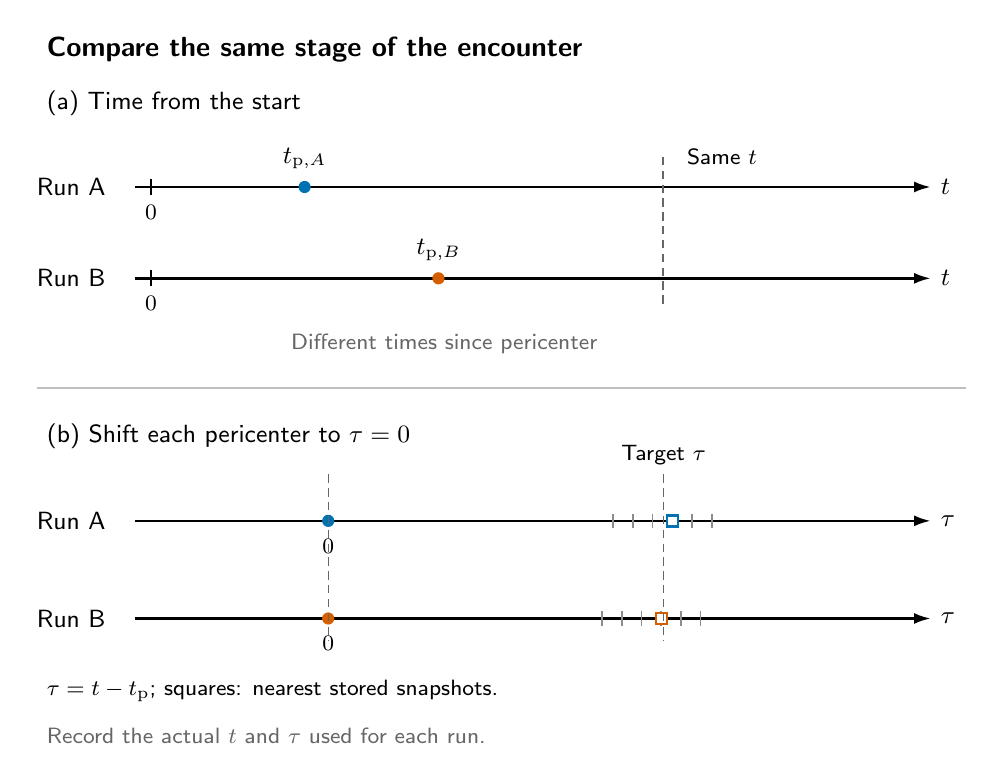
\begin{tikzpicture}[textbook diagram]
  \node[anchor=west,font=\sffamily\bfseries] at (0,4.73) {Compare the same stage of the encounter};
  \node[anchor=west] at (0,4.04) {(a) Time from the start};
  \foreach \y/\tag/\p/\col in {2.98/A/3.4/figblue,1.82/B/5.1/figred} {
    \node[anchor=east] at (1.0,\y) {Run \tag};
    \draw[vector] (1.25,\y) -- (11.35,\y) node[right] {$t$};
    \draw (1.45,{\y-.10}) -- (1.45,{\y+.10});\node[below,small label] at (1.45,{\y-.10}) {$0$};
    \fill[\col] (\p,\y) circle (2.2pt);
    \node[above] at (\p,{\y+.10}) {$t_{{\rm p},\tag}$};
  }
  \draw[guide] (7.95,1.5) -- (7.95,3.43);
  \node[small label,anchor=west] at (8.13,3.36) {Same $t$};
  \node[small label,text=figgray,anchor=west] at (3.10,.99) {Different times since pericenter};
  \draw[black!25] (0,.43) -- (11.80,.43);
  \node[anchor=west] at (0,-.18) {(b) Shift each pericenter to $\tau=0$};
  \foreach \y/\tag/\col/\sel in {-1.26/A/figblue/8.07,-2.50/B/figred/7.93} {
    \node[anchor=east] at (1.0,\y) {Run \tag};
    \draw[vector] (1.25,\y) -- (11.35,\y) node[right] {$\tau$};
    \fill[\col] (3.7,\y) circle (2.2pt);
    \node[below,small label] at (3.7,{\y-.10}) {$0$};
    \foreach \delta in {-.75,-.50,-.25,0,.25,.50} {\draw[black!45] ({\sel+\delta},{\y-.09}) -- ({\sel+\delta},{\y+.09});}
    \draw[\col,fill=white,line width=.9pt] ({\sel-.07},{\y-.07}) rectangle ({\sel+.07},{\y+.07});
  }
  \draw[guide] (3.7,-.67) -- (3.7,-2.78);
  \draw[guide] (7.96,-.67) -- (7.96,-2.78);
  \node[small label,above] at (7.96,-.68) {Target $\tau$};
  \node[small label,anchor=west] at (0,-3.42) {$\tau=t-t_{\rm p}$; squares: nearest stored snapshots.};
  \node[small label,text=figgray,anchor=west] at (0,-3.99) {Record the actual $t$ and $\tau$ used for each run.};
\end{tikzpicture}

\caption{開始からの時刻$t$と、近点からの経過時間$\tau=t-t_{\rm p}$の違い。下段では各近点を$\tau=0$へそろえています。小目盛りは保存時刻、四角は目標に最も近い保存時刻です。配置と目盛りは説明用で、実測の時間間隔を表していません。}
\label{fig:concept-ch6-time}
\end{figure}
\FloatBarrier
% END TikZ addition: ch06_time_alignment

\subsection{一回の実験を短い関数にまとめる}
初期値、KDK、診断という既習の順序を関数へまとめます。返す辞書には、設定と結果を一緒に入れます。比較後に、どの曲線がどの条件だったか分からなくなることを避けられます。
\inputcode{chap06/run-case}

\texttt{make\_initial\_state(**config)}は、辞書内の名前付きパラメータを関数へ渡す記法です。\texttt{*args}は、ここでは質量、Plummerスケール、有効長さの三つを順に渡します。どちらも新しい数値計算法ではなく、引数の整理です。関数が返す位置や速度を、後から「保存則に合うように」修正する操作は行いません。

\section{円盤の回転方向を変える}
\label{sec:ch6-spin}
\subsection{銀河中心の運動を固定する}
回転方向の定義は図\ref{fig:concept-ch5-spin}を参照してください。ここでも変えるのは円盤2の内部回転だけです。

基準のprograde--progradeをPP、円盤2だけをretrogradeにしたものをPRと呼びます。軌道の比角運動量は正で、反時計回りです。円盤2の回転を変えるときには、局所的な内部速度だけを反転します。
\begin{equation}
 \vvec_i'=\Vvec_2-(\vvec_i-\Vvec_2)=2\Vvec_2-\vvec_i
 \quad\bigl(k(i)=2\bigr).
 \label{eq:ch6-reverse-spin}
\end{equation}
中心の速度$\Vvec_2$は変えません。全速度に単に$-1$を掛けると、銀河全体の並進運動まで反転してしまいます。
\inputcode{chap06/reverse-spin}

同じseed・粒子数から円盤を生成すると、PPとPRの初期位置は同じで、円盤2の内部速度だけが反転します。配列から式\eqref{eq:ch6-reverse-spin}を直接計算した結果とも照合します。

本モデルでは、円盤粒子から中心への反作用がありません。また、円盤2の星から円盤1の星への力もありません。このため、PPとPRで中心軌道と円盤1の全粒子軌道は同じになります。配布コードでも配列の一致を確認します。これは一般の自己重力銀河でも成り立つ性質ではなく、本書の近似に由来します。（第\ref{chap:interaction}章参照）

\subsection{形と割合を合わせて読む}
図\ref{fig:ch6-pp}と図\ref{fig:ch6-pr}は、$\tau\simeq0.20\unit{Gyr}$での比較です。位置の表示範囲、出身色、マーカー、粒子数をそろえています。PRの円盤2では、PPと比べて遠方まで伸びた粒子の数が少なく見えます。
\begin{figure}[htbp]\centering
\includegraphics[width=0.63\linewidth]{\figpath{ch06_pp}}
\caption{PPの粒子分布。青丸と朱色三角はそれぞれ銀河1・2の出身粒子です。黒い$\times,+$はPlummer中心です。実際の比較時刻は$t=\chsixvalBaseTime\unit{Gyr}$、$\tau=\chsixvalBaseTau\unit{Gyr}$です。}\label{fig:ch6-pp}
\end{figure}
\begin{figure}[htbp]\centering
\includegraphics[width=0.63\linewidth]{\figpath{ch06_pr}}
\caption{PRの粒子分布。図\ref{fig:ch6-pp}と同じ時刻・同じ軸範囲です。円盤2の内部回転だけを変えています。円盤1と中心軌道はPPと同じです。}\label{fig:ch6-pr}
\end{figure}

定量的には、円盤2の外側割合はPPで$\chsixvalBaseTwo$、PRで$\chsixvalRetroTwo$となり、差は$\chsixvalSpinDifference$でした。これは各1000粒子の一つの標本で得た結果です。第5章の$t=0.60\unit{Gyr}$における$\chsixvalFinalPPTwo$と$\chsixvalFinalPRTwo$とは測定時刻が違うので、値を混同しません。
\begin{figure}[htbp]\centering
\includegraphics[width=0.76\linewidth]{\figpath{ch06_spin_fraction}}
\caption{円盤2の外側割合の時間変化。横軸は近点からの経過時間です。PPを青実線、PRを朱色破線で示します。粒子が出身中心から30 kpcを越えたかを数えており、非束縛判定ではありません。}\label{fig:ch6-spin}
\end{figure}

\subsection{回転方向によって相互作用が変わる理由を考える}
潮汐変形に関係するのは、星と出身中心が受ける加速度の差です。\cite{ryden2025} その差は時刻だけでなく、星が円盤のどこを動いているかにも依存します。したがって、中心軌道と初期の粒子位置が同じでも、内部速度の向きを変えれば、遭遇中に各星が受ける力の履歴は変わります。

順行では、軌道運動と同じ向きに回る星が相手の重力から受ける影響を、長く受け続ける場合があります。逆行では相手との相対的な角運動が違うため、力の向きが変わる速さも異なります。ここでは、これを計算結果の定性的な読み方とします。「すべての順行遭遇で、必ず同じ割合だけテイルが強くなる」という法則を、この二例から導くことはできません。厳密な共鳴条件の導出は本章の範囲外です。また、ここでは円盤の傾斜角を固定して共面に限定しています。回転符号の比較を、任意の三次元的な向きの比較へ一般化しません。

\section{近点距離を変える}
\label{sec:ch6-pericenter}
等質量、同じ円盤、両円盤progradeを保ち、$D_{\rm p}=5,8,12\unit{kpc}$を比べます。初期距離$D_0=60\unit{kpc}$と中心相対エネルギー$\varepsilon=0$は共通です。第5章の式から、各近点に合う中心初期速度を計算し直します。
\inputcode{chap06/pericenter-series}

$D_{\rm p}$を小さくすれば、最接近時の重力の差が大きくなり得ます。しかし、近点での速度や星の応答時間も変わります。さらに、本書の最接近では円盤の大きさが中心間距離に比べて十分小さいとは限りません。遠方での見積もり$|\delta\avec|\sim GM_2|\boldsymbol s|/D^3$を、円盤全体の厳密な応答式には使いません。（第\ref{chap:interaction}章参照）
\begin{figure}[htbp]\centering
\includegraphics[width=0.76\linewidth]{\figpath{ch06_pericenter_fraction}}
\caption{近点距離を変えた円盤2の外側割合。各曲線の近点時刻を横軸の0へそろえています。円盤・質量・回転方向・seedは共通です。}\label{fig:ch6-pericenter}
\end{figure}

今回の$\tau\simeq0.20\unit{Gyr}$では、円盤2の割合は近点5、8、12 kpcの順に$\chsixvalPeriSeries$でした。\textbf{この指標は、近点を小さくするほど単調に大きくなったわけではありません。} したがって、「より近いほど、30 kpcより外の粒子割合が必ず増える」とは結論できません。

この非単調性を、ただちに数値計算の失敗とすることもできません。測っているのは特定時刻・特定閾値での粒子数です。星の位相、遭遇の速さ、その後の運動などをまとめて反映します。どの効果が主な原因かを分けるには、さらに軌道やトルクの履歴を調べる必要があります。本章では、まず同じ条件で得た結果を記録し、予想と違うことを消さない姿勢を優先します。

\subsection{中心間の有効長さも確認する}
近点距離を比べる際には、中心間力の有効長さ$b$も無視できません。同じ$D$と相手の質量で、中心が受ける有効加速度の大きさ$A_{\rm eff}$と点質量の加速度$A_{\rm point}$を比べると、
\begin{equation}
\frac{A_{\rm eff}}{A_{\rm point}}=\frac{GM D/(D^2+b^2)^{3/2}}{GM/D^2}=\frac{D^3}{(D^2+b^2)^{3/2}}
\label{eq:ch6-softening-ratio}
\end{equation}
です。表\ref{tab:ch6-softening}は、既存の系列で使った$b=3\unit{kpc}$に対してこの比を計算したものです。$D=5\unit{kpc}$では比は約$\chsixvalSoftFive$で、点質量の値より小さくなっています。
\begin{table}[htbp]\centering\small
\caption{同じ距離での中心間加速度の比較。軌道の追加計算ではなく、式\eqref{eq:ch6-softening-ratio}の評価です。$b=3\unit{kpc}$を固定しています。}\label{tab:ch6-softening}
\begin{tabular}{rrr}\toprule
$D$ [kpc] & $\sqrt{D^2+b^2}$ [kpc] & $A_{\rm eff}/A_{\rm point}$ \\
\midrule
5 & 5.831 & 0.631 \\
8 & 8.544 & 0.821 \\
12 & 12.369 & 0.913 \\
\bottomrule\end{tabular}

\end{table}

ただし、これは中心の\textbf{並進加速度}の比です。星と中心の加速度差を表す潮汐力の比でも、遭遇を通じた力積やテイルの長さでもありません。$b$は中心軌道を、$a_1,a_2$は星が受ける場を決めます。これらの有限長さは結果に関係する候補ですが、表だけから外側割合の非単調性の原因を特定することはできません。

本章では近点系列を変更せず、この力の比較を演習6.9にします。$b$を変えることは、時間刻みを細かくする操作ではなく、中心軌道の物理モデルを変える操作です。標準の$b=a_1=a_2$から$b$だけを変えれば、中心と星が同じ相手場を感じる対応も変わります。原因を切り分ける追加実験では、その変更まで記録する必要があります。

\section{質量比を変える}
\label{sec:ch6-mass}
\subsection{主銀河の質量を固定する}
$q=M_2/M_1$とし、$M_1=10^{11}\Msun$を固定して$q=1,0.5,0.1$を比べます。第2章の「全質量を固定して質量比を変える実験」とは異なります。今回は全質量が変わるため、相対軌道に入る$G(M_1+M_2)$も変わります。

円盤2の円運動速度は$\sqrt{M_2}$に比例して変わります。初期相対速度を決めるときにも、新しい全質量を使います。一方、Plummerスケール長、指数円盤の大きさ、各粒子数は同じです。これは、一定のサイズで質量を変更した教材用の系列です。実際の銀河が従う質量とサイズの関係を再現した系列ではありません。
\inputcode{chap06/mass-series}

\subsection{近点通過前後を同じ段階で比べる}
表\ref{tab:ch6-timing}に、全系列で実際に使った時刻を示します。$q=0.1$では近点が約$\chsixvalQsmallTime\unit{Gyr}$へ遅れています。$t=0.47\unit{Gyr}$だけを比較すれば、基準モデルより近点後の経過時間が短い状態を見てしまいます。
\begin{table}[htbp]\centering\small
\caption{比較系列と測定時刻。P5・P12は近点距離、Q0.5・Q0.1は質量比を変更したものです。$t_{\rm used}$は星の最寄り保存時刻です。}\label{tab:ch6-timing}
\begin{tabular}{lrrrrr}\toprule
ケース & $q$ & $D_{\rm p}$ [kpc] & $t_{\rm p}$ [Gyr] & $t_{\rm used}$ [Gyr] & $\tau_{\rm used}$ [Gyr] \\
\midrule
PP & 1.0 & 8 & 0.26990 & 0.470 & 0.20010 \\
PR & 1.0 & 8 & 0.26990 & 0.470 & 0.20010 \\
P5 & 1.0 & 5 & 0.25470 & 0.454 & 0.19930 \\
P12 & 1.0 & 12 & 0.28750 & 0.488 & 0.20050 \\
Q0.5 & 0.5 & 8 & 0.31165 & 0.512 & 0.20035 \\
Q0.1 & 0.1 & 8 & 0.36390 & 0.564 & 0.20010 \\
\bottomrule\end{tabular}

\end{table}
\begin{figure}[htbp]\centering
\includegraphics[width=0.76\linewidth]{\figpath{ch06_mass_fraction}}
\caption{質量比系列の円盤2の外側割合。主銀河の質量は固定しています。粒子数は各円盤1000のままで、質量を粒子数で表していません。}\label{fig:ch6-mass}
\end{figure}

\subsection{一つの傾向で全結果を説明しない}
表\ref{tab:ch6-response}では、主銀河側の$f_1$は、この三つの質量比で$\chsixvalMassSeriesOne$でした。一方、円盤2の$f_2$は$\chsixvalMassSeriesTwo$で、やはり単調ではありません。小質量の銀河は自分の場による束縛が弱くなりますが、中心軌道や内部回転も同時に変わっています。この系列だけで、質量比と外側割合の普遍的な関係を決めないようにします。

$f_1=0$は、この標本・時刻で30 kpcを越えた星がなかったことです。円盤1の星が全く摂動を受けなかったことや、円盤内部に何の変形もなかったことを意味しません。閾値で集約した量が捨てている情報も意識します。
\begin{table}[htbp]\centering\small
\caption{外側粒子割合の比較。左2列は近点後の段階をそろえた値、右2列は開始から同じ0.60 Gyrの値です。同じ行でも、異なる時刻の測定です。}\label{tab:ch6-response}
\begin{tabular}{lrrrr}\toprule
ケース & $f_1(\tau\simeq0.20)$ & $f_2(\tau\simeq0.20)$ & $f_1(t=0.60)$ & $f_2(t=0.60)$ \\
\midrule
PP & 0.390 & 0.401 & 0.425 & 0.432 \\
PR & 0.390 & 0.055 & 0.425 & 0.065 \\
P5 & 0.331 & 0.352 & 0.381 & 0.388 \\
P12 & 0.304 & 0.299 & 0.330 & 0.322 \\
Q0.5 & 0.225 & 0.544 & 0.272 & 0.584 \\
Q0.1 & 0.000 & 0.427 & 0.002 & 0.508 \\
\bottomrule\end{tabular}

\end{table}

\section{差が何に由来するかを確かめる}
\label{sec:ch6-validation}
\subsection{測る閾値を変えてみる}
同じ計算結果を使い、$s_{\rm cut}=20,30,40\unit{kpc}$でPPとPRを比べます。これは運動方程式の再計算ではなく、測定条件の変更です。時刻と粒子の軌道は同じに保ちます。
\inputcode{chap06/threshold-check}
\begin{table}[htbp]\centering\small
\caption{閾値を変えたPP--PR比較。近点後約0.20 Gyr、円盤2の出身粒子についての測定です。}\label{tab:ch6-threshold}
\begin{tabular}{rrrr}\toprule
$s_{\rm cut}$ [kpc] & $f_{2,\rm PP}$ & $f_{2,\rm PR}$ & PP $-$ PR \\
\midrule
20 & 0.447 & 0.092 & 0.355 \\
30 & 0.401 & 0.055 & 0.346 \\
40 & 0.314 & 0.038 & 0.276 \\
\bottomrule\end{tabular}

\end{table}

今回の三つの閾値では、どれもPPの方が大きいという傾向は同じでした。しかし、差の大きさは変わります。報告するときは「PPの方が何\%大きい」とだけ書かず、出身中心からの距離、閾値、時刻、分母を明記します。

\subsection{乱数標本を対にして比べる}
次はseedを42、43、44へ変えます。各seedについて、PPとPRに同じ初期粒子位置を使います。二つの計算で別々の乱数を引くよりも、回転方向による差と標本の違いを分けやすくなります。
\begin{table}[htbp]\centering\small
\caption{三つのseedでのPP--PR比較。各行が同じ標本から作った一組です。全行で$\tau\simeq0.20\unit{Gyr}$、$s_{\rm cut}=30\unit{kpc}$です。}\label{tab:ch6-seed}
\begin{tabular}{rrrr}\toprule
seed & $f_{2,\rm PP}$ & $f_{2,\rm PR}$ & PP $-$ PR \\
\midrule
42 & 0.401 & 0.055 & 0.346 \\
43 & 0.409 & 0.060 & 0.349 \\
44 & 0.415 & 0.054 & 0.361 \\
\bottomrule\end{tabular}

\end{table}

この三組では、回転方向による差はseedを変えても残りました。ただし、三つのseedだけで統計分布や信頼区間を精密に推定したとは言いません。また、初期の有限標本を変える試験は、数値積分の刻みを変える試験でも、現実の銀河の多様性をすべて調べる試験でもありません。

\subsection{新しい条件でも時間刻みを確認する}
第5章で標準条件を検証していても、別の近点や質量比で同じ誤差になるとは限りません。本章ではPP、近点5 kpc、質量比0.1について、$\Delta t=0.05$と$0.025\unit{Myr}$を比べます。初期配列は作り直さず、同じ配列を渡します。全301個の保存時刻も一致させます。

二つの数値解の位置差を、中心を除いた全粒子と全保存時刻について調べます。
\begin{align}
 \delta_{\max}&=\frac{\max_{j,i}|\rvec_{i,h}(t_j)-\rvec_{i,h/2}(t_j)|}{R_{\rm d}},\\
 \delta_{\rm rms}&=\frac{1}{R_{\rm d}}\sqrt{\frac{1}{N_{\rm save}N}\sum_{j,i}|\rvec_{i,h}(t_j)-\rvec_{i,h/2}(t_j)|^2}.
 \label{eq:ch6-position-differences}
\end{align}
$h$は粗い側の刻みです。これらは真の解に対する誤差ではなく、二つの数値解の差です。$\Delta f_k$は同じ比較時刻での細かい計算の$f_k$から、粗い計算の$f_k$を引いた量とします。近点の推定時刻を細かい側で選び直して比較時刻まで動かすことはせず、粗い側で選んだ$t_{\rm used}$にそろえます。
\begin{table}[htbp]\centering\small
\caption{0.05/0.025 Myrの刻み比較。位置差は全301時刻、$\Delta f_k$は表\ref{tab:ch6-timing}の同一時刻で測定します。$e_{E,\rm c}$は第5章と同じ尺度で規格化した中心軌道のエネルギー誤差です。}\label{tab:ch6-resolution}
\begin{tabular}{lrrrrr}\toprule
ケース & $\delta_{\max}$ & $\delta_{\rm rms}$ & $\Delta f_1$ & $\Delta f_2$ & 細かい側の $e_{E,\rm c}$ \\
\midrule
PP & $1.61\times 10^{-2}$ & $1.67\times 10^{-4}$ & +0.000 & +0.000 & $8.26\times 10^{-7}$ \\
P5 & $1.25\times 10^{-2}$ & $2.07\times 10^{-4}$ & +0.000 & +0.000 & $3.98\times 10^{-6}$ \\
Q0.1 & $5.14\times 10^{-4}$ & $1.19\times 10^{-5}$ & +0.000 & +0.000 & $4.54\times 10^{-7}$ \\
\bottomrule\end{tabular}

\end{table}

今回の$\Delta f_k$はすべて0でした。しかし、位置差は0ではありません。最大位置差と二乗平均平方根にも大きな違いがあります。全体の割合だけなら一致していても、一部の星の軌道は刻みに敏感です。外側割合を議論するのか、一つの星の詳細な軌道を議論するのかによって、必要な確認の粒度が変わります。

この二つの刻みだけから収束次数を測ったとは言いません。第5章の複数刻みでの試験と、本章の変更条件での比較を組み合わせています。さらに小さな近点や長い計算を追加する場合は、必要に応じてもう一段細かい刻みでも確認してください。

\begin{failbox}{指標の一致を、すべての軌道の一致としない}
$f_k$は閾値を越えたかどうかだけを数えます。同じ側にとどまる星の位置が変わっても値は変わりません。逆に、閾値に近い1粒子が反対側へ移るだけで$1/N_k$変わります。集約した指標、個別位置の差、中心の保存量を、それぞれの意味で確認します。
\end{failbox}

\section{小さな研究としてまとめる}
\label{sec:ch6-report}
前半の最終課題は、三つの系列から一つを選び、基準と変更例の差を短いレポートへまとめることです。多くのパラメータを走査する必要はありません。まず一つの問いに対して、条件をそろえた比較ができることを目指します。
\begin{table}[htbp]\centering\small
\caption{最終レポートに必要な内容。図を作るだけでなく、どのモデルの何を測った結果かを記録します。}\label{tab:ch6-report}
\begin{tabularx}{\linewidth}{lX}\toprule
項目 & 記述する内容 \\\midrule
問い & どの入力を変えると、何が変わると考えたか \\
モデルと条件 & 重力源、テスト粒子近似、質量・長さ・単位、変更した入力と連動する初期値 \\
数値設定 & KDK、時間刻み、積分時間、粒子数、seed、保存間隔 \\
結果 & 同じ軸範囲の静止画と、定義を示した一つの定量指標 \\
確認 & 少なくとも一つの刻み試験、標本または測定条件への依存 \\
解釈と限界 & 分かったこと、今回の計算だけでは分からないこと \\\bottomrule
\end{tabularx}
\end{table}

例えばPPとPRの比較なら、「本書の固定形状Plummer場・同一平面のモデルでは、近点後約0.20 Gyrに、円盤2の30 kpc外側割合が逆行の場合に小さくなった」と書けます。この範囲なら、実際に測ったことと結論が対応します。一方、「逆行銀河は合体しない」「実際の銀河でこの割合の質量が失われる」という結論は、このモデルからは導けません。

設定だけでなく初期配列も保存します。乱数環境や生成手順が変わった場合に、同じseedという記録だけで完全な一致を仮定しないためです。本章の配布データには、各ケースの初期配列、出身番号、比較時刻のスナップショット、粒子割合、実行環境の版を含めています。

\section{本章のまとめ}
\label{sec:ch6-summary}
本章では、第5章で完成したKDKコードをそのまま使い、回転方向、近点距離、質量比を一つずつ変えて比較しました。入力を一つ変更すると、モデルの式から初期速度なども連動して作り直す必要があります。比較では、計算開始からの時刻だけでなく、近点からの経過時間をそろえました。

外側粒子割合は、図の見た目を補う簡単な指標です。ただし、閾値と測定時刻に依存し、非束縛率や質量損失率を直接意味しません。PPとPRの差は、今回試した閾値やseedを変えても残りました。一方、近点距離と質量比の系列では、この割合が単調に変わるとは限りませんでした。結果を予想に合わせて言い換えず、何を固定し、何を変え、何を測ったかに戻って解釈します。

本章の到達点は、完成したシミュレーションを「実行する」だけでなく、問いを立て、条件をそろえて比較し、数値的な確認とモデルの限界を含めて短い研究として説明することです。次の第\ref{chap:dynamical-friction}章では、比較実験の枠組みを保ちながら、モデルそのものへ新しい物理として動力学的摩擦を加えます。

\chapterexercises
\paragraph{演習6.1　確認：比較条件を整理する}
回転方向、近点距離、質量比の系列について、直接変える入力、固定する入力、連動して計算し直す初期値を挙げてください。質量比系列が、第2章の全質量固定の実験とは異なる理由も説明してください。

\paragraph{演習6.2　確認：内部回転だけを反転する}
円盤2の星の速度を$2\Vvec_2-\vvec_i$へ変える理由を説明してください。同じseedから生成したPRと一致するか、中心軌道と円盤1の星がPPと同じかも確認してください。この一致を一般の自己重力銀河へ適用できるでしょうか。

\paragraph{演習6.3　応用：時刻のそろえ方}
表\ref{tab:ch6-response}の近点後約0.20 Gyrと、開始から0.60 Gyrの比較を再計算してください。$q=0.1$のモデルで、$t=0.47\unit{Gyr}$は近点後何Gyrに相当するでしょうか。同じ保存番号を比べることと、同じ進化段階を比べることの違いを述べてください。

\paragraph{演習6.4　応用：指標と標本を変える}
PP--PRの円盤2について、表\ref{tab:ch6-threshold}と表\ref{tab:ch6-seed}を再計算してください。閾値の変更とseedの変更が、それぞれ何を調べる操作か説明してください。三つのseedの結果だけから「すべての銀河でこの差が成り立つ」と結論してよいでしょうか。

\paragraph{演習6.5　応用：刻みと結論の精度}
近点5 kpcのケースを0.05、0.025 Myrで計算し、$\delta_{\max}$、$\delta_{\rm rms}$、$\Delta f_k$を比べてください。$\Delta f_k=0$でも粒子位置が一致しない理由を述べてください。さらに一段細かい刻みを加える場合には、比較する時刻と初期配列をどうそろえるか説明してください。

\paragraph{演習6.6　最終課題：一つの問いを報告する}
本章の三つの系列の一つを選び、表\ref{tab:ch6-report}の順で結果をまとめてください。同じ表示範囲の図、一つの定量指標、少なくとも一つの数値的な確認を含めます。結論には、用いた近似、比較時刻、指標の定義を反映させてください。

\paragraph{演習6.7　応用：有効長さと中心間重力}
$b=3\unit{kpc}$を固定し、$D=5,8,12\unit{kpc}$で式\eqref{eq:ch6-softening-ratio}を計算してください。$D\gg b$の極限も確かめてください。この比だけで、星が受ける潮汐力の大きさや、近点系列の外側割合の順位を決められるでしょうか。また、$b$を小さくすることと、時間刻みを小さくすることの違いを説明してください。

\newcommand{\chsevenvalRdf}{7.798196}
\newcommand{\chsevenvalRno}{20.000000}
\newcommand{\chsevenvalEno}{6.42\times 10^{-12}}
\newcommand{\chsevenvalLno}{3.35\times 10^{-12}}
\newcommand{\chsevenvalEdf}{-2.714378}
\newcommand{\chsevenvalLdf}{0.562525}
\newcommand{\chsevenvalWorkResidual}{1.23\times 10^{-5}}
\newcommand{\chsevenvalDfRatio}{16.48324}
\newcommand{\chsevenvalSatMax}{6.30\times 10^{-4}}
\newcommand{\chsevenvalSatRms}{7.70\times 10^{-6}}
\newcommand{\chsevenvalLambdaSeries}{17.063,12.144,7.798}

\chapter{動力学的摩擦で軌道減衰を調べる}
\label{chap:dynamical-friction}
第6章までは、二つの銀河中心を保存的な重力だけで動かしました。そのため、星の軌道が大きく変化しても、中心軌道のエネルギーを失わせる仕組みはなく、近接通過した二つの中心は再び離れていきます。本章では、ここへ新しい物理としてChandrasekhar動力学的摩擦を加え、衛星銀河の軌道がどのように減衰するかを調べます。

ここでは第5--6章の等質量遭遇へ摩擦をそのまま追加しません。原点に固定したPlummer主銀河と、質量比1:10の衛星銀河へモデルを切り替えます。衛星中心には主銀河の重力と速度依存の摩擦加速度を与え、時間積分には第1章で学んだRK4を使います。最後に衛星の周りへ質量ゼロのテスト粒子を置きますが、摩擦を星へ直接加えることはしません。

\begin{goalbox}[この章で学ぶこと]
\begin{itemize}
\item Chandrasekhar動力学的摩擦の各項の意味と、この近似で省いている背景応答を説明できます。
\item 速度依存力を含む衛星中心の運動方程式をRK4で積分し、摩擦あり・なしを比較できます。
\item エネルギーと角運動量の物理的な減少を、保存系の数値誤差と区別できます。
\item 時間刻み、Coulomb対数、テスト粒子の追加を別々の変更として評価できます。
\end{itemize}
\end{goalbox}

\section{近接通過と軌道減衰の違いを考える}
\label{sec:ch7-model}
\subsection{近接通過と軌道減衰を区別する}
ここまでのモデルでは、星が遠くへ移動しても中心へ反作用を返しません。中心軌道のエネルギーも保存されるため、近接通過後に自動的に合体へ移る仕組みはありません。そこで本章では、主銀河の中を動く衛星銀河に、動力学的摩擦による減速を加えます。

動力学的摩擦は、単なる接触摩擦ではなく、背景の多数の粒子との重力相互作用に由来する効果です。Chandrasekharの動力学的摩擦は、銀河力学で用いられる標準的な近似の一つです。\cite{bt2008} 本書では背景粒子の応答を直接計算せず、その効果を近似的な加速度として与えます。したがって、重力wakeの形や、背景が受け取るエネルギーを直接解いているわけではありません。

\subsection{等質量の二銀河モデルから切り替える}
本章では、原点に固定したPlummer主銀河と、質量比1:10の衛星銀河を使います。これは本書の基本モデルとは別に用意した、軌道減衰を調べるための簡略モデルです。表\ref{tab:ch7-df-model}のように、第5--6章の二銀河遭遇とは初期軌道も重力源の扱いも違います。
\begin{table}[htbp]\centering\small
\caption{本章の動力学的摩擦モデル。第5--6章の等質量・ゼロエネルギー遭遇とは別の設定です。}\label{tab:ch7-df-model}
\begin{tabularx}{\linewidth}{lX}\toprule
項目 & 設定 \\\midrule
主銀河 & $M_{\rm host}=10^{11}\Msun$、$a_{\rm host}=3\unit{kpc}$、原点に固定 \\
衛星銀河 & $M_{\rm sat}=10^{10}\Msun$、$a_{\rm sat}=1.5\unit{kpc}$、質量・形は一定 \\
中心への重力 & 主銀河の場を衛星中心の位置で評価する近似 \\
初期軌道 & $r_{\rm s}(0)=20\unit{kpc}$、主銀河場の円運動速度 \\
摩擦の係数 & $\ln\Lambda=\ln(11)=2.397895\ldots$を固定 \\
中心の時間積分 & RK4、1 Myr、1.50 Gyrまで（1500ステップ） \\\bottomrule
\end{tabularx}
\end{table}

主銀河は衛星から引かれて動くことも、加熱されることもありません。有限サイズの衛星への重力を、その密度全体で平均しているわけでもありません。このため、第5章の相互作用を持つ二つの中心を、そのまま固定したとは説明しません。本章の目的は衛星の軌道減衰を見ることであり、自己無撞着なminor mergerの定量的予測ではありません。

星を置かずに衛星中心だけを動かす段階では、$a_{\rm sat}$は中心軌道の式へ入りません。第\ref{sec:ch7-df-tracers}節の追加実習で、衛星の周りの星が受けるPlummer場に使います。また、本章には第5章の中心間有効長さ$b$はありません。
\inputcode{chap07/df-parameters}

\section{Chandrasekhar公式から摩擦加速度を求める}
\label{sec:ch7-df-force}
\subsection{密度と速度分散を同じ主銀河から与える}
衛星の位置から主銀河中心までの距離を$r_{\rm s}=|\Rvec_{\rm s}|$とします。主銀河の密度には第3章のPlummer式を使います。背景の1次元速度分散には、等方的なPlummer球に対応する次の式を与えます。
\begin{align}
 \rho(r)&=\frac{3M_{\rm host}}{4\pi a_{\rm host}^3}
 \left(1+\frac{r^2}{a_{\rm host}^2}\right)^{-5/2},\\
 \sigma^2(r)&=\frac{GM_{\rm host}}{6\sqrt{r^2+a_{\rm host}^2}}.
 \label{eq:ch7-background}
\end{align}
密度・ポテンシャルの定義は既習のものです。\cite{bt2008} 速度分散は新しく与える背景モデルの情報であり、円盤の円運動速度でも、3次元の速度の大きさでもありません。軌道は平面内でも、背景の速度分布は3次元で等方的とします。定義した式を用いることに集中し、分布関数からの導出は本章では行いません。
\inputcode{chap07/host-background}

局所の速度分布には、この$\sigma$を持つMaxwell分布を近似として使います。等方的Plummer球の速度分布全体が、各位置で厳密にMaxwell分布になっているという意味ではありません。密度と速度分散を解析式で与える近似と、速度分布の形を置き換える近似を区別します。

\subsection{衛星の速度と逆向きの摩擦を確認する}
主銀河の背景は平均として静止しているとします。この座標系での衛星速度を$\Vvec_{\rm s}$、その大きさを$V_{\rm s}$と書きます。背景粒子の質量が衛星質量に比べて十分小さい場合の、局所Maxwell近似によるChandrasekhar加速度を
\begin{equation}
 \avec_{\rm df}=-4\pi G^2M_{\rm sat}\rho\ln\Lambda\,
 B(X)\frac{\Vvec_{\rm s}}{V_{\rm s}^3},
 \qquad X=\frac{V_{\rm s}}{\sqrt{2}\sigma}
 \label{eq:ch7-drag}
\end{equation}
とします。ここで
\begin{equation}
 B(X)=\operatorname{erf}(X)-\frac{2X}{\sqrt{\pi}}e^{-X^2},
 \qquad \operatorname{erf}(X)=\frac{2}{\sqrt{\pi}}\int_0^X e^{-u^2}\,du
 \label{eq:ch7-maxwell}
\end{equation}
です。本章ではこの標準形を短いPython関数として実装し、誤差関数には標準ライブラリの\texttt{math.erf}を使います。\cite{bt2008}

$\rho$と$\sigma$は、各RK4段階での衛星位置から計算します。$\ln\Lambda$は、重力散乱で考える距離範囲に関係する係数です。本章では、本章の標準設定として$\ln(1+M_{\rm host}/M_{\rm sat})=\ln11$を代表値として固定します。この質量比による選択が、Plummer球に対して厳密に導かれたものではありません。

\begin{notebox}{Coulomb対数の処方は一つではありません}
$\ln\Lambda$を一定にする方法のほか、衛星の大きさ、距離、速度などで変える処方もあります。Coulomb対数には、衛星の大きさ、距離、速度などを考慮した複数の処方があります。\cite{bt2008} 本章ではそれらを追加せず、式\eqref{eq:ch7-drag}の$\ln\Lambda$を一定値として固定します。係数の違う表式を混ぜないことが重要です。
\end{notebox}


% BEGIN TikZ addition: ch07_friction_model
図\ref{fig:concept-ch7-friction}では、直接計算していない背景応答と、実装する加速度を別枠にしました。摩擦の矢印は衛星中心に置かれており、後で追加する星に直接掛ける項ではありません。
\begin{figure}[!htbp]
\centering
% No wake image is fabricated: the uncomputed response and implemented force are kept separate.
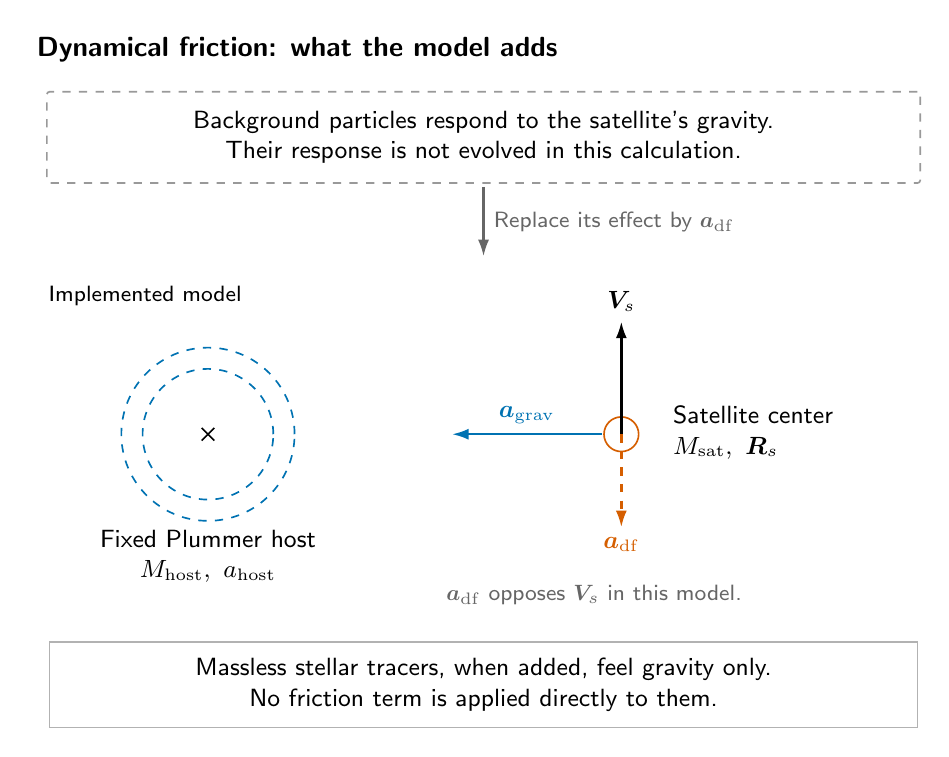
\begin{tikzpicture}[textbook diagram]
  \node[anchor=west,font=\sffamily\bfseries] at (0,4.77) {Dynamical friction: what the model adds};
  \node[draw=black!40,dashed,rounded corners=1pt,text width=106mm,align=center,inner sep=7pt] at (5.8,3.65) {Background particles respond to the satellite's gravity.\\Their response is not evolved in this calculation.};
  \draw[vector,figgray] (5.8,3.02) -- node[right,small label] {Replace its effect by $\boldsymbol a_{\rm df}$} (5.8,2.14);
  \node[small label,anchor=west] at (.15,1.64) {Implemented model};
  \coordinate (H) at (2.3,-.12); \coordinate (S) at (7.55,-.12);
  \draw[figblue,dashed] (H) circle (.83);\draw[figblue,dashed] (H) circle (1.10);
  \draw (2.22,-.20) -- (2.38,-.04);\draw (2.22,-.04) -- (2.38,-.20);
  \node[align=center] at (2.3,-1.67) {Fixed Plummer host\\$M_{\rm host},\ a_{\rm host}$};
  \draw[figred] (S) circle (.22);
  \draw[vector,figblue] ($(S)+(-.25,0)$) -- (5.40,-.12) node[midway,above] {$\boldsymbol a_{\rm grav}$};
  \draw[vector] (S) -- (7.55,1.31) node[above] {$\boldsymbol V_s$};
  \draw[vector,figred,dashed] (S) -- (7.55,-1.30) node[below] {$\boldsymbol a_{\rm df}$};
  \node[align=left,anchor=west] at (8.08,-.10) {Satellite center\\$M_{\rm sat},\ \boldsymbol R_s$};
  \node[small label,text=figgray,anchor=west] at (5.2,-2.16) {$\boldsymbol a_{\rm df}$ opposes $\boldsymbol V_s$ in this model.};
  \node[draw=black!30,text width=106mm,align=center,inner sep=6pt] at (5.8,-3.30) {Massless stellar tracers, when added, feel gravity only.\\No friction term is applied directly to them.};
\end{tikzpicture}

\caption{背景応答と実装する摩擦項の区別。上段の背景応答を直接計算する代わりに、下段では衛星中心へ$\avec_{\rm df}$を与えます。静止した平均背景に対して、摩擦は衛星速度と逆向きです。追加する質量ゼロの星には摩擦を直接掛けません。矢印の長さは力の実測値ではありません。}
\label{fig:concept-ch7-friction}
\end{figure}
\FloatBarrier
% END TikZ addition: ch07_friction_model

\subsection{速度0の見かけの特異点を避ける}
式\eqref{eq:ch7-drag}には$V_{\rm s}^{-3}$がありますが、低速では$B(X)$も$X^3$に比例して0へ向かいます。式\eqref{eq:ch7-maxwell}を小さい$X$で展開すると
\begin{equation}
 \frac{B(X)}{X^3}
 =\frac{4}{3\sqrt{\pi}}\left(1-\frac{3X^2}{5}+\frac{3X^4}{14}+\cdots\right)
 \label{eq:ch7-small-x}
\end{equation}
となります。したがって、低速極限では有限な係数を持つ$-\Vvec_{\rm s}$型の加速度になり、$\Vvec_{\rm s}=0$なら摩擦も0です。

コードでは$B/X^3$を返す関数を用意し、$X<10^{-3}$でこの級数を使います。それ以外では誤差関数を直接評価します。これは摩擦の発散を隠すために速度へ小さな数を足す操作ではなく、同じ式の連続な低速極限を計算するためです。級数の導出全体や特殊関数の実装は、本書の主要課題にはしません。
\inputcode{chap07/small-speed}
\inputcode{chap07/chandra-drag}

\texttt{gamma}は$\avec_{\rm df}=-\gamma\Vvec_{\rm s}$とまとめた係数で、一般には位置・速度に依存します。$\gamma$の単位は時間の逆数です。第1章の速度比例抵抗で使った一定の係数と、同じ関数形ではありません。\texttt{scale\_v}$=\sqrt2\sigma$を使い、$B/V^3=(B/X^3)/(\sqrt2\sigma)^3$として評価しています。

\section{RK4で軌道減衰を調べる}
\label{sec:ch7-df-integrate}
\subsection{運動方程式の右辺に動力学的摩擦を加える}
衛星中心の運動方程式は
\begin{align}
 \frac{d\Rvec_{\rm s}}{dt}&=\Vvec_{\rm s},\\
 \frac{d\Vvec_{\rm s}}{dt}&=-\frac{GM_{\rm host}\Rvec_{\rm s}}
 {(r_{\rm s}^2+a_{\rm host}^2)^{3/2}}+\avec_{\rm df}(\Rvec_{\rm s},\Vvec_{\rm s})
 \label{eq:ch7-df-ode}
\end{align}
です。重力と摩擦を合わせた加速度が速度にも依存します。位置を固定して単純に$\Delta t\avec$を加える、既習の陽的KDKのkickをそのまま流用しません。第1章のRK4を使い、各段階で位置と速度を一緒に予測します。
\inputcode{chap07/df-rhs}
\inputcode{chap07/rk4-step}

RK4の4段階の構造は第1章と同じです。最後の引数を背景・衛星のパラメータ辞書に変えただけです。中心だけの状態は形$(1,4)$で、各行の順は$[x,y,v_x,v_y]$です。摩擦を切る場合は、初期値とRK4の刻みを保ち、\texttt{friction=False}とします。摩擦あり・なしの差へ、別の積分器の差を混ぜません。

速度依存力を扱えるのがRK4だけ、という意味ではありません。分割法や陰的な更新を組み合わせる方法もありますが、ここでは既習の主要手法を再利用します。RK4は1ステップで4回の右辺評価を行うので、中心だけの1500ステップでは6000回です。

\subsection{摩擦なしの円軌道を基準にする}
同じ初期値から、摩擦あり・なしを$1.50\unit{Gyr}$まで計算します。摩擦なしでは、衛星中心は主銀河の静的な場の円軌道を回り、半径はほぼ20 kpcのままです。摩擦ありでは、今回の計算の最終半径は$\chsevenvalRdf\unit{kpc}$になりました。
\begin{figure}[htbp]\centering
\includegraphics[width=0.63\linewidth]{\figpath{ch07_df_orbit}}
\caption{固定Plummer主銀河中の衛星中心軌道。灰色破線は摩擦なし、青実線は摩擦ありです。主銀河中心は固定で、主銀河への反作用は計算しません。}\label{fig:ch7-df-orbit}
\end{figure}
\begin{figure}[htbp]\centering
\includegraphics[width=0.76\linewidth]{\figpath{ch07_df_radius}}
\caption{衛星中心半径の比較。$\ln\Lambda=\ln11$、初期半径20 kpc、RK4の刻み1 Myrです。この半径の減少はモデル内での軌道減衰であり、自己無撞着な銀河合体の完了判定ではありません。}\label{fig:ch7-df-radius}
\end{figure}

本節では$1.50\unit{Gyr}$で計算を終えます。$r_{\rm s}=0$に達するまで積分して、その時刻を合体時刻と呼ぶことはしません。衛星の質量損失、主銀河の変形、合体後の緩和が含まれていないからです。

\subsection{保存しない量の変化率を調べる}
衛星中心の比エネルギーと比角運動量を
\begin{equation}
 \varepsilon_{\rm s}=\frac{V_{\rm s}^2}{2}
 -\frac{GM_{\rm host}}{\sqrt{r_{\rm s}^2+a_{\rm host}^2}},
 \qquad \ell_{z,\rm s}=X_{\rm s}V_{y,\rm s}-Y_{\rm s}V_{x,\rm s}
 \label{eq:ch7-satellite-invariants}
\end{equation}
とします。主銀河のポテンシャルが時間に依存しないので、式\eqref{eq:ch7-df-ode}から
\begin{equation}
 \frac{d\varepsilon_{\rm s}}{dt}=\Vvec_{\rm s}\cdot\avec_{\rm df}
 =-\gamma V_{\rm s}^2\leq0,
 \qquad \frac{d\ell_{z,\rm s}}{dt}=-\gamma\ell_{z,\rm s}
 \label{eq:ch7-df-balance}
\end{equation}
を得ます。摩擦なしのときだけ両者は保存量です。$\ell_{z,\rm s}>0$の本例では、摩擦ありで角運動量も減少します。速度の大きさや運動エネルギー単独まで単調に減るとは限りません。中心へ近づくと、より深いポテンシャルの中を運動するためです。
\inputcode{chap07/df-diagnostics}

摩擦なしの最大相対誤差は、エネルギーで$\chsevenvalEno$、角運動量で$\chsevenvalLno$でした。摩擦ありの終時刻では$\varepsilon_{\rm s}(t)/|\varepsilon_{\rm s}(0)|=\chsevenvalEdf$、$\ell_{z,\rm s}(t)/\ell_{z,\rm s}(0)=\chsevenvalLdf$です。後者の変化を、保存系の数値誤差として扱わないことが重要です。
\begin{figure}[htbp]\centering
\includegraphics[width=0.76\linewidth]{\figpath{ch07_df_energy}}
\caption{衛星の比エネルギー。四角は初期エネルギーへ、保存された摩擦の仕事率を台形則で積分した値を足したものです。減少の符号と大きさが式\eqref{eq:ch7-df-balance}と整合するかを確かめます。}\label{fig:ch7-df-energy}
\end{figure}
\begin{figure}[htbp]\centering
\includegraphics[width=0.76\linewidth]{\figpath{ch07_df_angular}}
\caption{衛星の比角運動量。摩擦なしではほぼ一定、摩擦ありでは正の初期値から減少します。背景が受け取った角運動量を別の粒子で測定しているわけではありません。}\label{fig:ch7-df-angular}
\end{figure}

ここでエネルギーを受け取る背景の自由度は、実際には計算していません。式\eqref{eq:ch7-df-balance}は衛星に課した運動方程式の収支です。「衛星と主銀河を合わせた全エネルギーを数値的に保存できた」と解釈しないようにします。

\section{数値誤差とモデルの近似を区別する}
\label{sec:ch7-df-validation}
\subsection{摩擦ありでも刻みを細かくする}
RK4の刻みを4、2、1、0.5 Myrにして、同じ初期値から同じ1.50 Gyrまで計算します。隣接する二つの計算を粗い側の保存時刻にそろえ、衛星中心の位置差を
\begin{equation}
 \delta_{\rm s}(h)=\frac{\max_j|\Rvec_{{\rm s},h}(t_j)-\Rvec_{{\rm s},h/2}(t_j)|}{20\unit{kpc}}
 \label{eq:ch7-df-convergence}
\end{equation}
で測ります。主要な誤差が$Ch^4$なら、隣接する差の比は16へ近づくはずです。
\begin{table}[htbp]\centering\small
\caption{摩擦ありのRK4の刻み試験。「次行との差」は式\eqref{eq:ch7-df-convergence}です。最終行には比較相手がありません。$e_{\rm work}$は後処理の仕事積分を含む別の指標です。}\label{tab:ch7-df-resolution}
\begin{tabular}{rrrrrr}\toprule
$N_{\rm step}$ & $\Delta t$ [Myr] & 最終半径 [kpc] & 次行との $\delta_{\rm s}$ & 差の比 & $e_{\rm work}$ \\
\midrule
375 & 4.0 & 7.79814530 & $6.29\times 10^{-6}$ & --- & $1.91\times 10^{-4}$ \\
750 & 2.0 & 7.79819273 & $3.72\times 10^{-7}$ & 16.91863 & $4.89\times 10^{-5}$ \\
1500 & 1.0 & 7.79819554 & $2.25\times 10^{-8}$ & 16.48324 & $1.23\times 10^{-5}$ \\
3000 & 0.5 & 7.79819571 & --- & --- & $3.07\times 10^{-6}$ \\
\bottomrule\end{tabular}

\end{table}

細かい側の差の比は$\chsevenvalDfRatio$で、16へ近づいています。一方、これらの差は真の軌道との誤差を直接測ったものではありません。また、数値解が収束しても、Chandrasekhar近似自体の物理的な正確さが同じ精度で保証されるわけではありません。

\subsection{仕事の数値積分に由来する誤差を評価する}
式\eqref{eq:ch7-df-balance}を時間積分すれば
\begin{equation}
 \varepsilon_{\rm s}(t)-\varepsilon_{\rm s}(0)
 =\int_0^t \Vvec_{\rm s}\cdot\avec_{\rm df}\,dt'
 \label{eq:ch7-drag-work}
\end{equation}
です。右辺を、保存した仕事率から既習の台形則で近似します。この累積仕事を$\widehat W(t)$とし、
\begin{equation}
 e_{\rm work}=\max_j\frac{|\varepsilon_{\rm s}(t_j)-\varepsilon_{\rm s}(0)-\widehat W(t_j)|}
 {|\varepsilon_{\rm s}(0)|}
 \label{eq:ch7-work-error}
\end{equation}
を確認します。標準の1 Myrでは$\chsevenvalWorkResidual$でした。

表\ref{tab:ch7-df-resolution}では、この残差は刻みを半分にするとおよそ1/4になります。位置のRK4誤差が4次でも、後処理の合成台形則は2次の誤差を持つためです。\textbf{仕事積分の残差だけを見て、RK4が2次へ低下したとは判断しません。} 第3・4章と同じく、どの処理がどの誤差を持つかを分けます。

\subsection{摩擦係数の選び方による違いを比較する}
$\ln\Lambda$を1、2、$\ln11$へ変え、その他を固定します。これは刻みの試験ではなく、摩擦モデルの強さを変えた比較です。
\begin{table}[htbp]\centering\small
\caption{固定Coulomb対数を変更した中心軌道。初期半径、初期速度、主銀河、衛星質量、RK4の刻み1 Myrは共通です。}\label{tab:ch7-lambda}
\begin{tabular}{rr}\toprule
$\ln\Lambda$ & 1.50 Gyr後の半径 [kpc] \\
\midrule
1.000000 & 17.063407 \\
2.000000 & 12.143812 \\
2.397895 & 7.798196 \\
\bottomrule\end{tabular}

\end{table}

今回の値では、係数が大きいほど1.50 Gyr後の半径は小さくなりました。しかし、刻みをいくら細かくしても、どのCoulomb対数が物理的に最適かが自動的に決まるわけではありません。係数の処方、局所Maxwell近似、背景の固定、衛星の質量一定という仮定が残ります。

\begin{notebox}{中心部までの外挿には注意します}
Plummer球の中心側では、背景密度がほぼ一定になり、衛星の軌道半径も背景の代表的な長さに近づきます。本書の固定背景・局所Maxwell近似・固定Coulomb対数によるChandrasekhar公式は、この領域まで自己無撞着な応答を計算するモデルではありません。したがって、中心到達時刻を高精度な合体時刻として予測しません。これは計算を細かくすることだけでは解決しない、モデルの適用範囲の問題です。
\end{notebox}

\section{衛星の周りの星も動かす}
\label{sec:ch7-df-tracers}
中心の軌道減衰を確認した後、衛星の周りへ500個のテスト粒子を置けます。初期円盤は$R_{\rm d,sat}=1\unit{kpc}$、$R_{\max,\rm sat}=4\unit{kpc}$とし、衛星のPlummer場に対する円運動速度を与えます。生成法は第4章と同じです。位置と速度の両方へ、衛星中心の初期値を足します。

先頭1行を衛星中心、残りを星とした状態配列を作ります。原点の主銀河は固定しているため、可動中心として配列へ追加しません。星の加速度は
\begin{equation}
 \frac{d\vvec_i}{dt}=\avec_{\rm host}(\rvec_i)
 +\avec_{\rm sat}(\rvec_i-\Rvec_{\rm s})
 \label{eq:ch7-tracer-force}
\end{equation}
です。Chandrasekhar摩擦は、この式には直接加えません。摩擦が変えた衛星中心の運動を通じて、星が受ける時間依存の場が変わります。
\inputcode{chap07/df-with-tracers}

\texttt{df\_center\_rhs}を先頭行へ使い、残りの行に二つの重力場を加えます。RK4の各段階では、予測された衛星位置と星の位置を一緒に使います。衛星中心だけRK4、星だけKDKとして同期させる方法も考えられますが、本書では別の同期処理を追加せず、本章の全配列をRK4で進めます。

この追加実習では、中心だけの1 Myrより細かい0.25 Myrを標準にします。1.50 Gyrまで6000ステップ、10 Myrごとに151状態を保存します。同じ初期値を0.125 Myrでも計算したとき、全保存時刻・全星の最大位置差は$R_{\rm d,sat}$単位で$\chsevenvalSatMax$、二乗平均平方根は$\chsevenvalSatRms$でした。二つの数値解の差として記録し、自己無撞着な衛星崩壊の精度とは解釈しません。
\begin{figure}[htbp]\centering
\includegraphics[width=0.63\linewidth]{\figpath{ch07_satellite}}
\caption{摩擦ありの衛星と、その出身星の1.50 Gyr後の位置。青点は質量ゼロのテスト粒子です。星が広がっても、衛星の$M_{\rm sat}$や$a_{\rm sat}$は変更していません。表示範囲は両軸とも$\pm30\unit{kpc}$で、範囲外の粒子も計算には保持しています。}\label{fig:ch7-satellite}
\end{figure}

星が離れても、衛星質量が減り、それに応じて摩擦が弱まるという処理はありません。図\ref{fig:ch7-satellite}を衛星の自己無撞着な質量損失計算とは呼べません。さらに、有限距離から与えた衛星円盤は、主銀河を含む合成場の厳密な平衡でもありません。この追加実習の主な到達点は、中心の速度依存力と、それに伴う移動ポテンシャルの更新を同じRK4の枠組みで扱うことです。

\section{本章のまとめ}
\label{sec:ch7-summary}
本章では、固定したPlummer主銀河の中を回る衛星銀河にChandrasekhar動力学的摩擦を加えました。背景密度と速度分散は主銀河のPlummerモデルから与え、局所速度分布をMaxwell分布で近似し、Coulomb対数を一定値として扱いました。背景粒子や重力wakeそのものを計算したわけではありません。

摩擦加速度は速度にも依存するため、本書の標準的なKDKをそのまま使わず、第1章で学んだRK4へ戻りました。摩擦なしでは比エネルギーと比角運動量がほぼ保存され、摩擦ありでは両者が物理的に減少しました。仕事率とエネルギー変化の収支、時間刻みを変えた位置の自己収束を別々に確認しました。

Coulomb対数を変えることは摩擦モデルの変更であり、時間刻みを細かくする数値精度の変更とは異なります。また、衛星の周りへ星を置いても、星の離脱に応じて衛星質量を減らす処理や、主銀河の変形は含めていません。本章の軌道減衰を、自己無撞着な合体時刻の予測とはみなしません。

\chapterexercises
\paragraph{演習7.1　確認：摩擦の向きと低速極限}
式\eqref{eq:ch7-drag}を$\avec_{\rm df}=-\gamma\Vvec_{\rm s}$の形にし、$\gamma$の単位を求めてください。$\ln\Lambda\geq0$で$\Vvec_{\rm s}\cdot\avec_{\rm df}\leq0$となること、速度を反転すると摩擦も反転すること、速度0で有限な0を返すことを、コードでも確認してください。

\paragraph{演習7.2　確認：摩擦なしを基準にする}
同じ初期値とRK4の刻みで、摩擦あり・なしを計算してください。摩擦なしで半径、比エネルギー、比角運動量がほぼ一定になることを確認し、摩擦ありでそれらが変化する場合との意味の違いを説明してください。

\paragraph{演習7.3　応用：軌道減衰と数値誤差}
摩擦ありの仕事積分の残差と、隣接するRK4解の位置差を時間刻みで比較してください。仕事残差が約2次、位置差が約4次の振る舞いを示し得る理由を、それぞれに使っている数値算法から説明してください。

\paragraph{演習7.4　応用：Coulomb対数を変える}
$\ln\Lambda=1,2,\ln11$を比べ、1.50 Gyr後の衛星半径を表\ref{tab:ch7-lambda}から確認してください。この変更を時間刻みの収束試験と呼べない理由を述べてください。また、係数を大きくするほど常に現実の銀河をよく再現する、と結論できるでしょうか。

\paragraph{演習7.5　発展：衛星の星とモデルの限界}
第\ref{sec:ch7-df-tracers}節の500粒子計算を再実行し、0.25 Myrと0.125 Myrの結果を比較してください。星が衛星中心から離れても$M_{\rm sat}$を一定にしていることが、軌道減衰と質量損失の解釈にどのような制限を与えるか説明してください。主銀河の応答を計算していないことも含め、本章から決められない量を挙げてください。


\backmatter
\chapter{演習の解答・着眼点}
\markboth{演習の解答・着眼点}{}
\label{chap:answers}
第1章から第7章の演習について、数値的な答えと考えるべき点をまとめます。完全なPythonコードは完成版Notebookで確認してください。条件を変更した場合は、ここに示す標準値をそのまま期待値にせず、その条件で計算と確認をやり直してください。


\answerchapter{1}{Pythonで天体の運動を計算する}

\paragraph{1.1}
$v_c=\chonevalVc\unit{km\,s^{-1}}\simeq\chonevalVcInternal\unit{kpc\,Gyr^{-1}}$、$T=\chonevalPeriod\unit{Gyr}$です。
比エネルギーは$\varepsilon_0=\chonevalEnergy\unit{kpc^2\,Gyr^{-2}}$、
比角運動量は$\ell_{z,0}=\chonevalAngular\unit{kpc^2\,Gyr^{-1}}$です。

\paragraph{1.2}
最初のkickには$\avec(\rvec^n)$、最後のkickには$\avec(\rvec^{n+1})$を使います。
最後の加速度を再利用するので、初回1回と各ステップ1回の計201回です。
$\vvec^{n+1/2}$を使うと位置と速度の時刻がそろいません。
整数時刻の速度は、最後の半kickを加えた$\vvec^{n+1}$です。

\paragraph{1.3}
評価時刻はどちらも$t_n+\Delta t/2$ですが、予測状態はそれぞれ
$\yvec^n+(\Delta t/2)\kvec_1$と$\yvec^n+(\Delta t/2)\kvec_2$です。
第2段階では、位置の変化率にも式\eqref{eq:ch1-stage-two}で予測した速度を使います。

\paragraph{1.4}
leapfrogの最大位置誤差は順に$\choneexLfFifty$、$\choneexLfHundred$、$\choneexLfTwoHundred$でした。
RK4では$\choneexRkFifty$、$\choneexRkHundred$、$\choneexRkTwoHundred$でした。
細かい刻み側へ進むと、誤差比はそれぞれ4と16へ近づきます。
図がほぼ重なっても、同じ時刻の位置を比べれば差を測れます。

\paragraph{1.5}
軌道は$x$軸について鏡映され、回転方向が逆になります。
エネルギーは同じで、角運動量は符号が反転します。
この対称性は、成分と符号を正しく扱っているかを確認する方法にもなります。

\paragraph{1.6}
KDKは799ステップ、RK4は200ステップです。
位置誤差はそれぞれ$\chonecostLfPos$と$\chonecostRkPos$でした。
同じ時間刻みでの比較とは異なり、ここでは力評価回数をそろえて刻みを変えています。
力評価が少ないことだけから、同じコストでの精度まで決まるわけではありません。

\Needspace{7\baselineskip}
\paragraph{1.7}
$\gamma>0$なら$d\varepsilon/dt\le0$です。
今回の条件では$\varepsilon(T)/|\varepsilon(0)|\simeq\choneexDragEnergy$となりました。
初期値の$-1$より小さく、エネルギーが減っています。
これは抵抗がする仕事による変化で、保存系の数値誤差とは区別します。
解答の完全なコードは完成版Notebookで確認できます。


\answerchapter{2}{2体問題を計算する}

\paragraph{2.1}
初期位置は$\Rvec_1=(\chtwovalInitialXone,0)\unit{kpc}$、$\Rvec_2=(\chtwovalInitialXtwo,0)\unit{kpc}$です。相対円運動速度は$\chtwovalVc\unit{km\,s^{-1}}$なので、速度はそれぞれ$(0,\chtwovalInitialVone)$、$(0,\chtwovalInitialVtwo)\unit{km\,s^{-1}}$です。内部単位へ換算してから時間積分します。加速度の大きさの比は$1:2$、力の大きさの比は$1:1$です。

\paragraph{2.2}
$e=0.36$、$a_{\rm orb}=\chtwovalEllA\unit{kpc}$、$D_{\rm p}=\chtwovalEllRp\unit{kpc}$、$T_{\rm ell}=\chtwovalEllP\unit{Gyr}$です。初期動径速度が0で、その後に距離が減るため、初期位置は遠点です。標準計算の最小保存距離は$\chtwovalEllMin\unit{kpc}$でした。時間積分誤差と、近点時刻を有限の時間間隔で保存する誤差を区別します。

\paragraph{2.3}
理論値が$E(0)=0$なので、初期値に対する相対誤差は定義できません。丸めによって得た小さな非零値で割っても有効な比較にはなりません。$E_{\rm scale}=GM_1M_2/D_0$は、初期の粒子対のポテンシャルエネルギーの大きさです。放物線でも有限な基準になります。

\paragraph{2.4}
$q=1,0.5,0.1$での各天体の初期重心距離は、同じ順に
\[
\begin{aligned}
|\Rvec_1(0)|&=(\chtwovalRadiusSeriesOne)\unit{kpc},\\
|\Rvec_2(0)|&=(\chtwovalRadiusSeriesTwo)\unit{kpc}
\end{aligned}
\]
です。全質量を固定すれば$\mu$が同じなので、同じ相対初期条件は同じ相対軌道を与えます。$M_1$だけを固定する場合は、$\mu$も変わります。

\paragraph{2.5}
重心は式\eqref{eq:ch2-cm-motion}に従います。配布コードでは、重心の直線からのずれは$D_0$で割って約$\chtwovalBoostCm$でした。系全体の運動エネルギー$\Mtot V_{\rm cm}^2/2$を増やせば、相対軌道が束縛されていても$E$を正にできます。束縛性は$\varepsilon$で判断します。

\paragraph{2.6}
両天体の位置は初期位置へ、速度は初期速度の符号反転へ戻ります。本実装の最大ずれは、位置を$D_0$で割って約$\chtwovalReverseR$、速度を$v_{\rm c}$で割って約$\chtwovalReverseV$でした。これは更新の可逆性の確認であり、順方向の軌道が正確であることだけを検証する試験ではありません。位置の解析的な比較と刻み試験も必要です。

\paragraph{2.7}
$\varepsilon_0=(1.6^2/2-1)\mu/D_0=0.28\mu/D_0>0$、$e=1.6^2-1=1.56$です。標準の1000ステップで計算した$\Tc$後の距離は$\chtwovalHyperD\unit{kpc}$でした。双曲線は正の相対エネルギーを持ち、放物線と同じ初期距離から、より大きな速度で遠ざかります。完全な実装と数値出力は完成版Notebookで確認できます。


\answerchapter{3}{銀河の中で星を動かす}

\paragraph{3.1}
$\rho(0)=\chthreevalRhoZero\Msun\unit{kpc^{-3}}$、$M(<a)/M=2^{-3/2}\simeq0.353553$、$r_h=\chthreevalRhExact\unit{kpc}$です。$r=2a$の円運動速度は$\chthreevalVc\unit{km\,s^{-1}}$です。内部単位では$\chthreevalVcInt\unit{kpc\,Gyr^{-1}}$です。平面内に選んだのは軌道であり、重力を作るモデルは3次元の球なので、球殻の体積を使います。

\paragraph{3.2}
分点数は41、幅は$15/40=0.375\unit{kpc}$です。\texttt{integral[j + 1]}は、最初の分点から$j+1$番目の分点までの台形の面積の和です。$g$の単位$\Msun\unit{kpc^{-1}}$に区間幅を掛けると質量になります。$\rho$だけを半径で積分しても、質量の単位にはなりません。

\paragraph{3.3}
同じ$[0,5a]$で細かくすれば、解析的な$M(<5a)$へ近づきます。一方、幅を固定して範囲を広げる実験では、分点数も増やして中心の分解能を保ちます。解析的な範囲外の質量は、$5a,10a,20a$でそれぞれ約$(\chthreevalOutsideFractions)M$です。有限半径の内側の質量が$M$より少ないことは、積分範囲の定義から生じます。

\paragraph{3.4}
$15/2^{k+1}\leq10^{-8}$より、必要な半減回数は30です。最初の区間も$k=0$で中点を評価するため、中点評価は31回です。数値積分で定義した関数の根と、連続密度の真の半質量半径との違いは、この半減だけでは取り除けません。

\paragraph{3.5}
$f=M(<5a)/(2M)$と置くと、解析的には$r=a/\sqrt{f^{-2/3}-1}$です。$f<1/2$なので、球全体の半質量半径より小さくなります。数値計算では右辺にも同じ範囲内の積分値を使うか、解析値を使うかを明示してください。前者は両辺の積分誤差を含む、別の検証になります。

\paragraph{3.6}
$a=1.5,3,6\unit{kpc}$の順に、円運動速度は約$\chthreevalScaleVcSeries\unit{km\,s^{-1}}$、半質量半径は約$\chthreevalScaleRhSeries\unit{kpc}$です。各モデルで円にする場合は初期速度を調整します。同じ初期速度を固定すると、異なる重力場に同じ初期運動を与えた比較になり、一般には全部を円軌道にはできません。

\paragraph{3.7}
$v^2=v_r^2+\ell_z^2/r^2$を比エネルギーへ代入し、$v_r=0$とすると式\eqref{eq:ch3-turning-point}です。求めた内側の根は$r_p=\chthreevalPeri\unit{kpc}$でした。標準計算の最小保存半径は$\chthreevalPeriSaved\unit{kpc}$です。この差にはKDKの時間積分誤差と、保存時刻が近点時刻に一致しない効果が含まれます。ここで使うのは初期値からの解析的な保存量で、数値軌道の途中のエネルギーを毎回使って根を合わせ直す方法ではありません。

\bigskip
完全な実装と数値出力は完成版Notebookにあります。演習条件を変更した場合は、標準結果の数値をそのまま期待値にせず、その条件で確認をやり直してください。


\answerchapter{4}{テスト粒子で円盤銀河を作る}

\paragraph{4.1}
$\int_0^{R_{\max}}p_R\,dR=1$です。$F(R_d)=C(1)/C(5)=\chfourvalFractionRd$なので、期待粒子数は約275個です。実際の乱数標本ではこの値の周りにばらつきます。落としやすい因子は円環の面積の$R$です。

\paragraph{4.2}
区間$[1,3]$の中点なので$y=2.5$です。逆補間では$x=2$に戻ります。本章の自作関数へ$y=4$を渡すと範囲外として停止します。\texttt{np.interp}の既定値では最終点の$x=3$を返すので、それを方程式の解とみなしてはいけません。

\paragraph{4.3}
今回の初期円盤は有限範囲で規格化すると定義しています。Plummer球の全質量の定義を変更したわけではありません。標準表の逆補間は$\chfourvalHalfInterp\unit{kpc}$、解析CDFの二分法による比較値は$\chfourvalHalfExact\unit{kpc}$です。標本半径の中央値は今回$\chfourvalHalfSample\unit{kpc}$でした。最初の二つの差は表の積分・補間に由来し、標本の中央値は有限粒子数のばらつきも含みます。これはPlummer球の半質量半径約$\chfourvalPlummerHalf$ kpcとは別の量です。

\paragraph{4.4}
表\ref{tab:ch4-sampling}の値を再計算できます。ただし、異なる乱数生成環境では初期標本の照合も行います。粒子間重力を計算しないので、$N$は分布の標本数です。積分の次数は更新式と時間刻みによって決まり、$N$を増やしてもKDKは2次のままです。

\paragraph{4.5}
終点は同じ更新を通るので同じになります。標準の3000ステップでは、保存時刻数は$\chfourvalSavedSeries$個、履歴容量は$\chfourvalMemorySeries$ MBです。初期状態と最終状態も含みます。保存しない時刻の誤差の極値を見逃し得るので、出力を間引いた最大値の評価範囲を明示します。

\paragraph{4.6}
速度の2乗は変わらないので初期エネルギーは同じです。$\rvec\times\vvec$の符号は反転します。どちらも円軌道なので、連続的な数面密度は定常です。乱数で置いた任意の点の集まりについて、同時刻の粒子配置全体が$x$軸の鏡映になるとは限りません。

\paragraph{4.7}
接線速度が不足するので、粒子は初期半径から内側へ動き始めます。その後の半径は一般に振動します。今回の0.6 Gyr後の半径の中央値は$\chfourvalSubMedian\unit{kpc}$、保存時刻での最大相対エネルギー誤差は$\chfourvalSubEnergy$でした。これは非円軌道の集合であり、自己重力はありません。円軌道の解析位置は比較対象ではないので、保存量と刻みを変えた数値解どうしを使って精度を確認します。

完全な実装と実行結果は完成版Notebookに含めています。条件を変更した場合は、ここに示した標準値がそのまま期待値になるとは限りません。何を固定し、何を変更したかを記録してください。


\answerchapter{5}{2つの銀河を接近させる}

\paragraph{5.1}
中心は式\eqref{eq:ch5-center-acceleration}、星は出身にかかわらず式\eqref{eq:ch5-tracer-ode}です。$M_1\boldsymbol A_1$と$M_2\boldsymbol A_2$は同じ分母と質量積を持ち、逆符号になります。星は近くへ来た相手からも重力を受けるので、出身番号によって重力源を一つに制限しません。

\paragraph{5.2}
相対速度は式\eqref{eq:ch5-initial-values}、角運動量は$h=D_0U_t$です。$h$の単位も内部単位へそろえます。$U_p=h/D_p$を式\eqref{eq:ch5-orbital-invariants}へ代入すれば、近点でも$\varepsilon=0$です。$b\to0$では$h^2=2\mu D_p$、$U_r^2=2\mu/D_0-U_t^2$となり、点質量の式へ戻ります。

\paragraph{5.3}
正しい変換では元の$\boldsymbol s_i,\boldsymbol w_i$へ戻ります。中心速度を足し忘れると、中心に対する速度は$\boldsymbol w_i-\Vvec_k$です。すべての星に意図しない一様な速度差が入り、孤立した円軌道の初期条件ではなくなります。

\paragraph{5.4}
粒子割合は閾値の片側に何個あるかだけを数えるため、位置が変わっても粒子が閾値を越えなければ同じ値です。細かい側の最大位置差の比は今回\chfivevalLastRatio でした。終時刻、近点、質量・スケール長などを変えたときには、中心の保存量だけでなく、星の位置と調べたい指標の刻み依存性を再確認します。

\paragraph{5.5}
同じ更新を行うので、全粒子の終点と毎ステップの中心履歴は同じです。全履歴の保存時刻数は$\chfivevalSavedSeries$個になります。履歴の容量は$8\times4\times2002\times N_{\rm save}$ byteなので、それぞれ約$\chfivevalMemorySeries$ MBです。粗い出力では、保存していない時刻に起きた星の変化の極値を見逃す可能性があります。

\paragraph{5.6}
相対運動は同じで、慣性系全体の等速運動を加えただけです。今回の粒子相対位置の最大差は$R_d$単位で$\chfivevalBoostDiff$でした。一方、速度の2乗には並進速度との交差項が入るので、慣性系で測った個々のエネルギーの数値が同じである必要はありません。

\paragraph{5.7}
星の初期速度を$\vvec_i'=\Vvec_2-(\vvec_i-\Vvec_2)=2\Vvec_2-\vvec_i$とします。中心の運動は変更しません。今回の$f_1,f_2$は$\chfivevalRetroOne,\chfivevalRetroTwo$でした。出身銀河1の粒子は同じ二つの場を同じ初期条件で受け、銀河2の星から力を受けないので、軌道も変わりません。この違いは、固定形状のポテンシャルと質量ゼロの円盤という近似の中で得た応答です。自己重力、質量損失、ガスなどの効果を含む一般の合体結果まで保証しません。

\medskip
完全な実装と数値出力は完成版Notebookに含めています。数値条件を変えた場合は、この章に示した値をそのまま期待値にしないでください。


\answerchapter{6}{銀河相互作用を調べる}

\paragraph{6.1}
回転方向では円盤2の内部速度だけを反転します。近点距離では中心初期速度、質量比では中心の重心配分・相対速度と円盤2の円運動速度も変わります。本章の質量比系列は$M_1$固定なので$M_1+M_2$が変わり、第2章の全質量固定の比較とは違います。

\paragraph{6.2}
$\vvec_i=\Vvec_2+\boldsymbol w_i$から、$\boldsymbol w_i$だけを反転すると式\eqref{eq:ch6-reverse-spin}です。本実装では中心と円盤1の履歴が一致します。これは星からの反作用と星同士の重力を省いているためで、自己重力系への一般化はできません。

\paragraph{6.3}
$q=0.1$では$t_{\rm p}=\chsixvalQsmallTime\unit{Gyr}$なので、$t=0.47\unit{Gyr}$は$\tau=\chsixvalSmallTauFixed\unit{Gyr}$です。基準PPの同じ時刻は$\tau=\chsixvalBaseTau\unit{Gyr}$で、約$\chsixvalEpochDifferenceMyr$ Myr違います。本章では目標経過時間に最も近い保存時刻を選び、選択のずれも記録します。

\paragraph{6.4}
20、30、40 kpcの閾値ではPP--PRの差は$\chsixvalThresholdDifferences$でした。seed 42、43、44では、30 kpcの差は$\chsixvalSeedDifferences$です。前者は測定方法、後者は有限標本を変えています。三組で傾向が残ることは確認できますが、観測銀河全体に対する統計的な保証ではありません。

\paragraph{6.5}
標準出力では、近点5 kpcの最大差は$R_{\rm d}$単位で約$\chsixvalPfiveMax$、二乗平均平方根は約$\chsixvalPfiveRms$です。$\Delta f_k$は両方0でした。粒子が閾値の同じ側にいれば割合は変わりません。追加計算でも初期配列を再利用し、保存時刻を共通にして粒子番号ごとに比較します。

\paragraph{6.6}
一意の数値解答はありません。問い、比較条件、結果、確認、解釈の対応を重視します。非単調な結果が得られた場合も、値を選別せず、測定時刻と閾値の意味に戻って説明してください。数値計算の再現性と、物理モデルの適用範囲を両方示すことが到達目標です。

\paragraph{6.7}
比は5、8、12 kpcの順に$\chsixvalSoftRatios$です。$D\gg b$なら1へ近づきます。中心に対する全加速度と、星と中心の加速度差は別の量です。また、軌道の速さや粒子の位相・測定時刻も変わるため、この比だけで$f_k$の大小は決まりません。$b$はモデル、$\Delta t$は同じモデルを解く数値精度の設定です。完成版Notebookに、軌道を変更せずこの比を計算する短い実装を収録しています。

\answerchapter{7}{動力学的摩擦で軌道減衰を調べる}

\paragraph{7.1}
$\gamma=4\pi G^2M_{\rm sat}\rho\ln\Lambda\,B(X)/V_{\rm s}^3$で、単位は$\mathrm{Gyr^{-1}}$です。$B(0)=0$で、$X\geq0$では$B(X)\geq0$なので、$\ln\Lambda\geq0$なら$\Vvec_{\rm s}\cdot\avec_{\rm df}\leq0$です。低速では式\eqref{eq:ch7-small-x}を使って$\gamma$は有限にとどまり、$\Vvec_{\rm s}=0$なら加速度も0になります。

\paragraph{7.2}
摩擦なしの最終半径は約$\chsevenvalRno\unit{kpc}$で、比エネルギーと比角運動量の最大相対誤差はそれぞれ$\chsevenvalEno$、$\chsevenvalLno$です。摩擦ありの最終半径は$\chsevenvalRdf\unit{kpc}$です。摩擦ありの保存量の変化を、摩擦なしの場合と同じ数値誤差として扱いません。

\paragraph{7.3}
標準の1 Myrでは仕事積分の残差は$\chsevenvalWorkResidual$です。後処理に合成台形則を使うため、その残差には2次の積分誤差が入ります。一方、RK4で求めた位置の隣接解差は、細かい側で比が$\chsevenvalDfRatio$となり、4次法に対応する16へ近づきます。異なる処理の誤差次数を混同しません。

\paragraph{7.4}
$\ln\Lambda=1,2,\ln11$に対する1.50 Gyr後の半径は$\chsevenvalLambdaSeries\unit{kpc}$です。Coulomb対数は摩擦モデルの係数で、時間刻みを変える数値収束とは別です。大きい係数ほど本例では減衰が強くなりますが、どの値が現実的かは背景・衛星構造と摩擦モデルの仮定に依存します。

\paragraph{7.5}
0.25 Myrと0.125 Myrの全保存時刻・全星の最大位置差は$R_{\rm d,sat}$単位で$\chsevenvalSatMax$、二乗平均平方根は$\chsevenvalSatRms$でした。星が広がっても$M_{\rm sat}$を減らさないため、質量損失によって摩擦が弱まる効果はありません。主銀河の変形やwakeも直接計算していないので、自己無撞着な合体時刻や合体残骸の構造は本章から決められません。

\begin{thebibliography}{99}
\markboth{参考図書}{}
\addcontentsline{toc}{chapter}{参考図書}

\item[]\textbf{銀河力学・天体力学}
\bibitem{ryden2025}
Barbara Ryden, \textit{Celestial and Stellar Dynamics}, Cambridge University Press, 2025.\\
2体問題、中心力、球対称ポテンシャル、潮汐などを学ぶための入門的な参考書です。本書では、学部生が物理的な意味を確認するときの主参考書として用います。

\bibitem{bt2008}
J. Binney and S. Tremaine, \textit{Galactic Dynamics}, 2nd ed., Princeton University Press, 2008.\\
銀河ポテンシャル、Plummerモデル、軌道論、恒星系の力学、動力学的摩擦などをより詳しく調べるための標準的な参考書です。

\item[]\textbf{数値計算法}
\bibitem{sugiura2009}
杉浦洋『数値計算の基礎と応用［新訂版］―数値解析学への入門―』サイエンス社、2009年。\\
浮動小数点数と丸め誤差、補間、台形則、二分法・Newton法・割線法、Euler法・Runge--Kutta法など、本書で使う数値計算法の多くを扱っています。

\bibitem{irifuji1985}
伊理正夫・藤野和建『数値計算の常識』共立出版、1985年。\\
数値計算で生じる誤差や注意点に加え、逆補間、乱数、特定の確率分布に従う乱数の生成を扱っています。第4章の逆変換サンプリングと直接関係します。

\bibitem{simten2007}
冨阪幸治・花輪知幸・牧野淳一郎 編『シリーズ現代の天文学14 シミュレーション天文学』日本評論社、2007年。\\
天文学の数値計算を扱い、leapfrog法の時間反転対称性・シンプレクティック性と、粒子系で広く使われる理由を説明しています。本書の重力計算におけるleapfrogの位置づけと対応します。

\bibitem{kouya2021}
幸谷智紀『Python数値計算プログラミング』講談社、2021年。\\
Python 3とNumPy・SciPyを用いて数値計算を実装しながら学ぶ参考書です。浮動小数点数、補間、数値積分、Euler法・古典的Runge--Kutta法などを扱っており、本書の計算法をPythonでさらに確認したい場合の補助参考書とします。

\item[]\textbf{補足文献・公式ドキュメント}
\bibitem{pyvenv}
Python Software Foundation, \href{https://docs.python.org/3/library/venv.html}{\texttt{venv}: Creation of virtual environments}.\\
第0章のPython環境構築を補う公式文書です。

\bibitem{jupyter}
Project Jupyter, \href{https://jupyter.org/install}{Installing Jupyter}; JupyterLab Documentation.\\
第0章のNotebookとカーネル操作を補う公式文書です。

\bibitem{numpy}
NumPy Documentation, \href{https://numpy.org/doc/stable/user/absolute_beginners.html}{NumPy: the absolute basics for beginners}; \href{https://numpy.org/doc/stable/reference/generated/numpy.interp.html}{\texttt{numpy.interp}}.\\
第4章で使う線形補間の実装仕様を確認するために参照します。



\bibitem{scipy_pchip}
SciPy Documentation, \href{https://docs.scipy.org/doc/scipy/reference/generated/scipy.interpolate.PchipInterpolator.html}{\texttt{PchipInterpolator}}.\\
第4章の「もう少し詳しく」で、単調性を保つ区分的三次補間の例を紹介するときにのみ参照します。SciPyは本書の標準計算には必要ありません。

\end{thebibliography}

\noindent\small
公式ドキュメントのURLは2026年9月28日に確認しました。本書では、数値計算法について和書で扱える範囲を優先して参考図書に挙げています。より高度な常微分方程式や幾何学的積分法へ進む場合は、必要に応じて専門書を追加してください。


\end{document}
